\documentclass[hidelinks,11pt]{book}

\usepackage[T1]{fontenc}
\usepackage{microtype}
\usepackage[charter]{mathdesign}
\usepackage[margin=1in]{geometry}
\setlength{\columnsep}{.5in}
\usepackage{fancyhdr}
\usepackage[compact]{titlesec}
\usepackage{xcolor}
\usepackage{mdframed}
\usepackage{setspace}
\usepackage{mfirstuc}
\usepackage{comment}
\usepackage{graphicx,changepage}
\usepackage{pgffor}

% Make hyperrefs work
\usepackage{hyperref}

% Set up bibliography
\usepackage[semicolon,square,sort&compress,sectionbib,numbers]{natbib}
\usepackage{chapterbib}   

% Set up glossaries
\usepackage{glossaries}
%%%%%%%%%%%%%%%%%%%%%%%% Intro C %%%%%%%%%%%%%%%%%%%%%%%%%%

\newglossaryentry{portable}
{
    name=Portable,
    description={Works on multiple operating systems or machines}
}

\newglossaryentry{POSIX}
{
    name=POSIX,
    description={Portable Operating System Interface, a set of standard defined by IEEE for an operating system}
}

\newglossaryentry{linux kernel}
{
	name=Linux Kernel,
	description={A widely used operating system kernel}
}

\newglossaryentry{C}
{
	name=C,
	description={A multipurpose programming language}
}

%%%%%%%%%%%%%%%%%%%%%%%% Deadlock %%%%%%%%%%%%%%%%%%%%%%%%%%

\newglossaryentry{livelock}
{
	name=Livelock,
	description={TODO}
}

\newglossaryentry{Deadlock}{
	name=Deadlock,
	description={When a system cannot progress}
}

\newglossaryentry{RAG}{
	name=RAG,
	description={A tool for helping identify deadlock if a cycle is apprent}
}

\newglossaryentry{Coffman Conditions}{
	name=Coffman Conditions,
	description={Four necissary and sufficient conditions for deadlock}
}

\newglossaryentry{Mutual Exclusion}{
	name=Mutual Exclusion,
	description={When two processes cannot have the same resource at the same time}
}

\newglossaryentry{Circular Wait}{
	name=Circular Wait,
	description={When a set of processes are waiting for resources held by other processes}
}

\newglossaryentry{Hold and Wait}{
	name=Hold and Wait,
	description={Once a process obtains a resource, the process cannot give that resource up}
}

\newglossaryentry{pre-emption}{
	name=Pre-emption,
	description={When a process is forced to give up its resource by another process}
}

\newglossaryentry{ostrich algorithm}{
	name=Ostrich Algorithm,
	description={For a system not to care about deadlock, instead stick its head in the sand}
}


%%%%%%%%%%%%%%%%%%%%%%%% Networking %%%%%%%%%%%%%%%%%%%%%%%%%%

\newglossaryentry{octet}{
	name=Octet,
	description={Defined as exactly 8 bits. This definition is used for concreteness in IPv4}
}

\newglossaryentry{IPv4}{
	name=Internet Protocol Version 4,
	description={4th Version of the internet protocol that deals with how to route, chunk, and reassemble packets over the web}
}


\newglossaryentry{IPv6}{
	name=Internet Protocol Version 6,
	description={6th Version of the internet protocol that deals with how to route, chunk, and reassemble packets over the web}
}

\newglossaryentry{IPv4 address}{
	name=IPv4 Address,
	description={A thirty two bit number that addresses a computer}
}

\newglossaryentry{hostnames}{
  name=Hostname,
  description={Giving the machine a user-readable address that maps to an IP Address}
}

\newglossaryentry{DNS}{
  name=Domain Name Service,
  description={Service provided by ISPs among other}
}

\newglossaryentry{TCP}{
  name=Transport Control Protocol,
  description={A layer 4 protocol that deals with the reliable delivery of bytes between two computers.}
}

\newglossaryentry{Ports}{
name=Port,
description={A construct defined by layer 4 protocols that allows separate applications to share a single conenction. Each layer 4 protocol communicates with a port and application can send and receive on specific ports}
}

\newglossaryentry{Internet Engineering Task Force}{
name=Internet Engineering Task Force,
description={A group of computing professionals who oversee the development of new standards and protocols devices that communicate which each other should abide by.}
}

\newglossaryentry{packets}{
name=Packet,
description={A packet is a logical piece of data that gets sent over the internet. Packets differ from datagrams because datagrams may have multiple fragments when floating through the internet -- meaning they do not make ``sense'' without the other datagram fragments whereas one packet means something to higher level protocols}
}

\newglossaryentry{datagram}{
name=Datagram,
description={A datagram is a set of bytes that is transmitted along a path to a destination. This differs from a packet because a single datagram may not make sense to higher level protocols because it could be a fragment of a larger packet}
}

\newglossaryentry{HTTP}{
name=Hyper Text Transfer Protocol,
description={A protocol that describes how to send a VERB (GET, PUT, DELETE...) to a particular endpoint and what response to accept back. This is most commonly used to surf the web. There are a few versions of the protocol, namely 1.0, 1.1, and 2.0. 1.0 Uses one TCP connection a request, 1.1 can let you send multiple TCP connections with requests, and 2.0 is a binary wire protocol versus a plain text protocol to name a few differences}
}

\newglossaryentry{FTP}{
name=File Transfer Protocol,
description={A protocol that deals with listing and transfering files of arbitrary size to a receiver.}
}

\newglossaryentry{Ethernet}{
name=Ethernet,
description={A set of protocols that allow two computers to communicate directly over a physical Ethernet Compliant cable}
}

\newglossaryentry{WiFi}{
name=WiFi,
description={Usually referring to 802.11, wifi is a series of protocols that delimit how a computer is able to communicate wirelessly with another computer. There are many different flavors of WIFI that all provide some benefit. Most of the time, you use WIFI to communicate with your router}
}


\makeglossaries

% Set up source code highlighting
\usepackage{listings}
\usepackage[usenames,dvipsnames]{color}
\lstset{
basicstyle=\ttfamily,
columns=flexible,
breaklines=true
}

\usepackage{color}
\definecolor{greencomments}{rgb}{0,0.5,0}
\definecolor{redstrings}{rgb}{0.9,0,0}
\definecolor{mygreen}{rgb}{0,0.6,0}
\definecolor{mygray}{rgb}{0.5,0.5,0.5}
\definecolor{mymauve}{rgb}{0.58,0,0.82}
\usepackage{xcolor}

\definecolor{foreground}{HTML}{4D4D4C}
\definecolor{background}{HTML}{FFFFFF}
\definecolor{selection}{HTML}{D6D6D6}
\definecolor{line}{HTML}{EFEFEF}
\definecolor{comment}{HTML}{8E908C}
\definecolor{red}{HTML}{C82829}
\definecolor{orange}{HTML}{F5871F}
\definecolor{yellow}{HTML}{EAB700}
\definecolor{green}{HTML}{718C00}
\definecolor{aqua}{HTML}{3E999F}
\definecolor{blue}{HTML}{4271AE}
\definecolor{purple}{HTML}{8959A8}
\definecolor{window}{HTML}{EFEFEF}
% Has to be name shadecolor
\definecolor{shadecolor}{HTML}{EEEEEE}
\usepackage{framed}
\newcommand{\CodeSymbol}[1]{\textcolor{red}{#1}\bfseries}

\lstset{aboveskip=20pt,
belowskip=20pt,
xleftmargin=2cm,
xrightmargin=2cm,
xtopmargin=1cm,
xbottommargin=1cm,
framexrightmargin=1em,
framexleftmargin=1em,
frame=bt,
framextopmargin=5pt,
framexbottommargin=5pt,
backgroundcolor=\color{shadecolor},
rulecolor=\color{shadecolor},}

% Define syntax highlighting style
\usepackage{listings}
\lstdefinestyle{cstyle}
{   
	language=C,
	showspaces=false,
	showtabs=false,
	breaklines=true,
	showstringspaces=false,
	breakatwhitespace=true,
	tabsize=4,
	commentstyle=\color{comment}\itshape,
	stringstyle=\color{red}\bfseries,
	basicstyle=\ttfamily,
	keywordstyle=\color{purple}\bfseries,
	otherkeywords = {;,<<,>>,++,<,>,\#include,\#define},
	morekeywords = [2]{;,\#include,\#define},
	keywordstyle = [2]{\color{blue}\bfseries},
	morekeywords = [3]{<<, >>},
	keywordstyle = [3]{\color{yellow}},
	morekeywords = [4]{++},
	keywordstyle = [4]{\color{teal}},
	morekeywords = [5]{<,>},
	keywordstyle = [5]{\color{yellow}},
	literate={\{}{{\CodeSymbol{ \{}}}1
	{\}}{{\CodeSymbol{\}}}}1
}
\lstset{language=C,style=cstyle}

% set up quotes
\usepackage{epigraph}


% Define titles
\singlespacing
\titleformat{\section}{\vspace{1em}\large\bfseries}{\thesection. }{0em}{}
\title{\vspace{-15mm}\fontsize{24pt}{10pt}\selectfont\textbf{CS241 System Programming Wikibook}}
\date{}

% define custom environments, so we can change global style at will
\newcommand{\keyword}[1]{\texttt{#1}}
\newcommand{\todo}[1]{}
\renewcommand{\todo}[1]{{\color{red} TODO: {#1}}}
\lstnewenvironment{code}[1][]%
  {\noindent\minipage{\linewidth}\medskip 
   \lstset{basicstyle=\ttfamily\footnotesize,frame=single,#1}}
  {\endminipage}

\newenvironment{code}{\begin{lstlisting}}{\end{lstlisting}}

% For pictures
\newenvironment{proof}{\begin{shaded*}\paragraph{Proof:}}{\hfill$\square$\end{shaded*}}
\newenvironment{aside}{\begin{shaded*}\textbf{Aside}\hfill}{\end{shaded*}}
\usepackage{wrapfig}

% For table of contents and come pages
\usepackage{multicol}

\begin{document}

\raggedbottom

\pagestyle{fancy}
\fancyhf{}
\setcounter{secnumdepth}{1}
\setcounter{tocdepth}{1}

\maketitle

\begin{multicols}{2}
\tableofcontents
\end{multicols}

./introduction

\chapter{C Programming Language}

\epigraph{If you want to teach systems, don't drum up the programmers, sort the issues, and make PRs. Instead, teach them to yearn for the vast and endless C.}{Antoine de Saint-Exup\'{e}ry (Kinda)}

C is the de-facto programming language to do serious system serious programming. Why? Most kernels are written in largely in C. The Linux kernel \cite{Love} and the XNU kernel \citet{xnukernel} of which Mac OS X is based off. The Windows Kernel uses C++, but doing system programming on that is much harder on windows that UNIX for beginner system programmers. Most of you have some experience with C++, but C is a different beast entirely. You don't have nice abstractions like classes and RAII to clean up memory. You are going to have to do that yourself. C gives you much more of an opportunity to shoot yourself in the foot but lets you do thinks at a much finer grain level.

\section{History of C}

C was developed by Dennis Ritchie and Ken Thompson at Bell Labs back in 1973 \cite{Ritchie:1993:DCL:155360.155580}. Back then, we had gems of programming languages like Fortran, ALGOL, and LISP. The goal of C was two fold. One, to target the most popular computers at the time liek the PDP-7. Two, try and remove some of the lower level constructs like managing registers, programming assembly for jumps and instead create a language that had the power to express programs procedurally (as opposed to mathematically like lisp) with more readable code all while still having the ability to interface with the operating system. It sounded like a tough feat. At first, it was only used internally at Bell Labs along with the UNIX operating system. 

The first "real" standardization is with Brian Kerninghan and Dennis Ritchies book \cite{kernighan1988c}. It is still widely regarded today as the only \gls{portable} set of C instructions. The K\&R book is known as the de-facto standard for learning C.  There were different standards of C from ANSI to ISO after the Unix guides. The one that we will be mainly focusing on is the \gls{POSIX} C library. Now to get the elephant out of the room, the Linux kernel is not entirely POSIX compliant. Mostly, it is because they didn't want to pay the fee for compliance

\todo

\section{Features}

\begin{itemize}
\item Fast. There is nothing separating you and the system.
\item Simple. C and its standard library pose a simple set of portable functions.
\item Memory Management. C let's you manage your memory. This can also bite you if you have memory errors.
\item It's Everywhere. Pretty much every computer that is not embedded has some way of interfacing with C. The standard library is also everywhere. C has stood the test of time as a popular language, and it doesn't look like it is going anywhere.
\end{itemize}

\section{Crash course intro to C}

The only way to start learning C is by starting with hello world. As per the original example that Kernighan and Ritchie proposed way back when, the hello world hasn't changed that much.

\begin{code}[language=C]
#include <stdio.h>
int main(void) { 
    printf("Hello World\n");
    return 0; 
}
\end{code}

\begin{enumerate}
  \item The \keyword{\#include} directive takes the file \keyword{stdio.h} (which stands for \textbf{st}an\textbf{d}ard \textbf{i}nput and \textbf{o}utput) located somewhere in your operating system, copies the text, and substitutes it where the \keyword{\#include} was.
  \item The \keyword{int main(void)} is a function declaration. The first word \keyword{int} tells the compiler what the return type of the function is. The part before the parens (\keyword{main}) is the function name. In C, no two functions can have the same name in a single compiled program, shared libraries are a different touchy subject. Then, what comes after is the paramater list. When we give the parameter list for regular functions \keyword{(void)} that means that the compiler should error if the function is called with any arguments. For regular functions having a declaration like \keyword{void func()} means that you are allowed to call the function like \keyword{func(1, 2, 3)} because there is no delimiter \cite{CITATION_NEEDED}. In the case of \keyword{main}, it is a special function. There are many ways of declaring \keyword{main} but the ones that you will be familiar with are \keyword{int main(void)}, \keyword{int main()}, and \keyword{int main(int argc, char *argv[])}.
  \item \keyword{printf("Hello World\n");} is what we call a function call. \keyword{printf} is defined as a part of \keyword{stdio.h}. The function has been compiled and lives somewhere else on our machine. All we need to do is include the header and call the function with the appropriate parameters (a string literal \keyword{"Hello World\n"}). If you don't have the newline, the buffer will not be flushed. It is by convention that buffered IO is not flushed until a newline. \cite{CITATION_NEEDED}
  \item \keyword{return 0;}. \keyword{main} has to return an integer. By convention, \keyword{return 0} means success and anything else means failure \cite{CITATION_NEEDED}.
\end{enumerate}

\begin{code}
$ gcc main.c -o main
$ ./main
Hello World
$
\end{code}

\begin{enumerate}
\item \keyword{gcc} is short for the GNU-Compiler-Collection which has a host of compilers ready for use. The compiler infers from the extension that you are trying to compile a .c file
\item \keyword{./main} tells your shell to execute the program in the current directory called main. The program then prints out hello world
\end{enumerate}

\section{Preprocessor}

What is the preprocessor? Preprocessing is an operation that the compiler performs \textbf{before} actually compiling the program. It is a copy and paste command. Meaning that if I do the following.

\begin{code}[language=C]
#define MAX_LENGTH 10
char buffer[MAX_LENGTH]
// After
char buffer[10]
\end{code}

But there are side effects to the preprocessor. Does the following code print out.

\begin{code}[language=C]
#define min(a,b) ((a)<(b) ? (a) : (b))
int x = 4;
if(min(x++, 100)) printf("%d is six", x);
\end{code}

Macros are simple text substitution so the above example expands to \keyword{x++\ \textless{}\ 100\ ?\ x++\ :\ 100} (parenthesis omitted for clarity). Now for this case, it will probably still print 6 but consider the edge case when \keyword{x = 99}. Also consider the edge case when operator precedence comes into play.

\begin{code}[language=C]
#define min(a,b) a<b ? a : b
int x = 99;
int r = 10 + min(99, 100); // r is 100!
\end{code}

Macros are simple text substitution so the above example expands to \keyword{10\ +\ 99\ \textless{}\ 100\ ?\ 99\ :\ 100}

\subsection{C Preprocessor logical gotcha}\label{c-preprocessor-logical-gotcha}

\begin{code}[language=C]
#define ARRAY_LENGTH(A) (sizeof((A)) / sizeof((A)[0]))
int static_array[10]; // ARRAY_LENGTH(static_array) = 10
int* dynamic_array = malloc(10); // ARRAY_LENGTH(dynamic_array) = 2 or 1
\end{code}

What is wrong with the macro? Well, it works if we have a static array like the first array because \keyword{sizeof} a static array returns the bytes that array takes up, and dividing it by the \keyword{sizeof(an\_element)} would give you the number of entries. But if we use a pointer to a piece of memory, taking the sizeof the pointer and dividing it by the size of the first entry won't always give us the size of the array.

\section{Language Facilities}

\subsection{Keywords}

C has an assortment of keywords. Here are some constructs that you should know briefly as of C99.

\begin{enumerate}
\item \keyword{break} is a keyword that is used in case statements or looping statements. When used in a case statement, the program jumps to the end of the block.
\\
\begin{code}[language=C]
switch(1) {
  case 1: /* Goes to this switch */
    puts("1");
    break; /* Jumps to the end of the block */
  case 2: /* Ignores this program */
    puts("2");
    break;
} /* Continues here */
\end{code}
\\
In the context of a loop, it breaks out of the inner-most loop. The loop can be either a \keyword{for}, \keyword{while}, or \keyword{do-while} construct
\\
\begin{code}[language=C]
while(1) {
  while(2) {
    break; /* Breaks out of while(2) */
  } /* Jumps here */
  break; /* Breaks out of while(1) */
} /* Continues here */
\end{code}
\item \keyword{const} is a language level construct that tells the compiler that this data should not be modified. If one tries to change a const variable, the program will not even compile. \keyword{const} works a little differently when put before the type, the compiler flips the first type and const. Then the compiler uses a left associativity rule. Meaning that whatever is left of the pointer is constant. This is known as const-correctedness.
\\
\begin{code}[language=C]
const int i = 0; // Same as "int const i = 0"
char *str = ...; // Mutable pointer to a mutable string
const char *const_str = ...; // Mutable pointer to a constant string
char const *const_str2 = ...; // Same as above
const char *const const_ptr_str = ...;
// Constant pointer to a constant string
\end{code}

But, it is important to know that this is a compiler imposed restriction only. There are ways of getting around this and the program will run fine with defined behavior. In systems programming, the only type of memory that you can't write to is system write-protected memory.

\begin{code}[language=C]
const int i = 0; // Same as "int const i = 0"
(*((int *)&i)) = 1; // i == 1 now
const char *ptr = "hi";
*ptr = '\0'; // Will cause a Segmentation Violation
\end{code}

\item \keyword{continue} is a control flow statement that exists only in loop constructions. Continue will skip the rest of the loop body and set the program counter back to the start of the loop before.

\begin{code}[language=C]
int i = 10;
while(i--) {
  if(1) continue; /* This gets triggered */
  *((int *)NULL) = 0;
} /* Then reaches the end of the while loop */
\end{code}

\item \keyword{do \{\} while();} is another loop constructs. These loops execute the body and then check the condition at the bottom of the loop. If the condition is zero, the loop body is not executed and the rest of the program is executed. Otherwise, the loop body is executed.

\begin{code}[language=C]
int i = 1;
do {
  printf("%d\n", i--);
} while (i > 10) /* Only executed once */
\end{code}

\item \keyword{enum}
\item \keyword{extern}
\item \keyword{float}
\item \keyword{for}
\item \keyword{goto}
\item \keyword{if else else-if} are control flow keywords. There are a few ways to use these
\item \keyword{inline}
\item \keyword{register}
\item \keyword{restrict}
\item \keyword{return} is a control flow operator that exits the current function. If the function is \keyword{void} then it simply exits the functions. Otherwise another parameter follows as the return value.

\begin{code}[language=C]

\end{code}
\item \keyword{signed} is a modifier which is rarely used, but it forces an type to be signed instead of unsigned. The reasont that this is so rarely used is because types are signed by default and need to have the \keyword{unsigned} modifier to make them unsigned but it may be useful in cases where you want the compiler to default a signed type like.

\begin{code}[language=C]
int count_bits_and_sign(signed representation) {
  //...
}
\end{code}
\item \keyword{sizeof} is an operator that is evaluated at compile time, which evaluates to the number of bytes that the expression contains. Meaning that when the compiler infers the type the following code changes.
\begin{code}[language=C]
char a = 0;
printf("%zu", sizeof(a++));
\end{code}

\begin{code}[language=C]
char a = 0;
printf("%zu", 1);
\end{code}

Which then the compiler is allowed to operate on further. A note that you must have a complete definition of the type at compile time or else you may get an odd error. Consider the following
\\
\begin{code}[language=C]
// file.c
struct person;

printf("%zu", sizeof(person));

// file2.c

struct person {
  // Declarations
}
\end{code}

This code will not compile because sizeof is not able to compile \keyword{file.c} without knowing the full declaration of the \texttt{person} struct. That is typically why we either put the full declaration in a header file or we abstract the creation and the interaction away so that users cannot access the internals of our struct.

\keyword{sizeof(ary)}: \keyword{ary} is an array. Returns the number of bytes required for the entire array (5 chars + zero byte = 6 bytes) \keyword{sizeof(ptr)}: Same as sizeof(char *). Returns the number bytes required for a pointer (e.g.~4 or 8 for a 32 bit or 64-bit machine) \keyword{sizeof} is a special operator. Really it's something the compiler substitutes in before compiling the program because the size of all types is known at compile time. When you have \keyword{sizeof(char*)} that takes the size of a pointer on your machine (8 bytes for a 64-bit machine and 4 for a 32 bit and so on). When you try \keyword{sizeof(char{[}{]})}, the compiler looks at that and substitutes the number of bytes that the \textbf{entire} array contains because the total size of the array is known at compile time.

\begin{code}[language=C]
char str1[] = "will be 11";
char* str2 = "will be 8";
sizeof(str1) //11 because it is an array
sizeof(str2) //8 because it is a pointer
\end{code}

Be careful, using sizeof for the length of a string!
\item \keyword{static}
\item \keyword{struct}
\item \keyword{switch case default} Switches are essentially glorified jump statements. Meaning that you take either a byte or an integer and the control flow of the program jumps to that location.
\\
\begin{code}[language=C]
switch(/* char or int */) {
  case INT1: puts("1");
  case INT2: puts("2");
  case INT3: puts("3");
}
\end{code}

If we give a value of 2 then
\\
\begin{code}[language=C]
switch(2) {
  case 1: puts("1"); /* Doesn't run this */
  case 2: puts("2"); /* Runs this */
  case 3: puts("3"); /* Also runs this */
}
\end{code}

The break statement
\item \keyword{typedef} declares an alias for a type. Often used with structs to reduce the visual clutter of having to write `struct' as part of the type.

\begin{code}[language=C]
typedef float real; 
real gravity = 10;
// Also typedef gives us an abstraction over the underlying type used. 
// In the future, we only need to change this typedef if we
// wanted our physics library to use doubles instead of floats.

typedef struct link link_t; 
//With structs, include the keyword 'struct' as part of the original types
\end{code}

In this class, we regularly typedef functions. A typedef for a function
can be this for example

\begin{code}[language=C]
typedef int (*comparator)(void*,void*);

int greater_than(void* a, void* b){
    return a > b;
}
comparator gt = greater_than;
\end{code}

This declares a function type comparator that accepts two \keyword{void*} params and returns an integer.

\item \keyword{union}
\item \keyword{unsigned}
\item \keyword{void} is a two folded keyword. When used in terms of function or parameter definition then it means that it returns no value or accepts no parameter specifically. The following declares a function that accepts no parameters and returns nothing.

\begin{code}[language=C]
void foo(void);
\end{code}


The other use of \keyword{void} is when you are defining. A \keyword{void *} pointer is just a memory address. It is specified as an incomplete type meaning that you cannot dereference it but it can be promoted to any time to any other type. Pointer arithmetic with these pointer is undefined behavior.

\begin{code}[langauge=C]
int *array = void_ptr; // No cast needed
\end{code}

\item \keyword{volatile} is a compiler keyword. This means that the compiler should not optimize its value out. Consider the following simple function.
\\
\begin{code}[language=C]
int flag = 1;
pass_flag(&flag);
while(flag) {
    // Do things unrelated to flag
}
\end{code}
\\
The compiler may, since the internals of the while loop have nothing to do with the flag, optimize it to the following even though a function may alter the data.
\\
\begin{code}[language=C]
while(1) {
    // Do things unrelated to flag
}
\end{code}
If you put the volatile keyword then it forces the compiler to keep the variable in and perform that check. This is particularly useful for cases where you are doing multi-process or multi-threading programs so that we can
\item \keyword{while } represents the traditional \keyword{while} loop. There is a condition at the top of the loop. While that condition evaluates to a non-zero value, the loop body will be run.
\end{enumerate}

\subsection{C data types}
\begin{enumerate}
\item \keyword{char} Represents exactly one byte of data. The number of bits in a byte might vary. \keyword{unsigned char} and \keyword{signed char} mean the exact same thing. This must be aligned on a boundary (meaning you cannot use bits in between two addresses). The rest of the types will assume 8 bits in a byte.
\item \keyword{short (short int)} must be at least two bytes. This is aligned on a two byte boundary, meaning that the address must be divisble by two.
\item \keyword{int} must be at least two bytes. Again aligned to a two byte boundary. \href{http://www.open-std.org/jtc1/sc22/wg14/www/docs/n1124.pdf}{Page 34}. On most machines this will be 4 bytes.
\item \keyword{long (long int)} must be at least four bytes, which are aligned to a four byte boundary. On some machines this can be 8 bytes.
\item \keyword{long long} must be at least eight bytes, aligned to an eight byte boundary.
\item \keyword{float} represents an IEEE-754 single percision floating point number tightly specified by \href{http://ieeexplore.ieee.org/document/4610935/}{IEEE}. This will be four bytes aligned to a four byte boundary on most machines.
\item \keyword{double} represents an IEEE-754 double percision floating point number specified by the same standard, which is aligned to the nearest eight byte boundary.
\end{enumerate}

\subsection{Operators}

\section{Common C Functions}

To find more information about any functions, use the man pages. Note the man pages are organized into sections. Section 2 are System calls. Section 3 are C libraries. On the web, Google \keyword{man 7 open}. In the shell, \keyword{man -S2 open} or \keyword{man -S3 printf}

\subsection{Input/Output}

\keyword{printf} is the function with which most people are familiar. The first parameter is a format string that includes placeholders for the data to be printed. Common format specifiers are \keyword{\%s} treat the argument as a c string pointer, keep printing all characters until the NULL-character is reached; \keyword{\%d} print the argument as an integer; \keyword{\%p} print the argument as a memory address.

A simple example is shown below:

\begin{code}[language=C]
char *name = ... ; int score = ...;
printf("Hello %s, your result is %d\n", name, score);
printf("Debug: The string and int are stored at: %p and %p\n", name, &score );
// name already is a char pointer and points to the start of the array. 
// We need "&" to get the address of the int variable
\end{code}

By default, for performance, \keyword{printf} does not actually write
anything out (by calling write) until its buffer is full or a newline is
printed.

\subsection{How else can I print strings and single characters?}

Use \keyword{puts(\ name\ )} and \keyword{putchar(\ c\ )} where name is a
pointer to a C string and c is just a \keyword{char}

\subsection{How do I print to other file
streams?}\label{how-do-i-print-to-other-file-streams}

Use
\keyword{fprintf(\ \_file\_\ ,\ "Hello\ \%s,\ score:\ \%d",\ name,\ score);}
Where \_file\_ is either predefined `stdout' `stderr' or a FILE pointer
that was returned by \keyword{fopen} or \keyword{fdopen}

\subsection{Can I use file descriptors?}\label{can-i-use-file-descriptors}

Yes! Just use \keyword{dprintf(int\ fd,\ char*\ format\_string,\ ...);}
Just remember the stream may be buffered, so you will need to assure
that the data is written to the file descriptor.

\subsection{How do I print data into a C string?}

Use \keyword{sprintf} or better \keyword{snprintf}.

\begin{code}[language=C]
char result[200];
int len = snprintf(result, sizeof(result), "%s:%d", name, score);
\end{code}

snprintf returns the number of characters written excluding the
terminating byte. In the above example, this would be a maximum of 199.

The following code is vulnerable to buffer overflow. It assumes or
trusts that the input line will be no more than 10 characters, including
the terminating byte.

\begin{code}[language=C]
char buf[10];
gets(buf); // Remember the array name means the first byte of the array
\end{code}

\subsection{Should I Use Gets?}

\keyword{gets} is deprecated in C99 standard and has been removed from
the latest C standard (C11). Programs should use \keyword{fgets} or
\keyword{getline} instead.

Where each has the following structure respectively:

\begin{code}[language=C]
char *fgets (char *str, int num, FILE *stream); 

ssize_t getline(char **lineptr, size_t *n, FILE *stream);
\end{code}

Here's a simple, safe way to read a single line. Lines longer than 9
characters will be truncated:

\begin{code}[language=C]
char buffer[10];
char *result = fgets(buffer, sizeof(buffer), stdin);
\end{code}

The result is NULL if there was an error or the end of the file is
reached. Note, unlike \keyword{gets}, \keyword{fgets} copies the newline
into the buffer, which you may want to discard-

\begin{code}[language=C]
if (!result) { return; /* no data - don't read the buffer contents */}

int i = strlen(buffer) - 1;
if (buffer[i] == '\n') 
    buffer[i] = '\0';
\end{code}

One of the advantages of \keyword{getline} is that will automatically
(re-) allocate a buffer on the heap of sufficient size.

\begin{code}[language=C]
// ssize_t getline(char **lineptr, size_t *n, FILE *stream);

 /* set buffer and size to 0; they will be changed by getline */
char *buffer = NULL;
size_t size = 0;

ssize_t chars = getline(&buffer, &size, stdin);

// Discard newline character if it is present,
if (chars > 0 && buffer[chars-1] == '\n') 
    buffer[chars-1] = '\0';

// Read another line.
// The existing buffer will be re-used, or, if necessary,
// It will be `free`'d and a new larger buffer will `malloc`'d
chars = getline(&buffer, &size, stdin);

// Later... don't forget to free the buffer!
free(buffer);
\end{code}

\subsection{Parsing}

\subsection{string.h}

Why are \keyword{memcpy} and \keyword{memmove} both in \keyword{\textless{}string.h\textgreater{}}? Because strings are essentially raw memory with a null byte at the end of them! \keyword{void\ *memcpy(void\ *dest,\ const\ void\ *src,\ size\_t\ n)} moves \keyword{n} bytes starting at \keyword{src} to \keyword{dest}. \textbf{Be careful}, there is undefined behavior when the memory regions overlap. This is one of the classic works on my machine examples because many times valgrind won't be able to pick it up because it will look like it works on your machine. When the autograder hits, fail. Consider the safer version which is.

\keyword{void\ *memmove(void\ *dest,\ const\ void\ *src,\ size\_t\ n)}
does the same thing as above, but if the memory regions overlap then it
is guaranteed that all the bytes will get copied over correctly.

\subsection{stdlib.h}

To allocate space on the heap, use malloc. There's also realloc and calloc. Typically used with sizeof. e.g.~enough space to hold 10 integers

\begin{code}[language=C]
int *space = malloc(sizeof(int) * 10);
\end{code}

\subsection{Conventions/Errno}

\section{System Calls}

\subsection{What is a system call?}

\subsection{The interplay with library functions}

\subsubsection{Does \keyword{printf} call write or does write call \keyword{printf}?}

\keyword{printf} calls \keyword{write}. \keyword{printf} includes an
internal buffer so, to increase performance \keyword{printf} may not call
\keyword{write} everytime you call \keyword{printf}. \keyword{printf} is a
C library function. \keyword{write} is a system call and as we know
system calls are expensive. On the other hand, \keyword{printf} uses a
buffer which suits our needs better at that point

\section{C Memory Model}

\subsection{Structs}

\subsubsection{Struct packing}

Structs may require something called \href{http://www.catb.org/esr/structure-packing/}{padding} (tutorial).
\textbf{We do not expect you to pack structs in this course, just know that it
is there} This is because in the early days (and even now) when you have
to an address from memory you have to do it in 32bit or 64bit blocks.
This also meant that you could only request addresses that were
multiples of that. Meaning that

\begin{code}[language=C]
struct picture{
    int height;
    pixel** data;
    int width;
    char* enconding;
}
// You think picture looks like this. One box is four bytes
| h   data    w   encod |
|___ ___ ___ ___ ___ ___|
|___|___ ___|___|___ ___|
\end{code}

Would conceptually look like this

\begin{code}[language=C]
struct picture{
    int height;
    char slop1[4];
    pixel** data;
    int width;
    char slop2[4];
    char* enconding;
}

| h   ?   data    w   ?   encod |
|___ ___ ___ ___ ___ ___ ___ ___|
|___|___|___ ___|___|___|___ ___|
\end{code}

This is on a 64-bit system. This is not always the case because
sometimes your processor supports unaligned accesses. What does this
mean? Well there are two options you can set an attribute

\begin{code}[language=C]
struct __attribute__((packed, aligned(4))) picture{
    int height;
    pixel** data;
    int width;
    char* enconding;
}
// Will look like this
| h   data    w   encod |
|___ ___ ___ ___ ___ ___|
|___|___ ___|___|___ ___|

\end{code}

But now, every time I want to access \keyword{data} or \keyword{encoding},
I have to do two memory accesses. The other thing you can do is reorder
the struct, although this is not always possible

\begin{code}[language=C]
struct picture{
    int height;
    int width;
    pixel** data;
    char* enconding;
}
// You think picture looks like this
| h   w    data   encod |
|___ ___ ___ ___ ___ ___|
|___|___|___ ___|___ ___|

\end{code}

\subsection{C Null-Terminated Strings}

Strings in C are represented as characters in memory. The end of the string includes a NULL (0) byte \cite{CITATION_NEEDED}. So ``ABC'' requires four(4) bytes \keyword{{[}\textquotesingle{}A\textquotesingle{},\textquotesingle{}B\textquotesingle{},\textquotesingle{}C\textquotesingle{},\textquotesingle{}\textbackslash{}0\textquotesingle{}{]}}.
The only way to find out the length of a C string is to keep reading memory until you find the NULL byte. C characters are always exactly one byte each.

When you write a string literal \keyword{"ABC"} in an expression the string literal evaluates to a char pointer (\keyword{char\ *}), which points to the first byte/char of the string. This means \keyword{ptr} in the example below will hold the memory address of the first character in the string.

\subsubsection{String constants are constant}

\begin{code}[language=C]
char array[] = "Hi!"; // array contains a mutable copy 
strcpy(array, "OK");

char *ptr = "Can't change me"; // ptr points to some immutable memory
strcpy(ptr, "Will not work");
\end{code}

String literals are character arrays stored in the code segment of the program, which is immutable. Two string literals may share the same space in memory. An example follows:

\begin{code}[language=C]
char *str1 = "Brandon Chong is the best TA";
char *str2 = "Brandon Chong is the best TA";
\end{code}

The strings pointed to by \keyword{str1} and \keyword{str2} may actually reside in the same location in memory.

Char arrays, however, contain the literal value which has been copied from the code segment into either the stack or static memory. These following char arrays do not reside in the same place in memory.

\begin{code}[language=C]
char arr1[] = "Brandon Chong didn't write this";
char arr2[] = "Brandon Chong didn't write this";
\end{code}

\begin{code}[language=C]
char *ptr = "ABC"
\end{code}

Some common ways to initialize a string include:

\begin{code}[language=C]
char *str = "ABC";
char str[] = "ABC";
char str[]={'A','B','C','\0'};
\end{code}

\begin{code}[language=C]
char ary[] = "Hello";
char *ptr = "Hello";
\end{code}

Example

The array name points to the first byte of the array. Both \keyword{ary}
and \keyword{ptr} can be printed out:

\begin{code}[language=C]
char ary[] = "Hello";
char *ptr = "Hello";
// Print out address and contents
printf("%p : %s\n", ary, ary);
printf("%p : %s\n", ptr, ptr);
\end{code}

The array is mutable, so we can change its contents. Be careful not to write bytes beyond the end of the array though. Fortunately, "World" is no longer than "Hello"

In this case, the char pointer \keyword{ptr} points to some read-only memory (where the statically allocated string literal is stored), so we cannot change those contents.

\begin{code}[language=C]
strcpy(ary, "World"); // OK
strcpy(ptr, "World"); // NOT OK - Segmentation fault (crashes)
\end{code}

We can, however, unlike the array, we change \keyword{ptr} to point to
another piece of memory,

\begin{code}[language=C]
ptr = "World"; // OK!
ptr = ary; // OK!
ary = (..anything..) ; // WONT COMPILE
// ary is doomed to always refer to the original array.
printf("%p : %s\n", ptr, ptr);
strcpy(ptr, "World"); // OK because now ptr is pointing to mutable memory (the array)
\end{code}

What to take away from this is that pointers * can point to any type of memory while C arrays {[}{]} can only point to memory on the stack. In a more common case, pointers will point to heap memory in which case the memory referred to by the pointer CAN be modified.

\subsection{Errors}

\subsubsection{Double Frees}

A double free error is when you accidentally attempt to free the same allocation twice.

\begin{code}[language=C]
int *p = malloc(sizeof(int));
free(p);

*p = 123; // Oops! - Dangling pointer! Writing to memory we don't own anymore

free(p); // Oops! - Double free!
\end{code}

The fix is first to write correct programs! Secondly, it's good programming hygiene to reset pointers once the memory has been freed. This ensures the pointer can't be used incorrectly without the program crashing.

Fix:

\begin{code}[language=C]
p = NULL; // Now you can't use this pointer by mistake
\end{code}

\subsubsection{Buffer Overflows}

TODO

Famous example: Heart Bleed (performed a memcpy into a buffer that was of insufficient size). Simple example: implement a strcpy and forget to add one to strlen, when determining the size of the memory required.

\subsubsection{Returning pointers to automatic variables}

\begin{code}[language=C]
int *f() {
    int result = 42;
    static int imok;
    return &imok; // OK - static variables are not on the stack
    return &result; // Not OK
}
\end{code}

Automatic variables are bound to stack memory only for the lifetime of
the function. After the function returns it is an error to continue to
use the memory. \#\# Insufficient memory allocation

\begin{code}[language=C]
struct User {
   char name[100];
};
typedef struct User user_t;

user_t *user = (user_t *) malloc(sizeof(user));
\end{code}

In the above example, we needed to allocate enough bytes for the struct.
Instead, we allocated enough bytes to hold a pointer. Once we start
using the user pointer we will corrupt memory. The correct code is shown
below.

\begin{code}[language=C]
struct User {
   char name[100];
};
typedef struct User user_t;

user_t * user = (user_t *) malloc(sizeof(user_t));
\end{code}


\section{Pointers}

\subsection{Pointer Basics}

\subsubsection{Declaring a Pointer}

A pointer refers to a memory address. The type of the pointer is useful
- it tells the compiler how many bytes need to be read/written. You can
declare a pointer as follows.

\begin{code}[language=C]
int *ptr1;
char *ptr2;
\end{code}

Due to C's grammar, an \keyword{int*} or any pointer is not actually its
own type. You have to precede each pointer variable with an asterisk. As
a common gotcha, the following

\begin{code}[language=C]
int* ptr3, ptr4;
\end{code}

Will only declare \keyword{*ptr3} as a pointer. \keyword{ptr4} will
actually be a regular int variable. To fix this declaration, keep the
\keyword{*} preceding to the pointer

\begin{code}[language=C]
int *ptr3, *ptr4;
\end{code}

Keep this in mind for structs as well. If one does not typedef them, then the pointer goes after the type.

\begin{code}[language=C]
struct person *ptr3;
\end{code}

\subsubsection{Reading/Writing with pointers}

Let's say that we declare a pointer \keyword{int\ *ptr}. For the sake of
discussion, let's say that \keyword{ptr} points to memory address
\keyword{0x1000}. If we want to write to a pointer, we can dereference
and assign \keyword{*ptr}.

\begin{code}[language=C]
*ptr = 0; // Writes some memory.
\end{code}

What C will do is take the type of the pointer which is an \keyword{int}
and writes \keyword{sizeof(int)} bytes from the start of the pointer,
meaning that bytes \keyword{0x1000}, \keyword{0x1001}, \keyword{0x1002},
\keyword{0x1003} will all be zero. The number of bytes written depends on
the pointer type. It is the same for all primitive types but structs are
a little different.

\subsection{Pointer Arithmetic}

You can add an integer to a pointer. However, the pointer type is used
to determine how much to increment the pointer. For char pointers this
is trivial because characters are always one byte:

\begin{code}[language=C]
char *ptr = "Hello"; // ptr holds the memory location of 'H'
ptr += 2; //ptr now points to the first'l'
\end{code}

If an int is 4 bytes then ptr+1 points to 4 bytes after whatever ptr is
pointing at.

\begin{code}[language=C]
char *ptr = "ABCDEFGH";
int *bna = (int *) ptr;
bna +=1; // Would cause iterate by one integer space (i.e 4 bytes on some systems)
ptr = (char *) bna;
printf("%s", ptr);
/* Notice how only 'EFGH' is printed. Why is that? Well as mentioned above, when performing 'bna+=1' we are increasing the **integer** pointer by 1, (translates to 4 bytes on most systems) which is equivalent to 4 characters (each character is only 1 byte)*/
return 0;
\end{code}

Because pointer arithmetic in C is always automatically scaled by the
size of the type that is pointed to, you can't perform pointer
arithmetic on void pointers.

You can think of pointer arithmetic in C as essentially doing the
following

If I want to do

\begin{code}[language=C]
int *ptr1 = ...;
int *offset = ptr1 + 4;
\end{code}

Think

\begin{code}[language=C]
int *ptr1 = ...;
char *temp_ptr1 = (char*) ptr1;
int *offset = (int*)(temp_ptr1 + sizeof(int)*4);
\end{code}

To get the value. \textbf{Every time you do pointer arithmetic, take a
deep breath and make sure that you are shifting over the number of bytes
you think you are shifting over.}

\subsection{What is a void pointer?}

A pointer without a type (very similar to a void variable). Void pointers are used when either a datatype you're dealing with is unknown or when you're interfacing C code with other programming languages. You can think of this as a raw pointer, or just a memory address. You cannot directly read or write to it because the void type does not have a size. For Example

\begin{code}[language=C]
void *give_me_space = malloc(10);
char *string = give_me_space;
\end{code}

This does not require a cast because C automatically promotes \keyword{void*} to its appropriate type. \textbf{Note:}

\keyword{gcc} and \keyword{clang} are not total ISO-C compliant, meaning that they will let you do arithmetic on a void pointer. They will treat it as a \keyword{char *} pointer. Do not do this because it may not work with all compilers!

\section{Shell}

What do you actually use to run your program? A shell! A shell is a programming language that is running inside your terminal. A terminal is merely a window to input commands. Now, on POSIX we usually have one shell called \keyword{sh} that is linked to a POSIX compliant shell called \keyword{dash}. Most of the time, you use a shell called \keyword{bash} that is not entirely POSIX compliant but has some nifty built in features. If you want to be even more advanced, \keyword{zsh} has some more powerful features like tab complete on programs and fuzzy patterns, but that is neither here nor there. 

\subsection{Common Utilities}

\begin{enumerate}
\item \keyword{cat}
\item \keyword{diff}
\item \keyword{grep}
\item \keyword{ls}
\item \keyword{cd}
\item \keyword{man}
\item \keyword{make}
\end{enumerate}

\subsection{Syntactic}

Shells have many useful utilities like saving output to a file using redirection \keyword{>}. This overwrites the file from the beginning. If you only meant to append to the file, you can use \keyword{>>}. Unix also allows file descriptor swapping. This means that you can take the output going to one file descriptor and make it seem like its coming out of another. The most common one is \keyword{2>&1} which means take the stderr and make it seem like it is coming out of standard out. This is important because when you use \keyword{>} and \keyword{>>} they only write the standard output of the file. There are some examples below.

\begin{code}[language=console]
$ ./program > output.txt # To overwrite
$ ./program >> output.txt # To append
$ ./program 2>&1 > output_all.txt # stderr & stdout
$ ./program 2>&1 > /dev/null # don't care about any output
\end{code}

The pipe operator has a fascinating history. The UNIX philosophy is writing small programs and chaining them together to do new and interesting things. Back in the early days, hard disk space was limited and write times were slow. Brian Kernighan wanted to maintain the philosophy while also not having to write a bunch of intermediate files that take up hard drive space. So, the UNIX pipe was born. A pipe take the \keyword{stdout} of the program on its left and feeds it to the \keyword{stdin} of the program on its write. Consider the command \keyword{tee}. It can be used as a replacement for the redirection operators because tee will both write to a file and output to standard out. It also has the added benefit that it doesn't need to be the last command in the list. Meaning, that you can write an intermediate result and continue your piping.

\begin{code}[language=console]
$ ./program | tee output.txt # Overwrite
$ ./program | tee -a output.txt # Append
$ head output.txt | wc | head -n 1 # Multi pipes
$ ((head output.txt) | wc) | head -n 1 # Same as above
$ ./program | tee intermediate.txt | wc
\end{code}

The \keyword{&&} and \keyword{||} operator 

\subsection{Tips and tricks}

\begin{comment}

\subsection{\texorpdfstring{What if I really really want \keyword{printf}
to call \keyword{write} without a
newline?}{What if I really really want printf to call write without a newline?}}\label{what-if-i-really-really-want-printf-to-call-write-without-a-newline}

Use \keyword{fflush(\ FILE*\ inp\ )}. The contents of the file will be
written. If I wanted to write ``Hello World'' with no newline, I could
write it like this.

\begin{code}[language=C]
int main(){
    fprintf(stdout, "Hello World");
    fflush(stdout);
    return 0;
}
\end{code}

\subsection{\texorpdfstring{How is \keyword{perror}
helpful?}{How is perror helpful?}}\label{how-is-perror-helpful}

Let's say that you have a function call that just failed (because you
checked the man page and it is a failing return code).
\keyword{perror(const\ char*\ message)} will print the English version of
the error to stderr

\begin{code}[language=C]
int main(){
    int ret = open("IDoNotExist.txt", O_RDONLY);
    if(ret < 0){
        perror("Opening IDoNotExist:");
    }
    //...
    return 0;
}
\end{code}

\section{Parsing Input}\label{parsing-input}

\subsection{How do I parse numbers from
strings?}\label{how-do-i-parse-numbers-from-strings}

Use
\keyword{long\ int\ strtol(const\ char\ *nptr,\ char\ **endptr,\ int\ base);}
or
\keyword{long\ long\ int\ strtoll(const\ char\ *nptr,\ char\ **endptr,\ int\ base);}.

What these functions do is take the pointer to your string
\keyword{*nptr} and a \keyword{base} (ie binary, octal, decimal,
hexadecimal etc) and an optional pointer \keyword{endptr} and returns a
parsed value.

\begin{code}[language=C]
int main(){
    const char *nptr = "1A2436";
    char* endptr;
    long int result = strtol(nptr, &endptr, 16);
    return 0;
}
\end{code}

Be careful though! Error handling is tricky because the function won't
return an error code. If you give it a string that is not a number it
will return 0. This means you cant differentiate between a valid ``0''
and an invalid string. See the man page for more details on strol
behavior with invalid and out of bounds values. A safer alternative is
use to \keyword{sscanf} (and check the return value).

\begin{code}[language=C]
int main(){
    const char *input = "0"; // or "!##@" or ""
    char* endptr;
    long int parsed = strtol(input, &endptr, 10);
    if(parsed == 0){
        // Either the input string was not a valid base-10 number or it really was zero!

    }
    return 0;
}
\end{code}

\subsection{\texorpdfstring{How do I parse input using \keyword{scanf}
into
parameters?}{How do I parse input using scanf into parameters?}}\label{how-do-i-parse-input-using-scanf-into-parameters}

Use \keyword{scanf} (or \keyword{fscanf} or \keyword{sscanf}) to get input
from the default input stream, an arbitrary file stream or a C string
respectively. It's a good idea to check the return value to see how many
items were parsed. \keyword{scanf} functions require valid pointers. It's
a common source of error to pass in an incorrect pointer value. For
example,

\begin{code}[language=C]
int *data = (int *) malloc(sizeof(int));
char *line = "v 10";
char type;
// Good practice: Check scanf parsed the line and read two values:
int ok = 2 == sscanf(line, "%c %d", &type, &data); // pointer error
\end{code}

We wanted to write the character value into c and the integer value into
the malloc'd memory. However, we passed the address of the data pointer,
not what the pointer is pointing to! So \keyword{sscanf} will change the
pointer itself. i.e.~the pointer will now point to address 10 so this
code will later fail e.g.~when free(data) is called.

\subsection{How do I stop scanf from causing a buffer
overflow?}\label{how-do-i-stop-scanf-from-causing-a-buffer-overflow}

The following code assumes the scanf won't read more than 10 characters
(including the terminating byte) into the buffer.

\begin{code}[language=C]
char buffer[10];
scanf("%s",buffer);
\end{code}

You can include an optional integer to specify how many characters
EXCLUDING the terminating byte:

\begin{code}[language=C]
char buffer[10];
scanf("%9s", buffer); // reads up to 9 charactes from input (leave room for the 10th byte to be the terminating byte)
\end{code}


\section{Memory mistakes}\label{memory-mistakes}

\subsection{Buffer overflow/ underflow}\label{buffer-overflow-underflow}

\begin{code}[language=C]
#define N (10)
int i = N, array[N];
for( ; i >= 0; i--) array[i] = i;
\end{code}

C does not check that pointers are valid. The above example writes into
\keyword{array{[}10{]}} which is outside the array bounds. This can cause
memory corruption because that memory location is probably being used
for something else. In practice, this can be harder to spot because the
overflow/underflow may occur in a library call e.g.

\begin{code}[language=C]
gets(array); // Let's hope the input is shorter than my array!
\end{code}


\paragraph{\texorpdfstring{Strings require \keyword{strlen(s)+1}
bytes}{Strings require strlen(s)+1 bytes}}\label{strings-require-strlens1-bytes}

Every string must have a null byte after the last characters. To store
the string ``Hi'' it takes 3 bytes: {[}H{]} {[}i{]} {[}\0{]}.

\begin{code}[language=C]
  char *strdup(const char *input) {  /* return a copy of 'input' */
    char *copy;
    copy = malloc(sizeof(char*));     /* nope! this allocates space for a pointer, not a string */
    copy = malloc(strlen(input));     /* Almost...but what about the null terminator? */
    copy = malloc(strlen(input) + 1); /* That's right. */
    strcpy(copy, input);   /* strcpy will provide the null terminator */
    return copy;
}
\end{code}

\subsection{Using uninitialized
variables}\label{using-uninitialized-variables}

\begin{code}[language=C]
int myfunction() {
  int x;
  int y = x + 2;
...
\end{code}

Automatic variables hold garbage (whatever bit pattern happened to be in
memory). It is an error to assume that it will always be initialized to
zero.

\subsection{Assuming Uninitialized memory will be zeroed}\label{assuming-uninitialized-memory-will-be-zeroed}

\begin{code}[language=C]
void myfunct() {
   char array[10];
   char *p = malloc(10);
\end{code}

Automatic (temporary variables) are not automatically initialized to zero. Heap allocations using malloc are not automatically initialized to zero.

\section{Logic and Program flow
mistakes}\label{logic-and-program-flow-mistakes}

\subsection{Equal vs.~equality}\label{equal-vs.equality}

\begin{code}[language=C]
int answer = 3; // Will print out the answer.
if (answer = 42) { printf("I've solved the answer! It's %d", answer);}
\end{code}

\subsection{Undeclared or incorrectly prototyped
functions}\label{undeclared-or-incorrectly-prototyped-functions}

\begin{code}[language=C]
time_t start = time();
\end{code}

The system function `time' actually takes a parameter (a pointer to some
memory that can receive the time\_t structure). The compiler did not
catch this error because the programmer did not provide a valid function
prototype by including \keyword{time.h}

\subsection{Extra Semicolons}\label{extra-semicolons}

\begin{code}[language=C]
for(int i = 0; i < 5; i++) ; printf("I'm printed once");
while(x < 10); x++ ; // X is never incremented
\end{code}

However, the following code is perfectly OK.

\begin{code}[language=C]
for(int i = 0; i < 5; i++){
    printf("%d\n", i);;;;;;;;;;;;;
}
\end{code}

It is OK to have this kind of code, because the C language uses
semicolons (;) to separate statements. If there is no statement in
between semicolons, then there is nothing to do and the compiler moves
on to the next statement

\section{Other Gotchas}\label{other-gotchas}

\subsection{\texorpdfstring{Does \keyword{sizeof} do
anything?}{Does sizeof do anything?}}\label{does-sizeof-do-anything}

\begin{code}[language=C]
int a = 0;
size_t size = sizeof(a++);
printf("size: %lu, a: %d", size, a);
\end{code}

What does the code print out?

\begin{code}[language=C]
size: 4, a: 0
\end{code}

Because sizeof is not actually evaluated at runtime. The compiler
assigns the type of all expressions and discards the extra results of
the expression.

\section{Strings, Structs, and
Gotcha's}\label{strings-structs-and-gotchas}

\section{So what's a string?}\label{so-whats-a-string}

\begin{figure}[htbp]
\centering
\includegraphics{https://i.imgur.com/CgsxyZb.png}
\caption{String}
\end{figure}

In C we have
\href{https://en.wikipedia.org/wiki/Null-terminated_string}{Null
Terminated} strings rather than
\href{https://en.wikipedia.org/wiki/String_(computer_science)\#Length-prefixed}{Length
Prefixed} for historical reasons. What that means for your average
everyday programming is that you need to remember the null character! A
string in C is defined as a bunch of bytes until you reach `\0' or the
Null Byte.

\subsection{Two places for strings}\label{two-places-for-strings}

Whenever you define a constant string (ie one in the form
\keyword{char*\ str\ =\ "constant"}) That string is stored in the
\emph{data} or \emph{code} segment that is \textbf{read-only} meaning
that any attempt to modify the string will cause a segfault.

If one, however, \keyword{malloc}'s space, one can change that string to
be whatever they want.

\subsection{Memory Mismanagement}\label{memory-mismanagement}

One common gotcha is when you write the following

\begin{code}[language=C]
char* hello_string = malloc(14);
                       ___ ___ ___ ___ ___ ___ ___ ___ ___ ___ ___ ___ ___ ___
// hello_string ----> | g | a | r | b | a | g | e | g | a | r | b | a | g | e |
                                                                              
hello_string = "Hello Bhuvan!";
// (constant string in the text segment)
// hello_string ----> [ "H" , "e" , "l" , "l" , "o" , " " , "B" , "h" , "u" , "v" , "a" , "n" , "!" , "\0" ]
                       ___ ___ ___ ___ ___ ___ ___ ___ ___ ___ ___ ___ ___ ___
// memory_leak -----> | g | a | r | b | a | g | e | g | a | r | b | a | g | e |
                                                                              
hello_string[9] = 't'; //segfault!!
\end{code}

What did we do? We allocated space for 14 bytes, reassigned the pointer
and successfully segfaulted! Remember to keep track of what your
pointers are doing. What you probably wanted to do was use a
\keyword{string.h} function \keyword{strcpy}.

\begin{code}[language=C]
strcpy(hello_string, "Hello Bhuvan!");
\end{code}

\subsection{Remember the NULL byte!}\label{remember-the-null-byte}

Forgetting to NULL terminate a string is a big affect on the strings!
Bounds checking is important. The heart bleed bug mentioned earlier in
the wiki book is partially because of this.

\subsection{Where can I find an In-Depth and Assignment-Comprehensive
explanation of all of these
functions?}\label{where-can-i-find-an-in-depth-and-assignment-comprehensive-explanation-of-all-of-these-functions}

\href{https://linux.die.net/man/3/string}{Right Here!}

\subsection{\texorpdfstring{String Information/Comparison:
\keyword{strlen}
\keyword{strcmp}}{String Information/Comparison: strlen strcmp}}\label{string-informationcomparison-strlen-strcmp}

\keyword{int\ strlen(const\ char\ *s)} returns the length of the string
not including the null byte

\keyword{int\ strcmp(const\ char\ *s1,\ const\ char\ *s2)} returns an
integer determining the lexicographic order of the strings. If s1 where
to come before s2 in a dictionary, then a -1 is returned. If the two
strings are equal, then 0. Else, 1.

With most of these functions, they expect the strings to be readable and
not NULL but there is undefined behavior when you pass them NULL.

\subsection{\texorpdfstring{String Alteration: \keyword{strcpy}
\keyword{strcat}
\keyword{strdup}}{String Alteration: strcpy strcat strdup}}\label{string-alteration-strcpy-strcat-strdup}

\keyword{char\ *strcpy(char\ *dest,\ const\ char\ *src)} Copies the
string at \keyword{src} to \keyword{dest}. \textbf{assumes dest has enough
space for src}

\keyword{char\ *strcat(char\ *dest,\ const\ char\ *src)} Concatenates the
string at \keyword{src} to the end of destination. \textbf{This function
assumes that there is enough space for \keyword{src} at the end of
destination including the NULL byte}

\keyword{char\ *strdup(const\ char\ *dest)} Returns a \keyword{malloc}'ed
copy of the string.

\subsection{\texorpdfstring{String Search: \keyword{strchr}
\keyword{strstr}}{String Search: strchr strstr}}\label{string-search-strchr-strstr}

\keyword{char\ *strchr(const\ char\ *haystack,\ int\ needle)} Returns a
pointer to the first occurrence of \keyword{needle} in the
\keyword{haystack}. If none found, \keyword{NULL} is returned.

\keyword{char\ *strstr(const\ char\ *haystack,\ const\ char\ *needle)}
Same as above but this time a string!

\subsection{\texorpdfstring{String Tokenize:
\keyword{strtok}}{String Tokenize: strtok}}\label{string-tokenize-strtok}

A dangerous but useful function strtok takes a string and tokenizes it.
Meaning that it will transform the strings into separate strings. This
function has a lot of specs so please read the man pages a contrived
example is below.

\begin{code}[language=C]
#include <stdio.h>
#include <string.h>

int main(){
    char* upped = strdup("strtok,is,tricky,!!");
    char* start = strtok(upped, ",");
    do{
        printf("%s\n", start);
    }while((start = strtok(NULL, ",")));
    return 0;
}
\end{code}

\textbf{Output}

\begin{code}[language=C]
strtok
is
tricky
!!
\end{code}

What happens when I change \keyword{upped} like this?

\begin{code}[language=C]
char* upped = strdup("strtok,is,tricky,,,!!");
\end{code}

\section{\texorpdfstring{So what's a \keyword{struct}?}{So what's a struct?}}\label{so-whats-a-struct}

In low-level terms, a struct is just a piece of contiguous memory,
nothing more. Just like an array, a struct has enough space to keep all
of its members. But unlike an array, it can store different types.
Consider the contact struct declared above

\begin{code}[language=C]
struct contact {
    char firstname[20];
    char lastname[20];
    unsigned int phone;
};

struct contact bhuvan;
\end{code}

\textbf{Brief aside}

\begin{code}[language=C]
/* a lot of times we will do the following typdef
 so we can just write contact contact1 */

typedef struct contact contact;
contact bhuvan;

/* You can also declare the struct like this to get
 it done in one statement */
typedef struct optional_name {
    ...
} contact;
\end{code}

If you compile the code without any optimizations and reordering, you
can expect the addresses of each of the variables to look like this.

\begin{code}[language=C]
&bhuvan           // 0x100
&bhuvan.firstname // 0x100 = 0x100+0x00
&bhuvan.lastname  // 0x114 = 0x100+0x14
&bhuvan.phone     // 0x128 = 0x100+0x28
\end{code}

Because all your compiler does is say `hey reserve this much space, and
I will go and calculate the offsets of whatever variables you want to
write to'. The offsets are where the variable starts at. The phone variables starts
at the \keyword{0x128}th bytes and continues for sizeof(int) bytes, but
not always. \textbf{Offsets don't determine where the variable ends
though}. Consider the following hack that you see in a lot of kernel
code.

\begin{code}[language=C]

typedef struct {
    int length;
    char c_str[0];
} string;

const char* to_convert = "bhuvan";
int length = strlen(to_convert);

// Let's convert to a c string
string* bhuvan_name;
bhuvan_name = malloc(sizeof(string) + length+1);
/*
Currently, our memory looks like this with junk in those black spaces
                ___ ___ ___ ___ ___ ___ ___ ___ ___ ___ ___
 bhuvan_name = |   |   |   |   |   |   |   |   |   |   |   |
                                                           
*/


bhuvan_name->length = length;
/*
This writes the following values to the first four bytes
The rest is still garbage
                ___ ___ ___ ___ ___ ___ ___ ___ ___ ___ ___
 bhuvan_name = | 0 | 0 | 0 | 6 |   |   |   |   |   |   |   |
                                                           
*/


strcpy(bhuvan_name->c_str, to_convert);
/*
Now our string is filled in correctly at the end of the struct

                ___ ___ ___ ___ ___ ___ ___ ___ ___ ___ ____
 bhuvan_name = | 0 | 0 | 0 | 6 | b | h | u | v | a | n | \0 |
                                                           ‾
*/

strcmp(bhuvan_name->c_str, "bhuvan") == 0 //The strings are equal!
\end{code}

\end{comment}

\section{Common Bugs}

\begin{code}[language=C]
void mystrcpy(char*dest, char* src) { 
  // void means no return value   
  while( *src ) { dest = src; src ++; dest++; }  
}
\end{code}

In the above code it simply changes the dest pointer to point to source
string. Also the nuls bytes are not copied. Here's a better version -

\begin{code}[language=C]
  while( *src ) { *dest = *src; src ++; dest++; } 
  *dest = *src;
\end{code}

Note it's also usual to see the following kind of implementation, which
does everything inside the expression test, including copying the nul
byte.

\begin{code}[language=C]
  while( (*dest++ = *src++ )) {};
\end{code}

\section{Topics}

\begin{itemize}
\tightlist
\item
  C Strings representation
\item
  C Strings as pointers
\item
  char p{[}{]}vs char* p
\item
  Simple C string functions (strcmp, strcat, strcpy)
\item
  sizeof char
\item
  sizeof x vs x*
\item
  Heap memory lifetime
\item
  Calls to heap allocation
\item
  Deferencing pointers
\item
  Address-of operator
\item
  Pointer arithmetic
\item
  String duplication
\item
  String truncation
\item
  double-free error
\item
  String literals
\item
  Print formatting.
\item
  memory out of bounds errors
\item
  static memory
\item
  fileio POSIX vs.~C library
\item
  C io fprintf and printf
\item
  POSIX file IO (read, write, open)
\item
  Buffering of stdout
\end{itemize}

\section{Questions/Exercises}

\begin{itemize}
\item
  What does the following print out?

\begin{code}[language=C]
int main(){
fprintf(stderr, "Hello ");
fprintf(stdout, "It's a small ");
fprintf(stderr, "World\n");
fprintf(stdout, "place\n");
return 0;
}
\end{code}
\item
  What are the differences between the following two declarations? What
  does \keyword{sizeof} return for one of them?

\begin{code}[language=C]
char str1[] = "bhuvan";
char *str2 = "another one";
\end{code}
\item
  What is a string in c?
\item
  Code up a simple \keyword{my\_strcmp}. How about \keyword{my\_strcat},
  \keyword{my\_strcpy}, or \keyword{my\_strdup}? Bonus: Code the functions
  while only going through the strings \emph{once}.
\item
  What should the following usually return?

\begin{code}[language=C]
int *ptr;
sizeof(ptr);
sizeof(*ptr);
\end{code}
\item
  What is \keyword{malloc}? How is it different than \keyword{calloc}.
  Once memory is \keyword{malloc}ed how can I use \keyword{realloc}?
\item
  What is the \keyword{\&} operator? How about \keyword{*}?
\item
  Pointer Arithmetic. Assume the following addresses. What are the
  following shifts?

\begin{code}[language=C]
char** ptr = malloc(10); //0x100
ptr[0] = malloc(20); //0x200
ptr[1] = malloc(20); //0x300
\end{code}

  \begin{itemize}
  \tightlist
  \item
    \keyword{ptr\ +\ 2}
  \item
    \keyword{ptr\ +\ 4}
  \item
    \keyword{ptr{[}0{]}\ +\ 4}
  \item
    \keyword{ptr{[}1{]}\ +\ 2000}
  \item
    \keyword{*((int)(ptr\ +\ 1))\ +\ 3}
  \end{itemize}
\item
  How do we prevent double free errors?
\item
  What is the printf specifier to print a string, \keyword{int}, or
  \keyword{char}?
\item
  Is the following code valid? If so, why? Where is \keyword{output}
  located?

\begin{code}[language=C]
char *foo(int var){
static char output[20];
snprintf(output, 20, "%d", var);
return output;
}
\end{code}
\item
  Write a function that accepts a string and opens that file prints out
  the file 40 bytes at a time but every other print reverses the string
  (try using POSIX API for this).
\item
  What are some differences between the POSIX filedescriptor model and
  C's \keyword{FILE*} (ie what function calls are used and which is
  buffered)? Does POSIX use C's \keyword{FILE*} internally or vice versa?
\end{itemize}

\bibliographystyle{plainnat}
\bibliography{introc/introc}

%\chapter{Processes}

\epigraph{Who needs process isolation?}{Intel Marketing on Meltdown and Spectre}

To understand what a process is, you need to understand what an operating system is.
An operating system is a program that provides an interface between hardware and user software as well as providing a set of tools that the software can use.
The operating system manages hardware and gives user programs a uniform way of interacting with hardware as long as the operating system can be installed on that hardware.
Although this idea sounds like it is the end-all, we know that there are many different operating systems with their own quirks and standards.
As a solution to that, there is another layer of abstraction: POSIX or portable operating systems interface.
This is a standard (or many standards now) that an operating system must implement to be POSIX compatible -- most systems that we'll be studying are almost POSIX compatible due more to political reasons.

Before we talk about POSIX systems, we should understand what the idea of a kernel is generally.
In an operating system (OS), there are two spaces: kernel space and user space.
Kernel space is a power operating mode that allows the system to interact with the hardware and has the potential to destroy your machine.
User space is where most applications run because they don't need this level of power for every operation.
When a user space program needs additional power, it interacts with the hardware through a system call that is conducted by the kernel.
This adds a layer of security so that normal user programs can't destroy your entire operating system.
For the purposes of our class, we'll talk about single machine multiple user operating systems.
This is where there is a central clock on a standard laptop or desktop.
Other OSes relax the central clock requirement (distributed) or the ``standardness'' of the hardware (embedded systems).
Other invariants make sure events happen at particular times too.

The operating system is made up of many different pieces.
There may be a program running to handle incoming USB connections, another one to stay connected to the network, etc.
The most important one is the kernel -- although it might be a set of processes -- which is the heart of the operating system.
The kernel has many important tasks.
The first of which is booting.

\begin{enumerate}
\item The computer hardware executes code from read-only memory, called firmware.
\item The firmware executes a bootloader, which often conforms to the Extensible Firmware Interface (\keyword{EFI}), which is an interface between the system firmware and the operating system.
\item The bootloader's boot manager loads the operating system kernels, based on the boot settings.
\item
  Your kernel executes \keyword{init} to \href{https://en.wikipedia.org/wiki/Bootstrapping}{bootstrap} itself from nothing.
\item The kernel executes startup scripts like starting networking and USB handling.
\item The kernel executes userland scripts like starting a desktop, and you get to use your computer!
\end{enumerate}

When a program is executing in user space, the kernel provides some important services to programs in User space.

\begin{itemize}
\item Scheduling processes and threads
\item Handling synchronization primitives (futexes, mutexes, semaphores, etc.)
\item Providing system calls such as \keyword{write} or \keyword{read}
\item Managing virtual memory and low-level binary devices such as \keyword{USB} drivers
\item Managing filesystems
\item Handling communication over networks
\item Handling communication between processes
\item Dynamically linking libraries
\item The list goes on and on.
\end{itemize}

The kernel creates the first process \keyword{init.d} (an alternative is system.d).
\emph{init.d} boots up programs such as graphical user interfaces, terminals, etc -- by default, this is the only process explicitly created by the system.
All other processes are instantiated by using the system calls \keyword{fork} and \keyword{exec} from that single process.

\section{File Descriptors}

Although these were mentioned in the last chapter, we are going to give a quick reminder about file descriptors.
A zine from Julia Evans gives some more details \cite{evans_2018}.

The kernel keeps track of the file descriptors and what they point to.
Later we will learn two things: that file descriptors need not point to actual files and that the operating system keeps track of them.

Notice that file descriptors may be reused between processes, but inside of a process, they are unique.
File descriptors may have a notion of position. These are known as seekable streams.
A program can read a file on disk completely because the OS keeps track of the position in the file, an attribute that belongs to your process as well.

Other file descriptors point to network sockets and various other pieces of information, that are not seekable streams.

\section{Processes}

A process is an instance of a computer program that may be running.
Processes have many resources at their disposal.
At the start of each program, a program gets one process, but each program can make more processes.
A program consists of the following:

\begin{itemize}
    \item A binary format: This tells the operating system about the various sections of bits in the binary -- which parts are executable, which parts are constants, which libraries to include etc.
    \item A set of machine instructions
    \item A number denoting which instruction to start from
    \item Constants
    \item Libraries to link and where to fill in the address of those libraries
\end{itemize}

Processes are very powerful, but they are isolated!

That means that by default, no process can communicate with another process.

This is very important because in complex systems (like the University of Illinois Engineering Workstations), it is likely that different processes will have different privileges.
One certainly doesn't want the average user to be able to bring down the entire system, by either purposely or accidentally modifying a process.
As most of you have realized by now, if you stuck the following code snippet into a program, the variables would not be shared between two parallel invocations of the program.

\begin{lstlisting}[language=C]
int secrets;
secrets++;
printf("%d\n", secrets);
\end{lstlisting}

On two different terminals, they would both print out 1 not 2.
Even if we changed the code to attempt to affect other process instances, there would be no way to change another process' state unintentionally.
However, there are other intentional ways to change the program states of other processes.

\section{Process Contents}

\subsection{Memory Layout}

When a process starts, it gets its own address space.
Each process gets the following.

\begin{itemize}
\item \textbf{A Stack}.
The stack is the place where automatically allocated variables and function call return addresses are stored.
Every time a new variable is declared, the program moves the stack pointer down to reserve space for the variable.
This segment of the stack is writable but not executable.
This behavior is controlled by the no-execute (NX) bit, sometimes called the W\^X (write XOR execute) bit, which helps prevent malicious code, such as \keyword{shellcode} from being run on the stack.

If the stack grows too far -- meaning that it either grows beyond a preset boundary or intersects the heap -- the program will stack overflow error, most likely resulting in a SEGFAULT.
\textbf{The stack is statically allocated by default; there is only a certain amount of space to which one can write.}

\item \textbf{A Heap}.
The heap is a contiguous, expanding region of memory \cite{mallocinternals}.
If a program wants to allocate an object whose lifetime is manually controlled or whose size cannot be determined at compile-time, it would want to create a heap variable.

The heap starts at the top of the text segment and grows upward, meaning \keyword{malloc} may push the heap boundary -- called the program break -- upward.

We will explore this in more depth in our chapter on memory allocation.
This area is also writable but not executable.
One can run out of heap memory if the system is constrained or if a program run out of addresses, a phenomenon that is more common on a 32-bit system.

\item \textbf{A Data Segment}

  This segment contains two parts, an initialized data segment, and an uninitialized segment.
  Furthermore, the initialized data segment is divided into a readable and writable section.

\begin{itemize}
    \item \textbf{Initialized Data Segment}
          This contains all of a program's globals and any other static variables.

          This section starts at the end of the text segment and starts at a constant size because the number of globals is known at compile time. The end of the data segment is called the \keyword{program break} and can be extended via the use of brk / sbrk.

          This section is writable \cite[P. 124]{van1994expert}.
          Most notably, this section contains variables that were initialized with a static initializer, as follows:

\begin{lstlisting}[language=C]
int global = 1;
\end{lstlisting}

    \item \textbf{Uninitialized Data Segment / BSS}
          BSS stands for an old assembler operator known as Block Started by Symbol.

          This contains all of your globals and any other static duration variables that are implicitly zeroed out.

          Example:
\begin{lstlisting}[language=C]
int assumed_to_be_zero;
\end{lstlisting}

          It is not an error to assume that this will be zero; otherwise, we would have a security risk involving isolation from other processes.

          They just get put in a different section to speed up process start up time.

          This section starts at the end of the data segment and is also static in size because the amount of globals is known at compile time.
          
          Currently, both the initialized and BSS data segments are combined and referred to as the data segment \cite[P. 124]{van1994expert}, despite being somewhat different in purpose.

    \item \textbf{A Text Segment}.
          This is where all executable instructions are stored, and is readable (function pointers) but not writable.

          The program counter moves through this segment executing instructions one after the other.

          It is important to note that this is the only executable section of the program, by default.

          If a program's code while it's running, the program most likely will SEGFAULT.

          There are ways around it, but we will not be exploring these in this course.

          Why doesn't it always start at zero?
          This is because of a security feature called \href{https://en.wikipedia.org/wiki/Address_space_layout_randomization}{address space layout randomization}.

          The reasons for and explanation about this is outside the scope of this class, but it is good to know about its existence.

          Having said that, this address can be made constant, if a program is compiled with the DEBUG flag.
\end{itemize}
\end{itemize}


\begin{figure}[H]
\centering
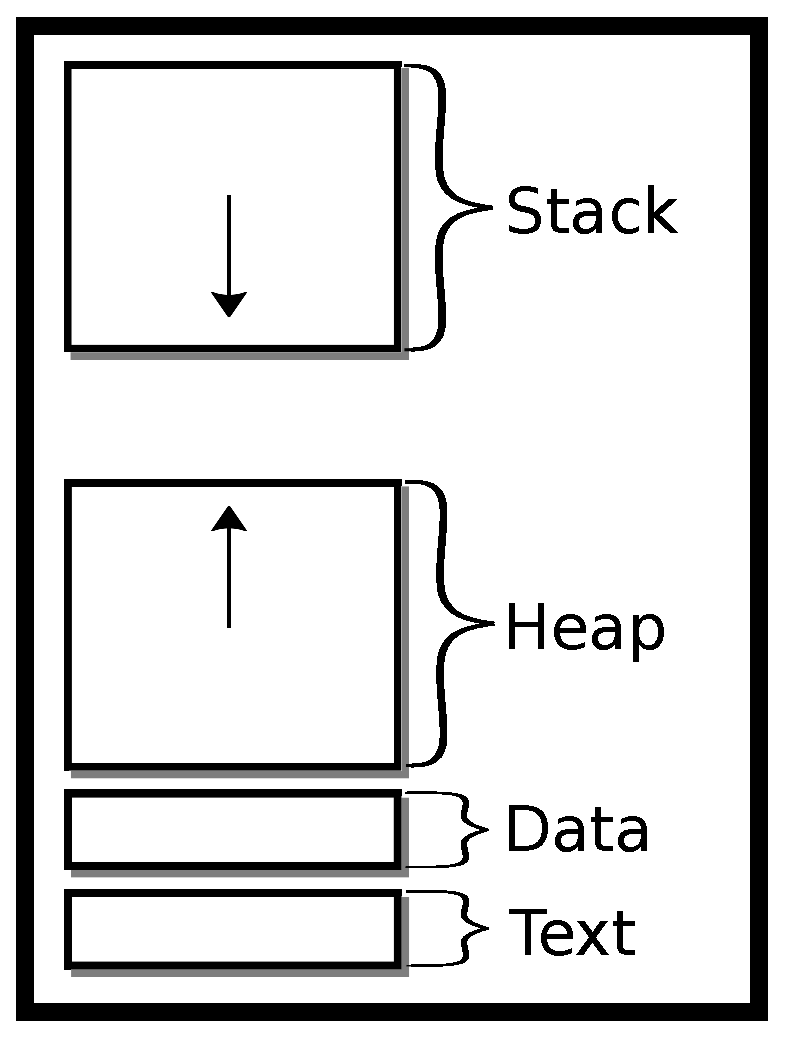
\includegraphics[width=.3\textwidth]{processes/drawings/address_space.eps}
\caption{Process address space}
\end{figure}



\subsection{Other Contents}

To keep track of all these processes, your operating system gives each process a number called the process ID (PID).
Processes are also given the PID of their parent process, called parent process ID (\keyword{PPID}).
Every process has a parent, that parent could be \keyword{init.d}.

Processes could also contain the following information:

\begin{itemize}
    \item Running State - Whether a process is getting ready, running, stopped, terminated, etc. (more on this is covered in the chapter on Scheduling).
    \item File Descriptors - A list of mappings from integers to real devices (files, USB flash drives, sockets)
    \item Permissions - What \keyword{user} the file is running on and what \keyword{group} the process belongs to.
          The process can then only perform operations based on the permissions given to the \keyword{user} or \keyword{group}, such as accessing files.
          There are tricks to make a program not be the user who started the program i.e. \keyword{sudo} takes a program that a \keyword{user} starts and executes it as \keyword{root}.
          More specifically, a process has a real user ID (identifies the owner of the process), an effective user ID (used for non-privileged users trying to access files only accessible by superusers), and a saved user ID (used when privileged users perform non-privileged actions).
    \item Arguments - a list of strings that tell your program what parameters to run under.
    \item Environment Variables - a list of key-value pair strings in the form \keyword{NAME=VALUE} that one can modify. These are often used to specify paths to libraries and binaries, program configuration settings, etc.
\end{itemize}

According to the POSIX specification, a process only needs a thread and address space, but most kernel developers and users know that only these aren't enough \cite{process_def}.

\section{Intro to Fork}

\subsection{A word of warning}

Process forking is a powerful and dangerous tool.
If you make a mistake resulting in a fork bomb, \textbf{you can bring down an entire system}.
To reduce the chances of this, limit your maximum number of processes to a small number e.g. 40 by typing \keyword{ulimit\ -u\ 40} into a command line.
Note, this limit is only for the user, which means if you fork bomb, then you won't be able to kill all of the processes you just created since calling \keyword{killall} requires your shell to \keyword{fork()} \ldots{} isn't this ironic? One solution is to spawn another shell instance as another user (for example root) beforehand and kill processes from there.

Another is to use the built-in \keyword{exec} command to kill all the user processes (you only have one attempt at this).

Finally, you could reboot the system, but you only have one shot at this with the exec function.

When testing fork() code, ensure that you have either root and/or physical access to the machine involved.
If you must work on fork() code remotely, remember that \textbf{kill -9 -1} will save you in the event of an emergency.
Fork can be \textbf{extremely} dangerous if you aren't prepared for it. \textbf{You have been warned.}

\subsection{Fork Functionality}

The \keyword{fork} system call clones the current process to create a new process, called a child process.
This occurs by duplicating the state of the existing process with a few minor differences.
\begin{itemize}
    \item The child process does not start from main. Instead, it executes the next line after the \keyword{fork()} just as the parent process does.
    \item Just as a side remark, in older UNIX systems, the entire address space of the parent process was directly copied regardless of whether the resource was modified or not. The current behavior is for the kernel to perform a \href{https://en.wikipedia.org/wiki/Copy-on-write}{copy-on-write}, which saves a lot of resources, while being very time efficient \cite[Copy-on-write section]{Bovet:2005:ULK:1077084}.
\end{itemize}

Here is a very simple example:

\begin{minted}{C}
printf("I'm printed once!\n");
fork();
// Now two processes running if fork succeeded
// and each process will print out the next line.
printf("This line twice!\n");
\end{minted}

Here is a simple example of this address space cloning.
The following program may print out 42 twice - but the \keyword{fork()} is after the \keyword{printf}!? Why?

\begin{minted}{C}
#include <unistd.h> /*fork declared here*/
#include <stdio.h> /* printf declared here*/
int main() {
  int answer = 84 >> 1;
  printf("Answer: %d", answer);
  fork();
  return 0;
}
\end{minted}

The \keyword{printf} line \emph{is} executed only once however notice that the printed contents are not flushed to standard out.
There's no newline printed, we didn't call \keyword{fflush}, or change the buffering mode.
The output text is therefore still in process memory waiting to be sent.
When \keyword{fork()} is executed the entire process memory is duplicated including the buffer.
Thus, the child process starts with a non-empty output buffer which may be flushed when the program exits.
We say may because the contents may be unwritten given a bad program exit as well.

To write code that is different for the parent and child process, check the return value of \keyword{fork()}.
If \keyword{fork()} returns -1, that implies something went wrong in the process of creating a new child.
One should check the value stored in \emph{errno} to determine what kind of error occurred.
Common errors include \keyword{EAGAIN} and \keyword{ENOENT} Which are essentially "try again -- resource temporarily unavailable", and "no such file or directory".

Similarly, a return value of 0 indicates that we are operating in the context of the child process, whereas a positive integer shows that we are in the context of the parent process.

The positive value returned by \keyword{fork()} is the process id (\emph{pid}) of the child.

A way to remember what is represented by the return value of fork is, that the child process can find its parent - the original process that was duplicated - by calling \keyword{getppid()} - so does not need any additional return information from \keyword{fork()}. However, the parent process may have many child processes, and therefore needs to be explicitly informed of its child PIDs.

According to the POSIX standard, every process only has a single parent process.

The parent process can only know the PID of the new child process from the return value of \keyword{fork}:

\begin{minted}{C}
pid_t id = fork();
if (id == -1) exit(1); // fork failed
if (id > 0) {
  // Original parent
  // A child process with id 'id'
  // Use waitpid to wait for the child to finish
} else { // returned zero
  // Child Process
}
\end{minted}

A slightly silly example is shown below.
What will it print?
Try running this program with multiple arguments.

\begin{minted}{C}
#include <unistd.h>
#include <stdio.h>
int main(int argc, char **argv) {
  pid_t id;
  int status;
  while (--argc && (id=fork())) {
    waitpid(id,&status,0); /* Wait for child*/
  }
  printf("%d:%s\n", argc, argv[argc]);
  return 0;
}
\end{minted}

Another example is below.
This is the amazing parallel apparent-O(N) \emph{sleepsort} is today's silly winner.
First published on \href{https://dis.4chan.org/read/prog/1295544154}{4chan in 2011}.
A version of this awful but amusing sorting algorithm is shown below.
This sorting algorithm is not guaranteed to produce the correct output.

\begin{lstlisting}[language=C]
int main(int c, char **v) {
  while (--c > 1 && !fork());
  int val  = atoi(v[c]);
  sleep(val);
  printf("%d\n", val);
  return 0;
}
\end{lstlisting}

Imagine that we ran this program like so

\begin{lstlisting}
$ ./ssort 1 3 2 4
\end{lstlisting}

\begin{figure}[H]
\centering
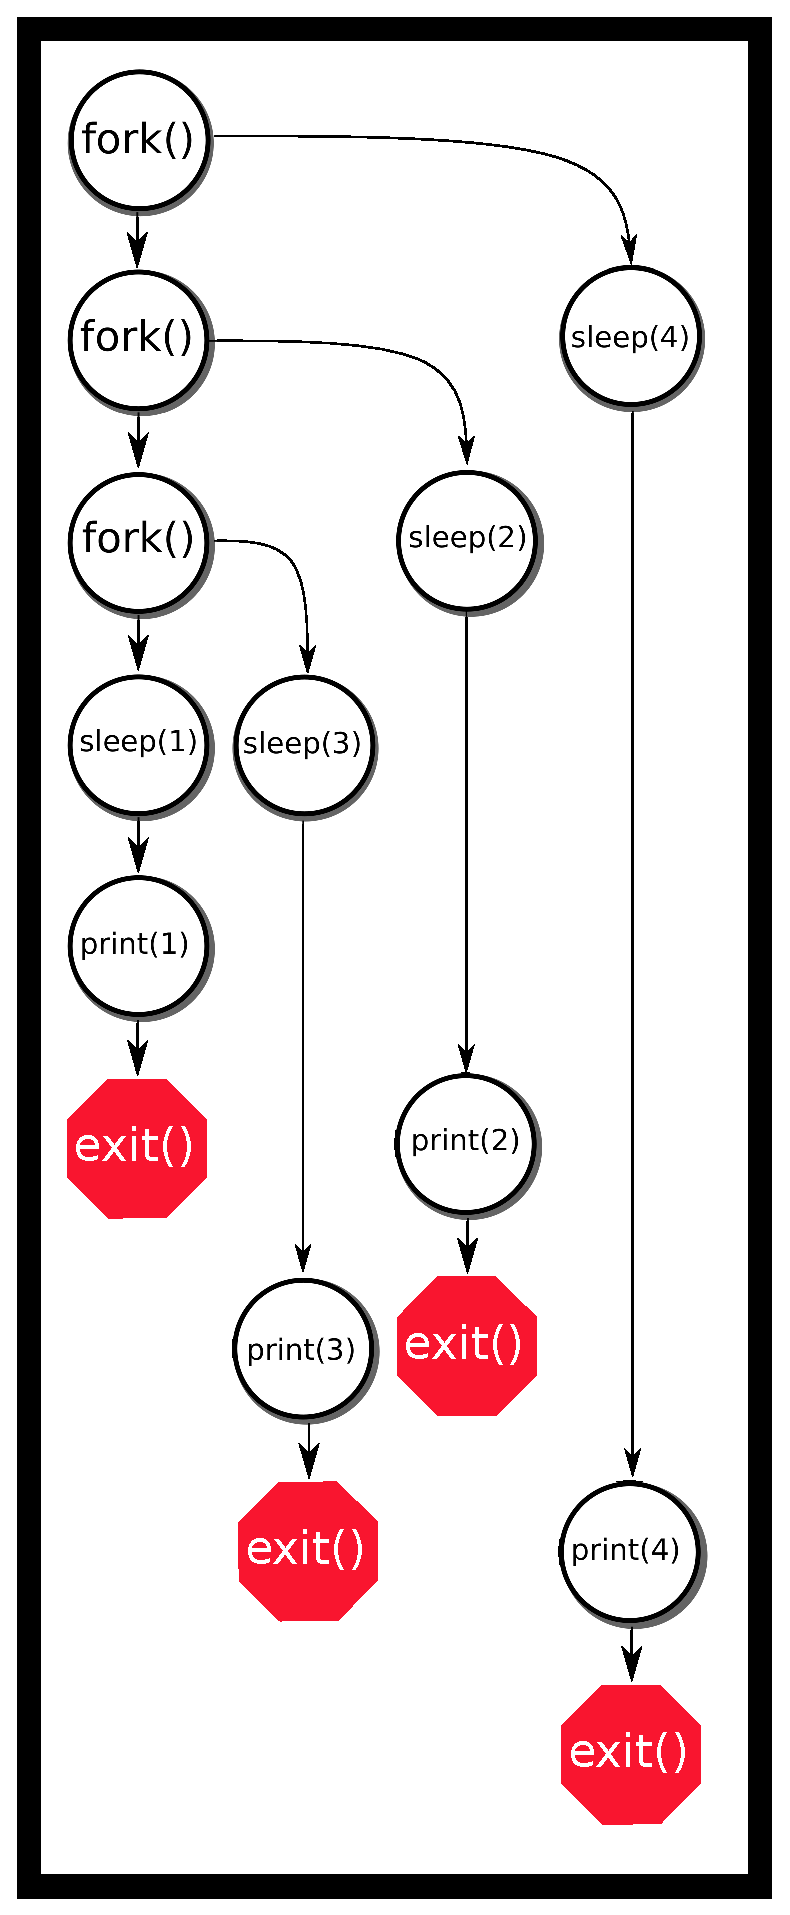
\includegraphics[width=.3\textwidth]{processes/drawings/sleepsort_timing.eps}
\caption{Timing of sorting 1, 3, 2, 4}
\end{figure}

The algorithm isn't actually O(N) because of how the system scheduler works.
In essence, this program outsources the actual sorting to the operating system.

\subsection{Fork Bomb}

A `fork bomb' is what we warned you about earlier.
This occurs when there is an attempt to create an infinite number of processes.
This will often bring a system to a near-standstill, as it attempts to allocate CPU time and memory to a very large number of processes that are ready to run.
System administrators don't like them and may set upper limits on the number of processes each user can have, or revoke login rights because they create disturbances in the Force for other users' programs.
A program can limit the number of child processes created by using \keyword{setrlimit()}.

Fork bombs are not necessarily malicious - they occasionally occur due to programming errors.
Below is a simple example that is malicious.

\begin{lstlisting}[language=C]
while (1) fork();
\end{lstlisting}

It is easy to cause one, if you are careless while calling fork, especially in a loop.
Can you spot the fork bomb here?

\begin{lstlisting}[language=C]
#include <unistd.h>
#define HELLO_NUMBER 10

int main(){
  pid_t children[HELLO_NUMBER];
  int i;
  for(i = 0; i < HELLO_NUMBER; i++){
    pid_t child = fork();
    if(child == -1) {
      break;
    }
    if(child == 0) {
      // Child
      execlp("ehco", "echo", "hello", NULL);
    }
    else{
      // Parent
      children[i] = child;
    }
  }

  int j;
  for(j = 0; j < i; j++){
    waitpid(children[j], NULL, 0);
  }
  return 0;
}
\end{lstlisting}

We misspelled \keyword{ehco}, so the \keyword{exec} call fails.
What does this mean? Instead of creating 10 processes, we just created \emph{1024 processes, fork bombing our machine}. \textbf{How could we prevent this? Add an exit right after exec, so that if exec fails, we won't end up calling fork an unbounded number of times.}
There are various other ways. What if we removed the \keyword{echo} binary? What if the binary itself creates a fork bomb?

\subsection{Signals}

We won't fully explore signals until the very end of the course, but it is relevant to broach the subject now because various semantics related to fork and other function calls detail what a signal is.

A signal can be thought of as a software interrupt. This means that a process that receives a signal stops the execution of the current program and makes the program respond to the signal.

There are various signals defined by the operating system, two of which you may already know: SIGSEGV and SIGINT.
The first is caused by an illegal memory access, and the second is sent by a user wanting to terminate a program.
In each case, the program jumps from the current line being executed to the signal handler.
If no signal handler is supplied by the program, a default handler is executed -- such as terminating the program, or ignoring the signal.

Here is an example of a simple user-defined signal handler:

\begin{lstlisting}[language=C]
void handler(int signum) {
  write(1, "signaled!", 9);
  // we don't need the signum because we are only catching SIGINT
  // if you want to use the same piece of code for multiple
  // signals, check the signum
}
int main() {
  signal(SIGINT, handler);
  while(1) ;
  return 0;
}
\end{lstlisting}

A signal has four stages in its life cycle: generated, pending, blocked, and received state.
These refer to when a process generates a signal, the kernel is about to deliver a signal, the signal is blocked, and when the kernel delivers a signal, each of which requires some time to complete.
Read more in the introduction to the Signals chapter.

The terminology is important because fork and exec require different operations based on the state a signal is in.

To note, it is generally poor programming practice to use signals in program logic, which is to send a signal to perform a certain operation.
The reason: signals have no time frame of delivery and no assurance that they will be delivered.
There are better ways to communicate between two processes.

If you want to read more, feel free to skip ahead to the chapter on POSIX signals and read it over. It isn't very long and gives you the long and short about how to deal with signals in processes.

\subsection{POSIX Fork Details}

POSIX determines the standards of fork \cite{fork_2018}.
You can read the previous citation, but do note that it can be quite verbose.
Here is a summary of what is relevant:

\begin{enumerate}
    \item Fork will return a non-negative integer on success.
    \item A child will inherit any open file descriptors of the parent.
          That means if a parent half of the file and forks, the child will start at that offset.
          A read on the child's end will shift the parent's offset by the same amount.
          Any other flags are also carried over.
    \item Pending signals are not inherited.
          This means that if a parent has a pending signal and creates a child, the child will not receive that signal unless another process signals the child.
    \item The process will be created with one thread (more on that later. The general consensus is to not create processes and threads at the same time).
    \item Since we have copy on write (COW), read-only memory addresses are shared between processes.
    \item If a program sets up certain regions of memory, they can be shared between processes.
    \item Signal handlers are inherited but can be changed.
    \item The process' current working directory (often abbreviated to CWD) is inherited but can be changed.
    \item Environment variables are inherited but can be changed.
\end{enumerate}

Key differences between the parent and the child include:
\begin{itemize}
    \item The process id returned by \keyword{getpid()}.
          The parent process id returned by \keyword{getppid()}.
    \item The parent is notified via a signal, SIGCHLD, when the child process finishes but not vice versa.
    \item The child does not inherit pending signals or timer alarms.
          For a complete list see the \href{http://man7.org/linux/man-pages/man2/fork.2.html}{fork man page}
    \item The child has its own set of environment variables.
\end{itemize}

\subsection{Fork and FILEs}

There are some tricky edge cases when it comes to using \keyword{FILE} and forking.
First, we have to make a technical distinction.
A \textbf{File Description} is the struct that a file descriptor points to.
File descriptors can point to many different structs, but for our purposes, they'll point to a struct that represents a file on a filesystem.
This file description contains elements like paths, how far the descriptor has read into the file, etc.
A file descriptor points to a file description.
This is important because when a process is forked, only the file descriptor is cloned, not the description.
The following snippet contains only one description.

\begin{lstlisting}[language=C]
  int file = open(...);
  if(!fork) {
    read(file, ...);
  } else {
    read(file, ...);
  }
\end{lstlisting}

One process will read one part of the file, the other process will read another part of the file.
In the following example, there are two descriptions caused by two different file handles.

\begin{lstlisting}[language=C]
  if(!fork) {
    int file = open(...);
    read(file, ...);
  } else {
    int file = open(...);
    read(file, ...);
  }
\end{lstlisting}

Let's consider our motivating example.

\begin{lstlisting}[language=bash]
$ cat test.txt
A
B
C
\end{lstlisting}

Take a look at this code, what does it do?

\begin{lstlisting}[language=C]
size_t buffer_cap = 0;
char * buffer = NULL;
ssize_t nread;
FILE * file = fopen("test.txt", "r");
int count = 0;
while((nread = getline(&buffer, &buffer_cap, file) != -1) {
  printf("%s", buffer);
  if(fork() == 0) { 
    exit(0);
  }
  wait(NULL);
}
\end{lstlisting}

The initial thought may be that it prints the file line by line with some extra forking.
It is actually undefined behavior because we didn't prepare the file descriptors.

To parse the \href{http://pubs.opengroup.org/onlinepubs/9699919799.2008edition/functions/V2_chap02.html}{POSIX documentation}, we'll have to go deep into the terminology.
The sentence that sets the expectation is the following

\begin{quote}
The result of function calls involving any one handle (the "active handle") is defined elsewhere in this volume of POSIX.1-2008, but if two or more handles are used, and any one of them is a stream, the application shall ensure that their actions are coordinated as described below. If this is not done, the result is undefined.
\end{quote}

What this means is that if we don't follow POSIX to the letter when using two file descriptors that refer to the same description across processes, we get undefined behavior.
To be technical, the file descriptor must have a ``position'' meaning that it needs to have a beginning and an end like a file, not like an arbitrary stream of bytes.
POSIX then goes on to introduce the idea of an active handle, where a handle may be a file descriptor or a \keyword{FILE*} pointer.
File handles don't have a flag called ``active''.
An active file descriptor is one that is currently being used for reading and writing and other operations (such as \keyword{exit}).
The standard says that before a \keyword{fork} that the \textit{application} or your code must execute a series of steps to prepare the state of the file.
In simplified terms, the descriptor needs to be closed, flushed, or read to its entirety -- the gory details are explained later.

\begin{quote}
For a handle to become the active handle, the application shall ensure that the actions below are performed between the last use of the handle (the current active handle) and the first use of the second handle (the future active handle). The second handle then becomes the active handle. All activity by the application affecting the file offset on the first handle shall be suspended until it again becomes the active file handle. (If a stream function has as an underlying function one that affects the file offset, the stream function shall be considered to affect the file offset.)
\end{quote}

Summarizing as if two file descriptors are actively being used, the behavior is undefined.
The other note is that after a fork, the library code must prepare the file descriptor as if the other process were to make the file active at any time.
The last bullet point concerns itself with how a process prepares a file descriptor in our case.

\begin{quote}
If the stream is open with a mode that allows reading and the underlying open file description refers to a device that is capable of seeking, the application shall either perform an fflush(), or the stream shall be closed.
\end{quote}

The documentation says that the child needs to perform an fflush or close the stream because the file descriptor needs to be prepared in case the parent process needs to make it active.
glibc is in a no-win situation if it closes a file descriptor that the parent may expect to be open, so it'll opt for the fflush on exit because exit in POSIX terminology counts as accessing a file.
That means that for our parent process, this clause gets triggered.

\begin{quote}
If any previous active handle has been used by a function that explicitly changed the file offset, except as required above for the first handle, the application shall perform an lseek() or fseek() (as appropriate to the type of handle) to an appropriate location.
\end{quote}

Since the child calls fflush and the parent didn't prepare, the operating system chooses to where the file gets reset.
Different file systems will do different things which are supported by the standard.
The OS may look at modification times and conclude that the file hasn't changed so no resets are needed or may conclude that exit denotes a change and needs to rewind the file back to the beginning.

What should you take away from this long-winded example to avoid undefined behavior?

\begin{enumerate}
\item You as the programmer need to make sure that all of your file descriptors are prepared before forking.
\item If it is a file descriptor or an unbuffered \keyword{FILE*}, it is already prepared.
\item If the \keyword{FILE*} is open for reading and has been read fully, it is already prepared.
\item Otherwise, the \keyword{FILE*} \textbf{must} be \keyword{fflush}'ed or closed to be prepared.
\item If the file descriptor is prepared, it must not be active in the parent process if the child process is using it or vice versa. A process is using it if it is read or written or if that process \textit{for whatever reason} calls \keyword{exit}. If a process uses it when the other process is as well, the whole application's behavior is undefined.
\end{enumerate}

So how would we fix the code?
We'd just have to flush the file before forking and refrain from using it until after the \keyword{wait} call -- more on the specifics of this next section.

\begin{lstlisting}[language=C]
size_t buffer_cap = 0;
char * buffer = NULL;
ssize_t nread;
FILE * file = fopen("test.txt", "r");
int count = 0;
while((nread = getline(&buffer, &buffer_cap, file) != -1) {
  printf("%s", buffer);
  fflush(file);
  if(fork() == 0) { 
    exit(0);
  }
  wait(NULL);
}
\end{lstlisting}

What if the parent process and the child process need to perform asynchronously and need to keep the file handle open?
Due to event ordering, we need to make sure that parent process knows that the child is finished using \keyword{wait}.
We'll talk about Inter-Process communication in a later chapter, but now we can use the double fork method.

\begin{lstlisting}[language=C]
//... 
fflush(file);
pid_t child = fork();
if(child == 0) { 
  fclose(file);
  if (fork() == 0) {
    // Do asynchronous work
    // Safe exit, this child doesn't know about
    // the file descriptor
    exit(0);
  }
  exit(0);
}
waitpid(child, NULL, 0);
\end{lstlisting}

\section{Waiting and Executing}

If the parent process wants to wait for the child to finish, it must use \keyword{waitpid} (or \keyword{wait}), both of which wait for a child to change process states, which can be one of the following:

\begin{enumerate}
\item The child terminated
\item The child was stopped by a signal
\item The child was resumed by a signal
\end{enumerate}

Note that waitpid can be set to be non-blocking, which means they will return immediately, letting a program know if the child has exited.

\begin{lstlisting}[language=C]
pid_t child_id = fork();
if (child_id == -1) { perror("fork"); exit(EXIT_FAILURE);}
if (child_id > 0) {
  // We have a child! Get their exit code
  int status;
  waitpid( child_id, &status, 0 );
  // code not shown to get exit status from child
} else { // In child ...
  // start calculation
  exit(123);
}
\end{lstlisting}

\keyword{wait} is a simpler version of \keyword{waitpid}.
\keyword{wait} accepts a pointer to an integer and waits on any child process.
After the first one changes state, \keyword{wait} returns.
Here is the behavior of \keyword{waitpid}:

\begin{enumerate}
\item A program \emph{can} wait on a specific process, or it can pass in special values for the \keyword{pid} to do different things (check the man pages).
\item The last parameter to waitpid is an option parameter.
The options are listed below:
  \begin{enunmerate}
      \item WNOHANG - Return whether or not the searched process has exited
      \item WNOWAIT - Wait, but leave the child wait-able by another wait call
      \item WEXITED - Wait for exited children
      \item WSTOPPED - Wait for stopped children
      \item WCONTINUED - Wait for continued children
  \end{enunmerate}
\end{enumerate}

Exit statuses or the value stored in the integer pointer for both of the calls above are explained below.

\subsection{Exit statuses}

To find the return value of \keyword{main()} or value included in \keyword{exit()}), Use the \keyword{Wait macros} - typically a program will use \keyword{WIFEXITED} and \keyword{WEXITSTATUS} .
See \keyword{wait}/\keyword{waitpid} man page for more information.

\begin{lstlisting}[language=C]
int status;
pid_t child = fork();
if (child == -1) {
  return 1; //Failed
}
if (child > 0) {
  // Parent, wait for child to finish
  pid_t pid = waitpid(child, &status, 0);
  if (pid != -1 && WIFEXITED(status)) {
    int exit_status = WEXITSTATUS(status);
    printf("Process %d returned %d" , pid, exit_status);
  }
} else {
  // Child, do something interesting
  execl("/bin/ls", "/bin/ls", ".", (char *) NULL); // "ls ."
}
\end{lstlisting}

A process can only have 256 return values, the rest of the bits are informational, and the information is extracted with bit shifting.
However, the kernel has an internal way of keeping track of signaled, exited, or stopped processes.
This API is abstracted so that that the kernel developers are free to change it at will.
Remember: these macros only make sense if the precondition is met.
For example, a process' exit status won't be defined if the process isn't signaled.
The macros will not do the checking for the program, so it's up to the programmer to make sure the logic is correct.
As an example above, the program should use the \keyword{WIFSTOPPED} to check if a process was stopped and then the \keyword{WSTOPSIG} to find the signal that stopped it.
As such, there is no need to memorize the following. This is just a high-level overview of how information is stored inside the status variables. From the \keyword{sys/wait.h} of an old Berkeley Standard Distribution(BSD) kernel \cite{sys/wait.h}:

\begin{lstlisting}[language=C]
/* If WIFEXITED(STATUS), the low-order 8 bits of the status. */
#define _WSTATUS(x) (_W_INT(x) & 0177)
#define _WSTOPPED 0177    /* _WSTATUS if process is stopped */
#define WIFSTOPPED(x) (_WSTATUS(x) == _WSTOPPED)
#define WSTOPSIG(x) (_W_INT(x) >> 8)
#define WIFSIGNALED(x)  (_WSTATUS(x) != _WSTOPPED && _WSTATUS(x) != 0)
#define WTERMSIG(x) (_WSTATUS(x))
#define WIFEXITED(x)  (_WSTATUS(x) == 0)
\end{lstlisting}

There is a convention about exit codes.
If the process exited normally and everything was successful, then a zero should be returned.
Beyond that, there aren't too many widely accepted conventions.
If a program specifies return codes to mean certain conditions, it may be able to make more sense of the 256 error codes.
For example, a program could return \keyword{1} if the program went to stage 1 (like writing to a file) \keyword{2} if it did something else, etc.
Usually, UNIX programs are not designed to follow this policy, for the sake of simplicity.


\subsection{Zombies and Orphans}

It is good practice to wait on your process' children.
If a parent doesn't wait on your children they become, what are called zombies.
Zombies are created when a child terminates and then takes up a spot in the kernel process table for your process.
The process table keeps track of the following information about a process: PID, status, and how it was killed.
The only way to get rid of a zombie is to wait on your children.
If a long-running parent never waits for your children, it may lose the ability to fork.

Having said that, a program doesn't always need to wait for your children!
Your parent process can continue to execute code without having to wait for the child process.
If a parent dies without waiting on its children, a process can orphan its children.
Once a parent process completes, any of its children will be assigned to \keyword{init} - the first process, whose PID is 1.
Therefore, these children would see \keyword{getppid()} return a value of 1.
These orphans will eventually finish and for a brief moment become a zombie.
The init process automatically waits for all of its children, thus removing these zombies from the system.

\subsection{Extra: Asynchronously Waiting}

Warning: This section uses signals which we have not yet fully introduced.
The parent gets the signal SIGCHLD when a child completes, so the signal handler can wait for the process.
A slightly simplified version is shown below.

\begin{lstlisting}[language=C]
pid_t child;

void cleanup(int signal) {
  int status;
  waitpid(child, &status, 0);
  write(1,"cleanup!\n",9);
}
int main() {
  // Register signal handler BEFORE the child can finish
  signal(SIGCHLD, cleanup); // or better - sigaction
  child = fork();
  if (child == -1) { exit(EXIT_FAILURE);}

  if (child == 0) {
    // Do background stuff e.g. call exec
  } else { /* I'm the parent! */
    sleep(4); // so we can see the cleanup
    puts("Parent is done");
  }
  return 0;
}
\end{lstlisting}

However, the above example misses a couple of subtle points.
\begin{enumerate}
    \item More than one child may have finished but the parent will only get one SIGCHLD signal (signals are not queued)
    \item SIGCHLD signals can be sent for other reasons (e.g. a child process has temporarily stopped)
    \item It uses the deprecated \keyword{signal} code, instead of the more portable sigaction.
\end{enumerate}

A more robust code to reap zombies is shown below.

\begin{lstlisting}[language=C]
void cleanup(int signal) {
  int status;
  while (waitpid((pid_t) (-1), 0, WNOHANG) > 0) {

  }
}
\end{lstlisting}

\section{exec}

To make the child process execute another program, use one of the \href{http://man7.org/linux/man-pages/man3/exec.3.html}{\keyword{exec}} functions after forking.
The \keyword{exec} set of functions replaces the process image with that of the specified program.
This means that any lines of code after the \keyword{exec} call are replaced with those of the executed program.
Any other work a program wants the child process to do should be done before the \keyword{exec} call.
The naming schemes can be shortened mnemonically.

\begin{enumerate}
    \item e -- An array of pointers to environment variables is explicitly passed to the new process image.
    \item l -- Command-line arguments are passed individually (a list) to the function.
    \item p -- Uses the PATH environment variable to find the file named in the file argument to be executed.
    \item v -- Command-line arguments are passed to the function as an array (vector) of pointers.
\end{enumerate}

Note that if the information is passed via an array, the last element must be followed by a NULL element to terminate the array.

An example of this code is below. This code executes \keyword{ls}

\begin{lstlisting}[language=C]
#include <unistd.h>
#include <sys/types.h>
#include <sys/wait.h>
#include <stdlib.h>
#include <stdio.h>

int main(int argc, char**argv) {
  pid_t child = fork();
  if (child == -1) return EXIT_FAILURE;
  if (child) {
    int status;
    waitpid(child , &status ,0);
    return EXIT_SUCCESS;

  } else {
    // Other versions of exec pass in arguments as arrays
    // Remember first arg is the program name
    // Last arg must be a char pointer to NULL

    execl("/bin/ls", "/bin/ls", "-alh", (char *) NULL);

    // If we get to this line, something went wrong!
    perror("exec failed!");
  }
}
\end{lstlisting}

Try to decode the following example

\begin{lstlisting}[language=C]
#include <unistd.h>
#include <fcntl.h> // O_CREAT, O_APPEND etc. defined here

int main() {
  close(1); // close standard out
  open("log.txt", O_RDWR | O_CREAT | O_APPEND, S_IRUSR | S_IWUSR);
  puts("Captain's log");
  chdir("/usr/include");
  // execl( executable,  arguments for executable including program name and NULL at the end)

  execl("/bin/ls", /* Remaining items sent to ls*/ "/bin/ls", ".", (char *) NULL); // "ls ."
  perror("exec failed");
  return 0;
}
\end{lstlisting}

The example writes "Captain's Log" to a file then prints everything in /usr/include to the same file.
There's no error checking in the above code (we assume close, open, chdir etc. work as expected).

\begin{enumerate}
    \item \keyword{open} -- will use the lowest available file descriptor (i.e. 1) ; so standard out(stdout) is now redirected to the log file.
    \item \keyword{chdir} -- Change the current directory to /usr/include
    \item \keyword{execl} -- Replace the program image with /bin/ls and call its main() method
    \item \keyword{perror} -- We don't expect to get here - if we did then \keyword{exec} failed.
    \item We need the "return 0;" because compilers complain if we don't have it.
\end{enumerate}

\subsection{POSIX Exec Details}

POSIX details all of the semantics that exec needs to cover \cite{exec_2018}.
Note the following

\begin{enumerate}
\item File descriptors are preserved after an exec. That means if a program open a file and doesn't to close it, it remains open in the child.
  This is a problem because usually the child doesn't know about those file descriptors. Nevertheless, they take up a slot in the file descriptor table and could possibly prevent other processes from accessing the file.
  The one exception to this is if the file descriptor has the Close-On-Exec flag set (O\_CLOEXEC) -- we will go over setting flags later.
\item Various signal semantics. The executed processes preserve the signal mask and the pending signal set but does not preserve the signal handlers since it is a different program.
\item Environment variables are preserved unless using an environ version of exec
\item The operating system may open up 0, 1, 2 -- stdin, stdout, stderr, if they are closed after exec, most of the time they leave them closed.
\item The executed process runs as the same PID and has the same parent and process group as the previous process.
\item The executed process is run on the same user and group with the same working directory
\end{enumerate}

\subsection{Shortcuts}

\keyword{system} pre-packs the above code \cite[P. 371]{jones2010wg14}.
The following is a snippet of how to use system.

\begin{lstlisting}[language=C]
#include <unistd.h>
#include <stdlib.h>

int main(int argc, char**argv) {
  system("ls"); // execl("/bin/sh", "/bin/sh", "-c", "\\"ls\\"")
  return 0;
}
\end{lstlisting}

The \keyword{system} call will fork, execute the command passed by parameter and the original parent process will wait for this to finish.
This also means that \keyword{system} is a blocking call.
The parent process can't continue until the process started by \keyword{system} exits.
Also, \keyword{system} actually creates a shell that is then given the string, which is more overhead than just using \keyword{exec} directly.
The standard shell will use the \keyword{PATH} environment variable to search for a filename that matches the command.
Using system will usually be sufficient for many simple run-this-command problems but can quickly become limiting for more complex or subtle problems, and it hides the mechanics of the fork-exec-wait pattern, so we encourage you to learn and use \keyword{fork} \keyword{exec} and \keyword{waitpid} instead.
It also tends to be a huge security risk.
By allowing someone to access a shell version of the environment, the program can run into all sorts of problems:

\begin{lstlisting}[language=C]
int main(int argc, char**argv) {
  char *to_exec = asprintf("ls %s", argv[1]);
  system(to_exec);
}
\end{lstlisting}

Passing something along the lines of argv[1] = "; sudo su" is a huge security risk called \href{https://en.wikipedia.org/wiki/Privilege\_escalation}{privilege escalation}.

\section{The fork-exec-wait Pattern}

A common programming pattern is to call \keyword{fork} followed by \keyword{exec} and \keyword{wait}.
The original process calls fork, which creates a child process.
The child process then uses exec to start the execution of a new program.
Meanwhile, the parent uses \keyword{wait} (or \keyword{waitpid}) to wait for the child process to finish.

\begin{figure}[H]
\centering
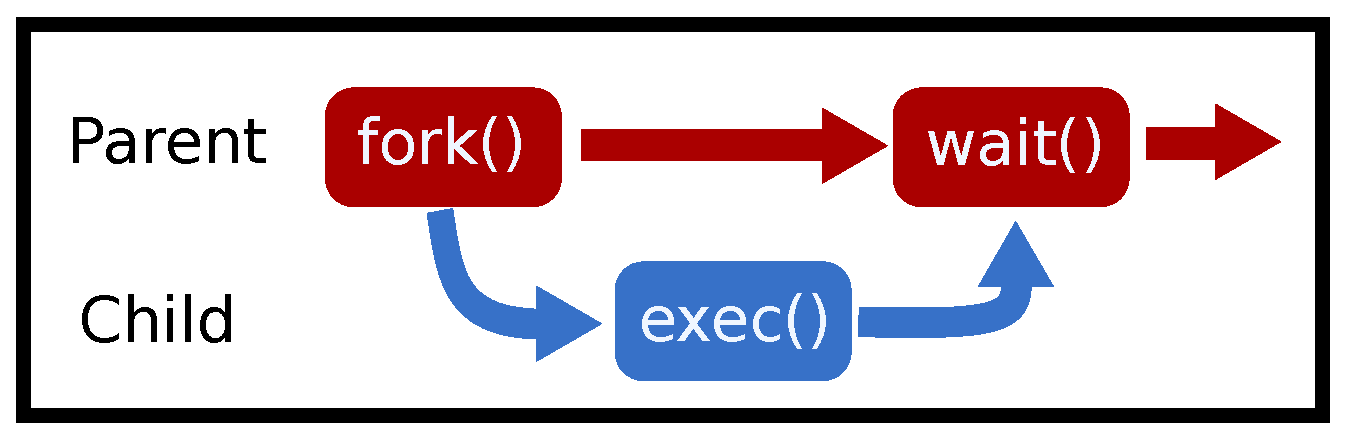
\includegraphics[width=.7\textwidth]{processes/drawings/fork_exec_wait.eps}
\caption{Fork, exec, wait diagram}
\end{figure}

\begin{lstlisting}[language=C][language=C]
#include <unistd.h>

int main() {
  pid_t pid = fork();
  if (pid < 0) { // fork failure
    exit(1);
  } else if (pid > 0) {
    int status;
    waitpid(pid, &status, 0);
  } else {
    execl("/bin/ls", "/bin/ls", NULL);
    exit(1); // For safety.
  }
}
\end{lstlisting}

Why not execute ls directly?
The reason is that now we have a monitor program -- our parent that can do other things.
It can proceed and execute another function, or it can also modify the state of the system or read the output of the function call.

\subsection{Environment Variables}

Environment variables are variables that the system keeps for all processes to use.
Your system has these set up right now!
In Bash, some are already defined

\begin{lstlisting}[language=bash]
$ echo $HOME
/home/bhuvy
$ echo $PATH
/usr/local/sbin:/usr/bin:...
\end{lstlisting}

How would a program later these in C?
They can call \keyword{getenv} and \keyword{setenv} function respectively.

\begin{lstlisting}[language=C]
char* home = getenv("HOME"); // Will return /home/bhuvy
setenv("HOME", "/home/bhuvan", 1 /*set overwrite to true*/ );
\end{lstlisting}

Environment variables are important because they are inherited between processes and can be used to specify a standard set of behaviors \cite{env_std_2018}, although you don't need to memorize the options.
Another security related concern is that environment variables cannot be read by an outside process, whereas argv can be.

\section{Further Reading}

Read the man pages and the POSIX groups above!
Here are some guiding questions.
Note that we aren't expecting you to memorize the man page.

\begin{itemize}
\item What is one reason fork may fail?
\item Does fork copy all pages to the child?
\item Are file descriptors cloned between parent and child?
\item Are file descript\textbf{ions} cloned between parent and child?
\item What is the difference between exec calls ending in an \keyword{e}?
\item What is the difference between l and v in an exec call? How about \keyword{p}?
\item When does exec error? What happens?
\item Does wait only notify if a child has exited?
\item Is it an error to pass a negative value into wait?
\item How does one extract information out of the status?
\item Why may wait fail?
\item What happens when a parent doesn't wait on their children?
\end{itemize}

\begin{itemize}
\item \href{http://man7.org/linux/man-pages/man2/fork.2.html}{fork}
\item \href{http://man7.org/linux/man-pages/man3/exec.3.html}{exec}
\item \href{http://man7.org/linux/man-pages/man2/wait.2.html}{wait}
\end{itemize}

\subsection{Topics}

\begin{itemize}
\item Correct use of fork, exec and waitpid
\item Using exec with a path
\item Understanding what fork and exec and waitpid do. E.g. how to use their return values.
\item SIGKILL vs SIGSTOP vs SIGINT.
\item What signal is sent when press CTRL-C at a terminal?
\item Using kill from the shell or the kill POSIX call.
\item Process memory isolation.
\item Process memory layout (where is the heap, stack etc; invalid memory addresses).
\item What is a fork bomb, zombie and orphan? How to create/remove them.
\item getpid vs getppid
\item How to use the WAIT exit status macros WIFEXITED etc.
\end{itemize}

\section{Questions/Exercises}

\begin{itemize}
    \item
          What is the difference between execs with a p and without a p? What does the operating system
    \item
          How does a program pass in command line arguments to \keyword{execl*}? How about \keyword{execv*}? What should be the first command line argument by convention?
    \item
          How does a program know if \keyword{exec} or \keyword{fork} failed?
    \item
          What is the \keyword{int\ *status} pointer passed into wait? When does wait fail?
    \item
          What are some differences between \keyword{SIGKILL}, \keyword{SIGSTOP}, \keyword{SIGCONT}, \keyword{SIGINT}? What are the default behaviors? Which ones can a program set up a signal handler for?
    \item
          What signal is sent when you press \keyword{CTRL-C}?
    \item
          My terminal is anchored to PID = 1337 and has just become unresponsive. Write me the terminal command and the C code to send \keyword{SIGQUIT} to it.
    \item
          Can one process alter another processes memory through normal means? Why?
    \item
          Where is the heap, stack, data, and text segment? Which segments can a program write to? What are invalid memory addresses?
    \item
          Code up a fork bomb in C (please don't run it).
    \item
          What is an orphan? How does it become a zombie? What should a parent do to avoid this?
    \item
      Don't you hate it when your parents tell you that you can't do something?
      Write a program that sends \keyword{SIGSTOP} to a parent process.
    \item
          Write a function that fork exec waits an executable, and using the wait macros tells me if the process exited normally or if it was signaled. If the process exited normally, then print that with the return value. If not, then print the signal number that caused the process to terminate.
\end{itemize}

\bibliographystyle{plainnat}
\bibliography{processes/processes}

%\chapter{Memory Allocators}

\epigraph{Memory memory everywhere but not a allocation to be made}{A really fragmented heap}

\section{Introduction}

Memory allocation is very important!
Allocating and de-allocating heap memory is one of the most common operations in any application.
The heap at the system level is contiguous series of addresses that the program can expand or contract and use as its own accord \cite{mallocinternals}.
In POSIX, this is called the system break.
We use \keyword{sbrk} to move the system break.
Most programs don't interact directly with this call, they use a memory allocation system around it to handle chunking up and keeping track of which memory is allocated and which is freed.

We will mainly be looking into simple allocators.
Just know that there are other ways of dividing up memory like with \texttt{mmap} or other allocation schemes and methods like \keyword{jemalloc}.

\section{C Memory Allocation API}

\begin{itemize}

\item \keyword{malloc(size\_t bytes)} is a C library call and is used to reserve a contiguous block of memory that may be uninitialized \cite[P. 348]{jones2010wg14}.
Unlike stack memory, the memory remains allocated until \keyword{free} is called with the same pointer.
If \keyword{malloc} can either return a pointer to at least that much free space requested or \texttt{NULL}.
That means that malloc can return NULL even if there is some spaces.
Robust programs should check the return value.
If your code assumes \keyword{malloc} succeeds, and it does not, then your program will likely crash (segfault) when it tries to write to address 0.
Also, malloc may not zero out memory because of performance -- check your code to make sure that you are not using uninitialized values.

\item \keyword{realloc(void *space, size\_t bytes)} allows you to resize an existing memory allocation that was previously allocated on the heap (via malloc, calloc, or realloc) \cite[P. 349]{jones2010wg14}.
The most common use of realloc is to resize memory used to hold an array of values.
There are two gotchas with realloc.
One, a new pointer may be returned.
Two, it can fail.
A naive but readable version of realloc is suggested below with sample usage.

\begin{lstlisting}[language=C]
void * realloc(void * ptr, size_t newsize) {
  // Simple implementation always reserves more memory
  // and has no error checking
  void *result = malloc(newsize);
  size_t oldsize =  ... //(depends on allocator's internal data structure)
  if (ptr) memcpy(result, ptr, newsize < oldsize ? newsize : oldsize);
  free(ptr);
  return result;
}

int main() {
  // 1
  int *array = malloc(sizeof(int) * 2);
  array[0] = 10; array[1] = 20;
  // Oops need a bigger array - so use realloc..
  array = realloc(array, 3 * sizeof(int));
  array[2] = 30;

}
\end{lstlisting}

The above code is not robust.
If \keyword{realloc} fails then the array is a memory leak.
Robust code checks for the return value and only reassigns the original pointer if not null.

\begin{lstlisting}[language=C]
int main() {
  // 1
  int *array = malloc(sizeof(int) * 2);
  array[0] = 10; array[1] = 20;
  void *tmp = realloc(array, 3 * sizeof(int));
  if (tmp == NULL) {
    // Nothing I can do here
  } else if (tmp == array) {
    // realloc returned same space
    array[2] = 30;
  } else {
    // realloc returned different space
    array = tmp;
    array[2] = 30;
  }

}
\end{lstlisting}

\item \keyword{calloc(size\_t nmemb, size\_t size)} initializes memory contents to zero and also takes two arguments: the number of items and the size in bytes of each item.
An advanced discussion of these limitations is \href{http://locklessinc.com/articles/calloc/}{in this article}.
Programmers often use \keyword{calloc} rather than explicitly calling \keyword{memset} after \keyword{malloc}, to set the memory contents to zero because certain performance considerations are taken into account.
Note \keyword{calloc(x,y)} is identical to \keyword{calloc(y,x)}, but you should follow the conventions of the manual.
A naive implementation of calloc is below.

\begin{lstlisting}[language=C]
void *calloc(size_t n, size_t size) {
  size_t total = n * size; // Does not check for overflow!
  void *result = malloc(total);

  if (!result) return NULL;

  // If we're using new memory pages
  // just allocated from the system by calling sbrk
  // then they will be zero so zero-ing out is unnecessary,
  // We will be non-robust and memset either way.
  return memset(result, 0, total);
}
\end{lstlisting}

\item \keyword{free} takes a pointer to the start of a piece of memory and makes it available for use in the subsequent calls to the other allocation functions.
This is important because we don't want every process in our address space to take an enormous amount of memory.
Once we are done using memory, we stop using it with free.
A simple usage is below.

\begin{lstlisting}[language=C]
int *ptr = malloc(sizeof(*ptr));
do_something(ptr);
free(ptr);
\end{lstlisting}

If you use a piece of memory after it is freed - that is undefined behavior.

\end{itemize}

\subsection{Heaps and sbrk}

The heap is part of the process memory, and it does not have a fixed size.
Heap memory allocation is performed by the C library when you call \keyword{malloc} (\keyword{calloc}, \keyword{realloc}) and \keyword{free}.
By calling \keyword{sbrk} the C library can increase the size of the heap as your program demands more heap memory.
As the heap and stack need to grow, we put them at opposite ends of the address space.
Stacks don't grow like a heap, new parts of the stack are allocated for new threads.
So for typical architectures the heap will grow upwards and the stack grows downwards.

Nowadays, Modern operating system memory allocators no longer need \keyword{sbrk} - instead they can request independent regions of virtual memory and maintain multiple memory regions.
For example, gibibyte requests may be placed in a different memory region than small allocation requests.
However this detail is an unwanted complexity.

Programs don't need to call \texttt{brk} or \texttt{sbrk} typically, though calling \keyword{sbrk(0)} can be interesting because it tells you where your heap currently ends.
Instead programs use \keyword{malloc},\keyword{calloc},\keyword{realloc} and \keyword{free} which are part of the C library.
The internal implementation of these functions may call \keyword{sbrk} when additional heap memory is required.

\begin{lstlisting}[language=C]
void *top_of_heap = sbrk(0);
malloc(16384);
void *top_of_heap2 = sbrk(0);
printf("The top of heap went from %p to %p \n", top_of_heap, top_of_heap2);
// Example output: The top of heap went from 0x4000 to 0xa000
\end{lstlisting}

An important fact we just glossed over earlier is memory that was newly obtained by the operating system must be zeroed out.
If the operating system did not zero out contents of physical RAM, it might be possible for one process to learn about the memory of another process that had previously used the memory.
This would be a security leak.
Unfortunately this means that for \keyword{malloc} requests before any memory has been freed is \emph{often} zero.
This is unfortunate because, many programmers mistaken write C programs that assume malloc'd memory will \emph{always} be zero.

\begin{lstlisting}[language=C]
char* ptr = malloc(300);
// contents is probably zero because we get brand new memory
// so beginner programs appear to work!
// strcpy(ptr, "Some data"); // work with the data
free(ptr);
// later
char *ptr2 = malloc(300); // Contents might now contain existing data and is probably not zero
\end{lstlisting}

\section{Intro to Allocating}

Let's try to write Malloc.
Here is a first attempt at it -- the naive version.

\begin{lstlisting}[language=C]
void* malloc(size_t size)
// Ask the system for more bytes by extending the heap space.
// sbrk Returns -1 on failure
   void *p = sbrk(size);
   if(p == (void *) -1) return NULL; // No space left
   return p;
}
void free() {/* Do nothing */}
\end{lstlisting}

Above is the simplest implementation of malloc, there are a few drawbacks though.

\begin{itemize}
\item System calls are slow compared to library calls.
  We should reserve a large amount of memory and only occasionally ask for more from the system.
\item No reuse of freed memory.
  Our program never re-uses heap memory - it just keeps asking for a bigger heap.
\end{itemize}

If this allocator was used in a typical program, the process would quickly exhaust all available memory.
Instead we need an allocator that can efficiently use heap space and only ask for more memory when necessary.
There are programs that may use this type of allocator.
Consider a video game allocating objects to load the next scene.
It is considerably faster to do the above and just throw the entire block of memory away than it is to do the following placement strategies.

\subsection{Placement Strategies}

During program execution, memory is allocated and de-allocated, so there will be gap in the heap memory that can be re-used for future memory requests.
The memory allocator needs to keep track of which parts of the heap are currently allocated and which are parts are available.
Suppose our current heap size is 64K, though not all of it is in use because some earlier malloc'd memory has already been freed by the program.
Let's say that our heap looks like the following table.
\\
\begin{center}
\begin{tabular}{ | c | c | c | c | c | c | c | }
\hline
16KiB & 10KiB & 1KiB & 1KiB & 30KiB & 4KiB & 2KiB \\ \hline
free & allocated & free & allocated & free & allocated & free \\
\hline
\end{tabular}
\end{center}
\\
If a new malloc request for 2KiB is executed (\keyword{malloc(2048)}), where should \keyword{malloc} reserve the memory?
It could use the last 2KiB hole, which happens to be the perfect size!
Or it could split one of the other two free holes.
These choices represent different placement strategies.
Whichever hole is chosen, the allocator will need to split the hole into two.
The newly allocated space, which will be returned to the program and a smaller hole if there is spare space left over.
A perfect-fit strategy finds the smallest hole that is of sufficient size (at least 2KiB):
\\
\begin{center}
\begin{tabular}{ | c | c | c | c | c | c | c | }
\hline
16KiB & 10KiB & 1KiB & 1KiB & 30KiB & 4KiB & 2KiB \\ \hline
free & allocated & free & allocated & free & allocated & \texttt{HERE!} \\
\hline
\end{tabular}
\end{center}
\\
A worst-fit strategy finds the largest hole that is of sufficient size so break the 30KiB hole into two:
\\
\begin{center}
\begin{tabular}{ | c | c | c | c | c | c | c | c | }
\hline
16KiB & 10KiB & 1KiB & 1KiB & 2KiB & 28KiB & 4KiB & 2KiB \\ \hline
free & allocated & free & allocated & \texttt{HERE!} & free & allocated & free \\
\hline
\end{tabular}
\end{center}
\\
A first-fit strategy finds the first available hole that is of sufficient size so break the 16KiB hole into two:
\\
\begin{center}
\begin{tabular}{ | c | c | c | c | c | c | c | c | }
\hline
2KiB & 14KiB & 10KiB & 1KiB & 1KiB & 30KiB & 4KiB & 2KiB \\ \hline
\texttt{HERE!} & free & allocated & free & allocated & free & allocated & free \\
\hline
\end{tabular}
\end{center}
\\

To introduce another concept, external fragmentation is that even though we have enough memory in the heap, it may be divided up in a way that wear are not able to give the full amount.
In the example below, of the 64KiB of heap memory, 17KiB is allocated, and 47KiB is free.
However the largest available block is only 30KiB because our available unallocated heap memory is fragmented into smaller pieces.
\\
\begin{center}
\begin{tabular}{ | c | c | c | c | c | c | c | }
\hline
16KiB & 10KiB & 1KiB & 1KiB & 30KiB & 4KiB & 2KiB \\ \hline
free & allocated & free & allocated & free & allocated & free \\
\hline
\end{tabular}
\end{center}
\\

\subsection{Placement Strategy pros and cons}

The challenges of writing a heap allocator are
\begin{itemize}
\item Need to minimize fragmentation (i.e.~maximize memory utilization)
\item Need high performance
\item Fiddly implementation -- lots of pointer manipulation using linked lists and pointer arithmetic.
\item Both fragmentation and performance depend on the application allocation profile, which can be evaluated but not predicted and in practice, under-specific usage conditions, a special-purpose allocator can often out-perform a general purpose implementation.
\item The allocator doesn't know the program's memory allocation requests in advance. Even if we did, this is the \href{http://en.wikipedia.org/wiki/Knapsack_problem}{Knapsack problem} which is known to be NP hard!
\end{itemize}

Different strategies affect the fragmentation of heap memory in non-obvious ways, which only are discovered by mathematical analysis or careful simulations under real-world conditions (for example simulating the memory allocation requests of a database or web server).


First we will have a more mathematical, one-shot approach to each of these algorithms \cite{Garey:1972:WAM:800152.804907}. The paper describes a scenario where you have a certain number of bins, and a certain number of allocations, and you are trying to fit the allocations in as few bins as possible, hence using as little memory as possible.
The paper discusses theoretical implications and puts a nice limit on the ratios in the long run between the ideal memory usage and the actual memory usage.
For those who are interested, the paper concludes that actual memory usage over ideal memory usage as the number of bins increases -- the bins can have any distribution -- is about 1.7 for first fit and lower bounded by 1.7 for best fit.
The problem with this analysis is that very few real world applications need this type of one-shot allocation.
Video game object allocations will typically designate a different subheap for each level and fill up that subheap if they need a quick memory allocation scheme that they can throw away.

In practice, we'll be using the result from a more rigorous survey conducted in 2005 \cite{10.1007/3-540-60368-9_19}.
The paper makes sure to note that memory allocation is a moving target.
A good allocation scheme to one program may not be a good allocation scheme to another program.
Programs don't uniformly follow the distribution of allocations, so very.
The survey talks about all the allocation schemes that we have introduced as well as a few extra ones.
Here are some summarized takeaways

\begin{enumerate}
\item Best fit may have problems when a block is chosen that is almost the right size, and the remaining space is split so small that a program probably won't use it.
  A way to get around this could be to set a threshold for splitting.
  This small splitting isn't observed as frequently under regular work load.
  In addition, the worst case behavior of best fit is bad, but doesn't usually happen p. 43.
\item The paper also talks about an important distinction of first fit.
  There are multiple notions of first.
  First could be ordered in terms of time of free, or it could be ordered through the addresses of the start of the block, or it could be ordered by the time of last free -- first being least recently used.
  The survey didn't go too in depth into the performance of each, but did make a note that address ordered and least recently used lists ended up with better performance than the most recently used first.
\item The paper concludes by first saying that under simulated random (assuming uniform at random) work loads, best fit and first fit do as well. Even in practice, both best and address ordered first fit do about as equally as well with a splitting threshold and coalescing. The reasons why aren't entirely known.
\end{enumerate}

Some additional notes we make

\begin{enumerate}
\item Best fit may not require a full scan of the heap. When a block of perfect size or of perfect size within a threshold is found, that can be returned, depending on what edge-case policy you have.
\item Worst fit may not need to scan the entire heap as well. Depending on how you set up data structures, your heap could represent the data structure max-heap and each allocation call simply needs to pop the top off, reheapify, and possibly insert a split memory block.
  Using Fibonacci heaps, that can be extremely inefficient.
\item First fit needs to have some sort of ordering. Most of the time people will default to linked lists which is a fine choice. There isn't too many improvements you can make with a least recently used and most recently used linked list policy, but with address ordered linked lists you can speed up insertion from O(n) to O(log(n)) by using a randomized skip-list in conjunction with your singly linked list.
  Basically an insert would use the skip list as shortcuts to find the right place to insert the block and a removal would go through the list as normal.
\item There are many placement strategies that we haven't talked about, one is next-fit which is first fit on the next fit block. This adds a sort-of deterministic randomness. You won't be expected to know this algorithm, just know as you are implementing a memory allocator as part of a machine problem, there are more than these.
  \end{enumerate}

\section{Memory Allocator Tutorial}

A memory allocator needs to keep track of which bytes are currently allocated and which are available for use.
This section introduces the implementation and conceptual details of building an allocator, or the actual code that implements \keyword{malloc} and \keyword{free}.

Conceptually we are thinking about creating linked lists and lists of blocks!
Please enjoy the following ASCII art.
bt is short for boundary tag.

\begin{verbatim}
| I am one block  | I am another   | Tiny block  |
|-----------------|----------------|-------------|
| meta | space |bt| meta | space|bt| meta |spc|bt|
|-----------------|----------------|-------------|
\end{verbatim}

We will have implicit pointers in our next block, meaning that we can get from one block to another using addition.
This is in contrast to an explicit \texttt{metadata *next} field in our meta block.

\begin{verbatim}
|-----------------|
p                 |
|-----------------|----------------|-------------|
| meta | space |bt| meta | space|bt| meta |spc|bt|
|-----------------|----------------|-------------|

If p is char pointer to the start of our block, to get to the next block would be

p + sizeof(meta) + p->space + sizeof(boundary_tag)
\end{verbatim}

The actual spacing may be different.
The metadata can contain different things.
A minimal metadata would simply have the size of the block.

Since we write integers and pointers into memory that we already control, we can later consistently hop from one address to the next.
This internal information represents some overhead.
Meaning even if we had requested 1024 KiB of contiguous memory from the system, we will not be able to provide all of it to the running program.

Our heap memory is a list of blocks where each block is either allocated or unallocated.
Thus there is conceptually a list of free blocks, but it is implicit in the form of block size information that we store as part of each block.
Let's think of it in terms of a simple implementation.
\begin{lstlisting}[language=C]
  typedef struct {
    size_t block_size;
    char data[0];
  } block;
  block *p = sbrk(100);
  p->size = 100 - sizeof(*p) - sizeof(boundary_tag);
  // Other block allocations
\end{lstlisting}

We could navigate from one block to the next block just by adding the block's size.

\begin{lstlisting}[language=C]
p + sizeof(meta) + p->block_size + sizeof(boundary_tag)
\end{lstlisting}

Make sure to get your casting right!
Otherwise you will move an extreme amount of bytes over.

The calling program never sees these values.
They are internal to the implementation of the memory allocator.
As an example, suppose your allocator is asked to reserve 80 bytes (\keyword{malloc(80)}) and requires 8 bytes of internal header data.
The allocator would need to find an unallocated space of at least 88 bytes.
After updating the heap data it would return a pointer to the block.
However, the returned pointer does not point to the start of the block because that's where the internal size data is stored!
Instead we would return the start of the block + 8 bytes.
In the implementation, remember that pointer arithmetic depends on type. For example, \keyword{p\ +=\ 8} adds \keyword{8\ *\ sizeof(p)}, not necessarily 8 bytes!

\subsection{Implementing malloc}

The simplest implementation uses first fit.
Start at the first block, assuming it exists, and iterate until a block that represents unallocated space of sufficient size is found, or we've checked all the blocks.
If no suitable block is found, it's time to call \keyword{sbrk()} again to sufficiently extend the size of the heap.
For the purposes of this class, we will try to serve every memory request until the operating system tells us we are going to run out of heap space.
Other applications may limit themselves to a certain heap size and cause requests to intermittently fail.
In addition, a fast implementation might extend it a significant amount so that we will not need to request more heap memory in the near future.

When a free block is found, it may be larger than the space we need.
If so, we will create two entries in our implicit list.
The first entry is the allocated block, the second entry is the remaining space.
There are ways to do this if you want to keep the overhead small.
We recommend first for going with readability.

\begin{lstlisting}[language=C]
  typedef struct {
    size_t block_size;
    int is_free;
    char data[0];
  } block;
  block *p = sbrk(100);
  p->size = 100 - sizeof(*p) - sizeof(boundary_tag);
  // Other block allocations
\end{lstlisting}

If you want certain bits to hold different pieces of information, use bit fields!

\begin{lstlisting}[language=C]
typedef struct {
   unsigned int block_size : 7;
   unsigned int is_free : 1;
} size_free;

typedef struct {
    size_free info;
    char data[0];
} block;
\end{lstlisting}

The compiler will handle it for you.
After setting up your fields then it becomes simply looping through each of the blocks and checking the appropriate fields

Here is a visual representation of what happens.
As for some more ascii art, if we assume that we have a block that looks like this, we want to spit if the allocation is let's say 16 bytes
\begin{verbatim}
Check if this block is free

|-------------------------------------------------|
| meta | 40 bytes ---------------------------->|bt|
|-------------------------------------------------|
\end{verbatim}

Here is what the heap will look like after

\begin{verbatim}
|-------------------------|-----------------------|
| meta | 16 bytes ---->|bt| meta | 12 bytes -->|bt|
|-------------------------|-----------------------|
\end{verbatim}

This is before alignment concerns as well.

\subsection{Alignment and rounding up considerations}

Many architectures expect multi-byte primitives to be aligned to some multiple of 2 (4, 16, etc).
For example, it's common to require 4-byte types to be aligned to 4-byte boundaries and 8-byte types on 8-byte boundaries.
If multi-byte primitives are not stored on a reasonable boundary for example starting at an odd address then the performance can be significantly impacted because it may require two memory read requests instead of one.
On some architectures the penalty is even greater - the program will crash with a \href{http://en.wikipedia.org/wiki/Bus_error\#Unaligned_access}{bus error}.
Most of you experienced this in your architecture classes if there was no memory protection.

As \keyword{malloc} does not know how the user will use the allocated memory, the pointer returned to the program needs to be aligned for the worst case, which is architecture dependent.

From glibc documentation, the glibc \keyword{malloc} uses the following heuristic \cite{vma_paging}
\begin{quote}
The block that malloc gives you is guaranteed to be aligned so that it can hold any type of data. On GNU systems, the address is always a multiple of eight on most systems, and a multiple of 16 on 64-bit systems." For example, if you need to calculate how many 16 byte units are required, don't forget to round up.
\end{quote}

This is what the math would look like in C.

\begin{lstlisting}[language=C]
int s = (requested_bytes + tag_overhead_bytes + 15) / 16
\end{lstlisting}

The additional constant ensures incomplete units are rounded up. Note, real code is more likely to symbol sizes e.g. \keyword{sizeof(x)\ -\ 1}, rather than coding numerical constant 15.
\href{http://www.ibm.com/developerworks/library/pa-dalign/}{Here's a great article on memory alignment, if you are further interested}

Another added effect is could be internal fragmentation happens when the block you give them is larger than their allocation size.
Let's say that we have a free block of size 16B (not including metadata).
If they allocate 7 bytes, you may want to round up to 16B and just return the entire block.
This gets very sinister when you implementing coalescing and splitting.
If you don't implement either, then you may end up returning a block of size 64B for a 7B allocation!
There is a \emph{lot} of overhead for that allocation which is what we are trying to avoid.

\subsection{Implementing free}

When \keyword{free} is called we need to re-apply the offset to get back to the `real' start of the block -- to where we stored the size information.
A naive implementation would simply mark the block as unused.
If we are storing the block allocation status in a bit field, then we just need to clear the bit:

\begin{lstlisting}[language=C]
p->info.is_free = 0;
\end{lstlisting}

However, we have a bit more work to do.
If the current block and the next block (if it exists) are both free we need to coalesce these blocks into a single block.
Similarly, we also need to check the previous block, too.
If that exists and represents an unallocated memory, then we need to coalesce the blocks into a single large block.

To be able to coalesce a free block with a previous free block we will also need to find the previous block, so we store the block's size at the end of the block, too.
These are called ``boundary tags'' \cite{knuth1973art}.
These are Knuth's solution to the coalescing problem both ways.
As the blocks are contiguous, the end of one blocks sits right next to the start of the next block.
So the current block (apart from the first one) can look a few bytes further back to lookup the size of the previous block.
With this information you can now jump backwards!

Take for example a double coalesce.
If we wanted to free the middle block we need to turn the surrounding blocks into one big blocks

\begin{verbatim}
|-----------------|----------------|-------------|
| free | space |bt| meta | space|bt| free |spc|bt|
|-----------------|----------------|-------------|
\end{verbatim}

Becomes a single free block as below

\begin{verbatim}
|------------------------------------------------|
| free | space ------------------------------>|bt|
|------------------------------------------------|
\end{verbatim}

\subsection{Performance}

With the above description it's possible to build a memory allocator.
It's main advantage is simplicity - at least simple compared to other allocators!
Allocating memory is a worst-case linear time operation -- search linked lists for a sufficiently large free block.
De-allocation is constant time.
No more than 3 blocks will need to be coalesced into a single block, and using a most recently used block scheme only one linked list entry.

Using this allocator it is possible to experiment with different placement strategies.
For example, you could start searching from where you last free'd a block, or where you last allocated from.
If you do store pointers to blocks, you need to be very careful that they always remain valid
Particularly when you malloc, free, calloc, realloc, coalesce, split, etc.

\subsection{Explicit Free Lists Allocators}

Better performance can be achieved by implementing an explicit doubly-linked list of free nodes.
In that case, we can immediately traverse to the next free block and the previous free block.
This can reduce the search time, because the linked list only includes unallocated blocks.
A second advantage is that we now have some control over the ordering of the linked list.
For example, when a block is free'd, we could choose to insert it into the beginning of the linked list rather than always between its neighbors.
We may update our struct to look like this

\begin{lstlisting}[language=C]
typedef struct {
    size_t info;
    struct block *next;
    char data[0];
} block;
\end{lstlisting}

Here is what that would look like along with our implicit linked list

\begin{verbatim}
Free list pointers above and below

>--++                                ++---------->
   \/                                /\
|-----------------|----------------|-------------|
| free | space |bt| meta | space|bt| free |spc|bt|
|-----------------|----------------|-------------|
   \/                                /\
   ++--------------------------------++
\end{verbatim}

Again apologies for the ascii art, we are really system programmers not computer graphics people.


Where do we store the pointers of our linked list?
A simple trick is to realize that the block itself is not being used and store the next and previous pointers as part of the block, though now you have to ensure that the free blocks are always sufficiently large to hold two pointers.
We still need to implement Boundary Tags, so we can correctly free blocks and coalesce them with their two neighbors.
Consequently, explicit free lists require more code and complexity.
With explicit linked lists a fast and simple `Find-First' algorithm is used to find the first sufficiently large link.
However, since the link order can be modified, this corresponds to different placement strategies.
For example if the links are maintained from largest to smallest, then this produces a `Worst-Fit' placement strategy.

\subsubsection{Explicit linked list insertion policy}

The newly free'd block can be inserted easily into two possible positions: at the beginning or in address order.
Inserting at the beginning creates a LIFO (last-in, first-out) policy.
The most recently free'd spaces will be reused. Studies suggest fragmentation is worse than using address order \cite{10.1007/3-540-60368-9_19}.

Inserting in address order (``Address ordered policy'') inserts free'd blocks so that the blocks are visited in increasing address order.
This policy required more time to free a block because the boundary tags (size data) must be used to find the next and previous unallocated blocks.
However, there is less fragmentation.

\section{Case study: Buddy Allocator, an example of a segregated list}

A segregated allocator is one that divides the heap into different areas that are handled by different sub-allocators dependent on the size of the allocation request.
Sizes are grouped into powers of two and each size is handled by a different sub-allocator and each size maintains its own free list.

A well known allocator of this type is the buddy allocator \cite[P. 85]{rangan1999foundations}.
We'll discuss the binary buddy allocator which splits allocation into blocks of size $2^n; n = 1, 2, 3, ...$ times some base unit number of bytes, but others also exist like Fibonacci split where the allocation is rounded up to the next Fibonacci number.
The basic concept is simple: If there are no free blocks of size $2^n$, go to the next level and steal that block and split it into two.
If two neighboring blocks of the same size become unallocated, they can be coalesced back together into a single large block of twice the size.

Buddy allocators are fast because the neighboring blocks to coalesce with can be calculated from the free'd block's address, rather than traversing the size tags.
Ultimate performance often requires a small amount of assembler code to use a specialized CPU instruction to find the lowest non-zero bit.

The main disadvantage of the Buddy allocator is that they suffer from \emph{internal fragmentation}, because allocations are rounded up to the nearest block size.
For example, a 68-byte allocation will require a 128-byte block.

\section{Further Reading}

There are many other allocation schemes.
One of three allocators used internally by the Linux Kernel.
See \href{http://man7.org/linux/man-pages/man3/malloc.3.html}{the man page}!

\begin{itemize}
\item
  \href{http://en.wikipedia.org/wiki/SLUB_\%28software\%29}{SLUB} (wikipedia)
\item
  \href{http://en.wikipedia.org/wiki/Buddy_memory_allocation}{Wikipedia's buddy memory allocation page}
\end{itemize}

\section{Topics}

\begin{itemize}
\item
  Best Fit
\item
  Worst Fit
\item
  First Fit
\item
  Buddy Allocator
\item
  Internal Fragmentation
\item
  External Fragmentation
\item
  sbrk
\item
  Natural Alignment
\item
  Boundary Tag
\item
  Coalescing
\item
  Splitting
\item
  Slab Allocation/Memory Pool
\end{itemize}

\section{Questions/Exercises}

\begin{itemize}
\tightlist
\item
  What is Internal Fragmentation? When does it become an issue?
\item
  What is External Fragmentation? When does it become an issue?
\item
  What is a Best Fit placement strategy? How is it with External Fragmentation? Time Complexity?
\item
  What is a Worst Fit placement strategy? Is it any better with External Fragmentation? Time Complexity?
\item
  What is the First Fit Placement strategy? It's a little bit better with Fragmentation, right? Expected Time Complexity?
\item
  Let's say that we are using a buddy allocator with a new slab of 64kb. How does it go about allocating 1.5kb?
\item
  When does the 5 line \keyword{sbrk} implementation of malloc have a use?
\item
  What is natural alignment?
\item
  What is Coalescing/Splitting? How do they increase/decrease fragmentation? When can you coalesce or split?
\item
  How do boundary tags work? How can they be used to coalesce or split?
\end{itemize}

\bibliographystyle{plainnat}
\bibliography{malloc/malloc}

%\chapter{Threads}

\epigraph{If you think your programs were not working before, just wait until they crash ten times as fast}{Bhuvy}

A thread is short for `thread-of-execution'. It represents the sequence of instructions that the CPU has (and will) execute. To remember how to return from function calls, and to store the values of automatic variables and parameters a thread uses a stack. A thread is a process (meaning that creating a thread is similar to \keyword{fork}) except there is \textbf{no copying} meaning no copy on write. What this allows is for a process to share the same address space, variables, heap, file descriptors and etc. The actual system call to create a thread is similar to \keyword{fork}; it's \keyword{clone}. We won't go into the specifics but you can read the \href{http://man7.org/linux/man-pages/man2/clone.2.html}{man pages} keeping in mind that it is outside the direct scope of this course. LWP or threads are preferred to forking for a lot of scenarios because there is a lot less overhead creating them. But in some cases (notably python uses this) multiprocessing is the way to make your code faster.

\section{Processes vs threads}

Creating separate processes is useful when
\begin{itemize}
\tightlist
\item When more security is desired. For example, Chrome browser uses different processes for different tabs.
\item When running an existing and complete program then a new process is required (e.g.~starting `gcc') 
\item When you are running into synchronization primitives and each process is operating on something in the system.
\item When you have too many threads -- the kernel tries to schedule all the threads near each other which could cause more harm than good.
\item When you don't want to worry about race conditions
\item If one thread blocks in a task (say IO) then all threads block. Processes don't have that same restriction.
\item When the amount of communication is minimal enough that simple IPC needs to be used.
\end{itemize}

On the other hand, creating threads is more useful when
\begin{itemize}
\tightlist
\item You want to leverage the power of a multi-core system to do one task
\item When you can't deal with the overhead of processes
\item When you want communication between the processes simplified
\item When you want to threads to be part of the same process
\end{itemize}

\section{Thread Internals}

Your main function (and other functions you might call) has automatic variables. We will store them in memory using a stack and keep track of how large the stack is by using a simple pointer (the ``stack pointer''). If the thread calls another function, we move our stack pointer down, so that we have more space for parameters and automatic variables. Once it returns from a function, we can move the stack pointer back up to its previous value. We keep a copy of the old stack pointer value - on the stack! This is why returning from a function is very quick - it's easy to `free' the memory used by automatic variables - we just need to change the stack pointer.

In a multi threaded program, there are multiple stack but only one address space. The pthread library allocates some stack space (either in the heap or using a part of the main program's stack) and uses the \keyword{clone} function call to start the thread at that stack address.

\begin{figure}[htbp]
\centering
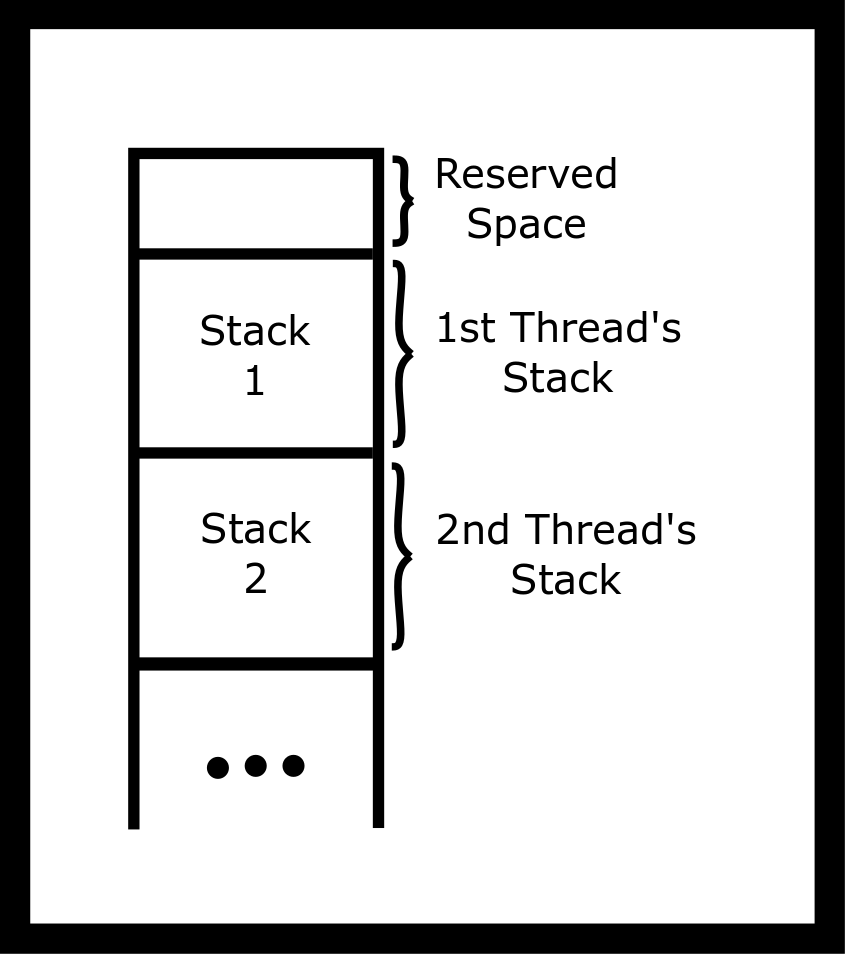
\includegraphics{threads/images/thread_stack.png}
\caption{Thread address space}
\end{figure}

\subsection{How many threads can my process have?}\label{how-many-threads-can-my-process-have}

You can have more than one thread running inside a process. You get the first thread for free! It runs the code you write inside `main'. If you need more threads you can call \keyword{pthread\_create} to create a new thread using the pthread library. You'll need to pass a pointer to a function so that the thread knows where to start.

The threads you create all live inside the same virtual memory because they are part of the same process. Thus they can all see the heap, the global variables and the program code etc. Thus you can have two (or more) CPUs working on your program at the same time and inside the same process. It's up to the operating system to assign the threads to CPUs. If you have more active threads than CPUs then the kernel will assign the thread to a CPU for a short duration (or until it runs out of things to do) and then will automatically switch the CPU to work on another thread. For example, one CPU might be processing the game AI while another thread is computing the graphics output.

\section{Simple Usage}\label{simple-usage}

To use pthreads you will need to include \keyword{pthread.h} and compile with \keyword{-pthread} (or \keyword{-lpthread}) compiler option. This option tells the compiler that your program requires threading support. To create a thread use the function \keyword{pthread\_create}. This function takes four arguments:

\begin{code}[language=C]
int pthread_create(pthread_t *thread, const pthread_attr_t *attr,
                   void *(*start_routine) (void *), void *arg);
\end{code}

\begin{itemize}
\tightlist
\item
  The first is a pointer to a variable that will hold the id of the newly created thread.
\item
  The second is a pointer to attributes that we can use to tweak and tune some of the advanced features of pthreads.
\item
  The third is a pointer to a function that we want to run
\item
  Fourth is a pointer that will be given to our function
\end{itemize}

The argument \keyword{void *(*start\_routine) (void *)} is difficult to read! It means a pointer that takes a \keyword{void *} pointer and returns a \keyword{void *} pointer. It looks like a function declaration except that the name of the function is wrapped with \keyword{(* .... )}

\begin{code}[language=C]
#include <stdio.h>
#include <pthread.h>
// remember to set compilation option -pthread

void *busy(void *ptr) {
// ptr will point to "Hi"
    puts("Hello World");
    return NULL;
}
int main() {
    pthread_t id;
    pthread_create(&id, NULL, busy, "Hi");
#if loop_forever // Loop forever
    while (1) {}
#else // Join Threads
    void *result;
    pthread_join(id, &result);
#endif
}
\end{code}

In the above example, \keyword{result} will be \keyword{null} because the busy function returned \keyword{null}. We need to pass the address-of result because \keyword{pthread\_join} will be writing into the contents of our pointer.

\section{Pthread Functions}\label{more-pthread-functions}

\begin{itemize}
\item \keyword{pthread\_create}. Creates a new thread. Every thread that gets created gets a new stack. For example if you call \keyword{pthread\_create} twice, Your process will contain three stacks - one for each thread. The first thread is created when the process starts, and you created two more. Actually there can be more stacks than this, but let's keep it simple. The important idea is that each thread requires a stack because the stack contains automatic variables and the old CPU PC register, so that it can back to executing the calling function after the function is finished.
\item \keyword{pthread\_cancel} stops a thread. Note the thread may not actually be stopped immediately. For example it can be terminated when the thread makes an operating system call (e.g. \keyword{write}). In practice, \keyword{pthread\_cancel} is rarely used because it does not give a thread an opportunity to clean up after itself (for example, it may have opened some files). An alternative implementation is to use a boolean (int) variable whose value is used to inform other threads that they should finish and clean up.
\item \keyword{pthread\_exit(void *)} stops the calling thread i.e.~the thread never returns after calling \keyword{pthread\_exit}. The pthread library will automatically finish the process if there are no other threads running. \keyword{pthread\_exit(...)} is equivalent to returning from the thread's function; both finish the thread and also set the return value (void *pointer) for the thread. Calling \keyword{pthread\_exit} in the the \keyword{main} thread is a common way for simple programs to ensure that all threads finish. For example, in the following program, the \keyword{myfunc} threads will probably not have time to get started. On the other hand \keyword{exit()} exits the entire process and sets the processes exit value. This is equivalent to \keyword{return ();} in the main method. All threads inside the process are stopped. Note the \keyword{pthread\_exit} version creates thread zombies, however this is not a long-running processes, so we don't care. 

\begin{code}[language=C]
int main() {
  pthread_t tid1, tid2;
  pthread_create(&tid1, NULL, myfunc, "Jabberwocky");
  pthread_create(&tid2, NULL, myfunc, "Vorpel");
  if (keep_threads_going) {
    pthread_exit(NULL); 
  } else {
    exit(42); //or return 42;
  }

  // No code is run after exit
}
\end{code}

\item \keyword{pthread\_join()} waits for a thread to finish and records its return value. Finished threads will continue to consume resources. Eventually, if enough threads are created, \keyword{pthread\_create} will fail. In practice, this is only an issue for long-running processes but is not an issue for simple, short-lived processes as all thread resources are automatically freed when the process exits. This is equivalent to turning your children into zombies, so keep this in mind for long running processes. In the exit example, we could also wait on all the threads.

\begin{code}[language=C]
// ...
  void* result;
  pthread_join(tid1, &result);
  pthread_join(tid2, &result); 
  return 42;
// ...
\end{code}

\item You've heard about this already, but how can a thread be terminated? 
\begin{itemize}
  \tightlist
\item Returning from the thread function 
\item Calling \keyword{pthread\_exit} 
\item Cancelling the thread with \keyword{pthread\_cancel} 
\item Terminating the process (e.g.~SIGTERM); exit(); returning from \keyword{main}
\end{itemize}

\end{itemize}

\section{Race Conditions}

Race conditions are whenever the outcome of a program is determined by its sequence of events. Meaning that the same program can run multiple times and depending on how the kernel schedules the threads could produce inaccurate results. Take for example this race condition with one thread. We create a stack variable and pass it to our pthread function.

\begin{code}
pthread_t start_threads() {
  int start = 42;
  pthread_t tid;
  pthread_create(&tid, 0, myfunc, &start); // ERROR!
  return tid;
}
\end{code}

The above code is invalid because the function \keyword{start\_threads} will likely return before \keyword{myfunc} even starts. The function passes the address-of \keyword{start}, however by the time \keyword{myfunc} is executes, \keyword{start} is no longer in scope and its address will re-used for another variable. This ia race condition because there is a situation where the thread that called pthread\_create could be suspended indefinitely, and the code actually works. One way we can fix this is keep the function from returning before the thread finishes.

\begin{code}
void start_threads() {
  int start = 42;
  void *result;
  pthread_t tid;
  pthread_create(&tid, 0, myfunc, &start); // OK - start will be valid!
  pthread_join(tid, &result);
}
\end{code}

Here is another small race condition. The following code is supposed to start ten threads with values 0,1,2,3,\ldots{}9 However, when run prints out \keyword{1 7 8 8 8 8 8 8 8 10}! Can you see why?

\begin{code}[language=C]
#include <pthread.h>
void* myfunc(void* ptr) {
    int i = *((int *) ptr);
    printf("%d ", i);
    return NULL;
}

int main() {
    // Each thread gets a different value of i to process
    int i;
    pthread_t tid;
    for(i =0; i < 10; i++) {
        pthread_create(&tid, NULL, myfunc, &i); // ERROR
    }
    pthread_exit(NULL);
}
\end{code}

The above code suffers from a \keyword{race condition} - the value of i is changing. The new threads start later (in the example output the last thread starts after the loop has finished). To overcome this race-condition, we will give each thread a pointer to it's own data area. For example, for each thread we may want to store the id, a starting value and an output value. We will instead treat i as a pointer and cast it by value.

\begin{code}[language=C]
void* myfunc(void* ptr) {
    int data = ((int) ptr);
    printf("%d ", data);
    return NULL;
}

int main() {
    // Each thread gets a different value of i to process
    int i;
    pthread_t tid;
    for(i =0; i < 10; i++) {
        pthread_create(&tid, NULL, myfunc, (void *)i);
    }
    pthread_exit(NULL);
}
\end{code}

Some functions e.g. asctime, getenv, strtok, strerror not thread-safe. Let's look at a simple function that is also not `thread-safe' The result buffer could be stored in global memory. This is good - we wouldn't want to return a pointer to an invalid address on the stack, but there's only one result buffer in the entire memory. If two threads were to use it at the same time then one would corrupt the other:

\begin{code}[language=C]
char *to_message(int num) {
    char static result [256];
    if (num < 10) sprintf(result, "%d : blah blah" , num);
    else strcpy(result, "Unknown");
    return result;
}
\end{code}

There are ways around this like using synchronization locks. These are synchronization locks that are used to prevent race conditions and ensure proper synchronization between threads running in the same program. In addition, these locks are conceptually identical to the primitives used inside the kernel.

In case you were wondering, you can fork inside a process with multiple threads! However, the child process only has a single thread, which is a clone of the thread that called \keyword{fork}. We can see this as a simple example, where the background threads never print out a second message in the child process.

\begin{code}[language=C]
#include <pthread.h>
#include <stdio.h>
#include <unistd.h>

static pid_t child = -2;

void *sleepnprint(void *arg) {
  printf("%d:%s starting up...\n", getpid(), (char *) arg);

  while (child == -2) {sleep(1);} /* Later we will use condition variables */

  printf("%d:%s finishing...\n",getpid(), (char*)arg);

  return NULL;  
}
int main() {
  pthread_t tid1, tid2;
  pthread_create(&tid1,NULL, sleepnprint, "New Thread One");
  pthread_create(&tid2,NULL, sleepnprint, "New Thread Two");
  
  child = fork();
  printf("%d:%s\n",getpid(), "fork()ing complete");
  sleep(3);
    
  printf("%d:%s\n",getpid(), "Main thread finished");
  
  pthread_exit(NULL);
  return 0; /* Never executes */
}
\end{code}

\begin{verbatim}
8970:New Thread One starting up...
8970:fork()ing complete
8973:fork()ing complete
8970:New Thread Two starting up...
8970:New Thread Two finishing...
8970:New Thread One finishing...
8970:Main thread finished
8973:Main thread finished
\end{verbatim}

In practice, creating threads before forking can lead to unexpected errors because (as demonstrated above) the other threads are immediately terminated when forking. Another thread might have just lock a mutex (e.g.~by calling malloc) and never unlock it again. Advanced users may find \keyword{pthread\_atfork} useful however we suggest you usually try to avoid creating threads before forking unless you fully understand the limitations and difficulties of this approach.

\subsection{How can I find out more?}\label{how-can-i-find-out-more}

\begin{itemize}
\item \href{http://man7.org/linux/man-pages/man3/pthread_create.3.html}{man page} 
\item \href{http://man7.org/linux/man-pages/man7/pthreads.7.html}{pthread reference guide} 
\item \href{http://www.thegeekstuff.com/2012/04/terminate-c-thread/}{Concise third party sample code explaining create, join and exit}
\end{itemize}


\begin{aside}

\subsection{Embarrassingly Parallel Problems}\label{embarrassingly-parallel-problems}

The study of parallel algorithms has exploded over the past few years. An embarrassingly parallel problem is any problem that needs little effort to turn parallel. A lot of them have some synchronization concepts with them but not always. You already know a parallelizable algorithm, Merge Sort!

\begin{code}[language=C]
void merge_sort(int *arr, size_t len){
   if(len > 1){
   //Mergesort the left half
   //Mergesort the right half
   //Merge the two halves
   }
\end{code}

With your new understanding of threads, all you need to do is create a thread for the left half, and one for the right half. Given that your CPU has multiple real cores, you will see a speedup in accordance with \href{https://en.wikipedia.org/wiki/Amdahl's_law}{Amdahl's Law}. The time complexity analysis gets interesting here as well. The parallel algorithm runs in $O(\log^3(n))$ running time (because we fancy analysis assuming that we have a lot of cores.

In practice though, we typically do two changes. One, once the array gets small enough, we ditch the parallel mergesort algorithm and do a quicksort or other algorithm that works fast on small arrays (something something cache coherency). The other thing that we know is that CPUs don't have infinite cores. To get around that, we typically keep a worker pool. You won't see the speedup right away because of things like cache coherency and scheduling extra threads.

\subsection{Another problem, Parallel Map}\label{another-problem-parallel-map}

Say we want to apply a function to an entire array, one element at a time.

\begin{code}[language=C]

int *map(int (*func)(int), int *arr, size_t len){
  int *ret = malloc(len*sizeof(*arr));
  for(size_t i = 0; i < len; ++i) 
      ret[i] = func(arr[i]);
  return ret;
}
\end{code}

Since none of the elements depend on any other element, how would you go about parallelizing this? What do you think would be the best way to split up the work between threads.

\subsection{Scheduling}\label{scheduling}

There are a few ways to split up the work. 

\begin{itemize}
\item \keyword{static scheduling} break up the problems into fixed size chunks (predetermined) and have each thread work on each of the chunks. This works well when each of the subproblems take roughly the same time because there is no additional overhead. All you need to do is write a loop and give the map function to each subarray. 
\item \keyword{dynamic scheduling} as a new problem becomes available have a thread serve it. This is useful when you don't know how long the scheduling will take 
\item \keyword{guided scheduling} This is a mix of the above with a mix of the benefits and the tradeoffs. You start with a static scheduling and move slowly to dynamic if needed 
\item \keyword{runtime scheduling} You have absolutely no idea how long the problems are going to take. Instead of deciding it yourself, let the program decide what to do!
\end{itemize}

\href{https://software.intel.com/en-us/articles/openmp-loop-scheduling}{source}, but no need to memorize.


\subsection{Other Problems}\label{other-problems}

From \href{https://en.wikipedia.org/wiki/Embarrassingly_parallel}{Wikipedia} 
\begin{itemize}
\tightlist
\item Serving static files on a webserver to multiple users at once. 
\item The Mandelbrot set, Perlin noise and similar images, where each point is calculated independently. 
\item Rendering of computer graphics. In computer animation, each frame may be rendered independently (see parallel rendering). 
\item Brute-force searches in cryptography.
\item Notable real-world examples include distributed.net and proof-of-work systems used in cryptocurrency. 
\item BLAST searches in bioinformatics for multiple queries (but not for individual large queries) 
\item Large scale facial recognition systems that compare thousands of arbitrary acquired faces (e.g., a security or surveillance video via closed-circuit television) with similarly large number of previously stored faces (e.g., a rogues gallery or similar watch list).
\item Computer simulations comparing many independent scenarios, such as climate models. 
\item Evolutionary computation metaheuristics such as genetic algorithms. 
\item Ensemble calculations of numerical weather prediction. 
\item Event simulation and reconstruction in particle physics. 
\item The marching squares algorithm 
\item Sieving step of the quadratic sieve and the number field sieve. 
\item Tree growth step of the random forest machine learning technique. 
\item Discrete Fourier Transform where each harmonic is independently calculated.
\end{itemize}

\end{aside}

\section{Topics}\label{topics}

\begin{itemize}
\tightlist
\item
pthread lifecycle
\item
Each thread has a stack
\item
Capturing return values from a thread
\item
Using \keyword{pthread\_join}
\item
Using \keyword{pthread\_create}
\item
Using \keyword{pthread\_exit}
\item
Under what conditions will a process exit
\end{itemize}

\section{Questions}\label{questions}

\begin{itemize}
\tightlist
\item
What happens when a pthread gets created? (you don't need to go into super specifics)
\item
Where is each thread's stack?
\item
How do you get a return value given a \keyword{pthread\_t}? What are the ways a thread can set that return value? What happens if you discard the return value?
\item
Why is \keyword{pthread\_join} important (think stack space, registers, return values)?
\item
What does \keyword{pthread\_exit} do under normal circumstances (ie you are not the last thread)? What other functions are called when you call pthread\_exit?
\item
Give me three conditions under which a multithreaded process will exit. Can you think of any more?
\item
What is an embarrassingly parallel problem?
\end{itemize}

\bibliographystyle{plainnat}
\bibliography{threads/threads}

%\chapter{Synchronization}

\epigraph{When multithreading gets interesting}{Bhuvy}

Synchronization are a series of mechanisms to control what threads are allowed to perform what operation at a time.
Most of the time, the threads can progress without having to communicate, but every so often two or more threads may want to access a critical section.
A critical section is a section of code that can only be executed by one thread at a time, if the program is to function correctly.
If two threads (or processes) were to execute code inside the critical section at the same time, it is possible that program may no longer have correct behavior.

As we said in the previous chapter, race conditions happen when an operation touches a piece of memory at the same time as another thread.
If the memory location is only accessible by one thread, for example the automatic variable \keyword{i} below, then there is no possibility of a race condition and no Critical Section associated with \keyword{i}.
However the \keyword{sum} variable is a global variable and accessed by two threads.
It is possible that two threads may attempt to increment the variable at the same time.

\begin{lstlisting}[language=C]
#include <stdio.h>
#include <pthread.h>

int sum = 0; //shared

void *countgold(void *param) {
    int i; //local to each thread
    for (i = 0; i < 10000000; i++) {
        sum += 1;
    }
    return NULL;
}

int main() {
    pthread_t tid1, tid2;
    pthread_create(&tid1, NULL, countgold, NULL);
    pthread_create(&tid2, NULL, countgold, NULL);

    //Wait for both threads to finish:
    pthread_join(tid1, NULL);
    pthread_join(tid2, NULL);

    printf("ARRRRG sum is %d\n", sum);
    return 0;
}
\end{lstlisting}

Typical output of the above code is \keyword{ARGGGH sum is <some number less than expected>} because there is a race condition.
The code does not stop two threads from reading-writing \keyword{sum} at the same time.
For example, both threads copy the current value of sum into CPU that runs each thread (let's pick 123).
Both threads increment one to their own copy.
Both threads write back the value (124).
If the threads had accessed the sum at different times then the count would have been 125.
A few of the possible different orderings are below.

Permissible Pattern

\begin{tabular}{ l | r }
  Thread 1 & Thread 2 \\ \hline
  Load Addr, Add 1 (i=1 locally) & ...  \\
  Store (i=1 globally) & ...  \\
  ... & Load Addr, Add 1 (i=2 locally)  \\
  ... & Store (i=2 globally)  \\
\end{tabular}

Partial Overlap

\begin{tabular}{ l | r }
Thread 1 & Thread 2 \\ \hline
Load Addr, Add 1 (i=1 locally) & ... \\
Store (i=1 globally) & Load Addr, Add 1 (i=1 locally) \\
... & Store (i=1 globally) \\
\end{tabular}

Full Overlap
\begin{tabular}{ l | r }
Thread 1 & Thread 2 \\ \hline
Load Addr, Add 1 (i=1 locally) & Load Addr, Add 1 (i=1 locally) \\
Store (i=1 globally) & Store (i=1 globally) \\
\end{tabular}

We would like the first pattern of the code being mutually exclusive.
Which leads us to our first synchronization primitive, a Mutex.

\section{Mutex}

To ensure only one thread at a time can access a global variable, use a mutex -- short for Mutual Exclusion.
If one thread is currently inside a critical section we would like another thread to wait until the first thread is complete.
A mutex isn't a primitive in the truest sense, though it is one of the smallest pieces of data structures that has some threading API sense.
A mutex also isn't really a data structure.
It is an abstract data type, much like you learned in your data structures class.
There are many ways to implement a mutex, and we'll give a few in this chapter.
For right now let's use the black box that the pthread library gives us.
Here is how we declare a mutex.

\begin{lstlisting}[language=C]
pthread_mutex_t m = PTHREAD_MUTEX_INITIALIZER; // global variable
pthread_mutex_lock(&m); // start of Critical Section
// Critical section
pthread_mutex_unlock(&m); //end of Critical Section
\end{lstlisting}

\subsection{Mutex Lifetime}

There are a few ways of initializing a mutex.
You can use the macro \keyword{PTHREAD\_MUTEX\_INITIALIZER} only for global (`static') variables.
\keyword{m = PTHREAD\_MUTEX\_INITIALIZER} is exactly equivalent to the more general purpose \keyword{pthread\_mutex\_init(&m,NULL)} but for our purposes it is the same.
The init version includes options to trade performance for additional error-checking and advanced sharing options.
The init version also makes sure that the mutex is correctly initialized after the call, global mutexes are initialized on first lock.
You can also call the init function inside of a program for a mutex located on the heap.

\begin{lstlisting}[language=C]
pthread_mutex_t *lock = malloc(sizeof(pthread_mutex_t));
pthread_mutex_init(lock, NULL);
//later
pthread_mutex_destroy(lock);
free(lock);
\end{lstlisting}

Once we are finished with the mutex we should also call \keyword{pthread\_mutex\_destroy(&m)} too.
Note, you can only destroy an unlocked mutex, destroy on a locked mutex is undefined behavior.
Things to keep in mind about \keyword{init} and \keyword{destroy}
You don't need to destroy a mutex created with the global initializer.

\begin{enumerate}
\item Multiple threads init/destroy has undefined behavior
\item Destroying a locked mutex has undefined behavior
\item Keep to the pattern of one and only one thread initializing a mutex.
\item Copying the bytes of the mutex to a new memory location and then using the copy is \emph{not} supported.
  To reference a mutex, you have to have a pointer to that memory address.
\end{enumerate}

\subsection{Mutex Usages}

How would I use a mutex?
Here is a complete example in the spirit of the earlier piece.

\begin{lstlisting}[language=C]
#include <stdio.h>
#include <pthread.h>

// Create a mutex this ready to be locked!
pthread_mutex_t m = PTHREAD_MUTEX_INITIALIZER;

int sum = 0;

void *countgold(void *param) {
    int i;

    //Same thread that locks the mutex must unlock it
    //Critical section is just 'sum += 1'
    //However locking and unlocking a million times
    //has significant overhead

    pthread_mutex_lock(&m);

    // Other threads that call lock will have to wait until we call unlock

    for (i = 0; i < 10000000; i++) {
        sum += 1;
    }
    pthread_mutex_unlock(&m);
    return NULL;
}

int main() {
    pthread_t tid1, tid2;
    pthread_create(&tid1, NULL, countgold, NULL);
    pthread_create(&tid2, NULL, countgold, NULL);

    pthread_join(tid1, NULL);
    pthread_join(tid2, NULL);

    printf("ARRRRG sum is %d\n", sum);
    return 0;
}
\end{lstlisting}

In the code above, the thread gets the lock to the counting house before entering.
The critical section is only the \keyword{sum+=1} so the following version is also correct.

\begin{lstlisting}[language=C]
    for (i = 0; i < 10000000; i++) {
        pthread_mutex_lock(&m);
        sum += 1;
        pthread_mutex_unlock(&m);
    }
    return NULL;
}
\end{lstlisting}

This process runs slower because we lock and unlock the mutex a million times, which is expensive - at least compared with incrementing a variable.
In this simple example, we didn't really need threads - we could have added up twice!
A faster multi-thread example would be to add one million using an automatic (local) variable and only then adding it to a shared total after the calculation loop has finished:

\begin{lstlisting}[language=C]
    int local = 0;
    for (i = 0; i < 10000000; i++) {
       local += 1;
    }

    pthread_mutex_lock(&m);
    sum += local;
    pthread_mutex_unlock(&m);

    return NULL;
}
\end{lstlisting}

Obviously if you know the Gaussian sum, you can avoid race conditions altogether, but this is just for illustration.

Starting with the gotchas.
Firstly, C Mutexes do not lock variables.
A mutex is not that smart.
It works with code, not data.
If I lock a mutex, the other threads will continue.
It's only when a thread attempts to lock a mutex that is already locked, will the thread have to wait.
As soon as the original thread unlocks the mutex, the second (waiting) thread will acquire the lock and be able to continue.
The following code creates a mutex that does effectively nothing.

\begin{lstlisting}[language=C]
int a;
pthread_mutex_t m1 = PTHREAD_MUTEX_INITIALIZER,
                 m2 = = PTHREAD_MUTEX_INITIALIZER;
// later
// Thread 1
pthread_mutex_lock(&m1);
a++;
pthread_mutex_unlock(&m1);

// Thread 2
pthread_mutex_lock(&m2);
a++;
pthread_mutex_unlock(&m2);
\end{lstlisting}

Here are some other gotchas in no particular order
\begin{enumerate}
\item Don't cross the streams!
If you are using threads, don't fork in the middle of your program.
This means any time after your mutexes have been initialized.
\item The thread that locks a mutex is the only thread that can unlock it.
\item Each program can have multiple mutex locks.
  You can design your program to have one lock per data structure,
  one lock per heap,
  or one lock per set of data structures
  If you only have one lock, then they may be significant contention for the lock between two threads that was unnecessary.
  For example if two threads were updating two different counters, it might not be necessary to use the same lock.
\item Locks are only tools.
  They don't spot critical sections for you!
\item There will always be a small amount of overhead of calling \keyword{pthread\_mutex\_lock} and \keyword{pthread\_mutex\_unlock}.
However, this is the price you pay for correctly functioning programs!
\item
  Not unlocking a mutex due to an early return during an error condition
\item
  Resource leak (not calling \keyword{pthread\_mutex\_destroy})
\item
  Using an uninitialized mutex or using a mutex that has already been destroyed
\item
  Locking a mutex twice on a thread without unlocking first
\item
  Deadlock
\end{enumerate}

\subsection{Mutex Implementation}

So we have this cool data structure.
How do we implement it?
First a naive, incorrect implementation is shown below.
The \keyword{unlock} function simply unlocks the mutex and returns.
The lock function first checks to see if the lock is already locked.
If it is currently locked, it will keep checking again until another thread has unlocked the mutex.

\begin{lstlisting}[language=C]
// Version 1 (Incorrect!)

void lock(mutex_t *m) {
  while(m->locked) { /*Locked? Never-mind - just loop and check again!*/ }

  m->locked = 1;
}

void unlock(mutex_t *m) {
  m->locked = 0;
}
\end{lstlisting}

Version 1 uses `busy-waiting' unnecessarily wasting CPU resources.
However, there is a more serious problem.
We have a race-condition!
If two threads both called \keyword{lock} concurrently, it is possible that both threads would read \keyword{m\_locked} as zero.
Thus both threads would believe they have exclusive access to the lock and both threads will continue.

We might attempt to reduce the CPU overhead a little by calling \keyword{pthread\_yield()} inside the loop - pthread\_yield suggests to the operating system that the thread does not use the CPU for a short while, so the CPU may be assigned to threads that are waiting to run.
But does not fix the race-condition.
We need a better implementation.

\subsection{Extra: Implementing a Mutex with hardware}

We can use C11 Atomics to do that perfectly!
A complete solution is detailed here.
This is a spinlock mutex, \href{https://locklessinc.com/articles/mutex_cv_futex/}{futex} implementations can be found online.

First the data structure and initialization code.

\begin{lstlisting}[language=C]
typedef struct mutex_{
    // We need some variable to see if the lock is locked
    atomic_int_least8_t lock;
    // A mutex needs to keep track of its owner so
    // Another thread can't unlock it
    pthread_t owner;
} mutex;

#define UNLOCKED 0
#define LOCKED 1
#define UNASSIGNED_OWNER 0

int mutex_init(mutex* mtx){
    // Some simple error checking
    if(!mtx){
        return 0;
    }
    // Not thread safe the user has to take care of this
    atomic_init(&mtx->lock, UNLOCKED);
    mtx->owner = UNASSIGNED_OWNER;
    return 1;
}
\end{lstlisting}

This is the initialization code, nothing fancy here.
We set the state of the mutex to unlocked and set the owner to locked.

\begin{lstlisting}[language=C]
int mutex_lock(mutex* mtx){
    int_least8_t zero = UNLOCKED;
    while(!atomic_compare_exchange_weak_explicit
            (&mtx->lock,
             &zero,
             LOCKED,
             memory_order_seq_cst,
             memory_order_seq_cst)){
        zero = UNLOCKED;
        sched_yield(); // Use system calls for scheduling speed
    }
    // We have the lock now
    mtx->owner = pthread_self();
    return 1;
}
\end{lstlisting}

What does this code do?
Well to start it it initializes a variable that we will keep as the unlocked state.
\href{https://en.wikipedia.org/wiki/Compare-and-swap}{Atomic Compare and Exchange} is an instruction supported by most modern architectures (on x86 it's \keyword{lock cmpxchg}).
The pseudocode for this operation looks like this

\begin{lstlisting}[language=C]
int atomic_compare_exchange_pseudo(int* addr1, int* addr2, int val){
    if(*addr1 == *addr2){
        *addr1 = val;
        return 1;
    }else{
        *addr2 = *addr1;
        return 0;
    }
}
\end{lstlisting}

Except it is all done \emph{atomically} meaning in one uninterruptible operation.
What does the \emph{weak} part mean?
Well atomic instructions are prone to \textbf{spurious failures} meaning that there are two versions to these atomic functions a \emph{strong} and a \emph{weak} part, strong guarantees the success or failure while weak may fail even when the operation succeeds.
These are the same spurious failures that you'll see in condition variables below.
We are using weak because weak is faster, and we are in a loop!
That means we are okay if it fails a little bit more often because we will just keep spinning around anyway.

Inside the while loop, we have failed to grab the lock!
We reset zero to unlocked and sleep for a little while.
When we wake up we try to grab the lock again.
Once we successfully swap, we are in the critical section!
We set the mutex's owner to the current thread for the unlock method and return successful.

How does this guarantee mutual exclusion, when working with atomics we are not entirely sure!
But in this simple example, we can because the thread that is able to successfully expect the lock to be UNLOCKED (0) and swap it to a LOCKED (1) state is considered the winner.
How do we implement unlock?

\begin{lstlisting}[language=C]
int mutex_unlock(mutex* mtx){
    if(unlikely(pthread_self() != mtx->owner)){
        return 0; //You can't unlock a mutex if you aren't the owner
    }
    int_least8_t one = 1;
    //Critical section ends after this atomic
    mtx->owner = UNASSIGNED_OWNER;
    if(!atomic_compare_exchange_strong_explicit(
                &mtx->lock,
                &one,
                UNLOCKED,
                memory_order_seq_cst,
                memory_order_seq_cst)){
        //The mutex was never locked in the first place
        return 0;
    }
    return 1;
}
\end{lstlisting}

To satisfy the api, you can't unlock the mutex unless you are the one who owns it.
Then we unassign the mutex owner, because critical section is over after the atomic.
We want a strong exchange because we don't want to block (pthread\_mutex\_unlock doesn't block).
We expect the mutex to be locked, and we swap it to unlock.
If the swap was successful, we unlocked the mutex.
If the swap wasn't, that means that the mutex was UNLOCKED and we tried to switch it from UNLOCKED to UNLOCKED, preserving the non blocking of unlock.

What is this memory order business?
We were talking about memory fences earlier, here it is!
We won't go into detail because it is outside the scope of this course but not the scope of \href{https://gcc.gnu.org/wiki/Atomic/GCCMM/AtomicSync}{this article}.
Basically we need consistency to make sure no loads or stores are ordered before or after.
You need to create dependency chains for more efficient ordering.

\subsection{Semaphore}

A semaphore is another synchronization primitive.
It is initialized to some value.
Threads can either \keyword{sem\_wait} or \keyword{sem\_post} which lowers or increases the value.
If the value reaches zero and a wait is called, the thread will be blocked until a post is called.

Using a semaphore is as easy as creating a mutex.
First decide if the initial value should be zero or some other value, for example the number of remaining spaces in an array.
Unlike pthread mutex there are not shortcuts to creating a semaphore - use \keyword{sem\_init}.

\begin{lstlisting}[language=C]
#include <semaphore.h>

sem_t s;
int main() {
  sem_init(&s, 0, 10); // returns -1 (=FAILED) on OS X
  sem_wait(&s); // Could do this 10 times without blocking
  sem_post(&s); // Announce that we've finished (and one more resource item is available; increment count)
  sem_destroy(&s); // release resources of the semaphore
}
\end{lstlisting}

When using a semaphore, wait and post can be called from different threads!
Unlike a mutex, the increment and decrement can be from different threads.


This becomes especially useful if you want to use a semaphore to implement a mutex.
A mutex is a semaphore that always \keyword{waits} before it \keyword{posts}.
Some textbooks will refer to a mutex as a binary semaphore.
You do have to be careful to never add more than one to a semaphore or otherwise your mutex abstraction breaks.
That is usually why a mutex is used to implement a semaphore and vice versa.

\begin{itemize}
\item Initialize the semaphore with a count of one.
\item Replace \keyword{pthread\_mutex\_lock} with \keyword{sem\_wait}
\item Replace \keyword{pthread\_mutex\_unlock} with \keyword{sem\_post}
\end{itemize}

\begin{lstlisting}[language=C]
sem_t s;
sem_init(&s, 0, 1);

sem_wait(&s);
// Critical Section
sem_post(&s);
\end{lstlisting}

But be warned, it isn't the same!
A mutex can handle what we call lock inversion well.
Meaning the following code breaks with a traditional mutex, but produces a race condition with threads.

\begin{lstlisting}[language=C]
// Thread 1
sem_wait(&s);
// Critical Section
sem_post(&s);

// Thread 2
// Some threads just want to see the world burn
sem_post(&s);

// Thread 3
sem_wait(&s);
// Not thread safe!
sem_post(&s);
\end{lstlisting}

If we replace it with mutex lock it won't work now.

\begin{lstlisting}[language=C]
// Thread 1
mutex_lock(&s);
// Critical Section
mutex_unlock(&s);

// Thread 2
// Foiled!
mutex_unlock(&s);

// Thread 3
mutex_lock(&s);
// Now it's thread safe
mutex_unlock(&s);
\end{lstlisting}

\subsubsection{Signal Safety}

Also, keyword{sem\_post} is one of a handful of functions that can be correctly used inside a signal handler \keyword{pthread\_mutex\_unlock} is not.
This means we can release a waiting thread which can now make all of the calls that we were not allowed to call inside the signal handler itself e.g. \keyword{printf}.
Here is some code that utilizes this;

\begin{lstlisting}[language=C]
#include <stdio.h>
#include <pthread.h>
#include <signal.h>
#include <semaphore.h>
#include <unistd.h>

sem_t s;

void handler(int signal) {
    sem_post(&s); /* Release the Kraken! */
}

void *singsong(void *param) {
    sem_wait(&s);
    printf("I had to wait until your signal released me!\n");
}

int main() {
    int ok = sem_init(&s, 0, 0 /* Initial value of zero*/);
    if (ok == -1) {
       perror("Could not create unnamed semaphore");
       return 1;
    }
    signal(SIGINT, handler); // Too simple! See Signals chapter

    pthread_t tid;
    pthread_create(&tid, NULL, singsong, NULL);
    pthread_exit(NULL); /* Process will exit when there are no more threads */
}
\end{lstlisting}

Other uses for semaphores are keeping track of empty spaces in arrays. We will discuss these in the thread-safe data structures section.

\section{Condition Variables}

Condition variables allow a set of threads to sleep until woken up.
You can wake up one thread or all threads that are sleeping.
If you only wake one thread then the operating system will decide which thread to wake up.
You don't wake threads directly instead you `signal' the condition variable, which then will wake up one (or all) threads that are sleeping inside the condition variable.

Condition variables are also used with a mutex and with a loop, so when woken up they have to check a condition in a critical section.
If you just need to be woken up not in a critical section, there are other ways to do this in POSIX.
Threads sleeping inside a condition variable are woken up by calling \keyword{pthread\_cond\_broadcast} (wake up all) or \keyword{pthread\_cond\_signal} (wake up one).
Note despite the function name, this has nothing to do with POSIX \keyword{signal}s!

Occasionally a waiting thread may appear to wake up for no reason. This is called a \emph{spurious wake}.
If you read the hardware implementation of a mutex section, this is similar.
This is not an issue because you always use \keyword{wait} inside a loop that tests a condition that must be true to continue.

Why do spurious wakeups happen? For performance.
On multi-CPU systems, it is possible that a race-condition could cause a wake-up (signal) request to be unnoticed.
The kernel may not detect this lost wake-up call but can detect when it might occur.
To avoid the potential lost signal, the thread is woken up so that the program code can test the condition again.

\begin{comment}

\subsection{Extra: Why do Condition Variables also need a mutex?}

Condition variables need a mutex for three reasons. The simplest to understand is that it prevents an early wakeup message (\keyword{signal} or \keyword{broadcast} functions) from being `lost.' Imagine the following sequence of events (time runs down the page) where the condition is satisfied \emph{just before} \keyword{pthread\_cond\_wait} is called. In this example the wake-up signal is lost!

Thread 1 \textbar{} Thread 2 -------------------------\textbar{}--------- \keyword{while( answer < 42) {} \textbar{} \textbar{} \keyword{answer++} \textbar{} \keyword{p\_cond\_signal(cv)} \keyword{p\_cond\_wait(cv,m)} \textbar{}

If both threads had locked a mutex, the signal can not be sent until \emph{after} \keyword{pthread\_cond\_wait(cv, m)} is called (which then internally unlocks the mutex)

A second common reason is that updating the program state (\keyword{answer} variable) typically requires mutual exclusion - for example multiple threads may be updating the value of \keyword{answer}.

A third and subtle reason is to satisfy real-time scheduling concerns which we only outline here: In a time-critical application, the waiting thread with the \emph{highest priority} should be allowed to continue first. To satisfy this requirement the mutex must also be locked before calling \keyword{pthread\_cond\_signal} or \keyword{pthread\_cond\_broadcast} . For the curious, a longer and historical discussion is \href{https://groups.google.com/forum/?hl=ky\#!msg/comp.programming.threads/wEUgPq541v8/ZByyyS8acqMJ}{here}.

\end{comment}

\subsection{Condition wait Wait Example}

The call \keyword{pthread\_cond\_wait} performs three actions:

\begin{enumerate}
\item Unlock the mutex; it must be locked.
\item Sleeps until \keyword{pthread\_cond\_signal} is called on the same condition variable)
\item Before returning, locks the mutex
\end{enumerate}

Condition variables are \emph{always} used with a mutex lock.
Before calling \emph{wait}, the mutex lock must be locked and \emph{wait} must be wrapped with a loop.

\begin{lstlisting}[language=C]
pthread_cond_t cv;
pthread_mutex_t m;
int count;

// Initialize
pthread_cond_init(&cv, NULL);
pthread_mutex_init(&m, NULL);
count = 0;

// Thread 1
pthread_mutex_lock(&m);
while (count < 10) {
   pthread_cond_wait(&cv, &m);
  /* Remember that cond_wait unlocks the mutex before blocking (waiting)! */
  /* After unlocking, other threads can claim the mutex. */
  /* When this thread is later woken it will */
  /* re-lock the mutex before returning */
}
pthread_mutex_unlock(&m);

//later clean up with pthread_cond_destroy(&cv); and mutex_destroy


// Thread 2:
while (1) {
  pthread_mutex_lock(&m);
  count++;
  pthread_cond_signal(&cv);
  /* Even though the other thread is woken up it cannot not return */
  /* from pthread_cond_wait until we have unlocked the mutex. This is */
  /* a good thing! In fact, it is usually the best practice to call */
  /* cond_signal or cond_broadcast before unlocking the mutex */
  pthread_mutex_unlock(&m);
}
\end{lstlisting}

This is a pretty naive example, but it shows that we can tell threads to wake up in a standardized manner. In the next section, we will use these to implement efficient blocking data structures.

\section{Thread Safe Data Structures}

Naturally, we want our data structures to be thread safe as well!
We can use mutexes and synchronization primitives to make that happen.
First a few definitions.
Atomicity is when an operation is thread safe.
We have atomic instructions in hardware by providing the lock prefix
\begin{lstlisting}
lock ...
\end{lstlisting}
But Atomicity also applies to higher orders of operations
We say a data structure operation is an atomic if it happens all at once and successfully or not at all.

As such, we can use synchronization primitives in order to make our data structures thread safe.
For the most part, we will be using mutexes because they carry more semantic meaning than a binary semaphore.
Note, this is just an introduction - writing high-performance thread-safe data structures requires its own book!
Take for example the following non thread-safe stack.

\begin{lstlisting}[language=C]
// A simple fixed-sized stack (version 1)
#define STACK_SIZE 20
int count;
double values[STACK_SIZE];

void push(double v) {
    values[count++] = v;
}

double pop() {
    return values[--count];
}

int is_empty() {
    return count == 0;
}
\end{lstlisting}

Version 1 of the stack is not thread-safe because if two threads call push or pop at the same time then the results or the stack can be inconsistent.
For example, imagine if two threads call pop at the same time then both threads may read the same value, both may read the original count value.

To turn this into a thread-safe data structure we need to identify the \emph{critical sections} of our code, meaning we need to ask which section(s) of the code must only have one thread at a time.
In the above example the \keyword{push},\keyword{pop} and \keyword{is\_empty} functions access the same memory and all critical sections for the stack.
While \keyword{push} (and \keyword{pop}) is executing, the data structure is an inconsistent state, for example the count may not have been written to, so may still contain the original value.
By wrapping these methods with a mutex we can ensure that only one thread at a time can update (or read) the stack.
A candidate `solution' is shown below.
Is it correct? If not, how will it fail?

\begin{lstlisting}[language=C]
// An attempt at a thread-safe stack (version 2)
#define STACK_SIZE 20
int count;
double values[STACK_SIZE];

pthread_mutex_t m1 = PTHREAD_MUTEX_INITIALIZER;
pthread_mutex_t m2 = PTHREAD_MUTEX_INITIALIZER;

void push(double v) {
    pthread_mutex_lock(&m1);
    values[count++] = v;
    pthread_mutex_unlock(&m1);
}

double pop() {
    pthread_mutex_lock(&m2);
    double v = values[--count];
    pthread_mutex_unlock(&m2);

    return v;
}

int is_empty() {
    pthread_mutex_lock(&m1);
    return count == 0;
    pthread_mutex_unlock(&m1);
}
\end{lstlisting}

Version 2 contains at least one error.
Take a moment to see if you can the error(s) and work out the consequence(s).

If three threads called \keyword{push()} at the same time, the lock \keyword{m1} ensures that only one thread at time manipulates the stack on push or is\_empty -- Two threads will need to wait until the first thread completes
A similar argument applies to concurrent calls to \keyword{pop}.
However version 2 does not prevent push and pop from running at the same time because \keyword{push} and \keyword{pop} use two different mutex locks.
The fix is simple in this case - use the same mutex lock for both the push and pop functions.

The code has a second error.
\keyword{is\_empty} returns after the comparison and will not unlock the mutex.
However, the error would not be spotted immediately.
For example, suppose one thread calls \keyword{is\_empty} and a second thread later calls \keyword{push}.
This thread would mysteriously stop.
Using debugger you can discover that the thread is stuck at the lock() method inside the \keyword{push} method because the lock was never unlocked by the earlier \keyword{is\_empty} call.
Thus an oversight in one thread led to problems much later in time in an arbitrary other thread.
Let's try to rectify these problems

\begin{lstlisting}[language=C]
// An attempt at a thread-safe stack (version 3)
int count;
double values[count];
pthread_mutex_t m = PTHREAD_MUTEX_INITIALIZER;

void push(double v) {
  pthread_mutex_lock(&m);
  values[count++] = v;
  pthread_mutex_unlock(&m);
}
double pop() {
  pthread_mutex_lock(&m);
  double v = values[--count];
  pthread_mutex_unlock(&m);
  return v;
}
int is_empty() {
  pthread_mutex_lock(&m);
  int result = count == 0;
  pthread_mutex_unlock(&m);
  return result;
}
\end{lstlisting}

Version 3 is thread-safe.
We have ensured mutual exclusion for all of the critical sections.
There are a few things to note.

\begin{itemize}
\item \keyword{is\_empty} is thread-safe but its result may already be out-of date.
  The stack may no longer be empty by the time the thread gets the result!
  This is usually why in thread safe data structures, functions that return sizes are removed or deprecated.
  \item There is no protection against underflow (popping on an empty stack) or overflow (pushing onto an already-full stack)
\end{itemize}

The last point can be fixed using counting semaphores.
The implementation assumes a single stack.
A more general purpose version might include the mutex as part of the memory struct and use \keyword{pthread\_mutex\_init} to initialize the mutex.
For example,

\begin{lstlisting}[language=C]
// Support for multiple stacks (each one has a mutex)
typedef struct stack {
    int count;
    pthread_mutex_t m;
    double *values;
} stack_t;

stack_t* stack_create(int capacity) {
    stack_t *result = malloc(sizeof(stack_t));
    result->count = 0;
    result->values = malloc(sizeof(double) * capacity);
    pthread_mutex_init(&result->m, NULL);
    return result;
}
void stack_destroy(stack_t *s) {
    free(s->values);
    pthread_mutex_destroy(&s->m);
    free(s);
}

// Warning no underflow or overflow checks!

void push(stack_t *s, double v) {
    pthread_mutex_lock(&s->m);
    s->values[(s->count)++] = v;
    pthread_mutex_unlock(&s->m);
}

double pop(stack_t *s) {
    pthread_mutex_lock(&s->m);
    double v = s->values[--(s->count)];
    pthread_mutex_unlock(&s->m);
    return v;
}

int is_empty(stack_t *s) {
    pthread_mutex_lock(&s->m);
    int result = s->count == 0;
    pthread_mutex_unlock(&s->m);
    return result;
}

int main() {
    stack_t *s1 = stack_create(10 /* Max capacity*/);
    stack_t *s2 = stack_create(10);
    push(s1, 3.141);
    push(s2, pop(s1));
    stack_destroy(s2);
    stack_destroy(s1);
}
\end{lstlisting}

Before we fix the problems with semaphores.
How would we fix the problems with condition variables?
Try it out before you look at the code in the previous section.
Basically, we need to wait in push and pop if our stack is full or empty respectively.
Attempted solution:

\begin{lstlisting}[language=C]
// Assume cv is a condition variable
// correctly initialized

void push(stack_t *s, double v) {
    pthread_mutex_lock(&s->m);
    if(s->count == 0) pthread_cond_wait(&s->cv, &s->m);
    s->values[(s->count)++] = v;
    pthread_mutex_unlock(&s->m);
}

double pop(stack_t *s) {
    pthread_mutex_lock(&s->m);
    if(s->count == 0) pthread_cond_wait(&s->cv, &s->m);
    double v = s->values[--(s->count)];
    pthread_mutex_unlock(&s->m);
    return v;
}
\end{lstlisting}

Does the following solution work?
Take a second before looking at the answer to spot the errors.

So did you catch all of them?
\begin{enumerate}
\item The first one is a simple one. In push, our check should be against the total capacity, not zero.
\item We only have if statement checks. wait() could spuriously wake up
\item We never signal any of the threads! Threads could get stuck waiting indefinitely.
\end{enumerate}

Let's fix those errors
Does this solution work?

\begin{lstlisting}[language=C]
void push(stack_t *s, double v) {
    pthread_mutex_lock(&s->m);
    while(s->count == capacity) pthread_cond_wait(&s->cv, &s->m);
    s->values[(s->count)++] = v;
    pthread_mutex_unlock(&s->m);
    pthread_cond_signal(&s->cv);
}

double pop(stack_t *s) {
    pthread_mutex_lock(&s->m);
    while(s->count == 0) pthread_cond_wait(&s->cv, &s->m);
    double v = s->values[--(s->count)];
    pthread_cond_broadcast(&s->cv);
    pthread_mutex_unlock(&s->m);
    return v;
}
\end{lstlisting}

This solution doesn't work either!
The problem is with the signal.
Can you see why? What would you do to fix it?

Now, how would we use counting semaphores to prevent over and underflow?
Let's discuss it in the next section.

\subsection{Using semaphores}

Let's use a counting semaphore to keep track of how many spaces remain and another semaphore to keep to track the number of items in the stack.
We will call these two semaphores \keyword{sremain} and \keyword{sitems}.
Remember \keyword{sem\_wait} will wait if the semaphore's count has been decremented to zero (by another thread calling sem\_post).

\begin{lstlisting}[language=C]
// Sketch #1

sem_t sitems;
sem_t sremain;
void stack_init(){
  sem_init(&sitems, 0, 0);
  sem_init(&sremain, 0, 10);
}


double pop() {
  // Wait until there's at least one item
  sem_wait(&sitems);
  ...

void push(double v) {
  // Wait until there's at least one space
  sem_wait(&sremain);
  ...
}
\end{lstlisting}

Sketch \#2 has implemented the \keyword{post} too early.
Another thread waiting in push can erroneously attempt to write into a full stack and similarly a thread waiting in the pop() is allowed to continue too early.

\begin{lstlisting}[language=C]
// Sketch #2 (Error!)
double pop() {
  // Wait until there's at least one item
  sem_wait(&sitems);
  sem_post(&sremain); // error! wakes up pushing() thread too early
  return values[--count];
}
void push(double v) {
  // Wait until there's at least one space
  sem_wait(&sremain);
  sem_post(&sitems); // error! wakes up a popping() thread too early
  values[count++] = v;
}
\end{lstlisting}

Sketch 3 implements the correct semaphore logic, but can you spot the error?

\begin{lstlisting}[language=C]
// Sketch #3 (Error!)
double pop() {
  // Wait until there's at least one item
  sem_wait(&sitems);
  double v= values[--count];
  sem_post(&sremain);
  return v;
}

void push(double v) {
  // Wait until there's at least one space
  sem_wait(&sremain);
  values[count++] = v;
  sem_post(&sitems);
}
\end{lstlisting}

Sketch 3 correctly enforces buffer full and buffer empty conditions using semaphores.
However there is no \emph{mutual exclusion}.
Two threads can be in the \emph{critical section} at the same time, which would corrupt the data structure or least lead to data loss.
The fix is to wrap a mutex around the critical section:

\begin{lstlisting}[language=C]
// Simple single stack - see above example on how to convert this into a multiple stacks.
// Also a robust POSIX implementation would check for EINTR and error codes of sem_wait.

// PTHREAD_MUTEX_INITIALIZER for statics (use pthread_mutex_init() for stack/heap memory)
#define SPACES 10
pthread_mutex_t m= PTHREAD_MUTEX_INITIALIZER;
int count = 0;
double values[SPACES];
sem_t sitems, sremain;

void init() {
  sem_init(&sitems, 0, 0);
  sem_init(&sremains, 0, SPACES); // 10 spaces
}

double pop() {
  // Wait until there's at least one item
  sem_wait(&sitems);

  pthread_mutex_lock(&m); // CRITICAL SECTION
  double v= values[--count];
  pthread_mutex_unlock(&m);

  sem_post(&sremain); // Hey world, there's at least one space
  return v;
}

void push(double v) {
  // Wait until there's at least one space
  sem_wait(&sremain);

  pthread_mutex_lock(&m); // CRITICAL SECTION
  values[count++] = v;
  pthread_mutex_unlock(&m);

  sem_post(&sitems); // Hey world, there's at least one item
}
// Note a robust solution will need to check sem_wait's result for EINTR (more about this later)
\end{lstlisting}

Now let's start doing some crazy things.
What happens when we start inverting the lock and wait orders?

\begin{lstlisting}[language=C]
double pop() {
  pthread_mutex_lock(&m);
  sem_wait(&sitems);

  double v= values[--count];
  pthread_mutex_unlock(&m);

  sem_post(&sremain);
  return v;
}

void push(double v) {
  sem_wait(&sremain);

  pthread_mutex_lock(&m);
  values[count++] = v;
  pthread_mutex_unlock(&m);

  sem_post(&sitems);
}
\end{lstlisting}

Rather than just giving you the answer, we'll let you think about this.
Is this a permissible way to lock and unlock?
Is there a series of pattern that could cause a race condition?
How about deadlock?
If there is, provide it.
If there isn't, provide a short english proof of why that won't happen.


\section{Software Solutions to the Critical Section}

As already discussed, there are critical parts of our code that can only be executed by one thread at a time.
We describe this requirement as `mutual exclusion'.
Only one thread (or process) may have access to the shared resource.
In multi-threaded programs, we can wrap a critical section with mutex lock and unlock calls:

\begin{lstlisting}[language=C]
pthread_mutex_lock() // one thread allowed at a time! (others will have to wait here)
// ... Do Critical Section stuff here!
pthread_mutex_unlock() // let other waiting threads continue
\end{lstlisting}

How would we implement these lock and unlock calls?
Can we create a pure software algorithm that assures mutual exclusion?

\begin{lstlisting}[language=C]
pthread_mutex_lock(p_mutex_t *m) {
  while(m->lock) ;
  m->lock = 1;
}
pthread_mutex_unlock(p_mutex_t *m) {
  m->lock = 0;
}
\end{lstlisting}

At first glance, the code appears to work.
if one thread attempts to locks the mutex, a later thread must wait until the lock is cleared.
However this implementation \emph{does not satisfy Mutual Exclusion}.
We'll ignore the part about other threads being able to unlock another thread's lock.
Let's take a close look at this `implementation' from the point of view of two threads running around the same time.

To simplify the discussion we consider only two threads.
Note, these arguments work for threads and processes and the classic CS literature discusses these problem in terms of two processes that need exclusive access to a critical section or shared resource.
Raising a flag represents a thread/process's intention to enter the critical section.

Remember that the pseudo-code outlined below is part of a larger program.
The thread or process will typically need to enter the critical section many times during the lifetime of the process.
So imagine each example as wrapped inside a loop where for a random amount of time the thread or process is working on something else.

Is there anything wrong with candidate solution described below?

\begin{lstlisting}
// Candidate #1
wait until your flag is lowered
raise my flag
// Do Critical Section stuff
lower my flag
\end{lstlisting}

Answer: Candidate solution \#1 also suffers a race condition because both threads/processes could read each other's flag value as lowered and continue.

This suggests we should raise the flag \emph{before} checking the other thread's flag, which is candidate solution \#2 below.

\begin{lstlisting}
// Candidate #2
raise my flag
wait until your flag is lowered
// Do Critical Section stuff
lower my flag
\end{lstlisting}

Candidate \#2 satisfies mutual exclusion - it is impossible for two threads to be inside the critical section at the same time.
However this code suffers from deadlock!
Suppose two threads wish to enter the critical section at the same time.

\begin{tabular}{|l|c|c|}
Time & Thread 1 & Thread 2 \\ \hline
1 & Raise Flag & \\
2 & & Raise Flag \\
3 & Wait & Wait \\
\end{tabular}

Both threads / processes are now waiting for the other one to lower their flags.
Neither one will enter the critical section as both are now stuck forever!
This suggests we should use a turn-based variable to try to resolve who should proceed.

\subsection{Turn-based solutions}

The following candidate solution \#3 uses a turn-based variable to politely allow one thread and then the other to continue

\begin{lstlisting}
// Candidate #3
wait until my turn is myid
// Do Critical Section stuff
turn = yourid
\end{lstlisting}

Candidate \#3 satisfies mutual exclusion -- each thread or process gets exclusive access to the Critical Section.
However, both threads/processes must take a strict turn-based approach to using the critical section.
They are forced into an alternating critical section access pattern.
For example if thread 1 wishes to read a hash table every millisecond, but another thread writes to a hash table every second, then the reading thread would have to wait another 999ms before being able to read from the hash table again.
This `solution' is not effective because our threads should be able to make progress and enter the critical section if no other thread is currently in the critical section.

\subsection{Desired Properties for Solutions}

There are three main desirable properties that we desire in a solution the critical section problem

\begin{enumerate}
\item Mutual Exclusion. The thread/process gets exclusive access.
  Others must wait until it exits the critical section.
\item Bounded Wait. A thread/process cannot get superseded by another thread infinite amounts of time.
\item Progress. If no thread/process is inside the critical section, the thread/process should be able to proceed without having to wait.
\end{enumerate}

With these ideas in mind let's examine another candidate solution that uses a turn-based flag only if two threads both required access at the same time.

\subsection{Turn and Flag solutions}

Is the following a correct solution to CSP?

\begin{lstlisting}
\\ Candidate #4
raise my flag
if your flag is raised, wait until my turn
// Do Critical Section stuff
turn = yourid
lower my flag
\end{lstlisting}

One instructor and another CS faculty member initially thought so \todo{citation needed}!
However, analyzing these solutions is tricky.
Even peer-reviewed papers on this specific subject contain incorrect solutions!
At first glance it appears to satisfy Mutual Exclusion, Bounded Wait and Progress
The turn-based flag is only used in the event of a tie, so Progress and Bounded Wait is allowed and mutual exclusion appears to be satisfied.
Perhaps you can find a counter-example?

Candidate \#4 fails because a thread does not wait until the other thread lowers their flag.
After some thought or inspiration the following scenario can be created to demonstrate how Mutual Exclusion is not satisfied.

Imagine the first thread runs this code twice.
The turn flag now points to the second thread.
While the first thread is still inside the Critical Section, the second thread arrives.
The second thread can immediately continue into the Critical Section!

\begin{tabular}{|l|l|l|l|}
Time & Turn & Thread \# 1 & Thread \# 2 \\ \hline
1 & 2 & Raise my flag & \\
2 & 2 & If your flag is raise, wait until my turn & Raise my flag \\
3 & 2 & // Do Critical Section Stuff & If your flag is raised, wait until my turn (TRUE!) \\
4 & 2 & // Do Critical Section Stuff & Do Critical Section Stuff - OOPS \\
\end{tabular}

\section{Working Solutions}

The first solution to the problem was Dekker's Solution.
Dekker's Algorithm (1962) was the first provably correct solution.
Though, it was in an unpublished paper so it was not discovered until later \cite{dekker_dijkstra_1965} -- this is an english transcribed version released in 1965.
A version of the algorithm is below.

\begin{lstlisting}
raise my flag
while (your flag is raised) :
   if it's your turn to win :
     lower my flag
     wait while your turn
     raise my flag
// Do Critical Section stuff
set your turn to win
lower my flag
\end{lstlisting}

Notice how the process's flag is always raised during the critical section no matter if the loop is iterated zero, once or more times.
Further the flag can be interpreted as an immediate intent to enter the critical section.
Only if the other process has also raised the flag will one process defer, lower their intent flag and wait.

Let's check the conditions.

\begin{enumerate}
\item Mutual Exclusion. Let's try to sketch a simple proof.
  The loop invariant is that at the start of checking the condition, your flag has to be raised -- this is by exhaustion.
  Since the only way that a thread can leave the loop is by having the condition be false, the flag must be raised for the entirety of the critical section.
  Since the loop prevents a thread from exiting while the other thread's flag is raised and a thread has its flag raised in the critical section, the other thread can't enter the critical section at the same time.
\item Bounded Wait.
  Assuming that the critical section ends in finite time, a thread once it has left the critical section cannot then get the critical section back.
  The reason being is the turn variable is set to the other thread, meaning that that thread now has priority.
  That means a thread cannot be superseded infinitely by another thread.
\item Progress.  If the other thread isn't in the critical section, it will simply continue with a simple check. We didn't make any statement about if threads are randomly stopped by the system scheduler.
  This is an idealized scenario where threads will keep executing instructions.
\end{enumerate}

\subsection{Peterson's Solution}

Peterson published his novel and surprisingly simple solution in 1981 \cite{Peterson1981MythsAT}.
A version of his algorithm is shown below that uses a shared variable \keyword{turn}.

\begin{lstlisting}
\\ Candidate #5
raise my flag
turn = other_thread_id
while (your flag is up and turn is other_thread_id)
    loop
// Do Critical Section stuff
lower my flag
\end{lstlisting}

This solution satisfies Mutual Exclusion, Bounded Wait and Progress.
If thread \#2 has set turn to 2 and is currently inside the critical section.
Thread \#1 arrives, \emph{sets the turn back to 1} and now waits until thread 2 lowers the flag.

\begin{enumerate}
\item Mutual Exclusion. Let's try to sketch a simple proof again.
  You don't get into the critical section until the turn variable is yours or the other thread's flag isn't up.
  If the other thread's flag isn't up, it isn't trying to enter the critical section.
  That is the first action the thread does and the last action the thread undoes.
  If the turn variable is set to this thread, that means that the other thread has given the control to this thread.
  Since my flag is raised and the turn variable is set, the other thread has to wait in the loop until the current thread is done.
\item Bounded Wait. After one thread lowers, a thread waiting in the while loop will leave because the first condition is broken. This means that threads cannot win all the time.
\item Progress. If no other thread is contesting, other thread's flags are not up. That means that a thread can go past the while loop and do critical section items.
\end{enumerate}

\subsection{Extra: Can I just implement Software Exclusion in C?}

Yes - and with a bit searching it is possible even today to find it in production for specific simple mobile processors.
Peterson's algorithm is used to implement low-level Linux Kernel locks for the Tegra mobile processor (a system-on-chip ARM process and GPU core by Nvidia) \href{Link to Lock Source}{https://android.googlesource.com/kernel/tegra.git/+/android-tegra-3.10/arch/arm/mach-tegra/sleep.S\#58}

However in general, CPUs and C compilers can re-order CPU instructions or use CPU-core-specific local cache values that are stale if another core updates the shared variables.
Thus a simple pseudo-code to C implementation is too naive for most platforms.
You can stop reading now.

So, you decided to keep reading.
Well, here be dragons!
Don't say we didn't warn you.
Consider this advanced and gnarly topic but (spoiler alert) a happy ending.

Consider the following code,

\begin{lstlisting}[language=C]
while(flag2) { /* busy loop - go around again */
\end{lstlisting}

An efficient compiler would infer that \keyword{flag2} variable is never changed inside the loop, so that test can be optimized to \keyword{while(true)} Using \keyword{volatile} goes someway to prevent compiler optimizations of this kind.

Independent instructions can be re-ordered by an optimizing compiler or at runtime by an out-of-order execution optimization by the CPU.
These sophisticated optimizations if the code requires variables to be modified and checked and a precise order.

A related challenge is that CPU cores include a data cache to store recently read or modified main memory values.
Modified values may not be written back to main memory or re-read from memory immediately.
Thus data changes, such as the state of a flag and turn variable in the above examples, may not be shared between two CPU codes.

But there is happy ending.
Modern hardware addresses these issues using `memory fences' also known as memory barrier.
This prevents instructions from getting ordered before or after the barrier.
There is a performance loss, but it is needed for correct programs!

In addition, there are CPU instructions to ensure that main memory and the CPUs' cache is in a reasonable and coherent state.
Higher level synchronization primitives, such as \keyword{pthread\_mutex\_lock} are will call these CPU instructions as part of their implementation.
Thus, in practice, surrounding critical section with a mutex lock and unlock calls is sufficient to ignore these lower-level problems.

For further reading, we suggest the following web post that discusses implementing Peterson's algorithm on an x86 process and the Linux documentation on memory barriers.
\begin{enumerate}
\item \href{Memory Fences}{http://bartoszmilewski.com/2008/11/05/who-ordered-memory-fences-on-an-x86/}
\item \href{Memory Barriers}{http://lxr.free-electrons.com/source/Documentation/memory-barriers.txt}
\end{enumerate}


\section{Implementing Counting Semaphore}

Now that we have a solution to the critical section problem.
We can reasonably implement a mutex.
How would we implement other synchronization primitives?
Let's start with a semaphore.
To implement a semaphore with efficient CPU usage, we will say that we have implemented a condition variable.
Implementing an O(1) space condition variable using only a mutex is not trivial, or at least a O(1) heap condition variable is not trivial.
We don't want to call malloc while implementing a primitive, or we may deadlock!
Check the end of the section for an example.

\begin{itemize}
\item
  We can implement a counting semaphore using condition variables.
\item
  Each semaphore needs a count, a condition variable and a mutex
\begin{lstlisting}[language=C]
typedef struct sem_t {
  ssize_t count;
  pthread_mutex_t m;
  pthread_condition_t cv;
} sem_t;
\end{lstlisting}
\end{itemize}

Implement \keyword{sem\_init} to initialize the mutex and condition variable

\begin{lstlisting}[language=C]
int sem_init(sem_t *s, int pshared, int value) {
    if (pshared) {
        errno = ENOSYS /* 'Not implemented'*/;
        return -1;
    }

    s->count = value;
    pthread_mutex_init(&s->m, NULL);
    pthread_cond_init(&s->cv, NULL);
    return 0;
}
\end{lstlisting}

Our implementation of \keyword{sem\_post} needs to increment the count.
We will also wake up any threads sleeping inside the condition variable.
Notice we lock and unlock the mutex so only one thread can be inside the critical section at a time.

\begin{lstlisting}[language=C]
sem_post(sem_t *s) {
  pthread_mutex_lock(&s->m);
  s->count++;
  pthread_cond_signal(&s->cv);
  /* A woken thread must acquire the lock, so it will also have to wait until we call unlock*/

  pthread_mutex_unlock(&s->m);
}
\end{lstlisting}

Our implementation of \keyword{sem\_wait} may need to sleep if the semaphore's count is zero.
Just like \keyword{sem\_post} we wrap the critical section using the lock, so only one thread can be executing our code at a time.
Notice if the thread does need to wait then the mutex will be unlocked, allowing another thread to enter \keyword{sem\_post} and waken us from our sleep!

Notice that even if a thread is woken up, before it returns from \keyword{pthread\_cond\_wait}, it must re-acquire the lock, so it will have to wait until sem\_post finishes.

\begin{lstlisting}[language=C]
sem_wait(sem_t *s) {
  pthread_mutex_lock(&s->m);
  while (s->count == 0) {
      pthread_cond_wait(&s->cv, &s->m); /*unlock mutex, wait, relock mutex*/
  }
  s->count--;
  pthread_mutex_unlock(&s->m);
}
\end{lstlisting}

Notice that we are calling \keyword{sem\_post} every single time.
In practice, this means \keyword{sem\_post} would unnecessary call \keyword{pthread\_cond\_signal} even if there are no waiting threads.
A more efficient implementation would only call \keyword{pthread\_cond\_signal} when necessary i.e.

\begin{lstlisting}[language=C]
  /* Did we increment from zero to one- time to signal a thread sleeping inside sem_post */
  if (s->count == 1) /* Wake up one waiting thread!*/
     pthread_cond_signal(&s->cv);
\end{lstlisting}

\subsection{Other semaphore considerations}

\begin{itemize}
\tightlist
\item
  Real semaphores implementation may include a queue and scheduling concerns to ensure fairness and priority.
  Meaning, we wake up the highest-priority longest sleeping thread.
\item
  Also, an advanced use of \keyword{sem\_init} allows semaphores to be shared across processes.
  Our implementation only works for threads inside the same process.
  We could fix this by setting the condition variable and mutex attributes.
\end{itemize}

\subsection{Extra: Implementing CVs with Mutexes Alone}

Implementing a condition variable using only a mutex isn't trivial.
Here is a sketch of how we could do it.

\begin{lstlisting}[language=C]
typedef struct cv_node_ {
  pthread_mutex_t *dynamic;
  int is_awoken;
  struct cv_node_ *next;
} cv_node;

typedef struct {
  cv_node_ *head
} cond_t

void cond_init(cond_t *cv) {
  cv->head = NULL;
  cv->dynamic = NULL;
}

void cond_destroy(cond_t *cv) {
  // Nothing to see here
  // Though may be useful for the future to put pieces
}

static int remove_from_list(cond_t *cv, cv_node *ptr) {
  // Function assumes mutex is locked
  // Some sanity checking
  if (ptr == NULL) {
    return
  }

  // Special case head
  if (ptr == cv->head) {
    cv->head = cv->head->next;
    return;
  }

  // Otherwise find the node previous
  for (cv_node *prev = cv->head; prev->next; prev = prev->next) {
    // If we've found it, patch it through
    if (prev->next == ptr) {
      prev->next = prev->next->next;
      return;
    }
    // Otherwise keep walking
    prev = prev->next;
  }

  // We couldn't find the node, invalid call

}
\end{lstlisting}

This is all the boring definitional stuff.
The interesting stuff is below.

\begin{lstlisting}[language=C]
void cond_wait(cond_t *cv, pthread_mutex_t *m) {
  // See note (dynamic) below
  if (cv->dynamic == NULL) {
    cv->dynamic = m
  } else if (cv->dynamic != m) {
    // Error can't wait with a different mutex!

    abort();
  }
  // mutex is locked so we have the critical section right now
  // Create linked list node _on the stack_
  cv_node my_node;
  my_node.is_awoken = 0;
  my_node.next = cv->head;
  cv->head = my_node.next;
  pthread_mutex_unlock(m);

  // May do some cache busting here
  while(my_node == 0) {
    pthread_yield();
  }

  pthread_mutex_lock(m);
  remove_from_list(cv, &my_node);

  // The dynamic binding is over
  if (cv->head == NULL) {
    cv->dynamic = NULL;
  }
}

void cond_signal(cond_t *cv) {
  for (cv_node *iter = cv->head; iter; iter = iter->next) {
    // Signal makes sure one thread that has not woken up
    // is woken up
    if (iter->is_awoken == 0) {
      // DON'T remove from the linked list here
      // There is no mutual exclusion, so we could
      // have a race condition
      iter->is_awoken = 1;
      return;
    }
  }

  // No more threads to free! No-op
}

void cond_broadcast(cond_t *cv) {
  for (cv_node *iter = cv->head; iter; iter = iter->next) {
    // Wake everyone up!
    iter->is_awoken = 1;
  }
}
\end{lstlisting}

So how does this work?
Instead of malloc'ing space which could lead to deadlock.
We keep the data structures or the linked list nodes on each thread's stack.
The linked list in the wait function is created \textbf{While the thread has the mutex lock} this is important because otherwise we may have a race condition on the insert and removal.
A more robust implementation would have a mutex per condition variable.

What is the note about (dynamic)?
In the pthread man pages, wait creates a runtime binding to a mutex. This means that after the first call is called, a mutex is associated with a condition variable while there is still a thread waiting on that condition variable.
Each new thread coming in must have the same mutex, and it must be locked.
Hence, the beginning and end of wait (everything besides the while loop) is mutually exclusive.
After the last thread leaves, meaning when head is NULL, then the binding is lost.

The signal and broadcast functions merely tell either one thread or all threads respectively that they should be woken up.
\textbf{It doesn't modify the linked lists because there is no mutex to prevent a corruption if two threads call signal or broadcast}

Now an advanced point. Do you see how a broadcast could cause a spurious wakeup in this case? Consider this series of events.

\begin{enumerate}
\item Some number more than 2 threads start waiting
\item Another thread calls broadcast.
\item That thread calling broadcast is SIGSTOP'ed before it flip any threads to awake.
\item Another thread calls wait on the condition variable and adds itself to the queue.
\item Broadcast iterates through and frees all of the threads.
\end{enumerate}

There is no assurance as to \textit{when} broadcast was called and when threads were added in a high performance mutex.
The ways to prevent this behavior are to include Lamport time stamps or require that broadcast be called with the mutex in question.
That way something that \textit{happens-before} the broadcast call doesn't get signaled after.
The same argument is put forward for signal too.

Did you also notice something else?
\textbf{This is why we ask you to signal or broadcast before you unlock}.
If you broadcast after you unlock, the time that broadcast takes could be infinite!
\begin{enumerate}
\item Broadcast is called on a waiting queue of threads
\item First thread is freed, broadcast thread is frozen. Since the mutex is unlocked, it locks and continues.
\item It continues for such a long time that it calls broadcast again.
\item With our implementation of a condition variable, this would be terminated. If you had an implementation that appended to the tail of the list and iterated form the head to the tail, this could go on infinitely many times.
\end{enumerate}

In high performance systems, we want to make sure that each thread that calls wait isn't passed by another thread that calls wait.
With the current API that we have, we can't assure that.
We'd have to ask users to pass in a mutex or use a global mutex.
Instead, we tell programmers to always signal or broadcast before unlocking.

\subsection{Barriers}

Suppose we wanted to perform a multi-threaded calculation that has two stages, but we don't want to advance to the second stage until the first stage is completed.
We could use a synchronization method called a \textbf{barrier}. When a thread reaches a barrier, it will wait at the barrier until all the threads reach the barrier, and then they'll all proceed together.

Think of it like being out for a hike with some friends.
You make a mental note of how many friends you have and agree to wait for each other at the top of each hill.
Say you're the first one to reach the top of the first hill.
You'll wait there at the top for your friends.
One by one, they'll arrive at the top, but nobody will continue until the last person in your group arrives.
Once they do, you'll all proceed.

Pthreads has a function \keyword{pthread\_barrier\_wait()} that implements this.
You'll need to declare a \keyword{pthread\_barrier\_t} variable and initialize it with \keyword{pthread\_barrier\_init()}.
\keyword{pthread\_barrier\_init()} takes the number of threads that will be participating in the barrier as an argument.
Here is a sample program using barriers.

\begin{lstlisting}[language=C]
#define _GNU_SOURCE
#include <stdio.h>
#include <stdlib.h>
#include <unistd.h>
#include <pthread.h>
#include <time.h>

#define THREAD_COUNT 4

pthread_barrier_t mybarrier;

void* threadFn(void *id_ptr) {
  int thread_id = *(int*)id_ptr;
  int wait_sec = 1 + rand() % 5;
  printf("thread %d: Wait for %d seconds.\n", thread_id, wait_sec);
  sleep(wait_sec);
  printf("thread %d: I'm ready...\n", thread_id);

  pthread_barrier_wait(&mybarrier);

  printf("thread %d: going!\n", thread_id);
  return NULL;
}


int main() {
  int i;
  pthread_t ids[THREAD_COUNT];
  int short_ids[THREAD_COUNT];

  srand(time(NULL));
  pthread_barrier_init(&mybarrier, NULL, THREAD_COUNT + 1);

  for (i=0; i < THREAD_COUNT; i++) {
    short_ids[i] = i;
    pthread_create(&ids[i], NULL, threadFn, &short_ids[i]);
  }

  printf("main() is ready.\n");

  pthread_barrier_wait(&mybarrier);

  printf("main() is going!\n");

  for (i=0; i < THREAD_COUNT; i++) {
    pthread_join(ids[i], NULL);
  }

  pthread_barrier_destroy(&mybarrier);

  return 0;
}
\end{lstlisting}

Now let's implement our own barrier and use it to keep all the threads in sync in a large calculation.

\begin{verbatim}
double data[256][8192]

1 Threads do first calculation (use and change values in data)

2 Barrier! Wait for all threads to finish first calculation before continuing

3 Threads do second calculation (use and change values in data)
\end{verbatim}

The thread function has four main parts-

\begin{lstlisting}[language=C]
void *calc(void *arg) {
  /* Do my part of the first calculation */
  /* Am I the last thread to finish? If so wake up all the other threads! */
  /* Otherwise wait until the other threads has finished part one */
  /* Do my part of the second calculation */
}
\end{lstlisting}

Our main thread will create the 16 threads, and we will divide each calculation into 16 separate pieces.
Each thread will be given a unique value (0,1,2,..15), so it can work on its own block.
Since a (void*) type can hold small integers, we will pass the value of \keyword{i} by casting it to a void pointer.

\begin{lstlisting}[language=C]
#define N (16)
double data[256][8192] ;
int main() {
    pthread_t ids[N];
    for(int i = 0; i < N; i++)
        pthread_create(&ids[i], NULL, calc, (void *) i);
\end{lstlisting}

Note, we will never dereference this pointer value as an actual memory location.

We will just cast it straight back to an integer.

\begin{lstlisting}[language=C]
void *calc(void *ptr) {
// Thread 0 will work on rows 0..15, thread 1 on rows 16..31
  int x, y, start = N * (int) ptr;
  int end = start + N;
  for(x = start; x < end; x++) for (y = 0; y < 8192; y++) { /* do calc #1 */ }
\end{lstlisting}

After calculation 1 completes, we need to wait for the slower threads unless we are the last thread!.
So, keep track of the number of threads that have arrived at our barrier  `checkpoint':

\begin{lstlisting}[language=C]
// Global:
int remain = N;

// After calc #1 code:
remain--; // We finished
if (remain == 0) {/*I'm last!  -  Time for everyone to wake up! */ }
else {
  while (remain != 0) { /* spin spin spin*/ }
}
\end{lstlisting}

However the code has a few flaws.
One is two threads might try to decrement \keyword{remain}.
The other is the loop is a busy loop.
We can do better!
Let's use a condition variable and then we will use a broadcast/signal functions to wake up the sleeping threads.

A reminder, that a condition variable is similar to a house! Threads go there to sleep (\keyword{pthread\_cond\_wait}).
You can choose to wake up one thread (\keyword{pthread\_cond\_signal}) or all of them (\keyword{pthread\_cond\_broadcast}).
If there are no threads currently waiting then these two calls have no effect.

A condition variable version is usually very similar to a busy loop incorrect solution - as we will show next.
First, let's add a mutex and condition global variables and don't forget to initialize them in \keyword{main}.

\begin{lstlisting}[language=C]
//global variables
pthread_mutex_t m;
pthread_cond_t cv;

main() {
  pthread_mutex_init(&m, NULL);
  pthread_cond_init(&cv, NULL);
\end{lstlisting}

We will use the mutex to ensure that only one thread modifies \keyword{remain} at a time. The last arriving thread needs to wake up \emph{all} sleeping threads - so we will use \keyword{pthread\_cond\_broadcast(&cv)} not \keyword{pthread\_cond\_signal}

\begin{lstlisting}[language=C]
pthread_mutex_lock(&m);
remain--;
if (remain == 0) {
  pthread_cond_broadcast(&cv);
}
else {
  while(remain != 0) {
    pthread_cond_wait(&cv, &m);
  }
}
pthread_mutex_unlock(&m);
\end{lstlisting}

When a thread enters \keyword{pthread\_cond\_wait}, it releases the mutex and sleeps.
At some point in the future, it will be awoken.
Once we bring a thread back from its sleep, before returning it must wait until it can lock the mutex.
Notice that even if a sleeping thread wakes up early, it will check the while loop condition and re-enter wait if necessary.

\textbf{The above barrier is not reusable}.
Meaning that if we stick it into any old calculation loop there is a good chance that the code will encounter a condition where the barrier either deadlocks or a thread races ahead one iteration faster.
Why is that?
I'm glad you asked.

The concept here is what we call the ambitious thread.
We will assume that one thread is much faster than all the other threads.
With the barrier API, this thread should be waiting, but it may not be.
To make it concrete let's look at this code

\begin{lstlisting}[language=C]
barrier_wait(barrier *b) {
  pthread_mutex_lock(&b->m);
  // If it is 0 before decrement, we should be on
  // another iteration right?
  if (b->remain == 0) b->remain = NUM_THREADS;
  b->remain--;
  if (b->remain == 0) {
    pthread_cond_broadcast(&cv);
  }
  else {
    while(b->remain != 0) {
      pthread_cond_wait(&cv, &m);
    }
  }
  pthread_mutex_unlock(&b->m);
}

for () {
  // Some calc
  barrier_wait(b);
}
\end{lstlisting}

What happens if you have what we call \textbf{The ambitious thread?}. Well
\begin{enumerate}
\item Many other threads wait on the condition variable
\item The last thread broadcasts.
\item A single thread leaves the while loop.
\item This single thread performs its calculation before any other threads \textit{even wake up}
\item Reset the number of remaining threads and goes back to sleep.
\end{enumerate}

Now the problem becomes all the other threads who should've woken up never do and our implementation deadlocks.
How would you go about solving this?
Hint: If multiple threads call \keyword{barrier\_wait} in a loop then one can guarantee that they are on the same iteration.

\subsection{Reader Writer Problem}

Imagine you had a key-value map data structure which is used by many threads.
Multiple threads should be able to look up (read) values at the same time provided the data structure is not being written to.
The writers are not so gregarious.
To avoid data corruption, only one thread at a time may modify (\keyword{write}) the data structure and no readers may be reading at that time.

This is an example of the \emph{Reader Writer Problem}.
Namely how can we efficiently synchronize multiple readers and writers such that multiple readers can read together, but a writer gets exclusive access?

An incorrect attempt is shown below (``lock'' is a shorthand for \keyword{pthread\_mutex\_lock}):

\subsection{Attempt \#1}

\begin{lstlisting}[language=C]
void read() {
  lock(&m)
  // do read stuff
  unlock(&m)
}

void write() {
  lock(&m)
  // do write stuff
  unlock(&m)
}
\end{lstlisting}

At least our first attempt does not suffer from data corruption.
Readers must wait while a writer is writing and vice versa!
However, readers must also wait for other readers.
Let's try another implementation.

\subsection{Attempt \#2:}

\begin{lstlisting}[language=C]
void read() {
  while(writing) {/*spin*/}
  reading = 1
  // do read stuff
  reading = 0
}

void write() {
  while(reading || writing) {/*spin*/}
  writing = 1
  // do write stuff
  writing = 0
}
\end{lstlisting}

Our second attempt suffers from a race condition.
Imagine if two threads both called \keyword{read} and \keyword{write} or both called write at the same time.
Both threads would be able to proceed!
Secondly, we can have multiple readers and multiple writers, so let's keep track of the total number of readers or writers
Which brings us to attempt \#3.

\subsection{Attempt \#3}

Remember that \keyword{pthread\_cond\_wait} performs \emph{Three} actions.
Firstly it atomically unlocks the mutex and then sleeps (until it is woken by \keyword{pthread\_cond\_signal} or \keyword{pthread\_cond\_broadcast}).
Thirdly the awoken thread must re-acquire the mutex lock before returning.
Thus only one thread can actually be running inside the critical section defined by the lock and unlock() methods.

Implementation \#3 below ensures that a reader will enter the cond\_wait if there are any writers writing.

\begin{lstlisting}[language=C]
read() {
    lock(&m)
    while (writing)
        cond_wait(&cv, &m)
    reading++;

/* Read here! */

    reading--
    cond_signal(&cv)
    unlock(&m)
}
\end{lstlisting}

However only one reader a time can read because candidate \#3 did not unlock the mutex.
A better version unlocks before reading.

\begin{lstlisting}[language=C]
read() {
    lock(&m);
    while (writing)
        cond_wait(&cv, &m)
    reading++;
    unlock(&m)
/* Read here! */
    lock(&m)
    reading--
    cond_signal(&cv)
    unlock(&m)
}
\end{lstlisting}

Does this mean that a writer and read could read and write at the same time?
No! First of all, remember cond\_wait requires the thread re-acquire the mutex lock before returning.
Thus only one thread can be executing code inside the critical section (marked with **) at a time!

\begin{lstlisting}[language=C]
read() {
    lock(&m);
**  while (writing)
**      cond_wait(&cv, &m)
**  reading++;
    unlock(&m)
/* Read here! */
    lock(&m)
**  reading--
**  cond_signal(&cv)
    unlock(&m)
}
\end{lstlisting}

Writers must wait for everyone.
Mutual exclusion is assured by the lock.

\begin{lstlisting}[language=C]
write() {
    lock(&m);
**  while (reading || writing)
**      cond_wait(&cv, &m);
**  writing++;
**
** /* Write here! */
**  writing--;
**  cond_signal(&cv);
    unlock(&m);
}
\end{lstlisting}

Candidate \#3 above also uses \keyword{pthread\_cond\_signal}.
This will only wake up one thread.
For example if many readers are waiting for the writer to complete, only one sleeping reader will be awoken from their slumber.
The reader and writer should use \keyword{cond\_broadcast} so that all threads should wake up and check their while-loop condition.

\subsection{Starving writers}

Candidate \#3 above suffers from starvation.
If readers are constantly arriving then a writer will never be able to proceed (the `reading' count never reduces to zero).
This is known as \emph{starvation} and would be discovered under heavy loads.
Our fix is to implement a bounded-wait for the writer.
If a writer arrives they will still need to wait for existing readers however future readers must be placed in a ``holding pen'' and wait for the writer to finish.
The ``holding pen'' can be implemented using a variable and a condition variable so that we can wake up the threads once the writer has finished.

Our plan is that when a writer arrives, and before waiting for current readers to finish, register our intent to write by incrementing a counter `writer'

\begin{lstlisting}[language=C]
write() {
    lock()
    writer++

    while (reading || writing)
    cond_wait
    unlock()
  ...
}
\end{lstlisting}

And incoming readers will not be allowed to continue while writer is nonzero.
Notice `writer' indicates a writer has arrived, while `reading' and `writing' counters indicate there is an \emph{active} reader or writer.

\begin{lstlisting}[language=C]
read() {
    lock()
    // readers that arrive *after* the writer arrived will have to wait here!
    while(writer)
    cond_wait(&cv,&m)

    // readers that arrive while there is an active writer
    // will also wait.
    while (writing)
        cond_wait(&cv,&m)
    reading++
    unlock
  ...
}
\end{lstlisting}

\subsection{Attempt \#4}

Below is our first working solution to the Reader-Writer problem.
Note if you continue to read about the ``Reader Writer problem'' then you will discover that we solved the ``Second Reader Writer problem'' by giving writers preferential access to the lock.
This solution is not optimal.
However, it satisfies our original problem of N active readers, single active writer, and avoiding starvation of the writer if there is a constant stream of readers.

Can you identify any improvements?
For example, how would you improve the code so that we only woke up readers or one writer?

\begin{lstlisting}[language=C]

int writers; // Number writer threads that want to enter the critical section (some or all of these may be blocked)
int writing; // Number of threads that are actually writing inside the C.S. (can only be zero or one)
int reading; // Number of threads that are actually reading inside the C.S.
// if writing !=0 then reading must be zero (and vice versa)

reader() {
    lock(&m)
    while (writers)
        cond_wait(&turn, &m)
    // No need to wait while(writing here) because we can only exit the above loop
    // when writing is zero
    reading++
    unlock(&m)

  // perform reading here

    lock(&m)
    reading--
    cond_broadcast(&turn)
    unlock(&m)
}

writer() {
    lock(&m)
    writers++
    while (reading || writing)
        cond_wait(&turn, &m)
    writing++
    unlock(&m)
    // perform writing here
    lock(&m)
    writing--
    writers--
    cond_broadcast(&turn)
    unlock(&m)
}
\end{lstlisting}

\section{Ring Buffer}

A ring buffer is a simple, usually fixed-sized, storage mechanism where contiguous memory is treated as if it is circular, and two index counters keep track of the current beginning and end of the queue.
As array indexing is not circular, the index counters must wrap around to zero when moved past the end of the array.
As data is added (enqueued) to the front of the queue or removed (dequeued) from tail of the queue, the current items in the buffer form a train that appears to circle the track

\begin{center}
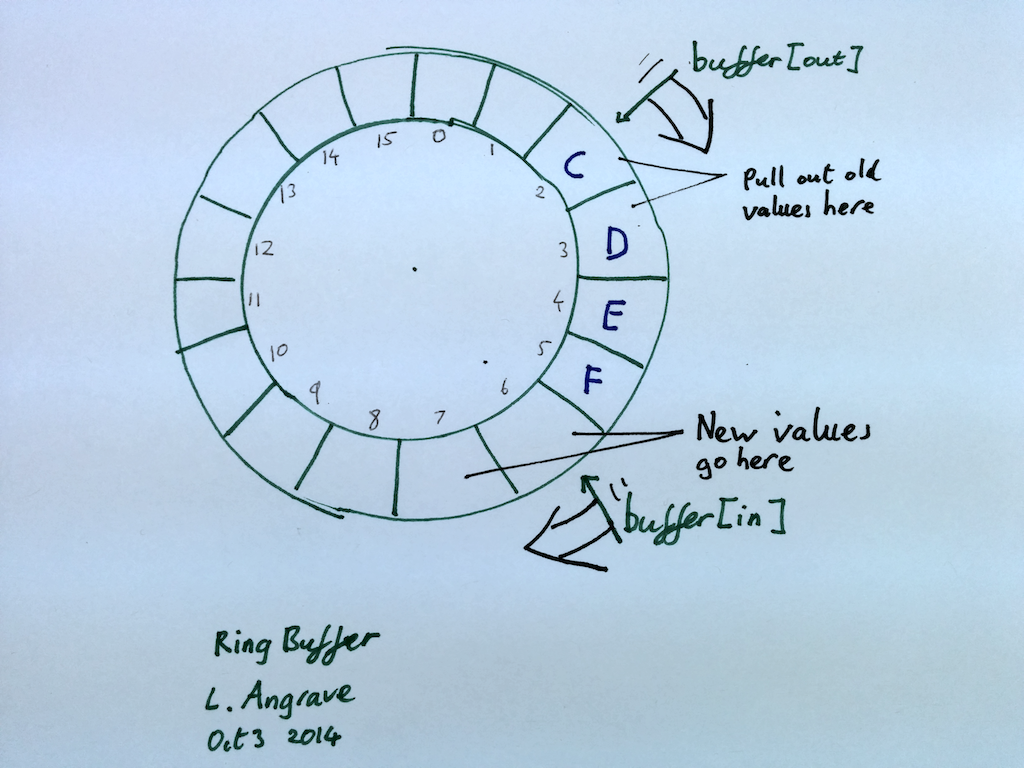
\includegraphics[width=.5\textwidth]{synchronization/images/ring_buffer.png}
\end{center}

A simple (single-threaded) implementation is shown below.
Note, enqueue and dequeue do not guard against underflow or overflow.
It's possible to add an item when when the queue is full and possible to remove an item when the queue is empty.
For example if we added 20 integers (1,2,3\ldots{}) to the queue and did not dequeue any items then values \keyword{17,18,19,20} would overwrite the \keyword{1,2,3,4}.
We won't fix this problem right now, instead when we create the multi-threaded version we will ensure enqueue-ing and dequeue-ing threads are blocked while the ring buffer is full or empty respectively.

\begin{lstlisting}[language=C]
void *buffer[16];
int in = 0, out = 0;

void enqueue(void *value) { /* Add one item to the front of the queue*/
  buffer[in] = value;
  in++; /* Advance the index for next time */
  if (in == 16) in = 0; /* Wrap around! */
}

void *dequeue() { /* Remove one item to the end of the queue.*/
  void *result = buffer[out];
  out++;
  if (out == 16) out = 0;
  return result;
}
\end{lstlisting}

\subsection{Ring Buffer Gotchas}

It's very tempting to write the enqueue or dequeue method in the following compact form.

\begin{lstlisting}[language=C]
  // N is the capacity of the buffer
void enqueue(void *value)
  b[ (in++) % N ] = value;
}
\end{lstlisting}

This method would appear to work (pass simple tests etc) but contains a subtle bug.
With enough enqueue operations (a bit more than two billion) the int value of \keyword{in} will overflow and become negative! The modulo (or `remainder') operator \keyword{\%} preserves the sign.
Thus you might end up writing into \keyword{b[-14]} for example!

A compact form is correct uses bit masking provided N is 2\^{}x (16,32,64,\ldots{})

\begin{lstlisting}[language=C]
b[ (in++) & (N-1) ] = value;
\end{lstlisting}

This buffer does not yet prevent buffer underflow or overflow.
For that, we'll turn to our multi-threaded attempt that will block a thread until there is space or there is at least one item to remove.

\subsection{Multithreaded Correctness}

The following code is an incorrect implementation.
What will happen?
Will \keyword{enqueue} and/or \keyword{dequeue} block?
Is mutual exclusion satisfied?
Can the buffer underflow?
Can the buffer overflow?
For clarity \keyword{pthread\_mutex} is shortened to \keyword{p\_m} and we assume sem\_wait cannot be interrupted.

\begin{lstlisting}[language=C]
#define N 16
void *b[N]
int in = 0, out = 0
p_m_t lock
sem_t s1,s2
void init() {
    p_m_init(&lock, NULL)
    sem_init(&s1, 0, 16)
    sem_init(&s2, 0, 0)
}

enqueue(void *value) {
    p_m_lock(&lock)

    // Hint: Wait while zero. Decrement and return
    sem_wait( &s1 )

    b[ (in++) & (N-1) ] = value

    // Hint: Increment. Will wake up a waiting thread
    sem_post(&s1)
    p_m_unlock(&lock)
}
void *dequeue(){
    p_m_lock(&lock)
    sem_wait(&s2)
    void *result = b[(out++) & (N-1) ]
    sem_post(&s2)
    p_m_unlock(&lock)
    return result
}
\end{lstlisting}

\subsection{Analysis}

Before reading on, see how many mistakes you can find. Then determine what would happen if threads called the enqueue and dequeue methods.

\begin{itemize}
\tightlist
\item
  The enqueue method waits and posts on the same semaphore (s1) and similarly with enqueue and (s2) i.e.~we decrement the value and then immediately increment the value, so by the end of the function the semaphore value is unchanged!
\item
  The initial value of s1 is 16, so the semaphore will never be reduced to zero - enqueue will not block if the ring buffer is full - so overflow is possible.
\item
  The initial value of s2 is zero, so calls to dequeue will always block and never return!
\item
  The order of mutex lock and sem\_wait will need to be swapped, however this example is so broken that this bug has no effect!
\end{itemize}

\subsection{Another Analysis}

The following code is an incorrect implementation.
What will happen?
Will \keyword{enqueue} and/or \keyword{dequeue} block?
Is mutual exclusion satisfied?
Can the buffer underflow?
Can the buffer overflow?
For clarity \keyword{pthread\_mutex} is shortened to \keyword{p\_m} and we assume sem\_wait cannot be interrupted.

\begin{lstlisting}[language=C]
void *b[16]
int in = 0, out = 0
p_m_t lock
sem_t s1, s2
void init() {
    sem_init(&s1,0,16)
    sem_init(&s2,0,0)
}

enqueue(void *value){
 sem_wait(&s2)
 p_m_lock(&lock)

 b[ (in++) & (N-1) ] = value

 p_m_unlock(&lock)
 sem_post(&s1)
}

void *dequeue(){
  sem_wait(&s1)
  p_m_lock(&lock)
  void *result = b[(out++) & (N-1)]
  p_m_unlock(&lock)
  sem_post(&s2)

  return result;
}
\end{lstlisting}

Here are a few problems that we hope you've found.

\begin{itemize}
\tightlist
\item
  The initial value of s2 is 0.
  Thus enqueue will block on the first call to sem\_wait even though the buffer is empty!
\item
  The initial value of s1 is 16.
  Thus dequeue will not block on the first call to sem\_wait even though the buffer is empty - Underflow!
  The dequeue method will return invalid data.
\item
  The code does not satisfy Mutual Exclusion.
  Two threads can modify \keyword{in} or \keyword{out} at the same time!
  The code appears to use mutex lock. Unfortunately the lock was never initialized with \keyword{pthread\_mutex\_init()} or \keyword{PTHREAD\_MUTEX\_INITIALIZER} - so the lock may not work (\keyword{pthread\_mutex\_lock} may simply do nothing)
\end{itemize}

\subsection{Correct implementation of a ring buffer}

As the mutex lock is stored in global (static) memory it can be initialized with \keyword{PTHREAD\_MUTEX\_INITIALIZER}.
If we had allocated space for the mutex on the heap, then we would have used \keyword{pthread\_mutex\_init(ptr, NULL)}

\begin{lstlisting}[language=C]
#include <pthread.h>
#include <semaphore.h>
// N must be 2^i
#define N (16)

void *b[N]
int in = 0, out = 0
p_m_t lock = PTHREAD_MUTEX_INITIALIZER
sem_t countsem, spacesem

void init() {
  sem_init(&countsem, 0, 0)
  sem_init(&spacesem, 0, 16)
}
\end{lstlisting}

The enqueue method is shown below.
Make sure to note.

\begin{enumerate}
\item The lock is only held during the critical section (access to the data structure).
\item A complete implementation would need to guard against early returns from \keyword{sem\_wait} due to POSIX signals.
\end{enumerate}

\begin{lstlisting}[language=C]
enqueue(void *value){
 // wait if there is no space left:
 sem_wait( &spacesem )

 p_m_lock(&lock)
 b[ (in++) & (N-1) ] = value
 p_m_unlock(&lock)

 // increment the count of the number of items
 sem_post(&countsem)
}
\end{lstlisting}

The \keyword{dequeue} implementation is shown below.
Notice the symmetry of the synchronization calls to \keyword{enqueue}.
In both cases, the functions first wait if the count of spaces or count of items is zero.

\begin{lstlisting}[language=C]
void *dequeue(){
  // Wait if there are no items in the buffer
  sem_wait(&countsem)

  p_m_lock(&lock)
  void *result = b[(out++) & (N-1)]
  p_m_unlock(&lock)

  // Increment the count of the number of spaces
  sem_post(&spacesem)

  return result
}
\end{lstlisting}

Food for thought:

\begin{itemize}
\tightlist
\item
  What would happen if the order of \keyword{pthread\_mutex\_unlock} and \keyword{sem\_post} calls were swapped?
\item
  What would happen if the order of \keyword{sem\_wait} and \keyword{pthread\_mutex\_lock} calls were swapped?
\end{itemize}


\section{Extra: Process Synchronization}

You thought that you were using different processes, so you don't have to synchronize?
Think again!
You may not have race conditions within a process but what if your process needs to interact with the system around it?
Let's consider a motivating example

\begin{lstlisting}[language=C]
void write_string(const char *data) {
    int fd = open("my_file.txt", O_WRONLY);
    write(fd, data, strlen(data));
    close(fd);
}

int main() {
    if(!fork()) {
        write_string("key1: value1");
        wait(NULL);
    } else {
        write_string("key2: value2");
    }
    return 0;
}
\end{lstlisting}

If none of the system calls fail then we should get something that looks like this given the file was empty to begin with.

\begin{lstlisting}
key1: value1
key2: value2
\end{lstlisting}

\begin{lstlisting}
key2: value2
key1: value1
\end{lstlisting}

\subsection{Interruption}

But, there is a hidden nuance.
Most system calls can be \keyword{interrupted} meaning that the operating system can stop an ongoing system call because it needs to stop the process.
So barring \keyword{fork} \keyword{wait} \keyword{open} and \keyword{close} from failing -- they typically go to completion -- what happens if \keyword{write} fails? If write fails and no bytes are written, we can get something like \keyword{key1: value1} or \keyword{key2: value2}.
This is data loss which is incorrect but won't corrupt the file.
What happens if write gets interrupted after a partial write? We get all sorts of madness.
For example,

\begin{lstlisting}
key2: key1: value1
\end{lstlisting}

\subsection{Solution}

You can create mutex before fork-ing - however the child and parent process will not share virtual memory and each one will have a mutex independent of the other.
Advanced note: There are advanced options using shared memory that allow a child and parent to share a mutex if it's created with the correct options and uses a shared memory segment.
See \href{http://stackoverflow.com/questions/19172541/procs-fork-and-mutexes}{stackoverflow example}

So what should we do? We should use a shared mutex! Consider the following code.

\begin{lstlisting}[language=C]
pthread_mutex_t * mutex = NULL;
pthread_mutexattr_t attr;

void write_string(const char *data) {
    pthread_mutex_lock(mutex);
    int fd = open("my_file.txt", O_WRONLY);
    int bytes_to_write = strlen(data), written = 0;
    while(written < bytes_to_write) {
        written += write(fd, data + written, bytes_to_write - written);
    }
    close(fd);
    pthread_mutex_unlock(mutex);
}

int main() {
    pthread_mutexattr_init(&attr);
    pthread_mutexattr_setpshared(&attr, PTHREAD_PROCESS_SHARED);
    pmutex = mmap (NULL, sizeof(pthread_mutex_t),
                PROT_READ|PROT_WRITE, MAP_SHARED|MAP_ANON, -1, 0);
    pthread_mutex_init(pmutex, &attrmutex);
    if(!fork()) {
        write_string("key1: value1");
        wait(NULL);
        pthread_mutex_destroy(pmutex);
        pthread_mutexattr_destroy(&attrmutex);
        munmap((void *)pmutex, sizeof(*pmutex));
    } else {
        write_string("key2: value2");
    }
    return 0;
}
\end{lstlisting}

What the code does in main is initialize a process shared mutex using a piece of \keyword{shared} memory.
You will find out what this call to \keyword{mmap} does later -- just assume for the time being that it create memory that is shared between processes.
We can initialize a \keyword{pthread\_mutex\_t} in that special piece of memory and use it as normal.
To counter \keyword{write} failing, we have put the \keyword{write} call inside a while loop that keeps writing so long as there are bytes left to write.
Now if all the other system calls function, there should be more more race conditions.

Most programs try to avoid this problem entirely by writing to separate files, but it is good to know that there are mutexes across processes, and they are useful.
You can use all of the primitives that you were taught previously! Barriers, semaphores, and condition variables can all be initialized on a shared piece of memory and used in similar ways to their multithreading counterparts.
You don't need to know the implementation, just need to know that mutexes and other synchronization primitives can be shared across processes and some of the benefits.

\begin{itemize}
\tightlist
\item
  You don't have to worry about arbitrary memory addresses becoming race condition candidates. This means that only areas that you specifically \keyword{mmap} or outside system resources like files are ever in danger.
\item
  You get the nice isolation of a processes so if one process fails the system can maintain intact
\item
  When you have a lot of threads, creating a process might ease the system load
\end{itemize}

\section{Extra: Higher Order Models of Synchronization}

When using atomics, you need to specify the right model of synchronization in order to make sure you have the correct behavior for your program.
You can read more about them \href{https://gcc.gnu.org/wiki/Atomic/GCCMM/AtomicSync}{On the gcc wiki}
These examples are adapted from those.

\subsection{Sequentially Consistent}

Sequentially consistent is the simplest, least error prone and most expensive model. This model says that any change that happens, all changes before it will be synchronized between all threads.

\begin{verbatim}
    Thread 1                    Thread 2
    1.0 atomic_store(x, 1)
    1.1 y = 10                  2.1 if (atomic_load(x) == 0)
    1.2 atomic_store(x, 0);     2.2    y != 10 && abort();
\end{verbatim}

Will never quit.
This is because either the store happens before the if statement in thread 2 and y == 1 or the store happens after and x does not equal 2.

\subsection{Relaxed}

Relaxed is a simple memory order providing for more optimizations.
This means that only a particular operation needs to be atomic.
One can have stale reads and writes, but after reading the new value, it won't become old.

\begin{verbatim}
    -Thread 1-              -Thread 2-
    atomic_store(x, 1);     printf("%d\n", x) // 1
    atomic_store(x, 0);     printf("%d\n", x) // could be 1 or 0
                            printf("%d\n", x) // could be 1 or 0
\end{verbatim}

But that means that previous loads and stores don't need to effect other threads.
In the previous example, the code can now fail.

\subsection{Acquire/Release}

The simplest way I can explain it is the order of atomic variables don't need to be consistent -- meaning if I assign atomic var y to be 10 then atomic var x to be 0 those don't need to propagate and you could get stale reads.
Non-atomic variables have to get updated in all threads though.

\subsection{Consume}

Imagine the same as above except non-atomic variables don't need to get updated in all threads.
This model was introduced so that there can be an Acquire/Release/Consume model without mixing in Relaxed because Consume is similar to relax.

\section{External Resources}

\begin{itemize}
\item \href{http://linux.die.net/man/3/pthread_mutex_lock}{pthread\_mutex\_lock man page}
\item \href{http://linux.die.net/man/3/pthread_mutex_unlock}{pthread\_mutex\_unlock man page}
\item \href{http://linux.die.net/man/3/pthread_mutex_init}{pthread\_mutex\_init man page}
\item \href{http://linux.die.net/man/3/pthread_mutex_destroy}{pthread\_mutex\_destroy man page}
\item \href{http://man7.org/linux/man-pages/man3/sem_init.3.html}{sem\_init}
\item \href{http://man7.org/linux/man-pages/man3/sem_wait.3.html}{sem\_wait}
\item \href{http://man7.org/linux/man-pages/man3/sem_post.3.html}{sem\_post}
\item \href{http://man7.org/linux/man-pages/man3/sem_destroy.3.html}{sem\_destroy}
\end{itemize}


\section{Topics}

\begin{itemize}
\tightlist
\item
  Atomic operations
\item
  Critical Section
\item
  Producer Consumer Problem
\item
  Using Condition Variables
\item
  Using Counting Semaphore
\item
  Implementing a barrier
\item
  Implementing a ring buffer
\item
  Using pthread\_mutex
\item
  Implementing producer consumer
\item
  Analyzing multi-threaded coded
\end{itemize}

\section{Questions}

\begin{itemize}
\tightlist
\item
  What is atomic operation?
\item
  Why will the following not work in parallel code

\begin{lstlisting}[language=C]
//In the global section
size_t a;
//In pthread function
for(int i = 0; i < 100000000; i++) a++;
\end{lstlisting}

  And this will?

\begin{lstlisting}[language=C]
//In the global section
atomic_size_t a;
//In pthread function
for(int i = 0; i < 100000000; i++) atomic_fetch_add(a, 1);
\end{lstlisting}
\item
  What are some downsides to atomic operations? What would be faster: keeping a local variable or many atomic operations?
\item
  What is the critical section?
\item
  Once you have identified a critical section, what is one way of assuring that only one thread will be in the section at a time?
\item
  Identify the critical section here

\begin{lstlisting}[language=C]
struct linked_list;
struct node;
void add_linked_list(linked_list *ll, void* elem){
    node* packaged = new_node(elem);
    if(ll->head){
         ll->head =
    }else{
         packaged->next = ll->head;
         ll->head = packaged;
         ll->size++;
    }

}

void* pop_elem(linked_list *ll, size_t index){
    if(index >= ll->size) return NULL;

    node *i, *prev;
    for(i = ll->head; i && index; i = i->next, index--){
        prev = i;
    }

    //i points to the element we need to pop, prev before
    if(prev->next) prev->next = prev->next->next;
    ll->size--;
    void* elem = i->elem;
    destroy_node(i);
    return elem;
}
\end{lstlisting}

\item How tight can you make the critical section?
\item What is a producer consumer problem? How might the above be a producer consumer problem be used in the above section? How is a producer consumer problem related to a reader writer problem?
\item What is a condition variable? Why is there an advantage to using one over a \keyword{while} loop?
\item Why is this code dangerous?

\begin{lstlisting}[language=C]
if(not_ready){
     pthread_cond_wait(&cv, &mtx);
}
\end{lstlisting}

\item
  What is a counting semaphore? Give me an analogy to a cookie jar/pizza box/limited food item.
\item
  What is a thread barrier?
\item
  Use a counting semaphore to implement a barrier.
\item
  Write up a Producer/Consumer queue, How about a producer consumer stack?
\item
  Give me an implementation of a reader-writer lock with condition variables, make a struct with whatever you need, it just needs to be able to support the following functions

\begin{lstlisting}[language=C]
void reader_lock(rw_lock_t* lck);
void writer_lock(rw_lock_t* lck);
void reader_unlock(rw_lock_t* lck);
void writer_unlock(rw_lock_t* lck);
\end{lstlisting}

  The only specification is that in between \keyword{reader\_lock} and \keyword{reader\_unlock}, no writers can write. In between the writer locks, only one writer may be writing at a time.
\item
  Write code to implement a producer consumer using ONLY three counting semaphores. Assume there can be more than one thread calling enqueue and dequeue. Determine the initial value of each semaphore.
\item
  Write code to implement a producer consumer using condition variables and a mutex. Assume there can be more than one thread calling enqueue and dequeue.
\item
  Use CVs to implement add(unsigned int) and subtract(unsigned int) blocking functions that never allow the global value to be greater than 100.
\item
  Use CVs to implement a barrier for 15 threads.
\item
  How many of the following statements are true?
\item
There can be multiple active readers
\item
There can be multiple active writers
\item
When there is an active writer the number of active readers must be zero
\item
If there is an active reader the number of active writers must be zero
\item
A writer must wait until the current active readers have finished
\end{itemize}

\bibliographystyle{plainnat}
\bibliography{synchronization/synchronization}

\chapter{Deadlock}

\epigraph{No, you can't always get what you want
\\You can't always get what you want
\\You can't always get what you want
\\But if you try sometime you find
\\You get what you need}{The philosophers Jagger \& Richards}

\gls{Deadlock} is defined as when a system cannot make and forward progress.
We define a system for the rest of the chapter as a set of rules by which a set of processes can move from one state to another, where a state is either working or waiting for a particular resource.
Forward progress is defined as if there is at least one process working or we can award a process waiting for a resource that resource.
In a lot of systems, Deadlock is just avoided by ignore the entire concept \cite[P.237]{silberschatz2006operating}.
Have you heard about turn it on and off again?
For products where the stakes are low (User Operating Systems, Phones), it may be more efficient not prevent deadlock.
But in the cases where ``failure is not an option'' - Apollo 13, you need a system that tracks and breaks deadlock or better yet prevents it entirely.
Apollo 13 may have not failed because of deadlock, but probably wouldn't be good to restart the system on liftoff.

Mission critical operating systems need this guarantee formally because playing the odds with people's lives isn't a good idea.
Okay so how do we do this? We model the problem.
Even though it is a common statistical phrase that all models are wrong, the more accurate the model is to the system the better chance that it'll work better.

\section{Resource Allocation Graphs}

\begin{figure}[H]
\centering
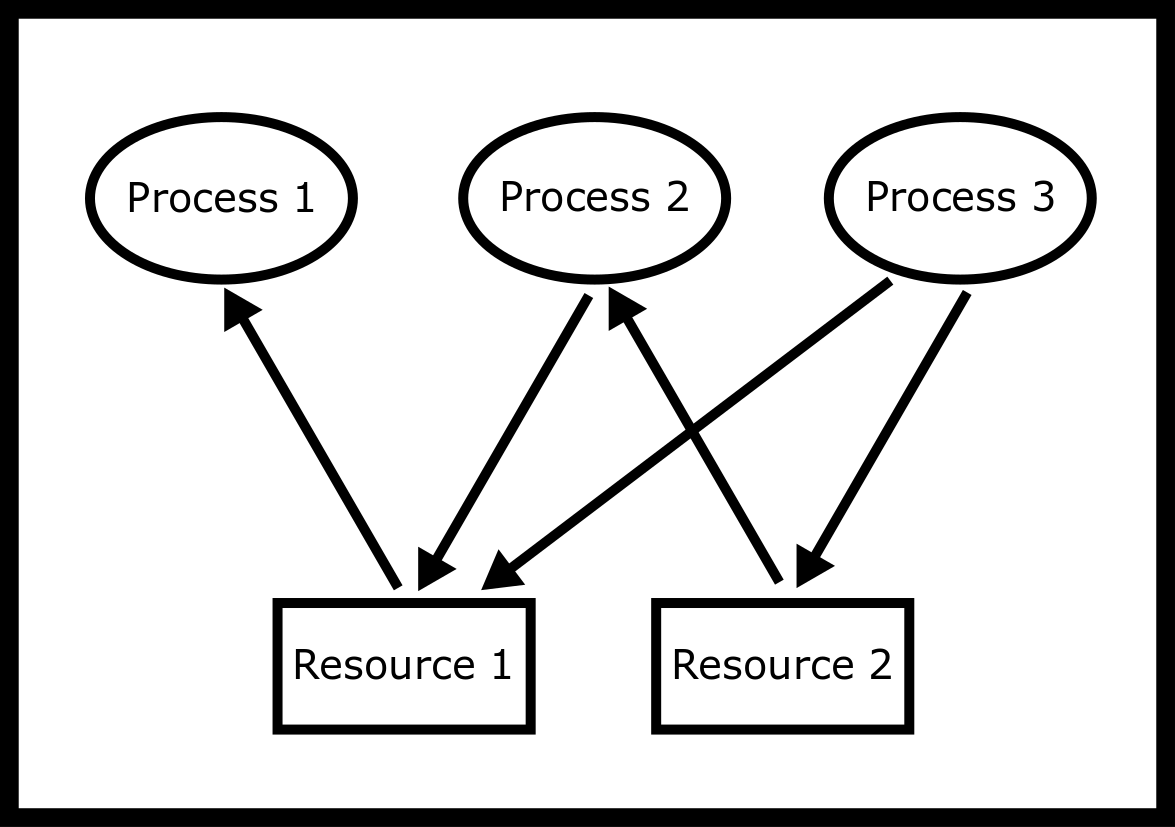
\includegraphics[width=.6\textwidth]{deadlock/drawings/rag.png}
\caption{Resource allocation graph}
\label{ragfigure}
\end{figure}


One such way is modeling the system with a resource allocation graph (\gls{RAG}).
A resource allocation graph tracks which resource is held by which process and which process is waiting for a resource of a particular type.
It is very powerful and simple tool to illustrate how interacting processes can deadlock.
If a process is \emph{using} a resource, an arrow is drawn from the resource node to the process node.
If a process is \emph{requesting} a resource, an arrow is drawn from the process node to the resource node.
If there is a cycle in the Resource Allocation Graph and each resource in the cycle provides only one instance, then the processes will deadlock.
For example, if process 1 holds resource A, process 2 holds resource B and process 1 is waiting for B and process 2 is waiting for A, then process 1 and 2 process will be deadlocked \ref{ragfigure}.
We can detect a deadlock by traversing the graph and searching for a cycle using graph traversal algorithm, such as the Depth First Search (DFS).
This graph is considered as a directed graph and we can treat both the processes and resources as nodes.

\begin{minted}{C}
typedef struct {
	int node_id; // Node in this particular graph
	Graph **reachable_nodes; // List of nodes that can be reached from this node
	int size_reachable_nodes; // Size of the List
} Graph;

// isCyclic() traverses a graph using DFS and detects whether it has a cycle
// isCyclic() uses a recursive approach
// G points to a node in a graph, can be either a resource or a process
// is_visited is an array indexed with node_id and initialized with zeroes(false) to record whether a particular node has been visited
int isCyclic(Graph *G, int* is_visited) {
	if (this graph has been visited) {
		// Oh! the cycle is found
		return true;
	} else {
		1. Mark this node as visited
		2. Traverse through all nodes in the reachable_nodes
		3. Call isCyclic() for each nodes
		4. Evaluate the return value of isCyclic()
	}
	// Nope, this graph does not have any cycle
	return false;
}
\end{minted}

\begin{figure}[H]
\centering
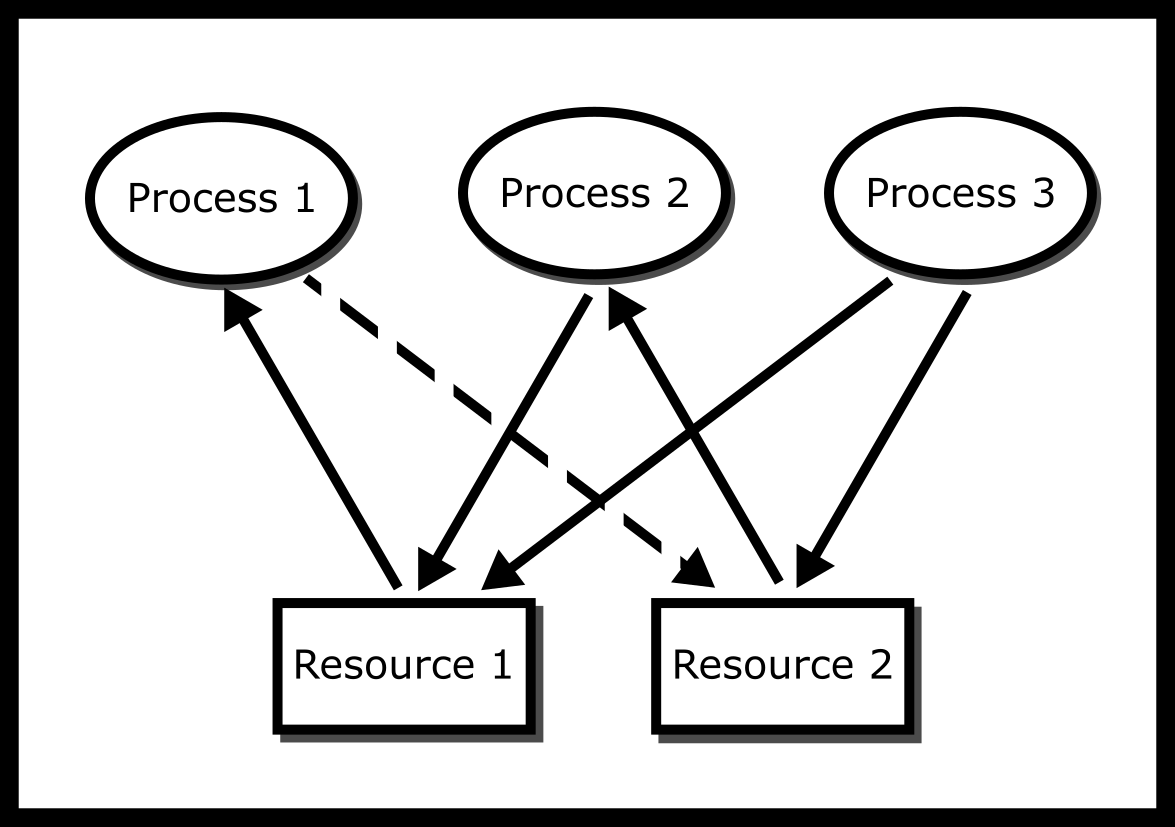
\includegraphics[width=.5\textwidth]{deadlock/drawings/deadlock.png}
\caption{Graph based Deadlock}
\end{figure}

\section{Coffman conditions}

Assume that the processes ask for exclusive access to the file.
If you have a bunch of processes running and they request resources and the operating system ends up in this state, you deadlock!
You may not see this because the operating system may \textbf{preempt} some processes breaking the cycle but there is still a change that your three lonely processes could deadlock.
You can also make these kind of graphs with \keyword{make} and rule dependencies with our Parallel Make MP for example.

There are four \emph{necessary} and \emph{sufficient} conditions for deadlock -- meaning if these conditions hold then there is a non-zero probability that the system will deadlock at any given iteration.
These are known as the \gls{Coffman Conditions} \cite{coffman1971system}.

\begin{itemize}
\tightlist
\item
  \gls{Mutual Exclusion}: no two processes can obtain a resource at the same time.
\item
  \gls{Circular Wait}: there exists a cycle in the Resource Allocation Graph, or there exists a set of processes \{P1,P2,\ldots{}\} such that P1 is waiting for resources held by P2, which is waiting for P3,\ldots{}, which is waiting for P1.
\item
  \gls{Hold and Wait}: a process once obtaining a resource does not let go.
\item
  No \gls{pre-emption}: nothing can force the process to give up a resource.
\end{itemize}

\begin{proof} Deadlock can happen if and only if the four Coffman conditions are satisfied.

$\rightarrow$ If the system is deadlocked, the four Coffman conditions are apparent.

\begin{itemize}
\item For the purposes of contradiction, assume that there is no circular wait. If not then that means the resource allocation graph is acyclic, meaning that there is at least one one process that is not waiting on any resource to be freed. Since the system can move forward, the system is not deadlocked.
\item For the purposes of contradiction, assume that there is no mutual exclusion. If not, that means that no process is waiting on any other process for a resource. This breaks circular wait and the previous argument proves correctness.
\item For the purposes of contradiction, assume that processes don't hold and wait but our system still deadlocks. Since we have circular wait from the first condition at least one process must be waiting on another process. If that and processes don't hold and wait, that means one process must let go of a resource. Since the system has moved forward, it cannot be deadlocked.
\item For the purposes of contradiction, assume that we have preemption, but the system cannot be un-deadlocked. Have one process, or create one process, that recognizes the circular wait that must be apparent from above and break on the of the links. By the first branch, we must not have deadlock.
\end{itemize}

$\leftarrow$ If the four conditions are apparent, the system is deadlocked.
We will prove that if the system is not deadlocked, the four conditions are not apparent.
Though this proof is not formal, let us build a system with the three requirements not including circular wait.
Let assume that there is a set of processes $P = \{p_1, p_2, ..., p_n\}$ and there is a set of resources $R = \{r_1, r_2, ..., r_m\}$.
For simplicity, a process can only request one resource at a time but the proof can be generalized to multiple.
Let assume that the system is at different states at different times $t$.
Let us assume that the state of the system is a tuple $(h_t, w_t)$ where there are two function $h_t: R \rightarrow P \cup \{\text{unassigned}\}$ that maps resources to the processes that own them (this is a function, meaning that we have mutual exclusion) and or unassigned and $w_t: P \rightarrow R \cup \{\text{satisfied}\}$ that maps the requests that each process makes to a resource or if the process is satisfied.
Let $L_t \subseteq P \times R$ be a set of list of requests that a process uses to release a resource at any given time.
The evolution of the system is at each step at every time.

\begin{itemize}
\item Release all resources in $L_t$.
\item Find a process that is requesting a resource
\item If that resource is available give it to that process, generating a new $(h_{t+1}, w_{t+1})$ and exit the current iteration.
\item Else find another process and try the same resource allocation procedure in the previous step.
\end{itemize}

If all processes have been surveyed and none updates the system, consider it deadlocked.
More formally, this system is deadlocked means  if $\exists t_0, \forall t \geq t_0, \forall p \in P, w_t(p) \neq \text{satisfied} \text{ and } \exists q, q \neq p \rightarrow h_t(w_t(p)) = q$ (which is what we need to prove).

\begin{proof} These conditions imply deadlock.
  Deadlock for a system is defined as no work can be done now or later.
  Work can be done if a process is satisfied, or we can release a resource to a process.
  No process is satisfied by definition.
  Since the system can't preempt and release resources (by no preemption), the processes have to do it themselves.
  If the processes has a resource, it will not let it go until after it is satisfied by hold and wait.
  All resources requested by the processes are owned by other processes meaning that no process will let any resource go.
  Since we have shown no processes will give up a resource and no process is satisfied, the system is in deadlock.
\todo{Formalize Subproof}
\end{proof}
The last condition to address is circular wait.
Circular wait means that there exists $\forall p \in P, w_t(p) \neq \text{satisfied} \text{ and } \exists q, q \neq p \rightarrow h_t(w_t(p)) = q$.
Which is what we needed to show.
\end{proof}

If you break any of them, you cannot have deadlock! Consider the scenario where two students need to write both pen and paper and there is only one of each. Breaking mutual exclusion means that the students share the pen and paper. Breaking circular wait could be that the students agree to grab the pen then the paper. As a proof by contradiction, say that deadlock occurs under the rule and the conditions. Without loss of generality, that means a student would have to be waiting on a pen while holding the paper and the other waiting on a pen and holding the paper. We have contradicted ourselves because one student grabbed the paper without grabbing the pen, so deadlock must not be able to occur. Breaking hold and wait could be that the students try to get the pen and then the paper and if a student fails to grab the paper then they release the pen. This introduces a new problem called \textit{livelock} which will be discussed latter. Breaking preemption means that if the two students are in deadlock the teacher can come in and break up the deadlock by giving one of the students one the held on items or tell both students to put the items down.

\gls{livelock} relates to deadlock but it is not exactly deadlock.
Consider the breaking hold and wait solution as above.
Though deadlock is avoided, if we pick up the same device (a pen or the paper) again and again in the exact same pattern, neither of us will get any writing done.
More generally, livelock happens when the process looks like it is executing but no meaningful work is done.
Livelock is generally harder to detect because the processes generally look like they are working to the outside operating system whereas in deadlock the operating system generally knows when two processes are waiting on a system wide resource.
Another problem is that there are necessary conditions for livelock (i.e. deadlock does not occur) but not sufficient conditions -- meaning there is no set of rules where livelock has to occur.
You must formally prove in a system by what is known as an invariant.
One has to enumerate each of the steps of a system and if each of the steps eventually -- after some finite number of steps -- leads to forward progress, the system is not livelocked.
There are even better systems that prove bounded waits; a system can only be livelocked for at most $n$ cycles which may be important for something like stock exchanges.


\section{Approaches to solving deadlock}

Ignoring deadlock is the most obvious approach that started the chapter out detailing.
Quite humorously, the name for this approach is called the \gls{ostrich algorithm}.
Though there is no apparent source, the idea for the algorithm comes from the concept of an ostrich sticking its head in the sand.
When the operating system detects deadlock, it does nothing out of the ordinary and hopes that the deadlock goes away.
Now this is a slight misnomer because the operating system doesn't do anything \textit{abnormal} -- it is not like an operating system deadlocks every few minutes because it runs ~100 processes all requesting shared libraries.
An operating system still preempts processes when stopping them for context switches.
The operating system has the ability to interrupt any system call, potentially breaking a deadlock scenario.
The OS also makes some files read-only thus making the resource shareable.
What the algorithm refers to is that if there is an adversary that specifically crafts a program -- or equivalently a user who poorly writes a program -- that deadlock could not be caught by the operating system.
For everyday life, this tends to be fine.
When it is not we can turn to the following method.


Deadlock detection allows the system to enter a deadlocked state.
After entering, the system uses the information that it has to break deadlock.
As an example, consider multiple processes accessing files.
The operating system is able to keep track of all of the files/resources through file descriptors at some level either abstracted through an API or directly.
If the operating system detects a directed cycle in the operating system file descriptor table it may break one process' hold through scheduling for example and let the system proceed.
Why this is a popular choice in this realm is that there is no way of knowing which resources a program will select without running the program.
This is an extension of Rice's theorem \cite{rice} that says that we cannot know any semantic feature without running the program (semantic meaning like what files it tries to open).
So theoretically, it is sound.
The problem then gets introduced that we could reach a livelock scenario if we preempt a set of resources again and again.
The way around this is mostly probabilistic.
The operating system chooses a random resource to break hold and wait.
Now even though a user can craft a program where breaking hold and wait on each resource will result in a livelock, this doesn't happen as often on machines that run programs in practice or the livelock that does happen happens for a couple of cycles.
These kind of systems are good for products that need to maintain a non-deadlocked state but can tolerate a small chance of livelock for a short period of time.
The following proof \textbf{is not required for our 241 related purposes but is included for concreteness}.


\begin{comment}
\begin{proof}
  That livelock terminates with high probability.
  This meaning that for any probability level $l$ we can produce a number of iterations $n$ that the probability that the system is not livelocked after that state is at least $l$.

  Let $L = \{p_1, p_2, p_3, ...\}$ be an infinite set that has probabilities if we choose a resource that causes livelock in the $i$th iteration of the livelocked by breaking a random resource.
  Also let the set have the property that $\forall i > 0, \exists j > i, p_j < 1$ Meaning that for all elements after any given element that there is at least one element int he future that has a probability of breaking deadlock.
  The probability that the system is not livelocked after $n$ iterations is
\[
P(n) = 1 - \prod\limits_{i = 1}^{n}p_i
\]
Consider the new set $E = \{s_1, s_2, s_3, ...\}$ obtained by selecting all non-one elements. The set must be infinite by our sets property. It is easy to show that
\[
\prod\limits_{i = 1}^{n}p_i = \prod\limits_{i = 1}^{n}s_i
\]
And since
\[
P(n) = 1 - \prod\limits_{i = 1}^{n}s_i
\]
is a strictly monotonically decreasing function, it must pass the threshold for the probability level at some point. More rigorously
\begin{align*}
Y =& \sup E \\
\prod\limits_{i = 1}^{n}s_i <& Y^n \\
1 - \prod\limits_{i = 1}^{n}s_i >& 1 - Y^n \\
P(n) >& 1 - Y^n \\
P(n) >& l \\
1 - Y^n  >& l \\
\log_Y(1 - l) <& n
\end{align*}
We have found the number of steps in the set $E$ and since our set has the property that gaps between non-one elements is finite, we can reconstruct the number of iterations by picking an $n$ that satisfies the $E$ criteria and just adding the finite gaps together, which is what we needed to show.
\end{proof}
\end{comment}

Deadlock prevention is making sure that deadlock cannot happen, meaning that you break a Coffman condition.
This works the best inside a single program and the software engineer making the choice to break a certain Coffman condition. Consider the 
\href{https://en.wikipedia.org/wiki/Banker's\_algorithm}{Banker's Algorithm} \cite{Dijkstra:1965:CSP:1102034}.
It is another algorithm for deadlock avoidance.
The whole implementation is outside the scope of this class, just know that there are more generalized algorithms for operating systems.

\subsection{Extra: Banker's Algorithm}

The banker algorithm is actually not too complicated.
We can start out with the single resource solution.
Let's say that I'm a banker.
As a banker I have a finite amount of money.
As having a finite amount of money, I want to make loans and eventually get my money back.
Let's say that we have a set of $n$ people where each of them have a set amount or a limit $a_i$ ($i$ being the $i$th process) that they need to obtain before they can do any work.
I keep track in my book how much I've given to each person $l_i$, and I have some amount of principle $p$ at any given time.
For people to request money, they do the following. Consider the state of the system $(A=\{a_1, a_2, ...\}, L=\{l_1, l_2, ...\}, p)$.
An assumption of this system is that we have $p > \inf a_i$, or we have enough money to satisfy one person.
Also, each person will work for a finite period of time and give back our money.

\begin{itemize}
\item A person $j$ requests $m$ from me
\begin{itemize}
\item if $m < p$, they are denied.
\item if $m + l_j > a_i$ they are denied
\item Pretend we are in a new state $(A=\{..., a_j, ...\}, L=\{.., l_j + m, ...\}, p - m)$ where the process is granted the resource.
\end{itemize}
\item if now person $j$ is either satisfied ($l_j == a_j$) or $\exists i, a_j - l_j < p$. In other words we have enough money to satisfy one other person. If either, consider the transaction safe and give them the money.
\end{itemize}

Why does this work? Well at the start we are in a safe state -- defined by we have enough money to satisfy at least one person.
Each of these "loans" results in a safe state.
If we have exhausted our reserve, one person is working and will give us money greater than or equal to our previous "loan", thus putting us in a safe state again.
Since we always have the ability to make one additional move the system can never deadlock.
Now, there is no guarantee that the system won't livelock.
If the process we hope to request something never does, no work will be done -- but not due to deadlock.
This analogy expands to higher orders of magnitude but requires that either a process can do its work entirely or there exists a process whose combination of resources can be satisfied, which makes the algorithm a little more tricky (an additional for loop) but nothing too bad.
There are a fair bit of downsides to this though

\begin{itemize}
\item The program first needs to know how much of each resource a process needs. A lot of times that is impossible or the process requests the wrong amount because the programmer didn't foresee it.
\item The system could livelock.
\item We know in most systems that resources are generally not homogenous. Of course there are things like pipes and sockets but for the most part there is only 1 of a particular file. This could mean that the runtime of the algorithm could be slow for systems with millions of resources.
\item Also, this can't keep track of resources that come and go. A process may delete a resource as a side effect or create a resource. The algorithm assumes a static allocation and that each process performs a non-destructive operation.
\end{itemize}

\section{Dining Philosophers}

The Dining Philosophers problem is a classic synchronization problem.
Imagine I invite $n$ (let's say 6) philosophers to a meal.
We will sit them at a table with 6 chopsticks, one between each philosopher.
A philosopher alternates between wanting to eat or think.
To eat the philosopher must pick up the two chopsticks either side of their position.
The original problem required each philosopher to have two forks, but one can eat with a single fork so we rule this out.
However these chopsticks are shared with his neighbor.

\begin{figure}[H]
\centering
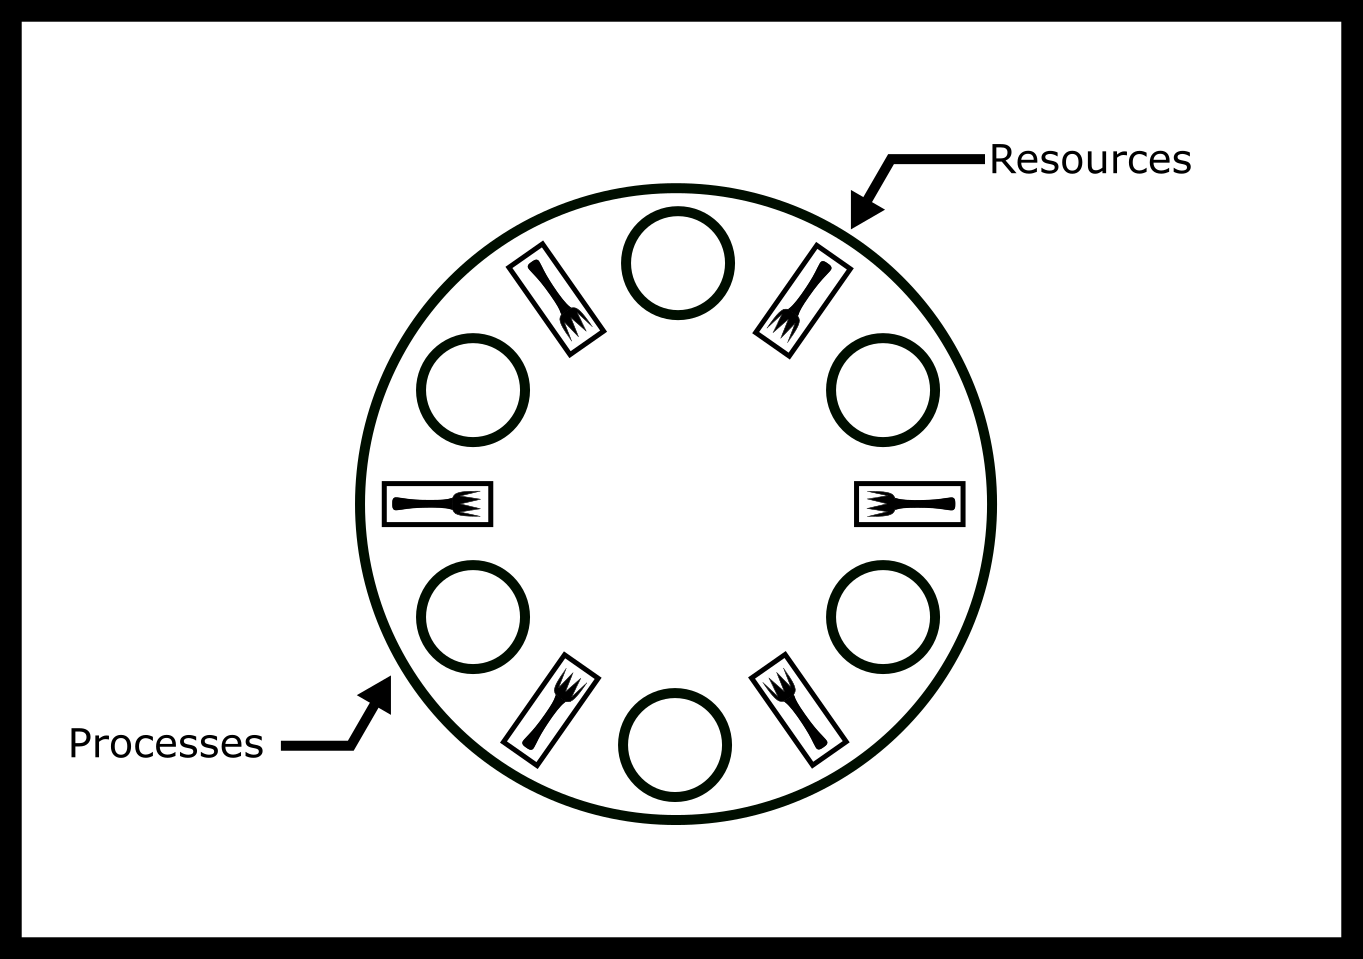
\includegraphics[width=.5\textwidth]{deadlock/drawings/dining.png}
\caption{Dining Philosophers}
\end{figure}

Is it possible to design an efficient solution such that all philosophers get to eat?
Or, will some philosophers starve, never obtaining a second chopstick?
Or will all of them deadlock?
For example, imagine each guest picks up the chopstick on their left and then waits for the chopstick on their right to be free.
Oops - our philosophers have deadlocked!
Each of the philosophers are essentially the same, meaning that each philosopher has the same instruction set based on the other philosopher i.e. you can't tell every even philosopher to do one thing and every odd philosopher to do another thing.


\subsection{Failed Solutions}

\begin{lstlisting}[language=C]
void* philosopher(void* forks){
     info phil_info = forks;
     pthread_mutex_t* left_fork = phil_info->left_fork;
     pthread_mutex_t* right_fork = phil_info->right_fork;
     while(phil_info->simulation){
          pthread_mutex_lock(left_fork);
          pthread_mutex_lock(right_fork);
          eat(left_fork, right_fork);
          pthread_mutex_unlock(left_fork);
          pthread_mutex_unlock(right_fork);
     }
}
\end{lstlisting}

This looks good but.
What if everyone picks up their left fork and is waiting on their right fork? We have deadlocked the program.
It is important to note that deadlock doesn't happen all the time and the probability that this solution deadlocks goes down as the number of philosophers goes up.
What is really important to note is that eventually that this solution will deadlock, letting threads starve which is bad.
Here is a simple resource allocation graph that shows how the system could be deadlocked

\begin{figure}[H]
\centering
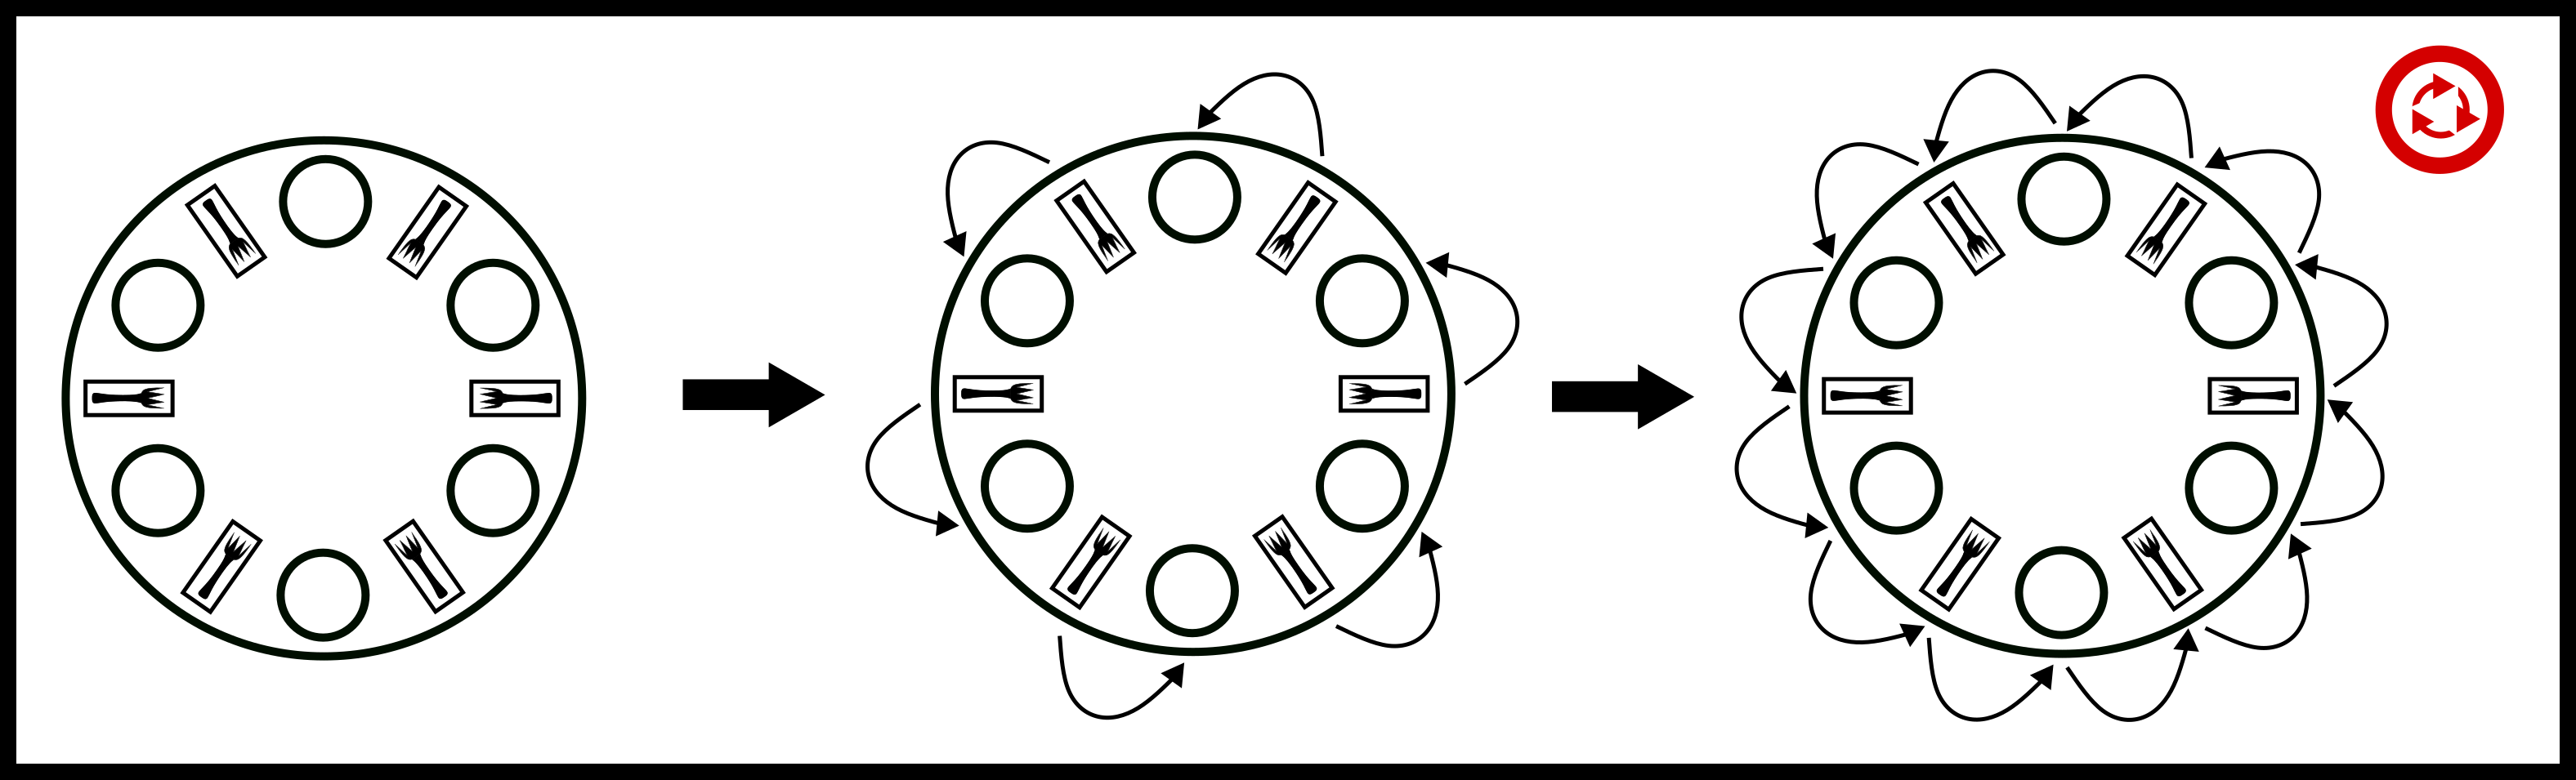
\includegraphics[width=.9\textwidth]{deadlock/drawings/dining_naive.png}
\caption{Left right dining philosopher cycle}
\end{figure}


So now you are thinking about breaking one of the Coffman conditions.
Let's break Hold and Wait!

\begin{lstlisting}[language=C]
void* philosopher(void* forks){
     info phil_info = forks;
     pthread_mutex_t* left_fork = phil_info->left_fork;
     pthread_mutex_t* right_fork = phil_info->right_fork;
     while(phil_info->simulation){
          int left_succeed = pthread_mutex_trylock(left_fork);
          if (!left_succeed) {
              sleep();
              continue;
          }
          int right_succeed = pthread_mutex_trylock(right_fork);
          if (!right_succeed) {
              pthread_mutex_unlock(left_fork);
              sleep();
              continue;
          }
          eat(left_fork, right_fork);
          pthread_mutex_unlock(left_fork);
          pthread_mutex_unlock(right_fork);
     }
}
\end{lstlisting}

Now our philosopher picks up the left fork and tries to grab the right.
If it's available, they eat.
If it's not available, they put the left fork down and try again.
No deadlock! But, there is a problem.
What if all the philosophers pick up their left at the same time, try to grab their right, put their left down, pick up their left, try to grab their right\ldots{}.
Here is what a time evolution of the system would look like.

\begin{figure}[H]
\centering
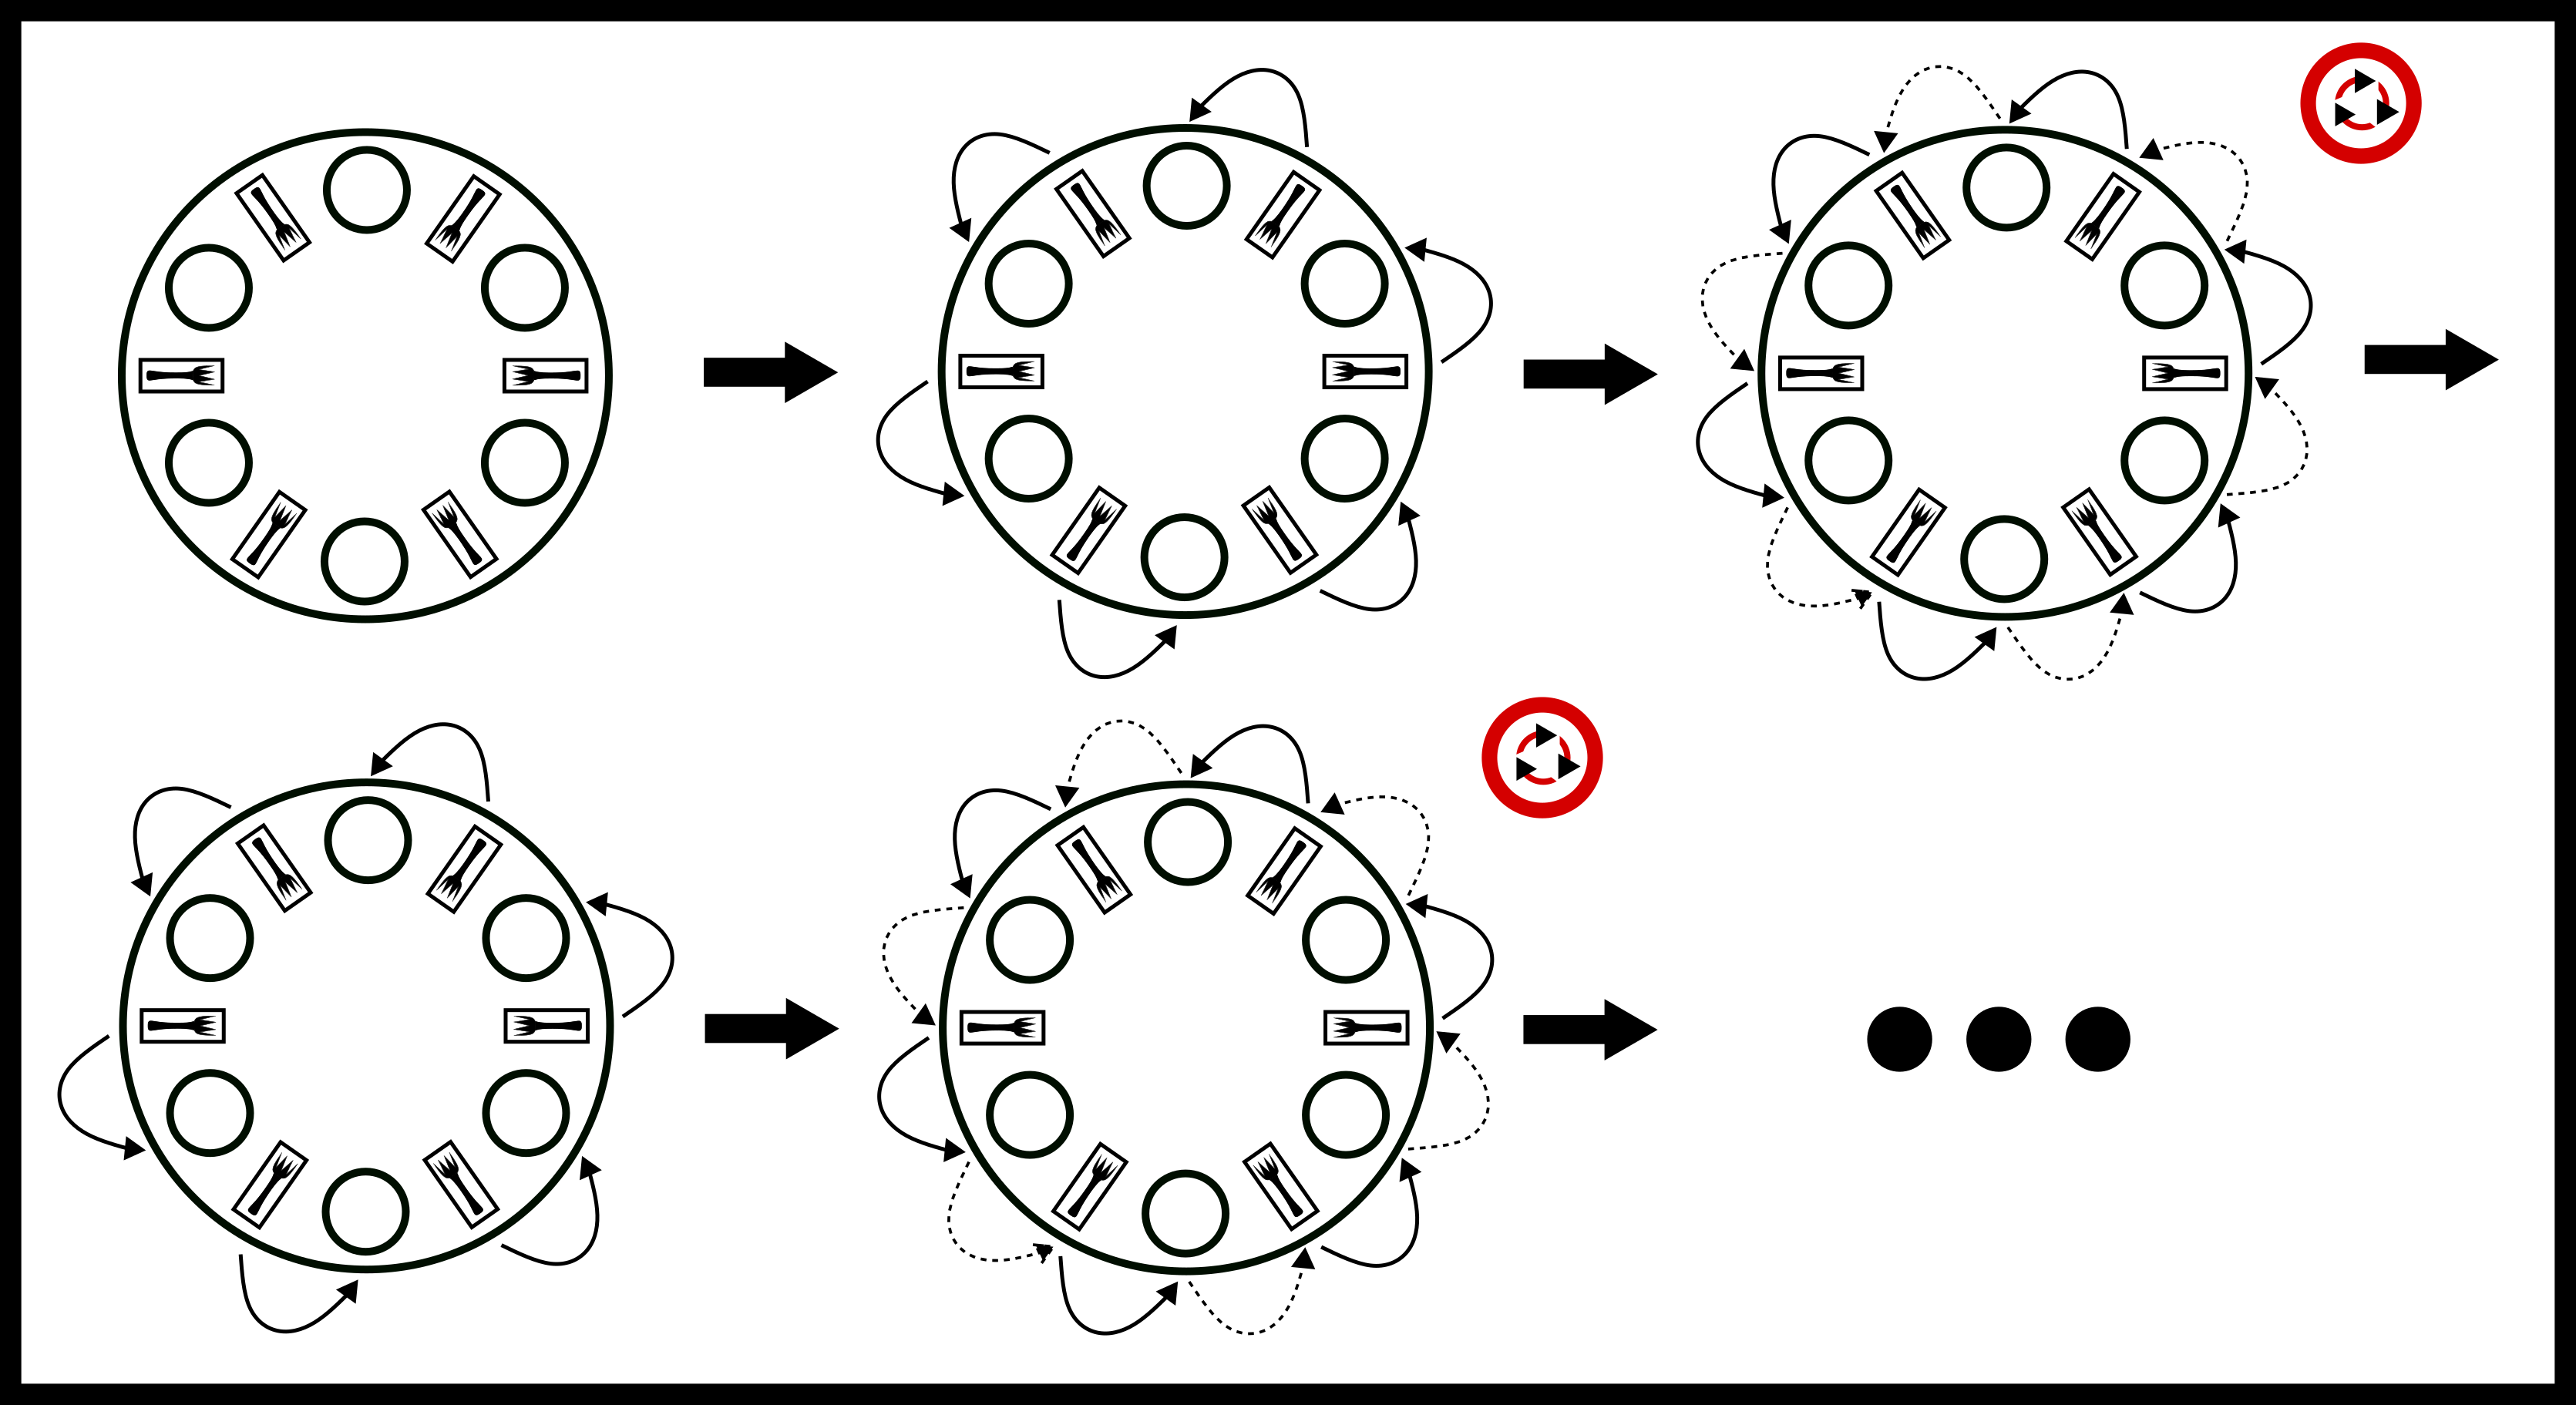
\includegraphics[width=.9\textwidth]{deadlock/drawings/dining_livelock.png}
\caption{Livelock Failure}
\end{figure}

We have now livelocked our solution! Our poor philosopher are still starving, so let's give them some proper solutions.

\section{Viable Solutions}

The naive arbitrator solution is have one arbitrator a mutex for example.
Have each of the philosopher ask the arbitrator for permission to eat or trylock an arbitrator mutex.
This solution allows one philosopher to eat at a time.
When they are done, another philosopher can ask for permission to eat.
This prevents deadlock because there is no circular wait! No philosopher has to wait on any other philosopher.
The advanced arbitrator solution is to implement a class that determines if the philosopher's forks are in the arbitrator's possession.
If they are, they give them to the philosopher, let him eat, and take the forks back.
This has the added bonus of being able to have multiple philosopher eat at the same time.

There are a lot of problems with these solutions.
One is that they are slow and have a single point of failure or the arbitrator.
Assuming that all the philosophers are good-willed, the arbitrator needs to be fair and be able to determine if a transaction would cause deadlock in the multi-arbitrator case.
Furthermore in practical systems, the arbitrator tends to give forks to the same processes because of scheduling or pseudo-randomness.
Another important thing to note is that this prevents deadlock for the entire system.
But in our model of dining philosophers, the philosopher has to release the lock themselves.
Then you can consider the case of the malicious philosopher (let's say Descartes because of his Evil Demons) could hold on to the arbitrator forever.
He would make forward progress and the system would make forward progress but there is no way of ensuring that each process makes forward progress without assuming something about the processes or having true preemption -- meaning that a higher authority (let's say Steve Jobs) tells them to stop eating forcibly.


\begin{proof} Arbitrator doesn't deadlock

The proof is about as simple as it gets. For number of philosophers $n >= 2$ only one philosopher can request resources at a time. There is no way to make a cycle in the resource allocation graph with only one philosopher acting in pickup the left then the right fork which is what we needed to show.

\end{proof}

\begin{figure}[H]
\centering
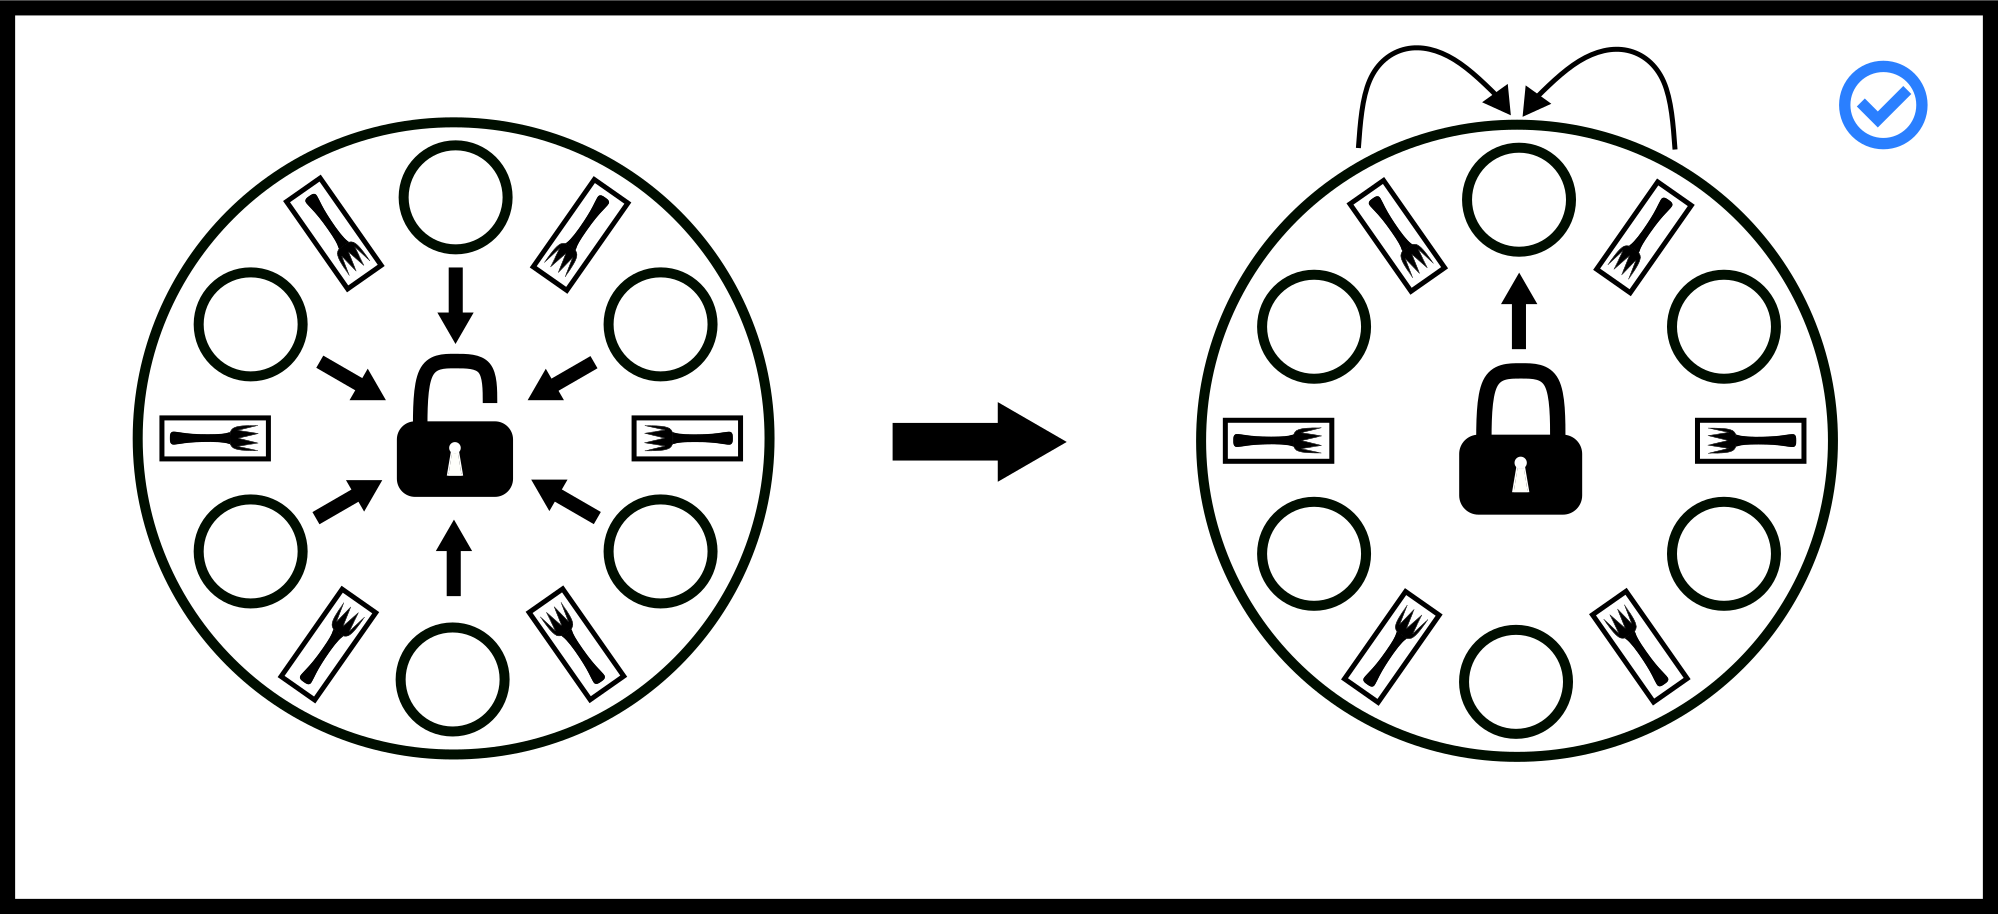
\includegraphics[width=.9\textwidth]{deadlock/drawings/dining_arbitrator.png}
\caption{Arbitrator Diagram}
\end{figure}

\subsection{Leaving the Table (Stallings' Solution)}

Why does the first solution deadlock?
Well there are $n$ philosophers and $n$ chopsticks.
What if there is only 1 philosopher at the table?
Can we deadlock?
No.
How about 2 philosophers?
3? \ldots{} You can see where this is going.
Stallings' \cite[P. 280]{stalling} solutions says to remove philosophers from the table until deadlock is not possible -- think about what the magic number of philosophers at the table.
The way to do this in actual system is through semaphores and letting a certain number of philosopher through.
This has the benefit that multiple philosophers can be eating.

In the case that the philosophers aren't evil, this solution requires a lot of time-consuming context switching.
There is also no reliable way to know the number of resources before hand.
In the dining philosophers case, this is solved because everything is known but trying to specify and operating system where you don't know which file is going to get opened by what process leads you with a faulty solution.
And again since semaphores are system constructs, they obey system timing clocks which means that the same processes tend to get added back into the queue again.
Now if a philosopher becomes evil, then the problem becomes that there is no preemption.
A philosopher can eat for as long as they want and the system will continue to function but that means the fairness of this solution can be low in the worst case.
This works best with timeouts or forced context switches in order to ensure bounded wait times.

\begin{proof} Stallings' Solution Doesn't Deadlock.
  Let's number the philosophers $\{p_0, p_1, .., p_{n-1}\}$ and the resources $\{r_0, r_1, .., r_{n-1}\}$.
  A philosopher $p_i$ needs resource $r_{i-1 \mod n}$ and $r_{i + 1 \mod n}$.
  Without loss of generality, let us take $p_i$ out of the picture.
  Each resource had exactly two philosophers that could use it.
  Now resources $r_{i-1 \mod n}$ and $r_{i + 1 \mod n}$ only have on philosopher waiting on it.
  Even if hold and wait, no preemption, and mutual exclusion or present, the resources can never enter a state where one philosopher requests them and they are held by another philosopher because only one philosopher can request them.
  Since there is no way to generate a cycle otherwise, circular wait cannot hold.
  Since circular wait cannot hold, deadlock cannot happen.
\end{proof}

Here is a visualization of the worst-case.
The system is about to deadlock, but the approach resolves it.

\begin{figure}[H]
\centering
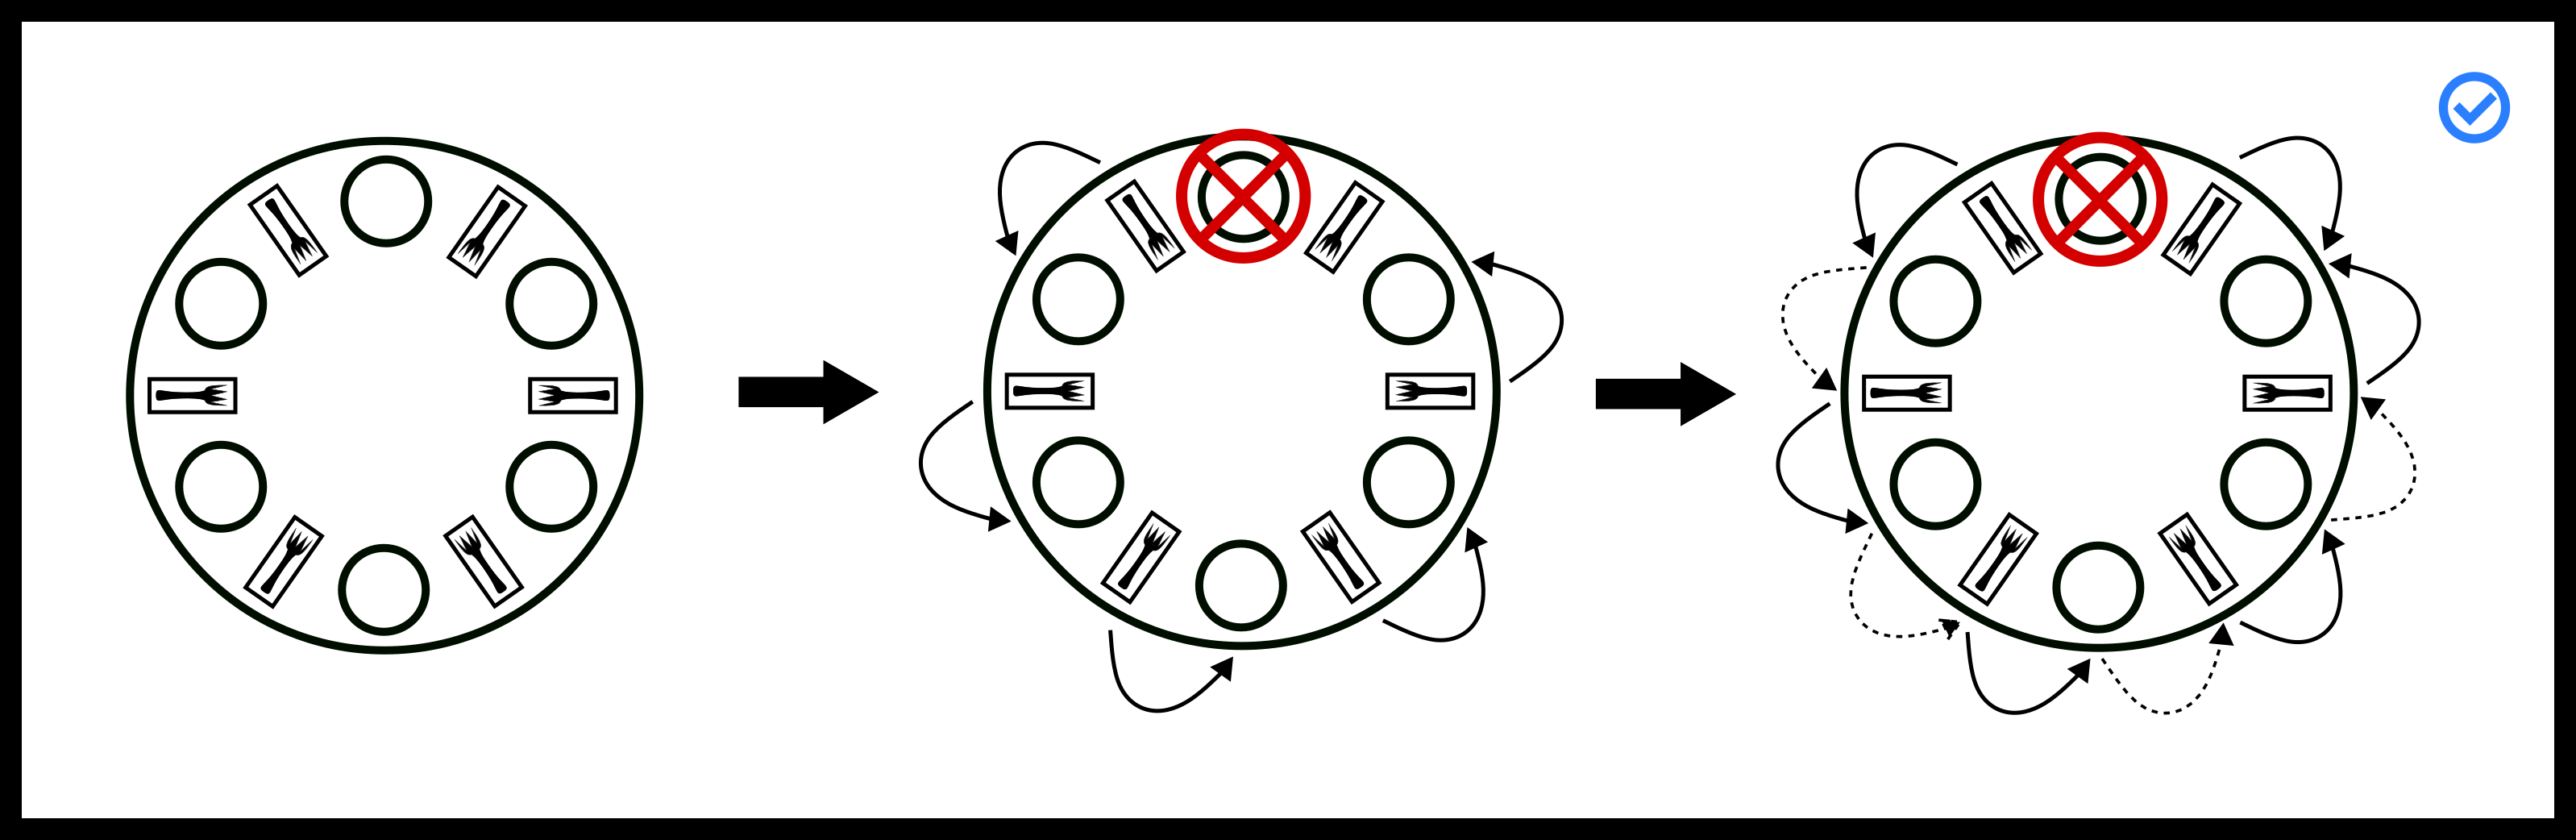
\includegraphics[width=.9\textwidth]{deadlock/drawings/dining_stalling.png}
\caption{Stalling solution almost deadlock}
\end{figure}


\subsection{Partial Ordering (Dijkstra's Solution)}

This is Dijkstra's solution \cite[P. 20]{EWD:EWD310}. He was the one to propose this problem on an exam.
Why does the first solution deadlock? Dijkstra thought that the last philosopher who picks up his left fork (causing the solution to deadlock) should pick up his right.
He accomplishes it by number the forks $1..n$, and tells each of the philosopher to pick up his lower number fork.
Let's run through the deadlock condition again.
Everyone tries to pick up their lower number fork first.
Philosopher $1$ gets fork $1$, Philosopher $2$ gets fork $2$, and so on until we get to Philosopher $n$.
They have to choose between fork $1$ and $n$.
fork $1$ is already held up by philosopher $1$, so they can't pick up that fork, meaning he won't pick up fork $n$.
We have broken circular wait! Meaning deadlock isn't possible.

The problems to this is that an entity either needs to know the finite set of resources or be able to produce a consistent partial order suck that circular wait cannot happen.
This also implies that there needs to be some entity, either the operating system or another process, deciding on the number and all of the philosophers need to agree on the number as new resources come in.
As we have also see with previous solutions, this relies on context switching so this prioritizes philosophers that have already eaten but can be made more fair by introducing random sleeps and waits.

\begin{proof} Dijkstra's Solution Doesn't Deadlock

The proof is very similar to the previous proof.
Let's number the philosophers $\{p_0, p_1, .., p_{n-1}\}$ and the resources $\{r_0, r_1, .., r_{n-1}\}$.
A philosopher $p_i$ needs resource $r_{i-1 \mod n}$ and $r_{i + 1 \mod n}$.
Each philosopher will grab $r_{i-1 \mod n}$ then $r_{i + 1 \mod n}$ but the last philosopher will grab in the reverse order.
Even if hold and wait, no preemption, and mutual exclusion or present.
Since the last philosopher will grab $r_{n-1}$ then $r_0$ there are two cases either the philosopher has the first lock or the philosopher doesn't.

If the last philosopher $p_{n-1}$ holds the first lock that means that the previous philosopher $p_{n-2}$ is waiting on $r_{n-1}$ meaning $r_{n-2}$ is available.
Since no other blockers, the philosopher previous $p_{n-3}$ will grab her first lock.
This is now a reduction to the previous proof of stalling because we now have $n$ resources but only $n-1$ philosophers, meaning this cannot deadlock.

If the philosopher doesn't obtain that first lock, then we have a reduction to Stalling's proof above because now have $n-1$ philosophers vying for $n$ resources.
Since we can't reach deadlock in either case, this solution cannot deadlock which is what we needed to show.

\end{proof}

\begin{figure}[H]
\centering
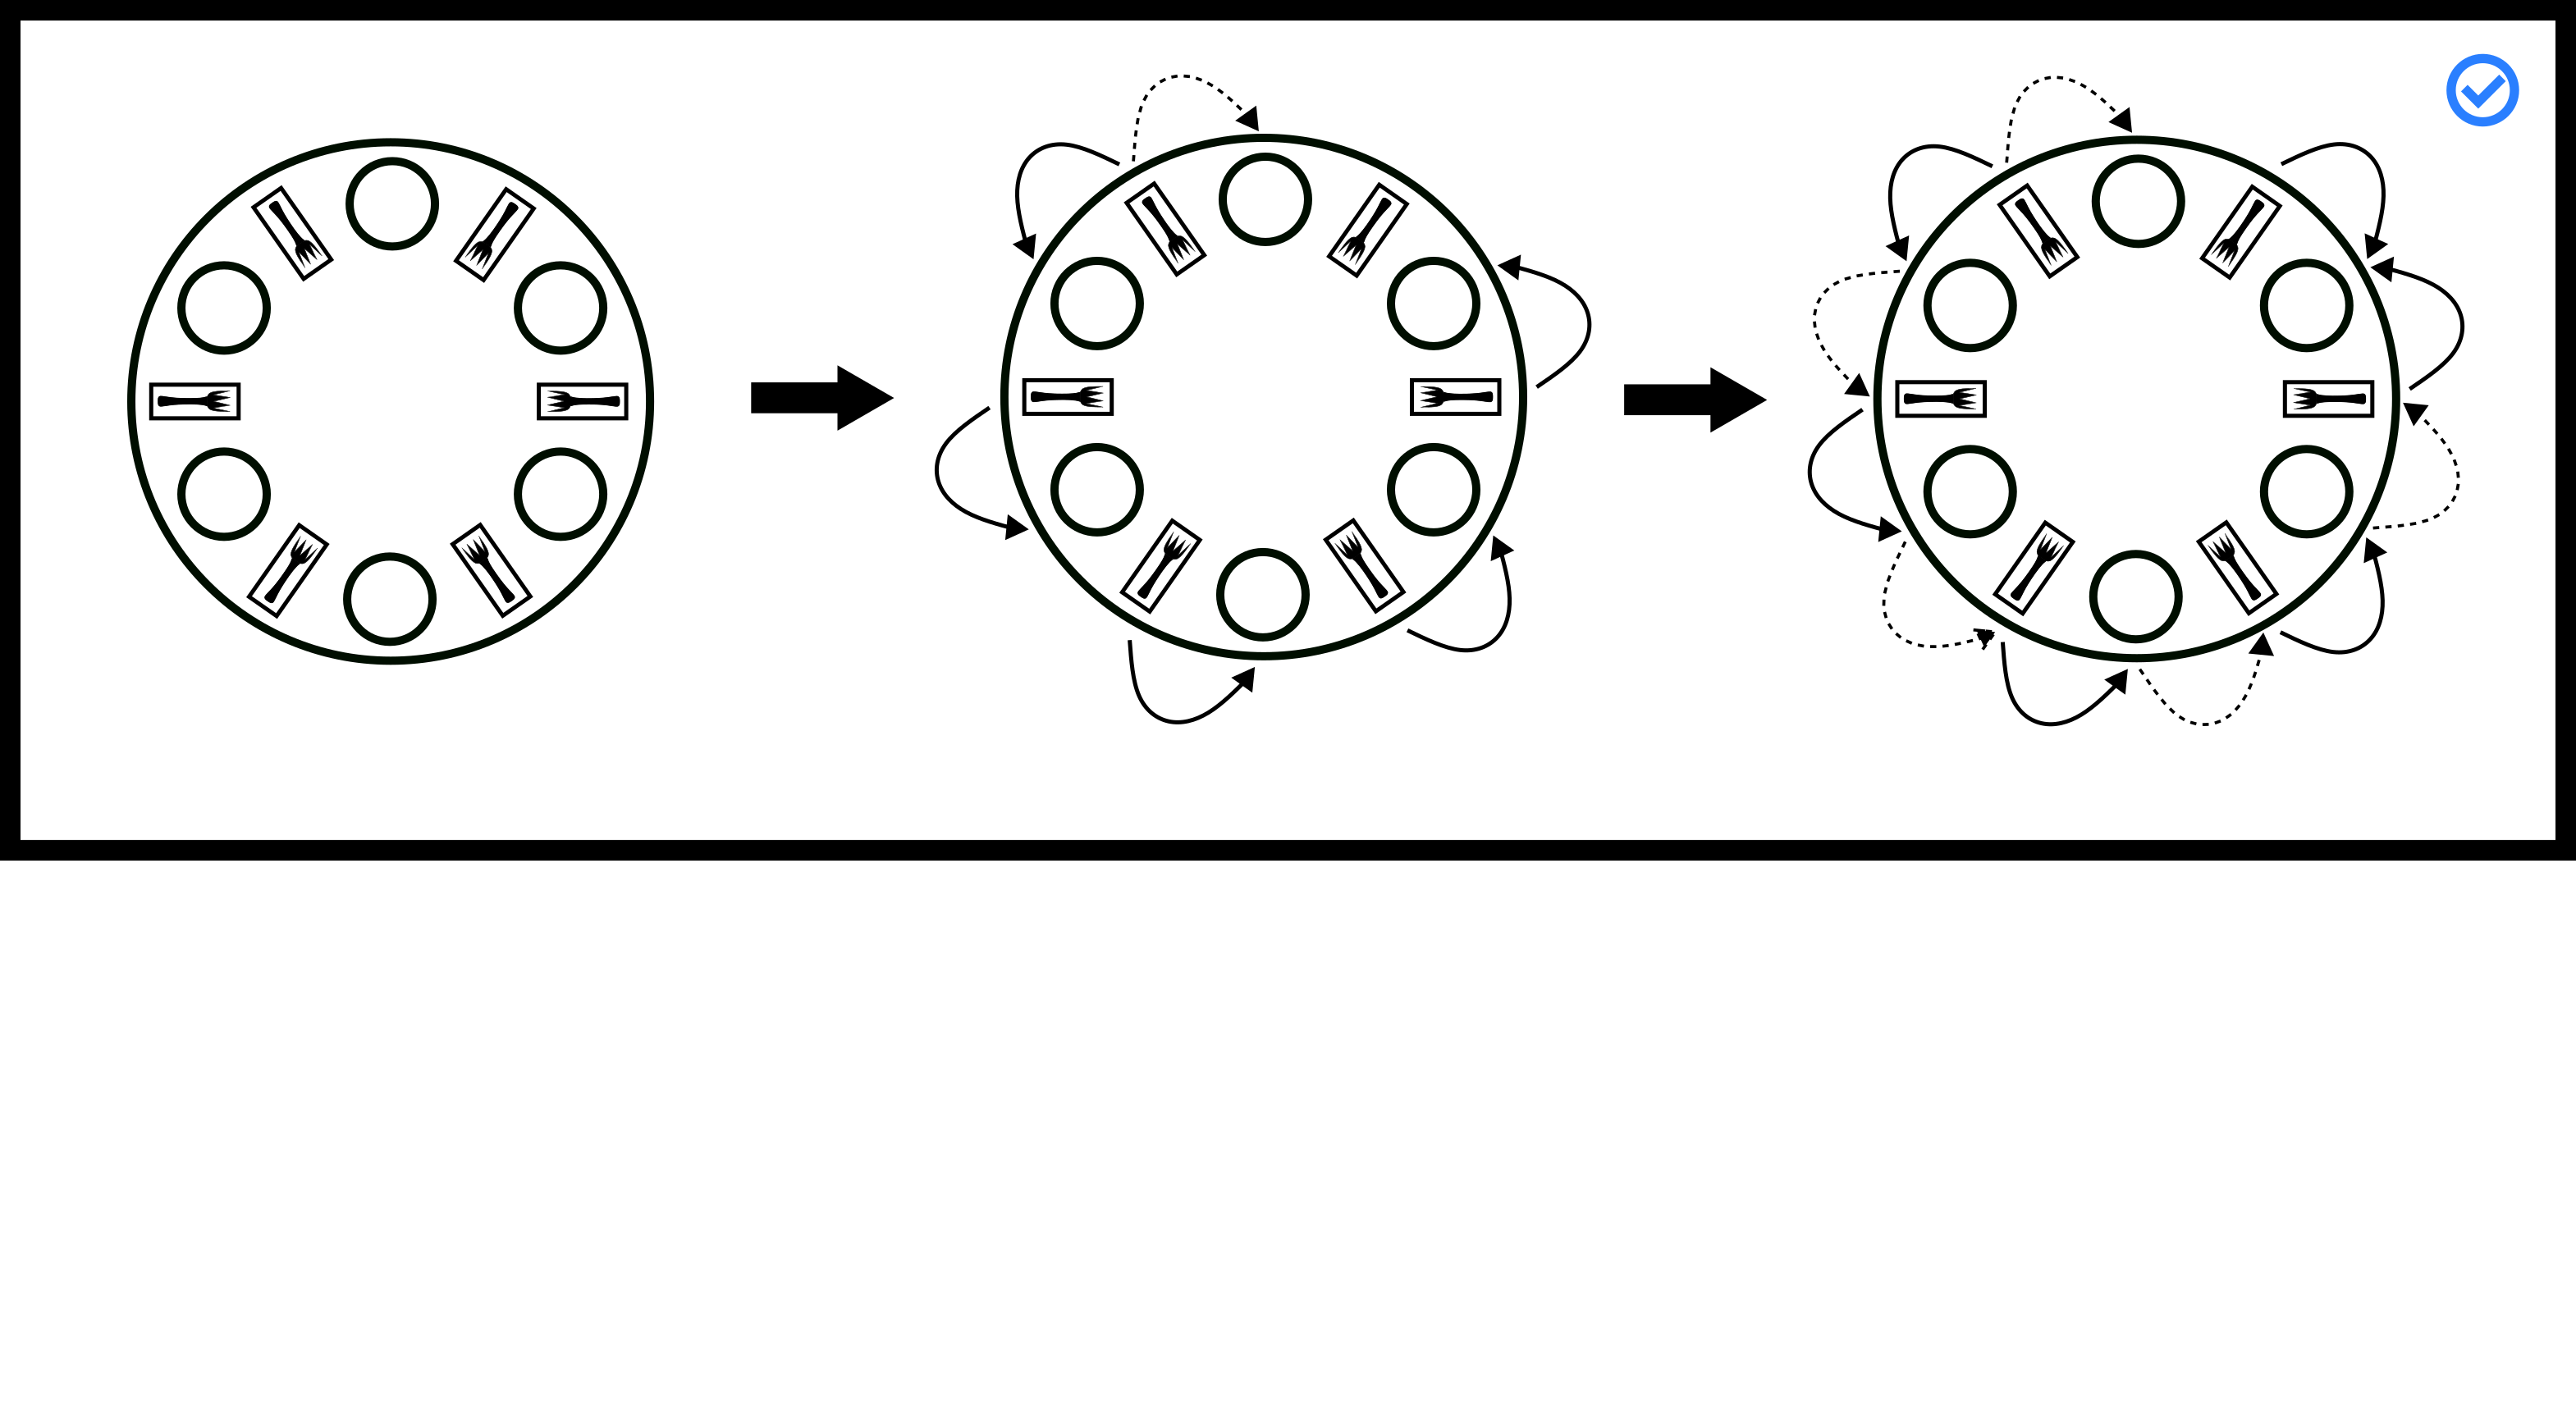
\includegraphics[width=.9\textwidth]{deadlock/drawings/dining_partial.png}
\caption{Stalling solution partial deadlock}
\end{figure}

\subsection{Extra: Clean/Dirty Forks (Chandy/Misra Solution)}

There are many more advanced solutions. One such solution is by Chandy and Misra \cite{Chandy:1984:DPP:1780.1804}. This is not a true solution to the dining philosophers problem because it has the requirement the philosophers can speak to each other. Basically though, it is a solution that ensures fairness. It in essence defines a series of rounds that a philosopher must eat in a given round before going to the next one.

We won't detail the proof here because it is a little more involved, but feel free to read at the citation.

\subsection{Advanced Solutions: Actor Model (other Message passing models)}

The actor model is another form of synchronization that doesn't have to do anything with negotiating locks or waiting. The idea is very simple. Each actor can either perform work, create more actors, send messages, or respond to messages. Any time an actor needs something from another actor, it sends a message. Most importantly, an actor is only responsible for one things.
If we were implementing a real world application, we may have an actor that handles the database, one that handles the incoming connections, one that services the connections, etc etc.
These actors would pass messages to each other like ``there is a new connection'' from the incoming connection actor to the servicing actor.
The servicing actor may send a data request message the database actor and a data response message comes back.

While this seems like the perfect solution there are drawbacks.
The first is the actual library of communication needs to be synchronized.
If you don't have a framework that does this already -- like the Message Passing Interface or MPI for High Performance Computing -- then the framework will have to be built and would most likely be as much work to build efficiently compared to direct synchronization.
In addition the messages now encounter additional overhead for serializing and deserializing or at the very least ordering.
And a final drawback is that an actor could take an arbitrary long time to respond to a message, spurring the need for shadow actors who service the same job.

As mentioned, there are frameworks like \href{https://en.wikipedia.org/wiki/Message\_Passing\_Interface}{Message passing interface} that is somewhat based on the actor model and allows distributed systems in high performance computing to work effectively, but your mileage my vary
You don't need to know \textit{any} of the specifics of the model, just the high level description given above.
If you want to read further on the model, feel free to glance over the wikipedia page listed below.
\href{https://en.wikipedia.org/wiki/Actor\_model}{Further reading on the actor model}

\section{Topics}

\begin{itemize}
  \item Coffman Conditions
  \item Resource Allocation Graphs
  \item Dining Philosophers
  \item Failed DP Solutions
  \item Livelocking DP Solutions
  \item Working DP Solutions: Benefits/Drawbacks
  \item \href{http://adit.io/posts/2013-05-11-The-Dining-Philosophers-Problem-With-Ron-Swanson.html}{Ron Swanson Deadlock}
\end{itemize}

\section{Questions}

\begin{itemize}
\item
  What are the Coffman Conditions?
\item
  What do each of the Coffman conditions mean? (e.g.~can you provide a definition of each one)
\item
  Give a real life example of breaking each Coffman condition in turn. A situation to consider: Painters, Paint, Paint Brushes etc. How would you assure that work would get done?
\item
  Be able to identify when Dining Philosophers code causes a deadlock (or not). For example, if you saw the following code snippet which Coffman condition is not satisfied?

\begin{lstlisting}[language=C]
// Get both locks or none
pthread_mutex_lock(a);
if(pthread_mutex_trylock( b )) { /* failure */
  pthread_mutex_unlock( a );
}
\end{lstlisting}
\item
  The following calls are made

\begin{lstlisting}[language=c]
// Thread 1
pthread_mutex_lock(m1) // success
pthread_mutex_lock(m2) // blocks

// Thread 2
pthread_mutex_lock(m2) // success
pthread_mutex_lock(m1) // blocks
\end{lstlisting}

  What happens and why? What happens if a third thread calls
  \keyword{pthread\_mutex\_lock(m1)} ?
\item
  How many processes are blocked? As usual assume that a process is able
  to complete if it is able to acquire all of the resources listed
  below.

  \begin{itemize}
  \tightlist
  \item
    P1 acquires R1
  \item
    P2 acquires R2
  \item
    P1 acquires R3
  \item
    P2 waits for R3
  \item
    P3 acquires R5
  \item
    P1 waits for R4
  \item
    P3 waits for R1
  \item
    P4 waits for R5
  \item
    P5 waits for R1
  \end{itemize}
\end{itemize}

Draw out the resource graph!

\bibliographystyle{plainnat}
\bibliography{deadlock/deadlock}

%\section{Thinking about scheduling.}\label{thinking-about-scheduling.}

\href{https://en.wikipedia.org/wiki/Scheduling_(computing)}{CPU
Scheduling} is the problem of efficiently selecting which process to run
on a system's CPU cores. In a busy system there will be more
ready-to-run processes than there are CPU cores, so the system kernel
must evaluate which processes should be scheduled to run on the CPU and
which processes should be placed in a ready queue to be executed later.

The additional complexity of multi-threaded and multiple CPU cores are
considered a distraction to this initial exposition so are ignored here.

Another gotcha for non-native speakers is the dual meanings of ``Time'':
The word ``Time'' can be used in both clock and elapsed duration
context. For example ``The arrival time of the first process was
9:00am.'' and, ``The running time of the algorithm is 3 seconds''.

\subsection{How is scheduling measured and which scheduler is
best?}\label{how-is-scheduling-measured-and-which-scheduler-is-best}

Scheduling affects the performance of the system, specifically the
\emph{latency} and \emph{throughput} of the system. The throughput might
be measured by a system value, for example the I/O throughput - the
number of bytes written per second, or number of small processes that
can complete per unit time, or using a higher level of abstraction for
example number of customer records processed per minute. The latency
might be measured by the response time (elapse time before a process can
start to send a response) or wait time or turnaround time (the elapsed
time to complete a task). Different schedulers offer different
optimization trade-offs that may or may not be appropriate to desired
use - there is no optimal scheduler for all possible environments and
goals. For example `shortest-job-first' will minimize total wait time
across all jobs but in interactive (UI) environments it would be
preferable to minimize response time (at the expense of some
throughput), while FCFS seems intuitively fair and easy to implement but
suffers from the Convoy Effect.

\subsection{What is arrival time?}\label{what-is-arrival-time}

The time at which a process first arrives at the ready queue, and is
ready to start executing. If a CPU is idle, the arrival time would also
be the starting time of execution.

\subsection{What is preemption?}\label{what-is-preemption}

Without preemption processes will run until they are unable to utilize
the CPU any further. For example the following conditions would remove a
process from the CPU and the CPU would be available to be scheduled for
other processes: The process terminates due to a signal, is blocked
waiting for concurrency primitive, or exits normally. Thus once a
process is scheduled it will continue even if another process with a
high priority (e.g.~shorter job) appears on the ready queue.

With preemption, the existing processes may be removed immediately if a
more preferable process is added to the ready queue. For example,
suppose at t=0 with a Shortest Job First scheduler there are two
processes (P1 P2) with 10 and 20 ms execution times. P1 is scheduled. P1
immediately creates a new process P3, with execution time of 5 ms, which
is added to the ready queue. Without preemption, P3 will run 10ms later
(after P1 has completed). With preemption, P1 will be immediately
evicted from the CPU and instead placed back in the ready queue, and P3
will be executed instead by the CPU.

\subsection{Which schedulers suffer from
starvation?}\label{which-schedulers-suffer-from-starvation}

Any scheduler that uses a form of prioritization can result in
starvation because earlier processes may never be scheduled to run
(assigned a CPU). For example with SJF, longer jobs may never be
scheduled if the system continues to have many short jobs to schedule.
It all depends on the
\href{https://en.wikipedia.org/wiki/Scheduling_(computing)\#Types_of_operating_system_schedulers}{type
of scheduler}.

\subsection{Why might a process (or thread) be placed on the ready
queue?}\label{why-might-a-process-or-thread-be-placed-on-the-ready-queue}

A process is placed on the ready queue when it is able to use a CPU.
Some examples include: * A process was blocked waiting for a
\texttt{read} from storage or socket to complete and data is now
available. * A new process has been created and is ready to start. * A
process thread was blocked on a synchronization primitive (condition
variable, semaphore, mutex lock) but is now able to continue. * A
process is blocked waiting for a system call to complete but a signal
has been delivered and the signal handler needs to run.

Similar examples can be generated when considering threads.

\section{Measures of Efficiency}\label{measures-of-efficiency}

\texttt{start\_time} is the wall-clock start time of the process (CPU
starts working on it) \texttt{end\_time} is the end wall-clock of the
process (CPU finishes the process) \texttt{run\_time} is the total
amount of CPU time required \texttt{arrival\_time} is the time the
process enters the scheduler (CPU may not start working on it)

\subsection{\texorpdfstring{What is `turnaround
time'?}{What is turnaround time?}}\label{what-is-turnaround-time}

The total time from when you the process arrives to when it ends.

\texttt{turnaround\_time\ =\ end\_time\ -\ arrival\_time}

\subsection{\texorpdfstring{What is `response
time'?}{What is response time?}}\label{what-is-response-time}

The total latency (time) that it takes from when the process arrives to
when the CPU actually starts working on it.

\texttt{response\_time\ =\ start\_time\ -\ arrival\_time}

\subsection{\texorpdfstring{What is `wait
time'?}{What is wait time?}}\label{what-is-wait-time}

Wait time is the \emph{total} wait time i.e.~the total time that a
process is on the ready queue. A common mistake is to believe it is only
the initial waiting time in the ready queue.

If a CPU intensive process with no I/O takes 7 minutes of CPU time to
complete but required 9 minutes of wall-clock time to complete we can
conclude that it was placed on the ready-queue for 2 minutes. For those
2 minutes the process was ready to run but had no CPU assigned. It does
not matter when the job was waiting, the wait time is 2 minutes.

\texttt{wait\_time\ \ =\ (end\_time\ -\ arrival\_time)\ -\ run\_time}

\subsection{What is the Convoy Effect?}\label{what-is-the-convoy-effect}

``The Convoy Effect is where I/O intensive processes are continually
backed up, waiting for CPU-intensive processes that hog the CPU. This
results in poor I/O performance, even for processes that have tiny CPU
needs.''

Suppose the CPU is currently assigned to a CPU intensive task and there
is a set of I/O intensive processes that are in the ready queue. These
processes require just a tiny amount of CPU time but they are unable to
proceed because they are waiting for the CPU-intensive task to be
removed from the processor. These processes are starved until the the
CPU bound process releases the CPU. But the CPU will rarely be released
(for example in the case of a FCFS scheduler, we must wait until the
processes is blocked due to an I/O request). The I/O intensive processes
can now finally satisfy their CPU needs, which they can do quickly
because their CPU needs are small and the CPU is assigned back to the
CPU-intensive process again. Thus the I/O performance of the whole
system suffers through an indirect effect of starvation of CPU needs of
all processes.

This effect is usually discussed in the context of FCFS scheduler,
however a round robin scheduler can also exhibit the Convoy effect for
long time-quanta.

\subsection{Linux Scheduling}\label{linux-scheduling}

As of February 2016, Linux by default uses the \emph{Completely Fair
Scheduler} for CPU scheduling and the Budget Fair Scheduling ``BFQ'' for
I/O scheduling. Appropriate scheduling can have a significant impact on
throughput and latency. Latency is particularly important for
interactive and soft-real time applications such as audio and video
streaming. See the discussion and comparative benchmarks
\href{https://lkml.org/lkml/2014/5/27/314}{here} for more information.

Here is how the CFS schedules

\begin{itemize}
\tightlist
\item
  The CPU creates a Red-Black tree with the processes virtual runtime
  (runtime / nice\_value) and sleeper fairness (if the process is
  waiting on something give it the CPU when it is done waiting).
\item
  (Nice values are the kernel's way of giving priority to certain
  processes, the lower nice value the higher priority)
\item
  The kernel chooses the lowest one based on this metric and schedules
  that process to run next, taking it off the queue. Since the red-black
  tree is self balancing this operation is guaranteed \(O(log(n))\)
  (selecting the min process is the same runtime)
\end{itemize}

Although it is called the Fair Scheduler there are a fair bit of
problems.

\begin{itemize}
\tightlist
\item
  Groups of processes that are scheduled may have imbalanced loads so
  the scheduler roughly distributes the load. When another CPU gets free
  it can only look at the average load of a group schedule not the
  individual cores. So the free CPU may not take the work from a CPU
  that is burning so long as the average is fine.
\item
  If a group of processes is running on non-adjacent cores then there is
  a bug. If the two cores are more than a hop away, the load balancing
  algorithm won't even consider that core. Meaning if a CPU is free and
  a CPU that is doing more work is more than a hop away, it won't take
  the work (may have been patched).
\item
  After a thread goes to sleep on a subset of cores, when it wakes up it
  can only be scheduled on the cores that it was sleeping on. If those
  cores are now busy, the thread will have to wait on them, wasting
  opportunities to use other idle cores.
\item
  To read more on the problems of the Fair Scheduler, read
  \href{https://blog.acolyer.org/2016/04/26/the-linux-scheduler-a-decade-of-wasted-cores}{here}.
\end{itemize}

\section{What are some well known scheduling
algorithms?}\label{what-are-some-well-known-scheduling-algorithms}

For all the examples,

Process 1: Runtime 1000ms

Process 2: Runtime 2000ms

Process 3: Runtime 3000ms

Process 4: Runtime 4000ms

Process 5: Runtime 5000ms

\section{Shortest Job First (SJF)}\label{shortest-job-first-sjf}

\begin{figure}[htbp]
\centering
\includegraphics{http://i.imgur.com/jGLvjqT.png}
\caption{}
\end{figure}

\begin{itemize}
\tightlist
\item
  P1 Arrival: 0ms
\item
  P2 Arrival: 0ms
\item
  P3 Arrival: 0ms
\item
  P4 Arrival: 0ms
\item
  P5 Arrival: 0ms
\end{itemize}

The processes all arrive at the start and the scheduler schedules the
job with the shortest total CPU time. The glaring problem is that this
scheduler needs to know how long this program will run over time before
it ran the program.

Technical Note: A realistic SJF implementation would not use the total
execution time of the process but the burst time (the total CPU time
including future computational execution before the process will no
longer be ready to run). The expected burst time can be estimated by
using an exponentially decaying weighted rolling average based on the
previous burst time but for this exposition we will simplify this
discussion to use the total running time of the process as a proxy for
the burst time.

\textbf{Advantages} * Shorter jobs tend to get run first

\textbf{Disadvantages} * Needs algorithm to be omniscient

\section{Preemptive Shortest Job First
(PSJF)}\label{preemptive-shortest-job-first-psjf}

Preemptive shortest job first is like shortest job first but if a new
job comes in with a shorter runtime than the total runtime of the
current job, it is run instead. (If it is equal like our example our
algorithm can choose). The scheduler uses the \emph{total} runtime of
the process. If you want the shortest \emph{remaining} time left, that
is a variant of PSJF called Shortest Remaining Time First (SRTF).

\begin{figure}[htbp]
\centering
\includegraphics{http://i.imgur.com/QvoX7Ia.png}
\caption{}
\end{figure}

\begin{itemize}
\tightlist
\item
  P2 at 0ms
\item
  P1 at 1000ms
\item
  P5 at 3000ms
\item
  P4 at 4000ms
\item
  P3 at 5000ms
\end{itemize}

Here's what our algorithm does. It runs P2 because it is the only thing
to run. Then P1 comes in at 1000ms, P2 runs for 2000ms, so our scheduler
preemptively stops P2, and let's P1 run all the way through (this is
completely up to the algorithm because the times are equal). Then, P5
Comes in -- since there are no processes running, the scheduler will run
process 5. P4 comes in, and since the runtimes are equal P5, the
scheduler stops P5 and runs P4. Finally P3 comes in, preempts P4, and
runs to completion. Then P4 runs, then P5 runs.

\textbf{Advantages} * Ensures shorter jobs get run first

\textbf{Disadvantages} * Need to know the runtime again

\section{First Come First Served
(FCFS)}\label{first-come-first-served-fcfs}

\begin{figure}[htbp]
\centering
\includegraphics{http://i.imgur.com/lcMpUZz.png}
\caption{}
\end{figure}

\begin{itemize}
\tightlist
\item
  P2 at 0ms
\item
  P1 at 1000ms
\item
  P5 at 3000ms
\item
  P4 at 4000ms
\item
  P3 at 5000ms
\end{itemize}

Processes are scheduled in the order of arrival. One advantage of FCFS
is that scheduling algorithm is simple: the ready queue is a just a FIFO
(first in first out) queue. FCFS suffers from the Convoy effect.

Here P2 Arrives, then P1 arrives, then P5, then P4, then P3. You can see
the convoy effect for P5.

\textbf{Advantages} * Simple implementation

\textbf{Disadvantages} * Long running processes could block all other
processes

\section{Round Robin (RR)}\label{round-robin-rr}

Processes are scheduled in order of their arrival in the ready queue.
However after a small time step a running process will be forcibly
removed from the running state and placed back on the ready queue. This
ensures that a long-running process can not starve all other processes
from running. The maximum amount of time that a process can execute
before being returned to the ready queue is called the time quanta. In
the limit of large time quanta (where the time quanta is longer than the
running time of all processes) round robin will be equivalent to FCFS.

\begin{figure}[htbp]
\centering
\includegraphics{http://i.imgur.com/AlBYi0Y.png}
\caption{}
\end{figure}

\begin{itemize}
\tightlist
\item
  P1 Arrival: 0ms
\item
  P2 Arrival: 0ms
\item
  P3 Arrival: 0ms
\item
  P4 Arrival: 0ms
\item
  P5 Arrival: 0ms
\end{itemize}

Quantum = 1000ms

Here all processes arrive at the same time. P1 is run for 1 quantum and
is finished. P2 for one quantum; then, it is stopped for P3. After all
other processes run for a quantum we cycle back to P2 until all the
processes are finished.

\textbf{Advantages} * Ensures some notion of fairness

\textbf{Disadvantages} * Large number of processes = Lots of switching

\section{Priority}\label{priority}

Processes are scheduled in the order of priority value. For example, a
navigation process might be more important to execute than a logging
process.

\section{Topics}\label{topics}

\begin{itemize}
\tightlist
\item
  Virtual Memory
\item
  Page Table
\item
  MMU/TLB
\item
  Address Translation
\item
  Page Faults
\item
  Frames/Pages
\item
  Single level vs multi level page table
\item
  Calculating offsets for multi-level page table
\item
  Pipes
\item
  Pipe read write ends
\item
  Writing to a zero reader pipe
\item
  Reading from a zero writer pipe
\item
  Named pipe and Unnamed Pipes
\item
  Buffer Size/Atomicity
\item
  Scheduling Algorithms
\item
  Measures of Efficiency
\end{itemize}

\section{Questions}\label{questions}

\begin{itemize}
\tightlist
\item
  What is virtual memory?
\item
  What are the following and what is their purpose?

  \begin{itemize}
  \tightlist
  \item
    Translation Lookaside Buffer
  \item
    Physical Address
  \item
    Memory Management Unit. Multilevel page table. Frame number. Page
    number and page offset.
  \item
    The dirty bit
  \item
    The NX Bit
  \end{itemize}
\item
  What is a page table? How about a physical frame? Does a page always
  need to point to a physical frame?
\item
  What is a page fault? What are the types? When does it result in a
  segfault?
\item
  What are the advantages to a single level page table? Disadvantages?
  How about a multi leveled table?
\item
  What does a multi leveled table look like in memory?
\item
  How do you determine how many bits are used in the page offset?
\item
  Given a 64 bit address space, 4kb pages and frames, and a 3 level page
  table, how many bits is the Virtual page number 1, VPN2, VPN3 and the
  offset?
\item
  What is a pipe? How do I create a pipe?
\item
  When is SIGPIPE delivered to a process?
\item
  Under what conditions will calling read() on a pipe block? Under what
  conditions will read() immediately return 0
\item
  What is the difference between a named pipe and an unnamed pipe?
\item
  Is a pipe thread safe?
\item
  Write a function that uses fseek and ftell to replace the middle
  character of a file with an `X'
\item
  Write a function that create a pipe and uses write to send 5 bytes,
  ``HELLO'' to the pipe. Return the read file descriptor of the pipe.
\item
  What happens when you mmap a file?
\item
  Why is getting the file size with ftell not recommended? How should
  you do it instead?
\item
  What is scheduling?
\item
  What is turnaround time? Response Time? Wait time?
\item
  What is the convoy effect?
\item
  Which algorithms have the best turnaround/response/wait time on
  average
\end{itemize}

%\chapter{Interprocess Communication}

\todo{Epigraph}

In very simple embedded systems and early computers, processes directly access memory i.e. ``Address 1234'' corresponds to a particular byte stored in a particular part of physical memory. For example the IBM 709 had to read and write directly to a tape with no level of abstraction \cite[P. 65]{ibm709}. Even in systems after that, it was hard to adopt virtual memory because virtual memory required the whole fetch cycle to be altered through hardware -- a change many manufacturers still thought was expensive. In the PDP-10, a workaround was used by using different registers for each process and then virtual memory was added later. In modern systems, this is no longer the case. Instead each process is isolated, and there is a translation process between the address of a particular CPU instruction or piece of data of a process and the actual byte of physical memory (``RAM''). Memory addresses no longer map to physical addresses; the process runs inside virtual memory. Virtual memory not only keeps processes safe (because one process cannot directly read or modify another process's memory) it also allows the system to efficiently allocate and re-allocate portions of memory to different processes. The modern process of translating memory is as follows.

\begin{enumerate}
\item A process makes a memory request
\item The circuit first checks the Translation Lookaside Buffer (TLB) if the address page is cached into memory. It skips to the reading from/writing to phase if found otherwise the request goes to the MMU.
\item The Memory Management Unit (MMU) performs the address translation. If the translation succeeds (more on that later), the page get pulled from RAM -- conceptually the entire page isn't loaded up. The result is cached in the TLB. 
\item The CPU performs the operation by either reading from the physical address or writing to the address.
\end{enumerate}

\section{MMU and Translating Addresses}

The Memory Management Unit is part of the CPU, and it converts a virtual memory address into a physical address. There is a sort of pseudocode associated with the MMU.

\begin{enumerate}
\item Receive address
\item Try to translate address according to the programmed scheme
\item If the translation fails, report an invalid address
\item Otherwise,
	\begin{enumerate}
	\item If the page exists in memory, check if the process has permissions
		to perform the operation on the page meaning the process has access
		to the page, and it is reading from the page/writing to a page
		that is not marked as read only.
		\begin{enumerate}
		\item If so then provide the address, cache the results in the TLB
		\item Otherwise trigger a hardware interrupt. The kernel 
			will most likely send a SIGSEGV or a Segmentation Violation.
		\end{enumerate}
	\item If the page doesn't exist in memory, generate an Interrupt.
		\begin{enumerate}
		\item The kernel could realize that this page could either be not
			allocated or on disk. If it fits the mapping, allocate the page
			and try the operation again.
		\item Otherwise, this is an invalid access and the kernel will most
			likely send a SIGSEGV to the process.
		\end{enumerate}
	\end{enumerate}
\end{enumerate}

Imagine you had a 32 bit machine, meaning pointers are 32 bits. They can address $2^{32}$ different locations or 4GB of memory where one address is one byte. Imagine we had a large table - here's the clever part - stored in memory! For every possible address (all 4 billion of them) we will store the `real' i.e. ~physical address. Each physical address will need 4 bytes (to hold the 32 bits). This scheme would require 16 billion bytes to store all of entries. Oops - our lookup scheme would consume all of the memory that we could possibly buy for our 4GB machine. We need to do better than this. Our lookup table better be smaller than the memory we have otherwise we will have no space left for our actual programs and operating system data. The solution is to chunk memory into small regions called `pages' and `frames' and use a lookup table for each page.

A \textbf{page} is a block of virtual memory. A typical block size on Linux operating system is 4KB or $2^{12}$ addresses, though you can find examples of larger blocks. So rather than talking about individual bytes we can talk about blocks of 4KBs, each block is called a page. We can also number our pages (``Page 0'' ``Page 1'' etc). Let's do a sample calculation of how many pages are there assume page size of 4KB.

\begin{shaded*}
For a 32 bit machine, $2^{32}$ address / $2^{12}$ (address/page) = $2^{20}$ pages.

For a 64 bit machine, $2^{64}$ / $2^{12}$ = $2^{52}$, which is roughly $10^{15}$ pages.
\end{shaded*}

\subsection{Terminology}

A \textbf{frame} (or sometimes called a `page frame') is a block of \emph{physical memory} or RAM (=Random Access Memory). This kind of memory is occasionally called `primary storage' in contrast with lower, secondary storage such as spinning disks that have lower access times. A frame is the same number of bytes as a virtual page. If a 32 bit machine has $2^{32} B$ of RAM, then there will be the same number of them in the addressable space of the machine. It's unlikely that a 64 bit machine will ever have $2^{64}$ bytes of RAM.

A \textbf{page table} is a mapping between a page to the frame. For example Page 1 might be mapped to frame 45, page 2 mapped to frame 30. Other frames might be currently unused or assigned to other running processes, or used internally by the operating system.

A simple page table could be imagined as an array.
\begin{lstlisting}[language=C]
int frame_num = table[page_num]; 
\end{lstlisting}

For a 32 bit machine with 4KB pages, each entry needs to hold a frame number - i.e.~20 bits because we calculated there are $2^{20}$ frames. That's 2.5 bytes per entry! In practice, we'll round that up to 4 bytes per entry and find a use for those spare bits. With 4 bytes per entry x $2^{20}$ entries = 4 MB of physical memory are required to hold the page table 
For a 64 bit machine with 4KB pages, each entry needs 52 bits. Let's round up to 64 bits (8 bytes) per entry. With $2^{52}$ entries thats $2^{55}$ bytes (roughly 40 peta bytes\ldots{}) Oops our page table is too large 
In 64 bit architectures memory addresses are sparse, so we need a mechanism to reduce the page table size, given that most of the entries will never be used.

\begin{wrapfig}
% 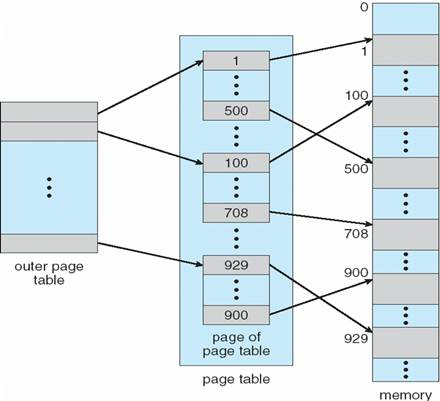
\includegraphics{ipc/images/page_table1.jpg}
\end{wrapfig}

An \textbf{offset} take a particular page and looks up a byte by adding it to the start of the page. Remember our page table maps pages to frames, but each page is a block of contiguous addresses. How do we calculate which particular byte to use inside a particular frame? The solution is to re-use the lowest bits of the virtual memory address directly. For example, suppose our process is reading the following address- \keyword{VirtualAddress = 11110000111100001111000010101010 (binary)}

On a machine with page size 256 Bytes, then the lowest 8 bits (10101010) will be used as the offset. The remaining upper bits will be the page number (111100001111000011110000).

\subsection{Multi-level page tables}\label{multi-level-page-tables}
 Multi-level pages are one solution to the page table size issue for 64 bit architectures. We'll look at the simplest implementation - a two level page table. Each table is a list of pointers that point to the next level of tables, not all sub-tables need to exist. An example, two level page table for a 32 bit architecture is shown below-

\begin{verbatim}
VirtualAddress = 11110000111111110000000010101010 (binary)
                 |-Index1-||        ||          | 10 bit Directory index
                           |-Index2-||          | 10 bit Sub-table index
                                     |--offset--| 12 bit offset (passed directly to RAM)
\end{verbatim}

 In the above scheme, determining the frame number requires two memory reads: The topmost 10 bits are used in a directory of page tables. If 2 bytes are used for each entry, we only need 2KB to store this entire directory. Each subtable will point to physical frames (i.e.~required 4 bytes to store the 20 bits). However, for processes with only tiny memory needs, we only need to specify entries for low memory address (for the heap and program code) and high memory addresses (for the stack). Each subtable is 1024 entries x 4 bytes i.e.~4KB for each subtable.

 Thus the total memory overhead for our multi-level page table has shrunk from 4MB (for the single level implementation) to 3 frames of memory (12KB) ! Here's why: We need at least one frame for the high level directory and two frames for just two sub-tables. One sub-table is necessary for the low addresses (program code, constants and possibly a tiny heap), the other sub-table is for higher addresses used by the environment and stack. In practice, real programs will likely need more sub-table entries, as each subtable can only reference 1024*4KB = 4MB of address space but the main point still stands - we have significantly reduced the memory overhead required to perform page table look ups.

\subsection{Page Table Disadvantages}
 Yes - Significantly ! (But thanks to clever hardware, usually no\ldots{}) Compared to reading or writing memory directly. For a single page table, our machine is now twice as slow! (Two memory accesses are required) For a two-level page table, memory access is now three times as slow. (Three memory accesses are required)

 To overcome this overhead, the MMU includes an associative cache of recently-used virtual-page-to-frame lookups. This cache is called the TLB (``translation lookaside buffer''). Everytime a virtual address needs to be translated into a physical memory location, the TLB is queried in parallel to the page table. For most memory accesses of most programs, there is a significant chance that the TLB has cached the results. However if a program does not have good cache coherence (for example is reading from random memory locations of many different pages) then the TLB will not have the result cache and now the MMU must use the much slower page table to determine the physical frame.

\begin{wrapfig}
% 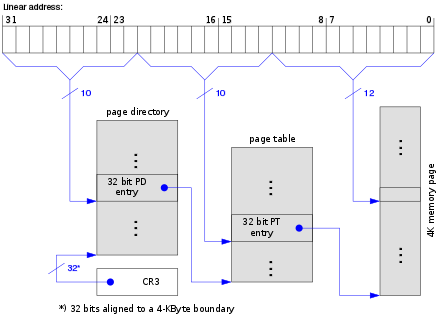
\includegraphics{ipc/images/440px-X86_Paging_4K.png}
\end{wrapfig}

This may be how one splits up a multi level page table.

\section{Advanced Frames and Page Protections}\label{advanced-frames-and-page-protections}

Frames be shared between processes! In addition to storing the frame number, the page table can be used to store whether a process can write or only read a particular frame. Read only frames can then be safely shared between multiple processes. For example, the C-library instruction code can be shared between all processes that dynamically load the code into the process memory. Each process can only read that memory. Meaning that if you try to write to a read-only page in memory you will get a \keyword{SEGFAULT}. That is why sometimes memory accesses segfault and sometimes they don't, it all depends on if your hardware says that you can access.

In addition, processes can share a page with a child process using the \keyword{mmap} system call. \keyword{mmap} is an interesting call because instead of tying each virtual address to a physical frame, it ties it to something else. That something else can be a file, a GPU unit, or any other memory mapped operation that you can think of! Writing to the memory address may write through to the device or the write may be paused by the operating system but this is a very powerful abstraction because often the operating system is able to perform optimizations (multiple processes memory mapping the same file can have the kernel create one mapping). In addition, it is common to store at least read-only, modification and execution information.

\subsubsection{Read-only bit}
The read-only bit marks the page as read-only. Attempts to write to the page will cause a page fault. The page fault will then be handled by the Kernel. Two examples of the read-only page include sharing the c runtime library between multiple processes (for security you wouldn't want to allow one process to modify the library); and Copy-On-Write where the cost of duplicating a page can be delayed until the first write occurs.

\subsubsection{Dirty bit}

\href{http://en.wikipedia.org/wiki/Page\_table\#Page\_table\_data}{Page Table} The dirty bit allows for a performance optimization. A page on disk that is paged in to physical memory, then read from, and subsequently paged out again does not need to be written back to disk, since the page hasn't changed. However, if the page was written to after it's paged in, its dirty bit will be set, indicating that the page must be written back to the backing store. This strategy requires that the backing store retain a copy of the page after it is paged in to memory. When a dirty bit is not used, the backing store need only be as large as the instantaneous total size of all paged-out pages at any moment. When a dirty bit is used, at all times some pages will exist in both physical memory and the backing store.

\subsubsection{Execution bit}\label{execution-bit}
The execution bit defines whether bytes in a page can be executed as CPU instructions. By disabling a page, it prevents code that is maliciously stored in the process memory (e.g.~by stack overflow) from being easily executed. (further reading: \href{http://en.wikipedia.org/wiki/NX\_bit\#Hardware\_background}{background})

\subsection{Page Faults}

 A page fault is when a running program tries to access some virtual memory in its address space that is not mapped to physical memory. Page faults will also occur in other situations. There are three types of Page Faults

\begin{enumerate}
 \item \textbf{Minor} If there is no mapping yet for the page, but it is a valid address. This could be memory asked for by \keyword{sbrk(2)} but not written to yet meaning that the operating system can wait for the first write before allocating space. The OS simply makes the page, loads it into memory, and moves on.

 \item \textbf{Major} If the mapping to the page is not in memory but on disk. What this will do is swap the page into memory and swap another page out. If this happens frequently enough, your program is said to \emph{thrash} the MMU.

 \item \textbf{Invalid} When you try to write to a non-writable memory address or read to a non-readable memory address. The MMU generates an invalid fault and the OS will usually generate a \keyword{SIGSEGV} meaning segmentation violation meaning that you wrote outside the segment that you could write to.
\end{enumerate}

\section{Pipes}

Inter process communication is any way for one process to talk to another process. You've already seen one form of this virtual memory! A piece of virtual memory can be shared between parent and child, leading to communication. You may want to wrap that memory in \keyword{pthread\_mutexattr\_setpshared(\&attrmutex,\ PTHREAD\_PROCESS\_SHARED);} mutex (or a process wide mutex) to prevent race conditions. There are more standard ways of IPC, like pipes! Consider if you type the following into your terminal.

\begin{verbatim}
$ ls -1 | cut -d'.' -f1 | uniq | sort | tee dir_contents
\end{verbatim}

What does the following code do? Well it \keyword{ls}'s the current directory (the -1 means that it outputs one entry per line). The \keyword{cut} command then takes everything before the first period. Uniq makes sure all the lines are uniq, sort sorts them and tee outputs to a file. The important part is that bash creates \textbf{5 separate processes} and connects their standard outs/stdins with pipes the trail lookssomething like this.

\begin{verbatim}
(0) ls (1)------>(0) cut (1)------->(0) uniq (1)------>(0) sort (1)------>(0) tee (1)
\end{verbatim}

The numbers in the pipes are the file descriptors for each process and the arrow represents the redirect or where the output of the pipe is going. A POSIX pipe is almost like its real counterpart - you can stuff bytes down one end and they will appear at the other end in the same order. Unlike real pipes however, the flow is always in the same direction, one file descriptor is used for reading and the other for writing. The \keyword{pipe} system call is used to create a pipe. These file descriptors can be used with \keyword{read} and with \keyword{write}. A common method of using pipes is to create the pipe before forking in order to communicate with a child process

\begin{lstlisting}[language=C]
int filedes[2];
pipe (filedes);
pid_t child = fork();
if (child > 0) { /* I must be the parent */
    char buffer[80];
    int bytesread = read(filedes[0], buffer, sizeof(buffer));
    // do something with the bytes read    
} else {
	write(filedes[1], "done", 4);
}
\end{lstlisting}

One can use pipes inside of the same process, but there tends to be no added benefit. Here's an example program that sends a message to itself:

\begin{lstlisting}[language=C]
#include <unistd.h>
#include <stdlib.h>
#include <stdio.h>

int main() {
    int fh[2];
    pipe(fh);
    FILE *reader = fdopen(fh[0], "r");
    FILE *writer = fdopen(fh[1], "w");
    // Hurrah now I can use printf rather than using low-level read() write()
    printf("Writing...\n");
    fprintf(writer,"%d %d %d\n", 10, 20, 30);
    fflush(writer);
    
    printf("Reading...\n");
    int results[3];
    int ok = fscanf(reader,"%d %d %d", results, results + 1, results + 2);
    printf("%d values parsed: %d %d %d\n", ok, results[0], results[1], results[2]);
    
    return 0;
}
\end{lstlisting}

The problem with using a pipe in this fashion is that writing to a pipe can block meaning the pipe only has a limited buffering capacity. If the pipe is full the writing process will block! The maximum size of the buffer is system dependent; typical values from 4KB upto 128KB.

\begin{lstlisting}[language=C]
int main() {
    int fh[2];
    pipe(fh);
    int b = 0;
    #define MESG "..............................."
    while(1) {
        printf("%d\n",b);
        write(fh[1], MESG, sizeof(MESG))
        b+=sizeof(MESG);
    }
    return 0;
}
\end{lstlisting}

\subsection{Pipe Gotchas}\label{pipe-gotchas}

Here's a complete example that doesn't work! The child reads one byte at a time from the pipe and prints it out - but we never see the message! Can you see why?

\begin{lstlisting}[language=C]
#include <stdio.h>
#include <stdlib.h>
#include <unistd.h>
#include <signal.h>

int main() {
    int fd[2];
    pipe(fd);
    //You must read from fd[0] and write from fd[1]
    printf("Reading from %d, writing to %d\n", fd[0], fd[1]);

    pid_t p = fork();
    if (p > 0) {
        /* I have a child therefore I am the parent*/
        write(fd[1],"Hi Child!",9);

        /*don't forget your child*/
        wait(NULL);
    } else {
        char buf;
        int bytesread;
        // read one byte at a time.
        while ((bytesread = read(fd[0], &buf, 1)) > 0) {
            putchar(buf);
        }
    }
    return 0;
}
\end{lstlisting}

The parent sends the bytes \keyword{H,i,(space),C...!} into the pipe (this may block if the pipe is full). The child starts reading the pipe one byte at a time. In the above case, the child process will read and print each character. However it never leaves the while loop! When there are no characters left to read it simply blocks and waits for more 

The call \keyword{putchar} writes the characters out but we never flush the \keyword{stdout} buffer. i.e.~We have transferred the message from one process to another but it has not yet been printed. To see the message we could flush the buffer e.g. \keyword{fflush(stdout)} (or \keyword{printf("\textbackslash{}n")} if the output is going to a terminal). A better solution would also exit the loop by checking for an end-of-message marker,

\begin{lstlisting}[language=C]
        while ((bytesread = read(fd[0], &buf, 1)) > 0) {
            putchar(buf);
            if (buf == '!') break; /* End of message */
        }
\end{lstlisting}

Processes receive the signal SIGPIPE when no process is listening! From
the pipe(2) man page -

\begin{lstlisting}[language=C]
If all file descriptors referring to the read end of a pipe have been closed,
 then a write(2) will cause a SIGPIPE signal to be generated for the calling process. 
\end{lstlisting}

Tip: Notice only the writer (not a reader) can use this signal. To
inform the reader that a writer is closing their end of the pipe, you
could write your own special byte (e.g.~0xff) or a message (
\keyword{"Bye!"})

Here's an example of catching this signal that does not work! Can you
see why?

\begin{lstlisting}[language=C]
#include <stdio.h>
#include <stdio.h>
#include <unistd.h>
#include <signal.h>

void no_one_listening(int signal) {
    write(1, "No one is listening!\n", 21);
}

int main() {
    signal(SIGPIPE, no_one_listening);
    int filedes[2];
    
    pipe(filedes);
    pid_t child = fork();
    if (child > 0) { 
        /* I must be the parent. Close the listening end of the pipe */
        /* I'm not listening anymore!*/
        close(filedes[0]);
    } else {
        /* Child writes messages to the pipe */
        write(filedes[1], "One", 3);
        sleep(2);
        // Will this write generate SIGPIPE ?
        write(filedes[1], "Two", 3);
        write(1, "Done\n", 5);
    }
    return 0;
}
\end{lstlisting}

The mistake in above code is that there is still a reader for the pipe! The child still has the pipe's first file descriptor open and remember the specification? All readers must be closed 

When forking, \emph{It is common practice} to close the unnecessary (unused) end of each pipe in the child and parent process. For example the parent might close the reading end and the child might close the writing end (and vice versa if you have two pipes)

\subsection{Why is my pipe hanging?}\label{why-is-my-pipe-hanging}

Reads and writes hang on Named Pipes until there is at least one reader and one writer, take this

\begin{lstlisting}[language=C]
1$ mkfifo fifo
1$ echo Hello > fifo
# This will hang until I do this on another terminal or another process
2$ cat fifo
Hello
\end{lstlisting}

Any \keyword{open} is called on a named pipe the kernel blocks until another process calls the opposite open. Meaning, echo calls \keyword{open(..,\ O\_RDONLY)} but that blocks until cat calls \keyword{open(..,\ O\_WRONLY)}, then the programs are allowed to continue.

\subsection{Race condition with named pipes}

What is wrong with the following program?

\begin{lstlisting}[language=C]
//Program 1

int main(){
    int fd = open("fifo", O_RDWR | O_TRUNC);
    write(fd, "Hello!", 6);
    close(fd);
    return 0;
}

//Program 2
int main() {
    char buffer[7];
    int fd = open("fifo", O_RDONLY);
    read(fd, buffer, 6);
    buffer[6] = '\0';
    printf("%s\n", buffer);
    return 0;
}
\end{lstlisting}

This may never print hello because of a race condition. Since you opened the pipe in the first process under both permissions, open won't wait for a reader because you told the operating system that you are a reader! Sometimes it looks like it works because the execution of the code looks something like this.

\begin{enumerate}
\item Process 1: open(O\_RDWR) \& write()
\item Process 2: open(O\_RDONLY) \& read()
\item Process 1: close() \& exit()
\item Process 2: print() \& exit()
\end{enumerate}

\begin{enumerate}
\item Process 1: open(O\_RDWR) \& write()
\item Process 1: close() \& exit()
\item Process 2: open(O\_RDONLY) (Blocks indefinitely) 
\end{enumerate}

\subsection{What is filling up the pipe? What happens when the pipe
becomes
full?}\label{what-is-filling-up-the-pipe-what-happens-when-the-pipe-becomes-full}
 A pipe gets filled up when the writer writes too much to the pipe without the reader reading any of it. When the pipes become full, all writes fail until a read occurs. Even then, a write may partial fail if the pipe has a little bit of space left but not enough for the entire message 

 To avoid this, usually two things are done. Either increase the size of the pipe. Or more commonly, fix your program design so that the pipe is constantly being read from.

\subsection{Are pipes process safe?}\label{are-pipes-process-safe}

 Yes! Pipe write are atomic up to the size of the pipe. Meaning that if two processes try to write to the same pipe, the kernel has internal mutexes with the pipe that it will lock, do the write, and return. The only gotcha is when the pipe is about to become full. If two processes are trying to write and the pipe can only satisfy a partial write, that pipe write is not atomic -- be careful about that!

\subsection{The lifetime of pipes}\label{the-lifetime-of-pipes}
 Unnamed pipes (the kind we've seen up to this point) live in memory (do not take up any disk space) and are a simple and efficient form of inter-process communication (IPC) that is useful for streaming data and simple messages. Once all processes have closed, the pipe resources are freed.


\subsection{Want to use pipes with printf and scanf? Use fdopen!}

 POSIX file descriptors are simple integers 0,1,2,3\ldots{} At the C library level, C wraps these with a buffer and useful functions like printf and scanf, so we that we can easily print or parse integers, strings etc. If you already have a file descriptor then you can `wrap' it yourself into a FILE pointer using \keyword{fdopen} :

\begin{lstlisting}[language=C]
#include <sys/types.h>
#include <sys/stat.h>
#include <fcntl.h>

int main() {
    char *name="Fred";
    int score = 123;
    int filedes = open("mydata.txt", "w", O_CREAT, S_IWUSR | S_IRUSR);

    FILE *f = fdopen(filedes, "w");
    fprintf(f, "Name:%s Score:%d\n", name, score);
    fclose(f);
\end{lstlisting}

For writing to files this is unnecessary - just use \keyword{fopen} which does the same as \keyword{open} and \keyword{fdopen} However for pipes, we already have a file descriptor - so this is great time to use \keyword{fdopen} 

Here's a complete example using pipes that almost works! Can you spot the error? Hint: The parent never prints anything!

\begin{lstlisting}[language=C]
#include <unistd.h>
#include <stdlib.h>
#include <stdio.h>

int main() {
    int fh[2];
    pipe(fh);
    FILE *reader = fdopen(fh[0], "r");
    FILE *writer = fdopen(fh[1], "w");
    pid_t p = fork();
    if (p > 0) {
        int score;
        fscanf(reader, "Score %d", &score);
        printf("The child says the score is %d\n", score);
    } else {
        fprintf(writer, "Score %d", 10 + 10);
        fflush(writer);
    }
    return 0;
}
\end{lstlisting}

Note the unnamed pipe resource will disappear once both the child and parent have exited. In the above example the child will send the bytes and the parent will receive the bytes from the pipe. However, no end-of-line character is ever sent, so \keyword{fscanf} will continue to ask for bytes because it is waiting for the end of the line i.e.~it will wait forever! The fix is to ensure we send a newline character, so that \keyword{fscanf} will return.

\begin{lstlisting}[language=C]
change:   fprintf(writer, "Score %d", 10 + 10);
to:       fprintf(writer, "Score %d\n", 10 + 10);
\end{lstlisting}

If you want your bytes to be sent to the pipe immediately, you'll need to fflush! At the beginning of this course we assumed that file streams are always \emph{line buffered} i.e.~the C library will flush its buffer everytime you send a newline character. Actually this is only true for terminal streams - for other filestreams the C library attempts to improve performance by only flushing when it's internal buffer is full or the file is closed.

\subsection{When do I need two pipes?}

If you need to send data to and from a child asynchronously, then two pipes are required (one for each direction). Otherwise the child would attempt to read its own data intended for the parent (and vice versa)!

\section{Named Pipes}\label{named-pipes}

\subsection{How do I create named pipes?}\label{how-do-i-create-named-pipes}

An alternative to \emph{unamed} pipes is \emph{named} pipes created using \keyword{mkfifo}.

From the command line: \keyword{mkfifo} From C: \keyword{int\ mkfifo(const\ char\ *pathname,\ mode\_t\ mode);}

You give it the path name and the operation mode, it will be ready to go! Named pipes take up no space on the disk. What the operating system is essentially telling you when you have a named pipe is that it will create an unnamed pipe that refers to the named pipe, and that's it! There is no additional magic. This is just for programming convenience if processes are started without forking (meaning that there would be no way to get the file descriptor to the child process for an unnamed pipe)


\subsection{Two types of files}

 On linux, there are two abstractions with files. The first is the linux \keyword{fd} level abstraction.

 \begin{itemize}
\item \keyword{open} takes a path to a file and creates a file descriptor entry in the process table. If the file is not available to you, it errors out.
\item \keyword{read} takes a number of bytes that the kernel has received and reads them into a user space buffer. If the file is not open in read mode, this will break.
\item \keyword{write} outputs a number of bytes to a file descriptor. If the file is not open in write mode, this will break. This may be buffered internally.
\item \keyword{close} removes a file descriptor from a process' file descriptors. This always succeeds on a valid file descriptor.
\item \keyword{lseek} takes a file descriptor and moves it to a certain position. Can fail if the seek is out of bounds.
\item \keyword{fcntl} is the catch all function for file descriptors. You can do everything with this function. Set file locks, read, write, edit permissions, etc \ldots{}
\item \ldots{}
 \end{itemize}

 And so on. The linux interface is very powerful and expressive, but sometimes we need portability (for example if we are writing for a mac or windows). This is where C's abstraction comes into play. On different operating systems, C uses the low level functions to create a wrapper around files you can use everywhere, meaning that C on linux uses the above calls.

\begin{itemize}
\item \keyword{fopen} opens a file and returns an object. \keyword{null} is returned if you don't have permission for the file.
\item \keyword{fread} reads a certain number of bytes from a file. An error is returned if already at the end of file when which you must call \keyword{feof()} in order to check.
\item \keyword{fgetc/fgets}
\item \keyword{fscanf} 
\item \keyword{fwrite} 
\item \keyword{fprintf} 
\item \keyword{fclose} 
\item \keyword{fflush}
\end{itemize}

 But you don't get the expressiveness that linux gives you with system calls you can convert back and forth between them with \keyword{int\ fileno(FILE*\ stream)} and \keyword{FILE*\ fdopen(int\ fd...)} 

 Another important aspect to note is the C files are \textbf{buffered} meaning that their contents may not be written right away by default. You can can change that with C options.

\subsection{How do I tell how large a file is?}\label{how-do-i-tell-how-large-a-file-is}

For files less than the size of a long, using fseek and ftell is a
simple way to accomplish this:

Move to the end of the file and find out the current position.

\begin{lstlisting}[language=C]
fseek(f, 0, SEEK_END);
long pos = ftell(f);
\end{lstlisting}

This tells us the current position in the file in bytes - i.e.~the
length of the file!

\keyword{fseek} can also be used to set the absolute position.

\begin{lstlisting}[language=C]
fseek(f, 0, SEEK_SET); // Move to the start of the file 
fseek(f, posn, SEEK_SET);  // Move to 'posn' in the file.
\end{lstlisting}

All future reads and writes in the parent or child processes will honor
this position. Note writing or reading from the file will change the
current position.

See the man pages for fseek and ftell for more information.

\subsection{But try not to do this}

\textbf{Note: This is not recommended in the usual case because of a quirk with the C language}. That quirk is that longs only need to be \textbf{4 Bytes big} meaning that the maximum size that \keyword{ftell} can return is a little under 2 Gigabytes (which we know nowadays our files could be hundreds of gigabytes or even terabytes on a distributed file system). What should we do instead? Use \keyword{stat}! We will cover stat in a later part but here is some code that will tell you the size of the file

\begin{lstlisting}[language=C]
struct stat buf;
if(stat(filename, &buf) == -1){
    return -1;
}
return (ssize_t)buf.st_size;
\end{lstlisting}

\keyword{buf.st\_size} is of type \keyword{off\_t} which is big enough for large files.

\subsection{What happens if a child process closes a filestream using fclose or close?}

Closing a file stream is unique to each process. Other processes can continue to use their own file-handle. Remember, everything is copied over when a child is created, even the relative positions of the files.

\subsection{How about mmap for files?}\label{how-about-mmap-for-files}

One of the general uses for mmap is to map a file to memory. This does not mean that the file is malloc'ed to memory right away. Take the following code for example.

\begin{lstlisting}[language=C]
int fd = open(...); //File is 2 Pages
char* addr = mmap(..fd..);
addr[0] = 'l';
\end{lstlisting}

 The kernel may say, ``okay I see that you want to mmap the file into memory, so I'll reserve some space in your address space that is the length of the file''. That means when you write to addr{[}0{]} that you are actually writing to the first byte of the file. The kernel can actually do some optimizations too. Instead of loading the file into memory, it may only load pages at a time because if the file is 1024 pages; you may only access 3 or 4 pages making loading the entire file a waste of time. That is why page faults are so powerful! They let the operating system take control of how much you use your files.

\subsection{For every mmap}

 Remember that once you are done \keyword{mmap}ping that you \keyword{munmap} to tell the operating system that you are no longer using the pages allocated, so the OS can write it back to disk and give you the addresses back in case you need to malloc later.

\bibliographystyle{plainnat}
\bibliography{ipc/ipc}

%\chapter{Networking}

\epigraph{The Web as I envisaged it, we have not seen it yet.
  The future is still so much bigger than the past}{Tim Berners-Lee}

Networking has become arguably the most important use of computers in the past 10-20 years.
Most of us nowadays can't stand a place without WiFi or any connectivity, so it is crucial as programmers that you have an understanding of networking and how to program to communicate across networks.
Although it may sound complicated, POSIX has defined nice standards that make connecting to the outside world easy.
POSIX also lets you peer underneath the hood and optimize all the little parts of each connection to write highly performant programs.

As an addendum that you'll read more about in the next chapter, we will be very strict in our notation for sizes.
That means that when we refer to the SI prefixes of Kilo- Mega- etc etc, then we are always referring to a power of 10.
A kilobyte is one thousand bytes, a megabyte is a thousand kilobytes and so on.
If we need to refer to \keyword{1024} bytes, we will use the more accurate term Kibibyte. Mibibyte and Gibibyte are the analogues of Megabyte and Gigabyte respectively.
We make this distinction in order to make sure that we aren't off by 24.
The reasons for this misnomer will be explained in the filesystems chapter.

\section{The OSI Model}

The Open Source Interconnection 7 layer model (OSI Model) is a sequence of segments that define standards for both infrastructure and protocols for forms of radio communication, in our case the Internet.
The 7 layer model is as follows

\begin{enumerate}
\item Layer 1: The physical layer.
  These are the actual waves that carry the bauds across the wire.
  As an aside, bits don't cross the wire because in most mediums you can alter two characteristics of a wave -- the amplitude and the frequency -- and get more bits per clock cycle.

\item Layer 2: The link layer.
  This is how each of the agents react to certain events (error detection, noisy channels, etc).
  This is where \gls{Ethernet} and \gls{WiFi} live.

\item Layer 3: The network layer.
  This is the heart of the Internet.
  The bottom two protocols deal with communication between two different computers that are directly connected.
  This layer deals with routing packets from one endpoint to another.

\item Layer 4: The transport layer.
  This layer specifies how the slices of data are received.
  The bottom three layers make no guarantee about the order that packets are received and what happens when a packet is dropped.
  Using different protocols, this layer can.

\item Layer 5: The session layer.
  This layer makes sure that if a connection in the previous layers is dropped, a new connection in the lower layers can be established, and it looks like nothing happened to the end user.

\item Layer 6: The presentation layer.
  This layer deals with encryption, compression, and data translation.
  For example, portability between different operating systems like translating newlines to windows newlines.

\item Layer 7: The application layer.
  \gls{HTTP} and \gls{FTP} are both defined at this level.
  This is typically where we define protocols across the Internet.
  As programmers, we only go lower when we think we can create algorithms that are more suited to our needs than all of the below.

\end{enumerate}

This book won't cover networking in depth.
We will focus on some aspects of layers 3, 4, and 7 because they are essential to know if you are going to be doing something with the Internet, which at some point in your career you will be.
As for another definition, a protocol is a set of specifications put forward by the \gls{Internet Engineering Task Force} that govern how implementers of protocol have their program or circuit behave under specific circumstances.

\section{Layer 3: The Internet Protocol}

The following is a short introduction to internet protocol (IP), the primary way to send datagrams of information from one machine to another.
``IP4'', or more precisely, \gls{IPv4} is version 4 of the Internet Protocol that describes how to send \gls{packets} of information across a network from one machine to another.
Even as of 2018, IPv4 still dominates Internet traffic, but google reports that 24 countries now supply 15\% of their traffic through IPv6 \cite{internet_society_2018}.
A significant limitation of IPv4 is that source and destination addresses are limited to 32 bits.
IPv4 was designed at a time when the idea of 4 billion devices connected to the same network was unthinkable or at least not worth making the packet size larger.
\gls{IPv4 address} are written typically in a sequence of four octets delimited by periods "255.255.255.0" for example.

Each IPv4 \gls{datagram} includes a very small header - typically 20 \gls{octets}, that includes a source and destination address.
Conceptually the source and destination addresses can be split into two: a network number the upper bits and lower bits represent a particular host number on that network.

A newer packet protocol \gls{IPv6} solves many of the limitations of IPv4 like making routing tables simpler and 128 bit addresses.
However, very little web traffic is IPv6 based by comparison \cite{internet_society_2018}
We write IPv6 addresses in a sequence of eight, four hexadecimal delimiters like "1F45:0000:0000:0000:0000:0000:0000:0000".
Since that can get unruly, we can omit the zeros "1F45::". A machine can have an IPv6 address and an IPv4 address.

There are special IP Addresses.
One such in IPv4 is \keyword{127.0.0.1}, IPv6 as \keyword{0:0:0:0:0:0:0:1} or \keyword{::1} also known as localhost.
Packets sent to 127.0.0.1 will never leave the machine; the address is specified to be the same machine.
There are a lot of others that are denoted by certain octets being zeros or 255, the maximum value. You won't need to know all the terminology, just keep in mind that the actual number of IP addresses that a machine can have globally over the Internet is smaller than the number of ``raw'' addresses.
For the purposes of the class, you need to know at this layer that IP deals with routing, fragmenting, and reassembling upper level protocols. A more in-depth aside follows.

\subsection{Extra: In-depth IPv4 Specification}

The Internet Protocol deals with routing, fragmentation, and reassembly of fragments.
Datagrams are formatted as such

\begin{figure}[H]
  \centering

\includegraphics[width=.8\textwidth]{networking/drawings/ip_datagram.png}
\caption{IP Datagram divisibility}
\end{figure}

\begin{enumerate}
  \item The first octet is the version number, either 4 or 6
  \item The next octet is how long the header is.
    Although it may seem that the header is constant size, you can include optional parameters to augment the path taken or other instructions
  \item The next two octets specify the total length of the datagram.
    This means this is the header, the data, footer, and padding.
    This is given in multiple of octets, meaning that a value of 20 means 20 octets.
  \item The next two are Identification number.
    IP handles taking packets that are too big to be sent over the physical wire and chunks them up.
    As such, this number identifies what datagram this originally belonged to.
  \item The next octet is various bit flags that can be set.
  \item The next octet and half is fragment number.
    If this packet was fragmented, this is the number this fragment represents
  \item The next octet is time to live.
    So this is the number of "hops" (travels over a wire) a packet is allowed to go.
    This is set because different routing protocols could cause packets to go in circles, the packets must be dropped at some point.
  \item The next octet is the protocol number.
    Although protocols between different layers of the OCI model are supposed to be black boxes, this is included, so that hardware can peer into the underlying protocol efficiently.
    Take for example IP over IP (yes you can do that!).
    Your ISP wraps IPv4 packets sent from your computer to the ISP in another IP layer and sends the packet off to be delivered to the website.
    On the reverse trip the packet is "unwrapped" and the original IP datagram is sent to your computer.
    This was done because we ran out of IP addresses, and this adds additional overhead but it is a necessary fix.
    Other common protocols are TCP, UDP, etc.
  \item The next two octets is an internet checksum.
    This is a CRC that is calculated to make sure that a wide variety of bit errors are detected.
  \item Source address is what people generally refer to as the IP address.
    There is no verification of this, so one host can pretend to be any IP address possible
  \item Destination address is where you want the packet to be sent to.
    This is crucial in the routing process as you need that to route.
  \item Additional options: Hosts of additional options, this is variadic in size.
  \item Footer: A bit of padding to make sure your data is a multiple of 4 octets.
  \item After: Your data! All data of higher order protocols are put following the header.
\end{enumerate}

\subsection{Extra: Routing}

The Internet Protocol routing is an amazing intersection of theory and application.
We can imagine the entire Internet as a set of graphs.
Most peers are connected to what we call "peering points" these are the WiFi routers and Ethernet ports that one finds in their house, work, or public.
These peering points are then connected to a wired network of routers, switches, and servers that all route themselves.
At a top level there are two types of routing

\begin{enumerate}
\item Internal Routing Protocols.
  Internal protocols is routing designed for within an ISP's network.
  These protocols are meant to be fast and more trusting because all computers, switches, and routers are part of an ISP.
  communication between two routers.
\item External Routing Protocols.
  These typically happen to be ISP to ISP protocol.
  Certain routers are designated as border routers.
  These routers talk to routers from ISPs have different policies from accepting or receiving packets.
  If an evil ISP is trying to dump all network traffic onto your ISP, these routers would deal with that.
  These protocols also deal with gathering information about the outside world to each router.
  In most routing protocols using link state or OSPF, a router must necessarily calculate the shortest path to the destination.
  This means it needs information about the "foreign" routers which is disseminated according to these protocols.
\end{enumerate}

These two protocols have to interplay with each other nicely in order to make sure that packets are mostly delivered.
In addition, ISPs need to be nice to each other because theoretically an ISP can handle lower load by forwarding all packets to another ISP.
If everyone does that then, no packets get delivered at all which won't make customers happy at all.
So these two protocols need to be fair so the end result works

If you want to read more about this, look at the Wikipedia page for routing here \href{https://en.wikipedia.org/wiki/Routing}{Routing}.

\subsection{Extra: Fragmentation/Reassembly}

Lower layers like WiFi and Ethernet have maximum transmission sizes.
The reason being is

\begin{enumerate}
  \item One host shouldn't crowd the medium for too long
  \item If an error occurs, we want some sort of "progress bar" on how far the communication has gone instead of retransmitting the entire stream.
  \item There are physical limitations, keeping a laser beam in optics working continuously may cause bit errors.
\end{enumerate}

If the Internet Protocol receives a packet that is too big for the maximum size, it must chunk it up.
TCP calculates how many datagrams that it needs to construct a packet and ensures that they are all transmitted and reconstructed at the end receiver.
The reason that we barely use this feature is that if any fragment is lost, the entire packet is lost.
Meaning that, assuming the probability of receiving a packet assuming each fragment is lost with an independent percentage, the probability of successfully sending a packet drops off exponentially as packet size increases.

As such, TCP slices its packets so that it fits inside on IP datagram.
The only time that this applies is when sending UDP packets that are too big, but most people who are using UDP optimize and set the same packet size as well.

\subsection{Extra: IP Multicast}

A little known feature is that using the IP protocol one can send a datagram to all devices connected to a router in what is called a multicast.
Multicasts can also be configured with groups, so one can efficiently slice up all connected routers and send a piece of information to all of them efficiently.
To access this in a higher protocol, you need to use UDP and specify a few more options.
Note that this will cause undue stress on the network, so a series of multicasts could flood the network fast.

\subsection{What's the deal with IPv6?}

\begin{figure}[H]
  \centering

\includegraphics[width=.8\textwidth]{networking/drawings/ipv6_datagram.png}
\caption{IPv6 Datagram divisibility}
\end{figure}

One of the big features of IPv6 is the address space.
The world ran out of IP addresses a while ago and has been using hacks to get around that.
With IPv6 there are enough internal and external addresses, so that unless we discover alien civilizations, we probably won't run out.
The other benefit is that these addresses are leased not bought, meaning that if something drastic happens in let's say the Internet of things and there needs to be a change in the block addressing scheme, it can be done.

Another big feature is security through IPsec.
IPv4 was designed with little to no security in mind.
As such, now there is a key exchange similar to TLS in higher layers that allows you to encrypt communication.

Another feature is simplified processing.
In order to make the Internet fast, IPv4 and IPv6 headers verification are actually implemented in hardware.
That means that all header options are processed in circuits as they come in.
The problem is that as the IPv4 spec grew to include a copious amount of headers, the hardware had to become more and more advanced to support those headers.
IPv6 reorders the headers so that packets can be dropped and routed with less hardware cycles.
In the case of the Internet, every cycle matters when trying to route the world's traffic.

\subsection{What's My Address?}

To obtain a linked list of IP addresses of the current machine use \keyword{getifaddrs} which will return a linked list of IPv4 and IPv6 IP addresses among other interfaces as well.
We can examine each entry and use \keyword{getnameinfo} to print the host's IP address.
The \keyword{ifaddrs} struct includes the family but does not include the sizeof the struct.
Therefore we need to manually determine the struct sized based on the family.

\begin{lstlisting}[language=C]
(family == AF_INET) ? sizeof(struct sockaddr_in) : sizeof(struct sockaddr_in6)
\end{lstlisting}

The complete code is shown below.

\begin{lstlisting}[language=C]
int required_family = AF_INET; // Change to AF_INET6 for IPv6
struct ifaddrs *myaddrs, *ifa;
getifaddrs(&myaddrs);
char host[256], port[256];

for (ifa = myaddrs; ifa != NULL; ifa = ifa->ifa_next) {
  int family = ifa->ifa_addr->sa_family;
  if (family == required_family && ifa->ifa_addr) {
    int ret = getnameinfo(ifa->ifa_addr,
    (family == AF_INET) ? sizeof(struct sockaddr_in) :
    sizeof(struct sockaddr_in6),
    host, sizeof(host), port, sizeof(port)
    , NI_NUMERICHOST | NI_NUMERICSERV)
    if (0 == ret) {
      puts(host);
    }
  }
}
\end{lstlisting}

To get your IP Address from the command line use \keyword{ifconfig} or Windows' \keyword{ipconfig}.

However, this command generates a lot of output for each interface, so we can filter the output using grep.

\begin{lstlisting}
ifconfig | grep inet

Example output:
    inet6 fe80::1%lo0 prefixlen 64 scopeid 0x1
    inet 127.0.0.1 netmask 0xff000000
    inet6 ::1 prefixlen 128
    inet6 fe80::7256:81ff:fe9a:9141%en1 prefixlen 64 scopeid 0x5
    inet 192.168.1.100 netmask 0xffffff00 broadcast 192.168.1.255
\end{lstlisting}

To actually grab the IP Address of a remote website, The function \keyword{getaddrinfo} can convert a human readable domain name (e.g. \keyword{www.illinois.edu}) into an IPv4 and IPv6 address.
In fact it will return a linked-list of addrinfo structs:

\begin{lstlisting}[language=C]
struct addrinfo {
  int              ai_flags;
  int              ai_family;
  int              ai_socktype;
  int              ai_protocol;
  socklen_t        ai_addrlen;
  struct sockaddr *ai_addr;
  char            *ai_canonname;
  struct addrinfo *ai_next;
};
\end{lstlisting}

For example, suppose you wanted to find out the numeric IPv4 address of a web server at \keyword{www.bbc.com}.
We do this in two stages.
First use getaddrinfo to build a linked-list of possible connections.
Secondly use \keyword{getnameinfo} to convert the binary address of one of those into a readable form.

\begin{lstlisting}[language=C]
#include <stdio.h>
#include <stdlib.h>
#include <sys/types.h>
#include <sys/socket.h>
#include <netdb.h>

struct addrinfo hints, *infoptr; // So no need to use memset global variables

int main() {
  hints.ai_family = AF_INET; // AF_INET means IPv4 only addresses

  // Get the machine addresses
  int result = getaddrinfo("www.bbc.com", NULL, &hints, &infoptr);
  if (result) {
    fprintf(stderr, "getaddrinfo: %s\n", gai_strerror(result));
    exit(1);
  }

  struct addrinfo *p;
  char host[256];

  for(p = infoptr; p != NULL; p = p->ai_next) {
    // Get the name for all returned addresses
    getnameinfo(p->ai_addr, p->ai_addrlen, host, sizeof(host), NULL, 0, NI_NUMERICHOST);
    puts(host);
  }

  freeaddrinfo(infoptr);
  return 0;
}
\end{lstlisting}

Possible output.

\begin{lstlisting}
212.58.244.70
212.58.244.71
\end{lstlisting}

In addition to specifying IPv4 or IPv6, one can specify either with \keyword{AF\_UNSPEC}.
Just replace the ai\_family attribute in the above code with the following.

\begin{lstlisting}
hints.ai_family = AF_UNSPEC
\end{lstlisting}

If you are wondering how the computer maps \gls{hostnames} to addresses, we will talk about that in Layer 7.
Spoiler: It is a service called \gls{DNS}.
Before we move onto the next section, it is important to note that a single website can have multiple IP addresses.
This may be to be efficient with machines.
If Google or Facebook has a single server routing \textit{all} of their incoming requests to other computers, they'd have to spend massive amounts of money on that computer or data center.
Instead they can give different regions different IP addresses and have a computer pick.
It isn't bad to access a website through the non-preferred IP address.
You may just get slower loading times.

\section{Layer 4: TCP and Client}


\begin{figure}[H]
  \centering

\includegraphics[width=.8\textwidth]{networking/drawings/tcp_header.png}
\caption{Extra: TCP Header Specification}
\end{figure}

Most services on the Internet today use \gls{TCP} because it efficiently hides the complexity of lower, packet-level nature of the Internet.
TCP or Transport Control Protocol is a connection-based protocol that is built on top of IPv4 and IPv6 and therefore can be described as ``TCP/IP'' or ``TCP over IP''.
TCP creates a \emph{pipe} between two machines and abstracts away the low level packet-nature of the Internet. Thus, under most conditions, bytes sent over a TCP connection will not be lost or corrupted.

TCP has a number of features that set it apart from the other transport protocol UDP.

\begin{enumerate}
  \item \gls{Ports}
  With IP, you are only allowed to send packets to a machine.
  If you want one machine to handle multiple flows of data, you have to do it manually with IP.
  TCP abstracts that gives the programmer a set of virtual sockets.
  Clients specify the socket that you want the packet sent to and the TCP protocol makes sure that applications that are waiting for packets on that port receive that.
  A process can listen for incoming packets on a particular port.
  However, only processes with \gls{super-user} (root) access can listen on ports less than 1024.
  Any process can listen on ports 1024 or higher.
  An often used port is port 80: Port 80 is used for unencrypted HTTP requests or web pages.
  For example, if a web browser connects to \keyword{http://www.bbc.com/} then it will be connecting to port 80.

\item \gls{Retransmission}
  Packets can get dropped due to network errors or congestion.
  As such, they need to be retransmitted but at the same time the retransmission shouldn't cause packets more packets to be dropped.
  This needs to balance the tradeoff between flooding the network and speed.

\item Out of order packets.
  Packets may get routed more favorably due to various reasons in IP.
  If a later packet arrives before another packet, the protocol should detect and reorder them.

\item Duplicate packets.
  Packets can arrive twice.
  Packets can arrive twice.
  As such, a protocol need to be able to differentiate between two packets given a sequence number subject to overflow.

\item Error correction.
  There is a TCP checksum that handles bit errors.
  This is rarely used though.

\item Flow Control.
  Flow control is performed on the receiver side.
  This may be done so that a slow receiver doesn't get overwhelmed with packets.
  Servers especially that may handle 10000 or 10 million concurrent connections may need to tell receivers to slow down, but not disconnect due to load.
  There are also other problem of making sure the local network is not overwhelmed

\item Congestion control.
  Congestion control is performed on the sender side.
  Congestion control is to avoid a sender from flooding the network with too many packets.
  This is really important to make sure that each TCP connection is treated fairly.
  Meaning that two connections leaving a computer to google and youtube receive the same bandwidth and ping as each other.
  One can easily define a protocol that takes all the bandwidth and leaves other protocols in the dust, but this tends to be malicious because more often than not limiting a computer to a single TCP connection will yield the same result.

\item Connection oriented/life cycle oriented.
  You can really imagine a TCP connection as a series of bytes sent through a pipe.
  There is a ``lifecycle'' to a TCP connection though. What this means is that a TCP connection has a series of states and certain packets received can or not received can move it to another state.
  TCP handles setting up the connection through SYN SYN-ACK ACK. This means the client will send a SYNchronization packet that tells TCP what starting sequence to start on. Then the receiver will send a SYN-ACK message acknowledging the synchronization number.
  Then the client will ACKnowledge that with one last packet.
  The connection is now open for both reading and writing on both ends
  TCP will send data and the receiver of the data will acknowledge that it received a packet.
  Then every so often if a packet is not sent, TCP will trade zero length packets to make sure the connection is still alive.
  At any point, the client and server can send a FIN packet meaning that the server will not transmit.
  This packet can be altered with bits that only close the read or write end of a particular connection. When all ends are closed then the connection is over.
\end{enumerate}

There are a list of things that TCP doesn't provide though

\begin{enumerate}
\item Security.
  This means that if you connect to an IP address that says that it is a certain website, TCP does not verify that this website is in fact that IP address.
  You could be sending packets to a malicious computer.
\item Encryption.
  Anybody can listen in on plain TCP.
  The packets in transport are in plain text meaning that important things like your passwords could easily be skimmed by servers and regularly are.
\item Session Reconnection.
  This is handled by a higher protocols, but if a TCP connection dies then a whole new one must be created and the transmission has to be started over again.
\item Delimiting Requests.
  TCP is naturally connection oriented.
  Applications that are communicating over TCP need to find a unique way of telling each other that this request or response is over.
  HTTP delimits the header through two carriage returns and uses either a length field or one keeps listening until the connection closes
\end{enumerate}

\subsection{Note on network orders}

Integers can be represented in least significant byte first or most-significant byte first.
Either approach is reasonable as long as the machine itself is internally consistent.
For network communications, we need to standardize on agreed format.

\keyword{htons(xyz)} returns the 16-bit unsigned integer `short' value xyz in network byte order.
\keyword{htonl(xyz)} returns the 32-bit unsigned integer `long' value xyz in network byte order.
Any longer integers need to have the computers specify the order.

These functions are read as `host to network'.
The inverse functions (\keyword{ntohs}, \keyword{ntohl}) convert network ordered byte values to host-ordered ordering.
So, is host-ordering little-endian or big-endian?
The answer is - it depends on your machine!
It depends on the actual architecture of the host running the code.
If the architecture happens to be the same as network ordering then the result of these functions is just the argument.
For x86 machines, the host and network ordering is different.

Unless agreed otherwise whenever you read or write the low level C network structures, for example port and address information, remember to use the above functions to ensure correct conversion to/from a machine format.
Otherwise the displayed or specified value may be incorrect.

This doesn't apply to protocols that negotiate the endianness before-hand.
If two computers are CPU bound by converting the messages between network orders -- this happens with RPCs in high performance systems -- it may be worth it to negotiate if they are on similar endians to send in little endian order.

Why is network order defined to be big endian?
The simple answer is that RFC1700 says so \cite{RFC1700}.
If you want more information, we'll cite the famous article located that argued for a particular version \cite{cohen_1980}.
The most important part is that it is standard.
What happens when we don't have one standard?
We have 4 different USB plug types (Regular, Micro, Mini, and USB-C) that don't interact well with each other.
Obviously include relevant XKCD here.

\subsection{TCP Client}

There are three basic system calls you need to connect to a remote machine.

\begin{enumerate}

\item \keyword{int getaddrinfo(const char *node, const char *service,
                       const struct addrinfo *hints,
                       struct addrinfo **res);}

The \keyword{getaddrinfo} call if successful, creates a linked-list of \keyword{addrinfo} structs and sets the given pointer to point to the first one.

In addition, you can use the hints struct to only grab certain entries like certain IP protocols etc.
The addrinfo structure that is passed into \keyword{getaddrinfo} to define the kind of connection you'd like.
For example, to specify stream-based protocols over IPv6, you can use the following snippet.

\begin{lstlisting}[language=C]
struct addrinfo hints;
memset(&hints, 0, sizeof(hints));

hints.ai_family = AF_INET6; // Only want IPv6 (use AF_INET for IPv4)
hints.ai_socktype = SOCK_STREAM; // Only want stream-based connection
\end{lstlisting}

The other modes for family are \keyword{AF\_INET4} and \keyword{AF\_UNSPEC} which mean IPv4 and unspecified respectively.
This could be useful if you are searching for a service that you aren't entirely sure which IP version.
Naturally, you get the version in the field back if you specified UNSPEC.

Error handling with \keyword{getaddrinfo} is a little different.
The return value \emph{is} the error code.
To convert to a human-readable error use \keyword{gai\_strerror} to get the equivalent short English error text.

\begin{lstlisting}[language=C]
int result = getaddrinfo(...);
if(result) {
  const char *mesg = gai_strerror(result);
  ...
}
\end{lstlisting}


\item \keyword{int socket(int domain, int socket\_type, int protocol);}

The socket call creates a network socket and returns a descriptor that can be used with \keyword{read} and \keyword{write}.
In this sense it is the network analog of \keyword{open} that opens a file stream -- except that we haven't connected the socket to anything yet!

Sockets are created with a domain \keyword{AF\_INET} for \keyword{IPv4} or \keyword{AF\_INET6} for \keyword{IPv6}, \keyword{socket\_type} is whether to use UDP or TCP or other socket type, \keyword{protocol} is an optional choice of protocol configuration for our examples this we can just leave this as 0 for default.
This call creates a socket object in the kernel with which one can communicate with the outside world/network.
You can use the result of \keyword{getaddressinfo} to fill in the \keyword{socket} parameters, or provide them manually.

The socket call returns an integer - a file descriptor - and, for TCP clients, you can use it like a regular file descriptor.
You can use \keyword{read} and \keyword{write} to receive or send packets.

TCP sockets are similar to \keyword{pipes} and are often used in situations that require IPC.
We don't mention it in the previous chapters because it is overkill using a device suited for network to simply communicate between processes on a single thread.

\item \keyword{connect(int sockfd, const struct sockaddr *addr, socklen\_t addrlen);}

Finally the connect call attempts the connection to the remote machine.
We pass the original socket descriptor and also the socket address information which is stored inside the addrinfo structure.
There are different kinds of socket address structures which can require more memory.
So in addition to passing the pointer, the size of the structure is also passed.
To help identify errors and mistakes it is good practice to check the return value of all networking calls, including \keyword{connect}


\begin{lstlisting}[language=C]
// Pull out the socket address info from the addrinfo struct:
connect(sockfd, p->ai_addr, p->ai_addrlen)
\end{lstlisting}

\item (Optional) To clean up code call \keyword{freeaddrinfo(struct addrinfo *ai)} on the first level \keyword{addrinfo} struct.
\end{enumerate}

There is an old function \keyword{gethostbyname} is deprecated.
It's the old way convert a hostname into an IP address.
The port address still needs to be manually set using \keyword{htons} function.
It's much easier to write code to support IPv4 AND IPv6 using the newer \keyword{getaddrinfo}

This is all that is needed to create a \textit{simple} TCP client. However, network communications offers many different levels of abstraction and several attributes and options that can be set at each level of abstraction.
For example, we haven't talked about \keyword{setsockopt} which can manipulate options for the socket.
You can also mess around with lower layer protocols as the kernel provides primitives that contribute to this.
Note that you need to be root to create a raw socket.
In addition, you need to have a lot of ``set up'' or starter code, be prepared to have your datagrams be dropped due to bad form as well.
For more information see this \href{http://www.beej.us/guide/bgnet/output/html/multipage/getaddrinfoman.html}{guide}.

\subsection{Sending some data}

Once we have a successful connection we can read or write like any old file descriptor.
Keep in mind if you are connected to a website, you want to conform to the HTTP protocol specification in order to get any sort of meaningful results back.
There are libraries to do this, usually you don't connect at the socket level.
The number of bytes read or written may be smaller than expected.
Thus it is important to check the return value of read and write.
A simple HTTP client that sends a request to compliant URL is below.
First, we'll start with the boring stuff and the parsing code.

\begin{lstlisting}[language=C]
#include <stdio.h>
#include <stdlib.h>
#include <unistd.h>
#include <string.h>
#include <sys/types.h>
#include <sys/socket.h>
#include <netdb.h>
#include <errno.h>
#include <sys/types.h>
#include <sys/stat.h>
#include <fcntl.h>
#ifndef _GNU_SOURCE
#define _GNU_SOURCE
#endif

typedef struct _host_info {
  char *hostname;
  char *port;
  char *resource;
} host_info;

host_info *get_info(char *uri) {

  const char *http = "http://";
  int http_len = strlen(http);
  int uri_len = strlen(uri);
  if (uri_len < http_len && !strncmp(uri, http, min(strlen(http), uri_len))) {
    fprintf(stderr, "The uri must start with \"%s\"", http);
    exit(1);
  } else {
    uri += http_len;
    uri_len -= http_len;
  }
  char *hostname = malloc(uri_len+1);
  char *port = malloc(6);
  char *ptr = hostname;
  while(*uri && *uri != '/' && *uri != ':') {
    *ptr++ = *uri++;
  }
  *ptr = '\0';

  if(*uri == ':') {
    ptr = port;
    uri++;
    while(*uri != '/') {
      *ptr++ = *uri++;
    }
    *ptr = '\0';
  } else {
    free(port);
    port = strdup("80");
  }
  char *resource = NULL;
  int len = strlen(uri);
  if (len == 0) {
    // Empty means get the index
    resource = strdup("/");
  } else {
    resource = strdup(uri);
  }

  host_info *info = malloc(sizeof(*info));
  info->hostname = hostname;
  info->port = port;
  info->resource = resource;
  return info;
}

void free_info(host_info *info) {
  free(info->hostname);
  free(info->port);
  free(info->resource);
  free(info);
}

int main(int argc, char *argv[]) {
  if(argc != 2) {
    fprintf(stderr, "Usage: %s http://hostname[:port]/path\n", *argv);
    return 1;
  }
  char *uri = argv[1];
  host_info *info = get_info(uri);
  do {
    host_info *temp = send_request(info);
    free_info(info);
    info = NULL;
    if (temp) {
      info = temp;
    }
  } while(info);

  return 0;
}
\end{lstlisting}

The actual code that sends the request is below.
The first thing that we have to do is connect to an address.
We'll write up a nice helper function that does the error checking for us.

\begin{lstlisting}[language=C]
static void connect_to_address(int sock_fd, host_info *info) {
  struct addrinfo current, *result;
  memset(&current, 0, sizeof(struct addrinfo));
  current.ai_family = AF_INET;
  current.ai_socktype = SOCK_STREAM;
  int s = getaddrinfo(info->hostname, info->port, &current, &result);
  if (s != 0) {
    fprintf(stderr, "getaddrinfo: %s\n", gai_strerror(s));
    exit(1);
  }
  if(connect(sock_fd, result->ai_addr, result->ai_addrlen) == -1){
    perror("connection error");
    exit(1);
  }
  freeaddrinfo(result);
}
\end{lstlisting}

The next piece of code actually sends the request. Here is what each header means.

\begin{enumerate}
  \item "GET \%s HTTP/1.0" This is the request verb interpolated with the path. This means perform the GET verb on the path using the HTTP/1.0 method.
  \item "Connection: close" Means that as soon as the request is over, please close the connection. This line won't be used for any other connections.
    This is a little redundant given that HTTP 1.0 doesn't allow you to send multiple requests, but it is better to be explicit given there are non-conformant technologies.
  \item "Accept: */*" This means that the client is willing to accept anything.
\end{enumerate}

A more robust piece of code would also check if write fails or if the call was interrupted.

\begin{lstlisting}[language=C]
static void send_get_request(FILE *sock_file, host_info *info) {
  char *buffer;
  asprintf(&buffer,
  "GET %s HTTP/1.0\r\n"
  "Connection: close\r\n"
  "Accept: */*\r\n\r\n",
  info->resource);
  int sock_fd = fileno(sock_file);
  write(sock_fd, buffer, strlen(buffer));
  free(buffer);
}
\end{lstlisting}

The last piece of code is driver code that sends the request.
Feel free to use the following code if you want to open the file descriptor as a FILE object for convenience functions.
Just be careful not to forget to set the buffering to zero otherwise you may double buffer the input, which would lead to performance needs.

\begin{lstlisting}[language=C]
host_info *send_request(host_info *info) {
  int sock_fd = socket(AF_INET, SOCK_STREAM, 0);
  if (sock_fd == -1) {
    perror("socket");
    exit(1);
  }
  // Re-use address is a little overkill here because we are making a
  // Listen only server and we don't expect spoofed requests.
  int optval = 1;
  int retval = setsockopt(sock_fd, SOL_SOCKET, SO_REUSEADDR, &optval,
  sizeof(optval));
  if(retval == -1) {
    perror("setsockopt");
    exit(1);
  }
  connect_to_address(sock_fd, info);

  // Open so you can use getline
  FILE *sock_file = fdopen(sock_fd, "r+");
  setvbuf(sock_file, NULL, _IONBF, 0);

  send_get_request(sock_file, info);
  host_info *ret = NULL;
  if (is_redirect(sock_file)) {
    ret = handle_redirect(sock_file);
  } else {
    handle_okay(sock_file);
  }

  fclose(sock_file);
  return ret;
}
\end{lstlisting}

The example above demonstrates a request to the server using Hypertext Transfer Protocol.
In General, there are six parts

\begin{enumerate}
\item The method. GET,POST,\ldots{}
\item The resource. ``/'' ``/index.html'' ``/image.png''
\item The protocol ``HTTP/1.0''
\item A new line (\keyword{\\r\\n}). Requests always have a carriage return.
\item Any other knobs or switch parameters
\item The actual body of the request delimited by two new lines. The body of the request is either if the size is specified or until the receiver closes their connection.
\end{enumerate}

The server's first response line describes the HTTP version used and whether the request is successful using a 3 digit response code.

\begin{lstlisting}
HTTP/1.1 200 OK
\end{lstlisting}

If the client had requested a non existing file, e.g.
\keyword{GET /nosuchfile.html HTTP/1.0} Then the first line includes the response code is the well-known \keyword{404} response code.

\begin{lstlisting}
HTTP/1.1 404 Not Found
\end{lstlisting}

\todo{Cite RFC 7231 about message syntax and content}

\section{Layer 4: TCP Server}

The minimal four system calls required to create a TCP server are \keyword{socket}, \keyword{bind} \keyword{listen} and \keyword{accept}.
Each has a specific purpose and should be called in roughly the above order

\begin{enumerate}

  \item \keyword{int socket(int domain, int socket\_type, int protocol)}

  To create an endpoint for networking communication.
  A new socket by itself is not particularly useful.
  Though we've specified either a packet or stream-based connections, it is not bound to a particular network interface or port.
  Instead socket returns a network descriptor that can be used with later calls to bind, listen and accept.

  As one gotcha, these sockets must be declared passive.
  Passive server sockets do not actively try to connect to another host.
  Instead, they wait for incoming connections.
  Additionally, server sockets are not closed when the peer disconnects.
  Instead, the client communicates with a separate active socket on the server that is specific to that connection.

  Since a TCP connection is defined by the sender address and port along with a receiver address and port, a particular server port there can be one passive server socket but multiple active sockets.
  One for each currently open connection.
  The server's operating system maintains a lookup table that associates a unique tuple with active sockets, so that incoming packets can be correctly routed to the correct socket.

  \item \keyword{int bind(int sockfd, const struct sockaddr *addr, socklen\_t addrlen);}

  The \keyword{bind} call associates an abstract socket with an actual network interface and port.
  It is possible to call bind on a TCP client.
  The port information used by bind can be set manually (many older IPv4-only C code examples do this), or be created using \keyword{getaddrinfo}.

  By default a port is not immediately released when the server socket is closed.
  Instead, the port enters a ``TIMED-WAIT'' state.
  This can lead to significant confusion during development because the timeout can make valid networking code appear to fail.

  To be able to immediately reuse a port, specify \keyword{SO\_REUSEPORT} before binding to the port.

  \begin{lstlisting}[language=C]
  int optval = 1;
  setsockopt(sfd, SOL_SOCKET, SO_REUSEPORT, &optval, sizeof(optval));

  bind(...);
  \end{lstlisting}

  Here's \href{http://stackoverflow.com/questions/14388706/socket-options-so-reuseaddr-and-so-reuseport-how-do-they-differ-do-they-mean-t}{an extended stackoverflow introductory discussion of \keyword{SO\_REUSEPORT}}.

  \item \keyword{int listen(int sockfd, int backlog);}

    The \keyword{listen} call specifies the queue size for the number of incoming, unhandled connections.
    There are the connections that have not yet been assigned a network descriptor by \keyword{accept}.
    Typical values for a high performance server are 128 or more.

  \item \keyword{int accept(int sockfd, struct sockaddr *addr, socklen\_t *addrlen);}

  Once the server socket has been initialized the server calls \keyword{accept} to wait for new connections.
  Unlike \keyword{socket} \keyword{bind} and \keyword{listen}, this call will block, unless the non blocking option has been set.
  If there are no new connections, this call will block and only return when a new client connects.
  The returned TCP socket is associated with a particular tuple \keyword{(client IP, client port, server IP, server port)} and will be used for all future incoming and outgoing TCP packets that match this tuple.

  Note the \keyword{accept} call returns a new file descriptor.
  This file descriptor is specific to a particular client.
  It is a common programming mistake to use the original server socket descriptor for server I/O and then wonder why networking code has failed.

  The \keyword{accept} system call can optionally provide information about the remote client, by passing in a sockaddr struct.
  Different protocols have different variants of the \keyword{struct sockaddr}, which are different sizes.
  The simplest struct to use is the \keyword{sockaddr\_storage} which is sufficiently large to represent all possible types of sockaddr.
  Notice that C does not have any model of inheritance.
  Therefore we need to explicitly cast our struct to the `base type' struct sockaddr.

  \begin{lstlisting}[language=C]
  struct sockaddr_storage clientaddr;
  socklen_t clientaddrsize = sizeof(clientaddr);
  int client_id = accept(passive_socket,
  (struct sockaddr *) &clientaddr,
  &clientaddrsize);
  \end{lstlisting}

  We've already seen \keyword{getaddrinfo} that can build a linked list of addrinfo entries and each one of these can include socket configuration data.
  What if we wanted to turn socket data into IP and port addresses?
  Enter \keyword{getnameinfo} that can be used to convert a local or remote socket information into a domain name or numeric IP.
  Similarly, the port number can be represented as a service name.
  For example, port 80 is commonly used as the incoming connection port for incoming HTTP requests.
  In the example below, we request numeric versions for the client IP address and client port number.

  \begin{lstlisting}[language=C]
  socklen_t clientaddrsize = sizeof(clientaddr);
  int client_id = accept(sock_id, (struct sockaddr *) &clientaddr, &clientaddrsize);
  char host[NI_MAXHOST], port[NI_MAXSERV];
  getnameinfo((struct sockaddr *) &clientaddr,
  clientaddrsize, host, sizeof(host), port, sizeof(port),
  NI_NUMERICHOST | NI_NUMERICSERV);
  \end{lstlisting}

  One can use the macros \keyword{NI\_MAXHOST} to denote the maximum length of a hostname, and \keyword{NI\_MAXSERV} to denote the maximum length of a port.
  \keyword{NI\_NUMERICHOST} gets the hostname as a numeric IP address and similarly for \keyword{NI\_NUMERICSERV} though the port is usually numeric to begin with.
  The \href{https://man.openbsd.org/getnameinfo.3#NI\_NUMERICHOST}{Open BSD man pages have more information}

  \item \keyword{int close(int fd)} and \keyword{int shutdown(int fd, int how)}

  Use the \keyword{shutdown} call when you no longer need to read any more data from the socket, write more data, or have finished doing both.
  When you shutdown a socket for further writing or reading, that information is also sent to the other end of the connection.
  For example if you shutdown the socket for further writing at the server end, then a moment later, a blocked \keyword{read} call could return 0 to indicate that no more bytes are expected.
  Similarly a write to a a TCP connection that has been shutdown for reading will generate a SIGPIPE

  Use \keyword{close} when your process no longer needs the socket file descriptor.

  If you \keyword{fork}-ed after creating a socket file descriptor, all processes need to close the socket before the socket resources can be reused.
  If you shutdown a socket for further read, all process are be affected because you've changed the socket, not just the file descriptor.
  Well written code will \keyword{shutdown} a socket before calling \keyword{close} it.

\end{enumerate}

There are a few gotchas to creating a server.

\begin{itemize}
\item
  Using the socket descriptor of the passive server socket (described above)
\item
  Not specifying SOCK\_STREAM requirement for getaddrinfo
\item
  Not being able to reuse an existing port.
\item
  Not initializing the unused struct entries
\item
  The \keyword{bind} call will fail if the port is currently in use. Ports are per machine -- not per process or user.
  In other words, you cannot use port 1234 while another process is using that port.
  Worse, ports are by default `tied up' after a process has finished.
\end{itemize}

\subsection{Server code example}

A working simple server example is shown below.
Note this example is incomplete - for example it does not close either socket descriptor, or free up memory created by \keyword{getaddrinfo}

\begin{lstlisting}[language=C]
#include <string.h>
#include <stdio.h>
#include <stdlib.h>
#include <sys/types.h>
#include <sys/socket.h>
#include <netdb.h>
#include <unistd.h>
#include <arpa/inet.h>

int main(int argc, char **argv) {
  int s;

  // Create the socket!
  int sock_fd = socket(AF_INET, SOCK_STREAM, 0);

  // Grab the IP address
  struct addrinfo hints, *result;
  memset(&hints, 0, sizeof(struct addrinfo));
  hints.ai_family = AF_INET;
  hints.ai_socktype = SOCK_STREAM;
  hints.ai_flags = AI_PASSIVE;

  s = getaddrinfo(NULL, "1234", &hints, &result);
  if (s != 0) {
    fprintf(stderr, "getaddrinfo: %s\n", gai_strerror(s));
    exit(1);
  }

  // Bind and listen
  if (bind(sock_fd, result->ai_addr, result->ai_addrlen) != 0) {
    perror("bind()");
    exit(1);
  }

  if (listen(sock_fd, 10) != 0) {
    perror("listen()");
    exit(1);
  }

  struct sockaddr_in *result_addr = (struct sockaddr_in *) result->ai_addr;
  printf("Listening on file descriptor %d, port %d\n", sock_fd, ntohs(result_addr->sin_port));

  // Waiting for connections like a passive socket
  printf("Waiting for connection...\n");
  int client_fd = accept(sock_fd, NULL, NULL);
  printf("Connection made: client_fd=%d\n", client_fd);

  char buffer[1000];
  // Could get interrupted
  int len = read(client_fd, buffer, sizeof(buffer) - 1);
  buffer[len] = '\0';

  printf("Read %d chars\n", len);
  printf("===\n");
  printf("%s\n", buffer);

  return 0;
}
\end{lstlisting}

\subsection{Sorry to interrupt}

One concept that we need to make very clear is that you need to handle interrupts in your networking code.
That means that the sockets or accepted file descriptors that you read to or write to may have their calls interrupted -- most of the time you will get an interrupt or two.
In reality, any of your system calls could get interrupted.
The reason we bring this up now is that you are usually waiting for the network.
Which is an order of magnitude slower than processes.
Meaning a higher probability of getting interrupted.

How would you handle interrupts?
Let's try a quick example.

\begin{lstlisting}[language=C]
while bytes_read isn't count {
  bytes_read += read(fd, buf, count);
  if error is EINTR {
    continue;
  } else {
    break;
  }
}
\end{lstlisting}

We can assure you that the following code \textit{will not work}.
Can you see why?
At the surface level it does restart a call after a read or write.
But what else happens when the error is EINTR?
Is the contents of the buffer correct?
What other problems can you spot?

\section{Layer 4: UDP}

UDP is a connectionless protocol that is built on top of IPv4 and IPv6.
It's very simple to use.
Decide the destination address and port and send your data packet!
However, the network makes no guarantee about whether the packets will arrive.
Packets may be dropped if the network is congested.
Packets may be duplicated or arrive out of order.

A typical use case for UDP is when receiving up to date data is more important than receiving all of the data.
For example, a game may send continuous updates of player positions.
A streaming video signal may send picture updates using UDP

\subsection{UDP Attributes}

\begin{itemize}
\item Unreliable Datagram Protocol
  Packets sent through UDP are not guaranteed to reach their destination.
  The probability that the packet gets delivered goes down over time.
  This can especially be confusing because if you only test on your loop-back device -- this is localhost or 127.0.0.1 for most users -- then there will almost never be loss because no network packets are sent.
\item Simple
  The UDP protocol is supposed to have much less fluff than TCP.
  Meaning that for TCP there are a lot of configurable parameters and a lot of edge cases in the implementation.
  UDP is just fire and forget.
\item Stateless/Transaction
  The UDP protocol does not keep a ``state'' of the connection.
  This makes the protocol more simple and let's the protocol represent simple transactions like requesting or responding to queries.
  There is also less overhead to sending a UDP message because there is no three way handshake.
\item Manual Flow/Congestion Control
  You have to manually manage the flow and congestion control which is a double edged sword.
  On one hand you have full control over everything, but on the other hand TCP has \textit{decades} of optimization, meaning your protocol for its use cases needs to be more efficient that to be more beneficial to use it.
\item Multicast
  This is one thing that you can only do with UDP.
  This means that you can send a message to every peer connected to a particular router that is part of a particular group.
\end{itemize}

\todo{Include the main UDP RFC}

While it may seem that you never want to use UDP for situations that you don't want to lose data, a lot of protocols base their communication based on UDP that require no data loss.
Take a look at the Trivial File Transfer Protocol that reliably transmits a file over the wire using UDP only.
Of course there is more configuration involved, but choosing between UDP over TCP isn't just the above factors.

\subsection{UDP Client}

UDP Clients are pretty versatile below is a simple client that sends a packet to a server specified through the command line.
Note that this client sends a packet and doesn't wait for acknowledgement.
It fires and forgets.
The example below also uses \keyword{gethostbyname} because some legacy functionality still works pretty well for setting up a client.

\begin{lstlisting}[language=C]
struct sockaddr_in addr;
memset(&addr, 0, sizeof(addr));
addr.sin_family = AF_INET;
addr.sin_port = htons((uint16_t)port);
struct hostent *serv = gethostbyname(hostname);
if (!serv) {
  perror("gethostbyname");
  exit(1);
}
\end{lstlisting}

The previous code grabs an entry \keyword{hostent} that matches by hostname.
Even though this isn't portable, it definitely gets the job done.
The full example follows.

\begin{lstlisting}[language=C]
// Relevant headers ..

int connect_to_udp(int port, char *hostname, struct sockaddr_in *ipaddr) {
  int sockfd = socket(AF_INET, SOCK_DGRAM, 0);
  if (sockfd < 0) {
    perror("socket");
    exit(1);
  }
  int optval = 1;
  setsockopt(sockfd, SOL_SOCKET, SO_REUSEPORT, &optval, sizeof(optval));

  // Get host by name TODO: Refactor to getaddrinfo
  struct sockaddr_in addr;
  memset(&addr, 0, sizeof(addr));
  addr.sin_family = AF_INET;
  addr.sin_port = htons((uint16_t)port);
  struct hostent *serv = gethostbyname(hostname);
  if (!serv) {
    perror("gethostbyname");
    exit(1);
  }

  // Full definitions of the structs are provided in the man
  // pages so it is safe to copy them over
  // meaning they aren't meant to be opaque types
  memcpy(&addr.sin_addr.s_addr, serv->h_addr, serv->h_length);

  if (ipaddr) {
    memcpy(ipaddr, &addr, sizeof(*ipaddr));
  }

  // Timeouts for resending acks and whatnot
  struct timeval tv;
  tv.tv_sec = 0;
  tv.tv_usec = SOCKET_TIMEOUT;
  setsockopt(sockfd, SOL_SOCKET, SO_RCVTIMEO, &tv, sizeof(tv));

  return sockfd;
}

// later

int port_fd = connect_to_udp(port, hostname, &ipaddr, 0)
char *to_send = "Hello!"

// sendto may error, but that isn't because the packet wasn't
// delivered. There could be bad addresses, bad port sends etc
int send_ret = sendto(port_fd, to_send, packet_size, 0,
(struct sockaddr *)&ipaddr,
sizeof(ipaddr));
\end{lstlisting}

The above code simply sends ``Hello'' through a UDP. There is no idea of if the packet arrives, is processed etc.

\subsection{UDP Server}

There are a variety of function calls available to send UDP sockets.
We will use the newer \keyword{getaddrinfo} to help set up a socket structure.
Remember that UDP is a simple packet-based (`datagram') protocol. There is no connection to set up between the two hosts.
First, initialize the hints addrinfo struct to request an IPv6, passive datagram socket.

\begin{lstlisting}[language=C]
memset(&hints, 0, sizeof(hints));
hints.ai_family = AF_INET6;
hints.ai_socktype =  SOCK_DGRAM;
hints.ai_flags =  AI_PASSIVE;
\end{lstlisting}

Next, use getaddrinfo to specify the port number.
We don't need to specify a host as we are creating a server socket, not sending a packet to a remote host.
Be careful not to send ``localhost'' or any other synonym for the loop-back address because otherwise we may end up trying to passively listen to ourselves and get bind errors.

\begin{lstlisting}[language=C]
getaddrinfo(NULL, "300", &hints, &res);

sockfd = socket(res->ai_family, res->ai_socktype, res->ai_protocol);
bind(sockfd, res->ai_addr, res->ai_addrlen);
\end{lstlisting}

The port number is less than 1024, so the program will need \keyword{root} privileges.
We could have also specified a service name instead of a numeric port value.

So far, the calls have been similar to a TCP server.
For a stream-based service, we would call \keyword{listen} and accept.
For our UDP-server, we can just start waiting for the arrival of a packet on the socket.

\begin{lstlisting}[language=C]
struct sockaddr_storage addr;
int addrlen = sizeof(addr);

// ssize_t recvfrom(int socket, void* buffer, size_t buflen, int flags, struct sockaddr *addr, socklen_t * address_len);

byte_count = recvfrom(sockfd, buf, sizeof(buf), 0, &addr, &addrlen);
\end{lstlisting}

The addr struct will hold the sender (source) information about the arriving packet.
Note the \keyword{sockaddr\_storage} type is a sufficiently large enough to hold all possible types of socket addresses -- IPv4, IPv6 or any other Internet Protocol.
The full UDP server code is below.

\begin{lstlisting}[language=C]
#include <string.h>
#include <stdio.h>
#include <stdlib.h>
#include <sys/types.h>
#include <sys/socket.h>
#include <netdb.h>
#include <unistd.h>
#include <arpa/inet.h>

int main(int argc, char **argv) {
  struct addrinfo hints, *res;
  memset(&hints, 0, sizeof(hints));
  hints.ai_family = AF_INET6; // INET for IPv4
  hints.ai_socktype =  SOCK_DGRAM;
  hints.ai_flags =  AI_PASSIVE;

  getaddrinfo(NULL, "300", &hints, &res);

  int sockfd = socket(res->ai_family, res->ai_socktype, res->ai_protocol);

  if (bind(sockfd, res->ai_addr, res->ai_addrlen) != 0) {
    perror("bind()");
    exit(1);
  }
  struct sockaddr_storage addr;
  int addrlen = sizeof(addr);

  while(1){
    char buf[1024];
    ssize_t byte_count = recvfrom(sockfd, buf, sizeof(buf), 0, &addr, &addrlen);
    buf[byte_count] = '\0';

    printf("Read %d chars\n", byte_count);
    printf("===\n");
    printf("%s\n", buf);
  }

  return 0;
}
\end{lstlisting}

Another piece to note is that if you perform a partial read from a packet, the rest of that data is discarded.
This is to delimit a packet.
One call to recvfrom is one packet.
To make sure that you have enough space, use 64 KiB as storage space.

\section{Layer 7: HTTP}

Layer 7 of the OSI layer deals with application level interfaces.
Meaning that you can ignore everything below this layer and treat the Internet as a way of communicating with another computer than can be secure and the session may reconnect.
Common layer 7 protocols are the following

\begin{enumerate}
  \item HTTP(S) - Hypertext Transfer Protocol.
    Sends arbitrary data and executes remote actions on a web server.
    The S standards for secure where the TCP connection uses the TLS protocol to ensure that the communication can't be read easily by an onlooker.
  \item FTP - File Transfer Protocol.
    Transfers a file from one computer to another
  \item TFTP - Trivial File Transfer Protocol.
    Same as above but using UDP.
  \item DNS - Domain Name Service.
    Translates hostnames to IP addresses
  \item SMTP - Simple Mail Transfer Protocol.
    Allows one to send plain text emails to an email server
  \item SSH - Secure SHell.
    Allows one computer to connect to another computer and execute commands remotely.
  \item Bitcoin - Decentralized cryptocurrency
  \item BitTorrent - Peer to peer file sharing protocol
  \item NTP - Network Time Protocol.
    This protocol helps keep your computer's clock synced with the outside world
\end{enumerate}

\subsection{What's my name?}

Remember when we were talking before about converting a website to an IP address?
A system called ``DNS'' (Domain Name Service) is used.
If a machine does not hold the answer locally then it sends a UDP packet to a local DNS server.
This server in turn may query other upstream DNS servers.

DNS by itself is fast but not secure.
DNS requests are not encrypted and susceptible to `man-in-the-middle' attacks.
For example, a coffee shop internet connection could easily subvert your DNS requests and send back different IP addresses for a particular domain.
The way this is usually subverted is that after the IP address is obtained then a connection is usually made over HTTPS.
HTTPS uses what is called the TLS (formerly known as SSL) to secure transmissions and verify that the hostname is recognized by a Certificate Authority.
Certificate Authorities often get hacked so be careful of equating a green lock to secure.
Even with this added layer of security, the united states government has recently issued a request for everyone to upgrade their DNS to DNSSec which includes additional security focused technologies to verify with high probability that an IP address is truly associated with a hostname.

Digression aside, DNS works like this in a nutshell
\begin{enumerate}
\item Send a UDP packet to your DNS server
\item If that DNS server has the packet cached return the result
\item If not ask higher level DNS servers for the answer. Cache and send the result
  \item If either packet is not answered from within a guessed timeout, resend the request.
\end{enumerate}

If you want the full bits and pieces, feel free to look at the wikipedia page.
In essence there is a hierarchy of DNS servers.
First there is the dot hierarchy.
This hierarchy first resolves top level domains \keyword{.edu} \keyword{.gov} etc.
Then resolves the next level \keyword{illinois.edu}.
Then the local resolvers can resolve any number of urls.
For example, the Illinois DNS server handles both \keyword{cs.illinois.edu} and \keyword{cs241.cs.illinois.edu}. There is a limit on how many subdomains you can have, but this is often used to route requests to different servers to avoid having to buy many high performant servers to route requests.

\section{Non Blocking IO}

When you call \keyword{read()} if the data is not available yet it will wait until the data is ready before the function returns.
When you're reading data from a disk, that delay may not be long, but when you're reading from a slow network connection, it may take a long time for that data to arrive.
And the data may never arrive, leaving to an unexpected close.

POSIX lets you set a flag on a file descriptor such that any call to \keyword{read()} on that file descriptor will return immediately, whether it has finished or not.
With your file descriptor in this mode, your call to \keyword{read()} will start the read operation, and while it's working you can do other useful work.
This is called ``non-blocking'' mode, since the call to \keyword{read()} doesn't block.

To set a file descriptor to be non-blocking.

\begin{lstlisting}[language=C]
// fd is my file descriptor
int flags = fcntl(fd, F_GETFL, 0);
fcntl(fd, F_SETFL, flags | O_NONBLOCK);
\end{lstlisting}

For a socket, you can create it in non-blocking mode by adding \keyword{SOCK\_NONBLOCK} to the second argument to \keyword{socket()}:

\begin{lstlisting}[language=C]
fd = socket(AF_INET, SOCK_STREAM | SOCK_NONBLOCK, 0);
\end{lstlisting}

When a file is in non-blocking mode and you call \keyword{read()}, it will return immediately with whatever bytes are available.
Say 100 bytes have arrived from the server at the other end of your socket and you call \keyword{read(fd, buf, 150)}.
Read will return immediately with a value of 100, meaning it read 100 of the 150 bytes you asked for.
Say you tried to read the remaining data with a call to \keyword{read(fd, buf+100, 50)}, but the last 50 bytes still hadn't arrived yet.
\keyword{read()} would return -1 and set the global error variable \textbf{errno} to either \keyword{EAGAIN} or \keyword{EWOULDBLOCK}.
That's the system's way of telling you the data isn't ready yet.

\keyword{write()} also works in non-blocking mode.
Say you want to send 40,000 bytes to a remote server using a socket.
The system can only send so many bytes at a time.
In non-blocking mode, \keyword{write(fd, buf, 40000)} would return the number of bytes it was able to send immediately, or about 23,000.
If you called \keyword{write()} right away again, it would return -1 and set errno to \keyword{EAGAIN} or \keyword{EWOULDBLOCK}..
That's the system's way of telling you that it's still busy sending the last chunk of data and isn't ready to send more yet.

There are a few ways to check that your IO has arrived.
Let's see how to do it using \emph{select} and \emph{epoll}.
The first interface we have is select.
It really isn't preferred by many in the POSIX community if they have an alternative to it, and in most cases there is an alternative to it.

\begin{lstlisting}[language=C]
int select(int nfds,
fd_set *readfds,
fd_set *writefds,
fd_set *exceptfds,
struct timeval *timeout);
\end{lstlisting}

Given three sets of file descriptors, \keyword{select()} will wait for any of those file descriptors to become `ready'.

\begin{enumerate}
\item \keyword{readfds} - a file descriptor in \keyword{readfds} is ready when there is data that can be read or EOF has been reached.

\item \keyword{writefds} - a file descriptor in \keyword{writefds} is ready when a call to write() will succeed.

\item \keyword{exceptfds} - system-specific, not well-defined.
  Just pass NULL for this.
\end{enumerate}

\keyword{select()} returns the total number of file descriptors that are ready.
If none of them become ready during the time defined by \emph{timeout}, it will return 0.
After \keyword{select()} returns, the caller will need to loop through the file descriptors in readfds and/or writefds to see which ones are ready.
As readfds and writefds act as both input and output parameters, when \keyword{select()} indicates that there are file descriptors which are ready, it would have overwritten them to reflect only the file descriptors which are ready.
Unless it is the caller's intention to call \keyword{select()} only once, it would be a good idea to save a copy of readfds and writefds before calling it.
Here is a comprehensive snippet.

\begin{lstlisting}[language=C]
fd_set readfds, writefds;
FD_ZERO(&readfds);
FD_ZERO(&writefds);
for (int i=0; i < read_fd_count; i++)
FD_SET(my_read_fds[i], &readfds);
for (int i=0; i < write_fd_count; i++)
FD_SET(my_write_fds[i], &writefds);

struct timeval timeout;
timeout.tv_sec = 3;
timeout.tv_usec = 0;

int num_ready = select(FD_SETSIZE, &readfds, &writefds, NULL, &timeout);

if (num_ready < 0) {
  perror("error in select()");
} else if (num_ready == 0) {
  printf("timeout\n");
} else {
  for (int i=0; i < read_fd_count; i++)
  if (FD_ISSET(my_read_fds[i], &readfds))
  printf("fd %d is ready for reading\n", my_read_fds[i]);
  for (int i=0; i < write_fd_count; i++)
  if (FD_ISSET(my_write_fds[i], &writefds))
  printf("fd %d is ready for writing\n", my_write_fds[i]);
}
\end{lstlisting}

\href{http://pubs.opengroup.org/onlinepubs/9699919799/functions/select.html}{For more information on select()}
The problem with select and why a lot of users don't use this or poll is that select must linearly go through each of the objects.
If at any point in going through the objects, the previous objects changes state, select must restart.
This is highly inefficient if we have a large number of file descriptors in each of our sets.
There is an alternative, that isn't much better.

\subsection{epoll}

\emph{epoll} is not part of POSIX, but it is supported by Linux.
It is a more efficient way to wait for many file descriptors.
It will tell you exactly which descriptors are ready.
It even gives you a way to store a small amount of data with each descriptor, like an array index or a pointer, making it easier to access your data associated with that descriptor.

To use epoll, first you must create a special file descriptor with \href{http://linux.die.net/man/2/epoll_create}{epoll\_create()}.
You won't read or write to this file descriptor.
You'll just pass it to the other epoll\_xxx functions and call close() on it at the end.

\begin{lstlisting}[language=C]
int epfd = epoll_create(1);
\end{lstlisting}

For each file descriptor you want to monitor with epoll, you'll need to add it to the epoll data structures using \href{http://linux.die.net/man/2/epoll_ctl}{epoll\_ctl()} with the \keyword{EPOLL\_CTL\_ADD} option.
You can add any number of file descriptors to it.

\begin{lstlisting}[language=C]
struct epoll_event event;
event.events = EPOLLOUT;  // EPOLLIN==read, EPOLLOUT==write
event.data.ptr = mypointer;
epoll_ctl(epfd, EPOLL_CTL_ADD, mypointer->fd, &event)
\end{lstlisting}

To wait for some of the file descriptors to become ready, use \href{http://linux.die.net/man/2/epoll_wait}{epoll\_wait()}.
The epoll\_event struct that it fills out will contain the data you provided in event.data when you added this file descriptor.
This makes it easy for you to look up your own data associated with this file descriptor.

\begin{lstlisting}[language=C]
int num_ready = epoll_wait(epfd, &event, 1, timeout_milliseconds);
if (num_ready > 0) {
  MyData *mypointer = (MyData*) event.data.ptr;
  printf("ready to write on %d\n", mypointer->fd);
}
\end{lstlisting}

Say you were waiting to write data to a file descriptor, but now you want to wait to read data from it.
Just use \keyword{epoll\_ctl()} with the \keyword{EPOLL\_CTL\_MOD} option to change the type of operation you're monitoring.

\begin{lstlisting}[language=C]
event.events = EPOLLOUT;
event.data.ptr = mypointer;
epoll_ctl(epfd, EPOLL_CTL_MOD, mypointer->fd, &event);
\end{lstlisting}

To unsubscribe one file descriptor from epoll while leaving others active, use \keyword{epoll\_ctl()} with the \keyword{EPOLL\_CTL\_DEL} option.

\begin{lstlisting}[language=C]
epoll_ctl(epfd, EPOLL_CTL_DEL, mypointer->fd, NULL);
\end{lstlisting}

To shut down an epoll instance, close its file descriptor.

\begin{lstlisting}[language=C]
close(epfd);
\end{lstlisting}

In addition to non-blocking \keyword{read()} and \keyword{write()}, any calls to \keyword{connect()} on a non-blocking socket will also be non-blocking.
To wait for the connection to complete, use \keyword{select()} or epoll to wait for the socket to be writable.
There are definitely reasons to use epoll over select but due to interface, there are fundamental problems with doing so.

\href{https://idea.popcount.org/2017-01-06-select-is-fundamentally-broken/}{Blogpost about select being broken}

\subsection{Epoll Code Exploration}

Below is the example code in the man pages of epoll.
We'll walk through step by step to show you what the code does.

\begin{lstlisting}[language=C]
#define MAX_EVENTS 10

// Epoll event structs are the way to deliver information to an epoll device
struct epoll_event ev, events[MAX_EVENTS];

// Listen sock is the incoming conn, conn_sock is the outgoing connection, nfds is number of file des
// epollfd points to the epoll object
int listen_sock, conn_sock, nfds, epollfd;

/* Code to set up listening socket, 'listen_sock',
(socket(), bind(), listen()) omitted */

epollfd = epoll_create1(0);
if (epollfd == -1) {
  perror("epoll_create1");
  exit(EXIT_FAILURE);
}

// This file object will be `read` from (connect is technically a read operation)
ev.events = EPOLLIN;
ev.data.fd = listen_sock;

// Add the socket in with all the other fds. Everything is a file descriptor
if (epoll_ctl(epollfd, EPOLL_CTL_ADD, listen_sock, &ev) == -1) {
  perror("epoll_ctl: listen_sock");
  exit(EXIT_FAILURE);
}

for (;;) {
  // Forever check if there is an event
  nfds = epoll_wait(epollfd, events, MAX_EVENTS, -1);
  if (nfds == -1) {
    perror("epoll_wait");
    exit(EXIT_FAILURE);
  }

  // For the number of file descriptors returned from wait
  for (n = 0; n < nfds; ++n) {
    // If we got our listen socket back, we have a new connection
    if (events[n].data.fd == listen_sock) {
      // Accept
      conn_sock = accept(listen_sock,
      (struct sockaddr *) &addr, &addrlen);
      if (conn_sock == -1) {
        perror("accept");
        exit(EXIT_FAILURE);
      }
      // Must set to non-blocking
      setnonblocking(conn_sock);

      // We will read from this file, and we only want to return once
      // we have something to read from. We don't want to keep getting
      // reminded if there is still data left (edge triggered)
      ev.events = EPOLLIN | EPOLLET;
      ev.data.fd = conn_sock;
      if (epoll_ctl(epollfd, EPOLL_CTL_ADD, conn_sock,
      &ev) == -1) {
        perror("epoll_ctl: conn_sock");
        exit(EXIT_FAILURE);
      }
    } else {
      // To make this function correct, it would have to `read` all the data
      // from the file descriptor or epoll would never trigger
      do_use_fd(events[n].data.fd);
    }
  }
}

\end{lstlisting}

Please read through most of \keyword{man 7 epoll} before starting to program. There are many gotchas with epoll. Some of the more common ones will be detailed below.

\subsection{Assorted Epoll Gotchas}

There are a number of problems with using epoll. Here we will detail a few.

\begin{enumerate}
\item There are two modes. Level triggered and edge triggered. Level triggered means that while the file descriptor has events on it, it will be returned by epoll when calling the ctl function. In edge triggered, the caller will only get the file descriptor once it goes from zero events to an event.
  This means if you forget to read, write, accept etc on the file descriptor until you get a EWOULDBLOCK, that file descriptor will be dropped.
\item If at any point you duplicate a file descriptor and add it to epoll, you will get an event from that file descriptor and the duplicated one.
\item You can add epoll to epoll. Edge triggered and level triggered modes are the same because ctl will reset the state to zero events
\item This is a real doozy. Depending on the conditions, you may get a file descriptor that was closed from Epoll. This isn't actually a bug. The reason that this happens is epoll works on the kernel object level, not the file descriptor level.
  If the kernel object lives longer and the right flags are set, a process could get a closed file descriptor.
  This also means that if you close the file descriptor, there is no way to remove the kernel object.
\end{enumerate}


\subsection{Extra: KQueue}

When it comes to Event Driven IO, the name of the game is to be fast.
One extra system call too many is considered slow.
OpenBSD and FreeBSD have an arguably better model of asynchronous IO from the kqueue model.
Kqueue is a system call that is exclusive the BSDs and MacOs.
It allows you to modify file descriptor events and read file descriptors all in a single call under a unified interface.
So what are the benefits?

\begin{enumerate}
\item No more differentiation between file descriptors and kernel objects. In the epoll section, we had to discuss this distinction otherwise you may wonder why closed file descriptors are getting returned on epoll. No problem here.
\item How often do you call epoll to read file descriptors, get a server socket, and need to add another file descriptor?
  In a high performance server, this can easily happen 1000s of times a second.
  As such, having one system call to register and grab events saves the overhead of having a system call.
\item The unified system call for all types.
  kqueue is the truest sense of underlying descriptor agnostic.
  One can add files, sockets, pipes to it and get full or near full performance.
  You can add the same to epoll, but Linux's whole ecosystem with async file input output has been messed up with aio, meaning that since there is no unified interface you run into weird edge cases.

\end{enumerate}


\section{Remote Procedure Calls}

RPC or Remote Procedure Call is the idea that we can execute a procedure on a different machine.
In practice, the procedure may execute on the same machine.
However, it may be in a different context.
For example, the operation under a different user with different permissions and different lifecycle.

An example of this is you may send a remote procedure call to a docker daemon to change the state of the container.
Not every application needs to have access to the entire system machine, but they should have access to containers that they've created.

\subsection{Privilege Separation}

The remote code will execute under a different user and with different privileges from the caller.
In practice, the remote call may execute with more or fewer privileges than the caller.
This in principle can be used to improve the security of a system by ensuring components operate with least privilege.
Unfortunately, security concerns need to be carefully assessed to ensure that RPC mechanisms cannot be subverted to perform unwanted actions.
For example, an RPC implementation may implicitly trust any connected client to perform any action, rather than a subset of actions on a subset of the data.

\subsection{Stub code and Marshaling}

The stub code is the necessary code to hide the complexity of performing a remote procedure call.
One of the roles of the stub code is to \emph{marshal} the necessary data into a format that can be sent as a byte stream to a remote server.

\begin{lstlisting}[language=C]
// On the outside 'getHiscore' looks like a normal function call
// On the inside the stub code performs all of the work to send and receive data to and from the remote machine.

int getHighScore(char* game) {
  // Marshal the request into a sequence of bytes:
  char* buffer;
  asprintf(&buffer,"getHiscore(%s)!", name);

  // Send down the wire (we do not send the zero byte; the '!' signifies the end of the message)
  write(fd, buffer, strlen(buffer) );

  // Wait for the server to send a response
  ssize_t bytesread = read(fd, buffer, sizeof(buffer));

  // Example: unmarshal the bytes received back from text into an int
  buffer[bytesread] = 0; // Turn the result into a C string

  int score= atoi(buffer);
  free(buffer);
  return score;
}
\end{lstlisting}

Using a string format may be a little inefficient.
A good example of this marshaling is golang's grpc or google RPC. There is a version in C as well if you want to check that out.

The server stub code will receive the request, unmarshal the request into a valid in-memory data call the underlying implementation and send the result back to the caller.
Often the underlying library will do this for you.

To implement RPC you need to decide and document which conventions you will use to serialize the data into a byte sequence.
Even a simple integer has several common choices.

\begin{enumerate}
\item Signed or unsigned?
\item ASCII, Unicode Text Format 8, some other encoding?
\item Fixed number of bytes or variable depending on magnitude
\item Little or Big endian binary format if using binary?
\end{enumerate}

To marshal a struct, decide which fields need to be serialized.
It may not be necessary to send all data items.
For example, some items may be irrelevant to the specific RPC or can be re-computed by the server from the other data items present.

For example to marshal a linked list, it is unnecessary to send the link pointers, just stream the values.
As part of unmarshaling, the server can recreate a linked list structure from the byte sequence.

By starting at the head node/vertex, a simple tree can be recursively visited to create a serialized version of the data.
A cyclic graph will usually require additional memory to ensure that each edge and vertex is processed exactly once.

\subsection{Interface Description Language}

Writing stub code by hand is painful, tedious, error prone, difficult to maintain and difficult to reverse engineer the wire protocol from the implemented code.
A better approach is to specify the data objects, messages and services and automatically generate the client and server code.
A modern example of an Interface Description Language is Google's Protocol Buffer .proto files.

Even then, Remote Procedure Calls are significantly slower (10x to 100x) and more complex than local calls.
An RPC must marshal data into a wire-compatible format.
This may require multiple passes through the data structure, temporary memory allocation and transformation of the data representation.

Robust RPC stub code must intelligently handle network failures and versioning.
For example, a server may have to process requests from clients that are still running an early version of the stub code.

A secure RPC will need to implement additional security checks including authentication and authorization, validate data and encrypt communication between the client and host.
A lot of the time, the RPC system can do this efficiently for you. Consider if you have both an RPC client and server on the same machine.
Starting up a thrift of grpc server could validate and route the request to a local socket which wouldn't be sent over the network.

\subsection{Transferring Structured Data}

Let's examine three methods of transferring data using 3 different formats - JSON, XML and Google Protocol Buffers.
JSON and XML are text-based protocols.
Examples of JSON and XML messages are below.

\begin{lstlisting}[language=XML]
<ticket><price currency='dollar'>10</price><vendor>travelocity</vendor></ticket>
\end{lstlisting}

\begin{lstlisting}
{ 'currency':'dollar' , 'vendor':'travelocity', 'price':'10' }
\end{lstlisting}

Google Protocol Buffers is an open-source efficient binary protocol that places a strong emphasis on high throughput with low CPU overhead and minimal memory copying.
This means client and server stub code in multiple languages can be generated from the .proto specification file to marshal data to and from a binary stream.

\href{https://developers.google.com/protocol-buffers/docs/overview}{Google Protocol Buffers} reduces the versioning problem by ignoring unknown fields that are present in a message.
See the introduction to Protocol Buffers for more information.

The general chain is to abstract away the actual business logic and the various marshaling code.
If your application ever becomes CPU bound parsing XML, Json or YAML, switch to protocol buffers!

\section{Topics}

\begin{itemize}
\item
  IPv4 vs IPv6
\item
  TCP vs UDP
\item
  Packet Loss/Connection Based
\item
  Get address info
\item
  DNS
\item
  TCP client calls
\item
  TCP server calls
\item
  shutdown
\item
  recvfrom
\item
  epoll vs select
\item
  RPC
\end{itemize}

\section{Questions}

\begin{itemize}
\item
  What is IPv4? IPv6? What are the differences between them?
\item
  What is TCP? UDP? Give me advantages and disadvantages of both of them.
  When would I use one and not the other?
\item
  Which protocol is connectionless and which one is connection based?
\item
  What is DNS? What is the route that DNS takes?
\item
  What does socket do?
\item
  What are the calls to setup a TCP client?
\item
  What are the calls to setup a TCP server?
\item
  What is the difference between a socket shutdown and closing?
\item
  When can you use \keyword{read} and \keyword{write}? How about \keyword{recvfrom} and \keyword{sendto}?
\item
  What are some advantages to \keyword{epoll} over \keyword{select}? How about \keyword{select} over \keyword{epoll}?
\item
  What is a remote procedure call? When should I use it?
\item
  What is marshaling/unmarshaling? Why is HTTP \emph{not} an RPC?
\end{itemize}

\bibliographystyle{plainnat}
\bibliography{networking/networking}

%\chapter{Filesystems}

\epigraph{\texttt{/home} is where the heart is}{Bhuvy}

Filesystems are important because they allow you to persist data after a computer is shut down, crashes, or has memory corruption.
Back in the day, filesystems were expensive to use.
Writing to the filesystem (FS) involved writing to a magnetic tape and reading from that tape \todo{citation needed}.
It was slow, heavy, and prone to errors.

Nowadays most of our files are stored on disk -- though not all of them!
The disk is still slower than memory by an order of magnitude or two \todo{citation needed}.

Some terminology before we begin this chapter.
A \textbf{filesystem}, as we'll define more concretely later, is anything that satisfies the API of a filesystem.
It may not be a hard disk.
A disk is either a \textbf{hard disk drive (HDD)} which includes a spinning metallic platter and a head which can zap the platter to encode a 1 or a 0, or a \keyword{solid-state drive (SSD)} that can flip certain NAND gates on a chip or standalone drive to store a 1 or a 0.
As of 2019, SSDs are an order of magnitude faster than the standard HDD.
These are typical backings for a filesystem.
A filesystem is implemented on top of this backing, meaning that we can either implement something like EXT, MinixFS, NTFS, FAT32 etc. on a commercially available hard disk.
This filesystem tells the operating system how to organize the 1s and 0s to store file information as well as directory information, but more on that later.

\textbf{The last piece of background is an important one.} In this chapter, we will refer to sizes of files in the ISO-compliant KiB or Kibibyte.
The *iB family is short for power of two storage.
That means the following:

\begin{verbatim}
KiB = 1024B
MiB = 1024 * 1024 B
GiB = 1024^3 B
...
\end{verbatim}

The standard notational prefixes mean the following:

\begin{verbatim}
KB = 1000B
MB = 1000 * 1000 B
GB = 1000^3 B
...
\end{verbatim}

We will do this in the book and in the Networking chapter for the sake of consistency and to not confuse anyone.
What is confusing is that in the real world there is a different convention.
That convention is that when a file is stored on a traditional file system, \textbf{KB is the same as KiB}.
When we are talking about computer networks \textbf{KB is not the same as KiB} and is the ISO / Metric Definition above.
This is a historical quirk was brought by a clash between network developers and memory/hard storage developers.
Hard storage and memory developers found that if a bit could take one of two states, it would be naturally to call a Kilo- prefix 1024 because it was about 1000.
Network developers had to deal with bits, real time signal processing, and various other factors, so they went with the already accepted convention that Kilo- means a 1000 of something \todo{citation needed}.
What you need to know is if you see KB in the wild, that it may be 1024 based on the context.
If any time in this class (CS 241 @ Illinois) you see KB or any of the family refer to a filesystems question, you can safely infer that they are referring to 1024 as the base unit.

\section{What is a filesystem?}

You may have encountered the old UNIX adage, "everything is a file".
In most UNIX systems, file operations provide an interface to abstract many different operations.
Network sockets, hardware devices and data on disk are all represented by file-like objects.
A file-like object must follow the following conventions:

\begin{enumerate}
  \item It must present itself to the filesystem.
  \item It must support common filesystem operations, such as \keyword{open}, \keyword{read}, \keyword{write}.
        At a minimum, it needs to be opened and closed.
\end{enumerate}

A filesystem is an implementation of the file interface.
In this chapter, we will be exploring the various callbacks a filesystem provides, some typical functionality and associated implementation details.
In this class, we will mostly talk about filesystems that serve to allow users to access data on disk, which are integral to modern computers.

Here are some common features of a filesystem:

\begin{enumerate}
    \item They not only deal with storing local files, but handle special devices that allow for safe communication between the kernel and user space.
    \item They deal with failures, scalability, indexing, encryption, compression and performance.
    \item They handle the abstraction between a file which contains data and how exactly that data is stored on disk, partitioned, and protected.
\end{enumerate}

Before we dive into the details of a filesystem, let's take a look at some examples.
To clarify, a mount point is simply a mapping of a directory to a filesystem represented in the kernel.

\begin{enumerate}
  \item \keyword{ext4} Usually mounted at / on Linux systems, this is the filesystem that usually provides disk access as you're used to.
  \item \keyword{procfs} Usually mounted at /proc, provides information and control over processes.
  \item \keyword{sysfs} Usually mounted at /sys, a more modern version of /proc that also allows control over various other hardware such as network sockets.
  \item \keyword{tmpfs} Mounted at /tmp in some systems, an in-memory filesystem to hold temporary files.
  \item \keyword{sshfs} This syncs files across the \keyword{ssh} protocol.
\end{enumerate}

It tells you what filesystem directory-based system calls resolve to.
For example, \keyword{/} is resolved by the \keyword{ext4} filesystem in our case, but \keyword{/proc/2} is resolved by the \keyword{procfs} system even though it contains \keyword{/} as a subsystem.

As you may have noticed, some filesystems provide an interface to things that aren't "files".
Filesystems such as \keyword{procfs} are usually referred to as \emph{virtual} filesystems, since they don't provide data access in the same sense as a traditional filesystem would.
Technically, all filesystems in the kernel are represented by virtual filesystems, but in our class we will differentiate \emph{virtual} filesystems as filesystems that actually don't store anything on a hard disk.

\subsection{The File API}

A filesystem must provide callback functions to a variety of actions.
Some of them are listed below:

\begin{itemize}
  \item \keyword{open} Opens a file for IO
  \item \keyword{read} Read contents of a file
  \item \keyword{write} Write to a file
  \item \keyword{close} Close a file and free associated resources
  \item \keyword{chmod} Modify permissions of a file
  \item \keyword{ioctl} Interact with device parameters of character devices such as terminals
\end{itemize}

Not every filesystem supports all the possible callback functions.
For example, many filesystems do not implement \keyword{ioctl} or \keyword{link}.
Many filesystems aren't \keyword{seekable} meaning that they do not provide random access.
You cannot move to an arbitrary point in the file.
This is analogous to \keyword{seekable stream}s.
In this chapter, we will not be examining each filesystem callback.
If you would like to learn more about this interface, try looking at the documentation for Filesystems at the User Space Level (FUSE).

\section{Storing data on disk}

In order to understand how a filesystem interacts with data on disk, there are three key terms we will be using.
\begin{enumerate}
  \item \keyword{disk block} A disk block is a portion of the disk that is reserved for storing the contents of a file or a directory.
  \item \keyword{inode} An inode \emph{is} a file or directory.
    This means that an inode contains metadata about the file as well as pointers to disk blocks so that the file can actually be written to or read from.
  \item \keyword{superblock} A superblock contains metadata about the inodes and disk blocks.
    An example superblock can store how full each disk block is, which inodes are being used etc.
    Modern filesystems may actually contain multiple superblocks and a sort-of super-super block that keeps track of which sectors are governed by which superblocks.
    This tends to help with fragmentation.
\end{enumerate}

These structures all are presented in the diagram below.

\begin{figure}[htbp]
\centering
\includegraphics[width=.8\textwidth]{filesystems/images/disk.gif}
\caption{Disk block diagram}
\end{figure}

It may seem overwhelming, but by the end of this chapter, we will be able to make sense of every part of the filesystem.

In order to reason about data on some form of storage -- spinning disks, solid state drives, magnetic tape -- it is common practice to first consider the medium of storage as a collection of \emph{blocks}.
A block can be thought of as a contiguous region on disk.
While its size is sometimes determined by some property of the underlying hardware, it is more frequently determined based on the size of a page of memory for a given system, so that data from the disk can be cached in memory for faster access -- a very important feature of many filesystems.

A filesystem has a special block denoted as a \emph{superblock} which stores metadata about the filesystem such as a journal (which logs changes to the filesystem), a table of inodes and the location of the first inode on disk etc.
The important thing about a superblock is that it is in a known location on disk.
If not, your computer may not be able to boot up!
Consider a simple ROM programmed into your motherboard.
If your processor can't tell the motherboard to start reading and decipher a disk block to start the boot sequence, you are out of luck.

The inode is the most important structure for our filesystem as it represents a file.
Before we explore it in depth, let's list out the key information we need to have a usable file.

\begin{itemize}
\tightlist
  \item Name
  \item File size
  \item Time created, last modified, last accessed
  \item Permissions
  \item Filepath
  \item Checksum
  \item File data
\end{itemize}

\subsection{File Contents}

\begin{figure}[htbp]
\centering
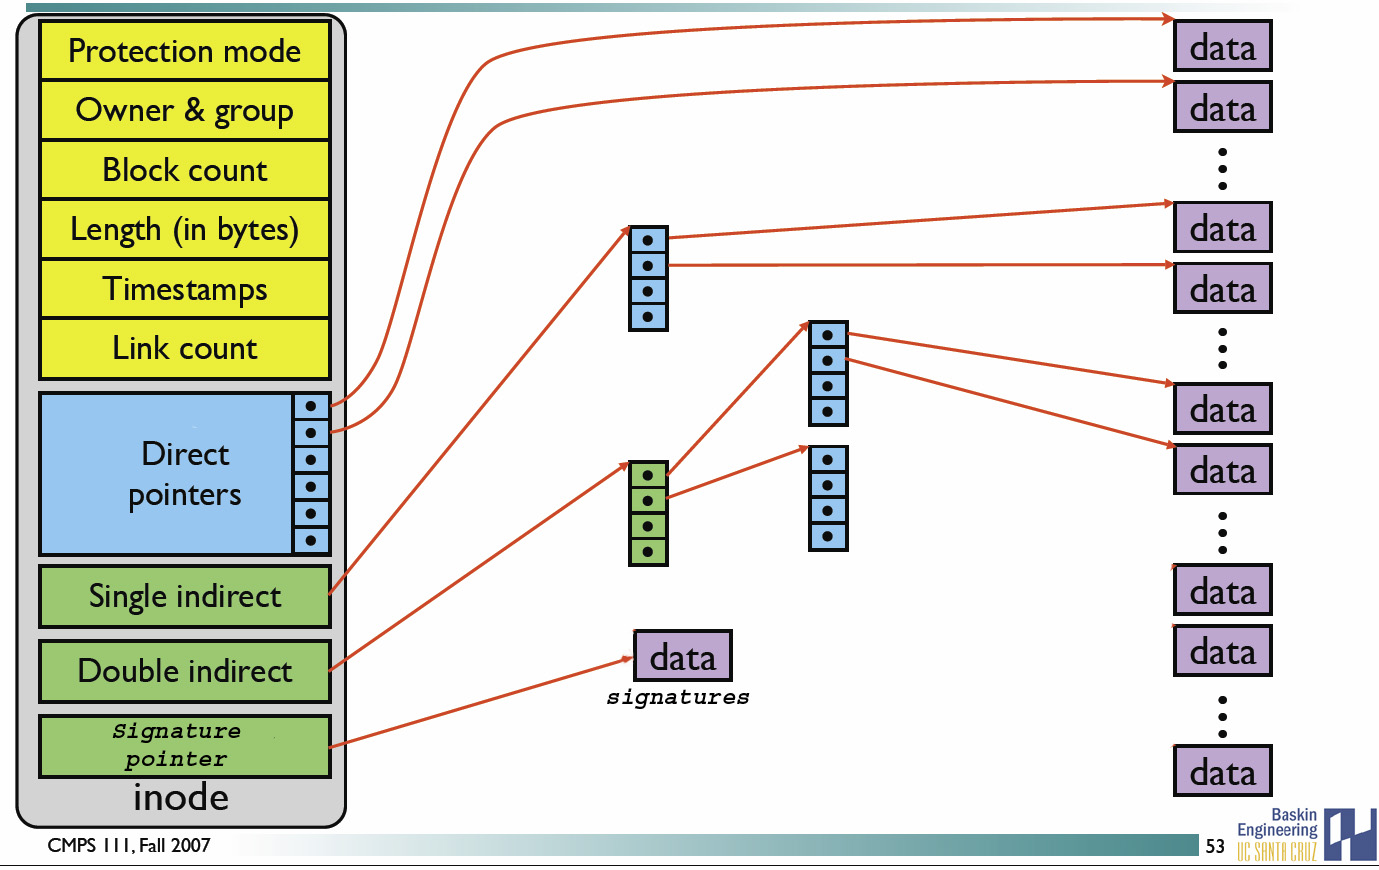
\includegraphics[width=.8\textwidth]{filesystems/images/inode_with_signatures.jpg}
\caption{Inode with contents}
\end{figure}

From \href{http://en.wikipedia.org/wiki/Inode}{Wikipedia}:

\begin{quote}
  \emph{In a Unix-style file system, an index node, informally referred to as an inode, is a data structure used to represent a filesystem object, which can be one of various things including a file or a directory.
    Each inode stores the attributes and disk block location(s) of the filesystem object's data.
    Filesystem object attributes may include manipulation metadata (e.g.~change, access, modify time), as well as owner and permission data (e.g.~group-id, user-id, permissions).}
\end{quote}

The superblock may store an array of inodes, each of which stores direct, and potentially several kinds of indirect pointers to disk blocks.
Since inodes are stored in the superblock, most filesystems have a limit on how many inodes can exist.
Since each inode corresponds to a file, this is also a limit on how many files that filesystem can have.
Trying to overcome this problem by storing inodes in some other location greatly increases the complexity of the filesystem.
Trying to reallocate space for the inode table is also infeasible since every byte following the end of the inode array would have to be shifted, a highly expensive operation.
This isn't to say there aren't any solutions at all, although typically there is no need to increase the number of inodes since the number of inodes is usually sufficiently high.

Big idea: Forget names of files.
The `inode' is the file.

It is common to think of the file name as the `actual' file.
It's not!
Instead, consider the inode as the file.
The inode holds the meta-information (last accessed, ownership, size) and points to the disk blocks used to hold the file contents.
However, the inode does not usually store a filename.
Filenames are usually only stored in directories (see below).

For example, to read the first few bytes of the file, follow the first direct block pointer to the first direct block and read the first few bytes.
Writing follows the same process.
If you want to read the entire file, keep reading direct blocks until you've read a number of bytes equal to the size of the file.
If the total size of the file is less than that of the number of direct blocks multiplied by the size of a block, then unused block pointers will be undefined.
Similarly, if the size of a file is not a multiple of the size of a block, data past the end of the last byte in the last block will be garbage.

What if a file is bigger than the maximum space addressable by it's direct blocks?
To that, we present a motto programmers take too seriously.

\begin{quote}
``All problems in computer science can be solved by another level of indirection.'' - David Wheeler
\end{quote}

Except the problem of too many layers of indirection.

To solve this problem, we introduce \keyword{indirect blocks}.
A single indirect block is a block that store pointers to more data blocks.
Similarly, a double indirect block stores pointers to single indirect blocks, and the concept can be generalized to arbitrary levels of indirection.
This is a very important concept, as inodes are stored in the superblock, or some other structure in a well known location with a constant amount of space, indirection allows exponential increases in the amount of space an inode can keep track of.

As a worked example, suppose we divide the disk into 4KiB blocks and we want to address up to $2^{32}$ blocks.
The maximum disk size is $4KiB *2^{32} = 16TiB$ remember $2^{10} = 1024$.
A disk block can store $\frac{4KiB}{4B}$ possible pointers or 1024 pointers.
Four byte wide pointers are needed because we want to address 32 bits worth of blocks.
Each pointer refers to a 4KiB disk block, so you can refer up to $1024*4KiB = 4MiB$ of data.
For the same disk configuration, a double indirect block stores 1024 pointers to 1024 indirection tables.
Thus a double-indirect block can refer up to $1024 * 4MiB = 4GiB$ of data.
Similarly, a triple indirect block can refer up to 4TiB of data.
Naturally though, this is three times as slow for reading between blocks, due to increased levels of indirection.
The actual intra-block reading times don't change.

\subsection{Directory Implementation}

A directory is just a mapping of names to inode numbers.
It is typically just a normal file, but with some special bits set in its inode and a very specific structure for its contents.
POSIX provides a small set of functions to read the filename and inode number for each entry, which we will talk about in depth later in this chapter.

Let's think about what it looks like in the actual file system.
Theoretically, directories are just like actual files.
The disk blocks will contain \emph{directory entries} or \emph{dirents}.
What that means is that our disk block can look like this

\begin{verbatim}
| inode_num | name   | | ----------- | ------ |
| 2043567   | hi.txt | | ... |
\end{verbatim}

Each directory entry could either be a fixed size, or a variable length C-string.
It depends on how the particular filesystem implements it at the lower level.
To see a mapping of filenames to inode numbers on a POSIX system, from a shell, use \keyword{ls} with the \keyword{-i} option

\begin{verbatim}
# ls -i
12983989 dirlist.c      12984068 sandwich.c
\end{verbatim}

You can see later that this is a powerful abstraction.
One can have a file be multiple different names in a directory, or exist in multiple directories.

\subsection{UNIX Directory Conventions}

In standard UNIX filesystems the following entries are specially added on requests to read a directory.

\begin{enumerate}
  \item \keyword{.} represents the current directory
  \item \keyword{..} represents the parent directory
  \item \keyword{~~} is the name of the home directory usually
\end{enumerate}

Counterintuitively, \keyword{...} does not refer to the `grandparent' directory (parent of the parent).
Only the current directory and the parent directory have special aliases involving \keyword{.} (namely , \keyword{.} and \keyword{..}).
However, \keyword{...} \emph{could} however be the name of a file or directory on disk (You can try this with \texttt{mkdir ...}).
Confusingly, the shell \keyword{zsh} does interpret \keyword{...} as a handy shortcut to the grandparent directory (should it exist) while expanding shell commands.

Additional facts about name-related conventions:

\begin{enumerate}
    \item Files that start with '.' (a period) on disk are conventionally considered 'hidden' and will not be listed by programs like \keyword{ls} without additional flags (\keyword{-a}).
        This is not a feature of the filesystem, and programs may choose to ignore this.
    \item Some files may also start with a null byte.
            These are usually \emph{abstract UNIX sockets} and are used to prevent cluttering up the filesystem since they will be effectively hidden by any program not expecting them.
            They will, however, be listed by tools that detail information about sockets, so this is not a feature providing security.
    \item If you want to annoy your neighbor, create a file with the terminal bell character.
        Ever single time the file is listed (by calling `ls', for example), an audible bell will be heard.
\end{enumerate}

\subsection{Directory API}

While interacting with a file in C is typically done by using \keyword{open} to open the file and then \keyword{read} or \keyword{write} to interact with the file before calling \keyword{close} to release resources, directories have special calls such as, \keyword{opendir}, \keyword{closedir} and \keyword{readdir}.
There is no function \keyword{writedir} since typically that implies creating a file or link (for that you would just use something like \keyword{open} or \keyword{mkdir}).

To explore these functions, let's write a program to search the contents of a directory for a particular file.
The code below has a bug, try to spot it!

\begin{lstlisting}[language=C]
int exists(char *directory, char *name)  {
    struct dirent *dp;
    DIR *dirp = opendir(directory);
    while ((dp = readdir(dirp)) != NULL) {
        puts(dp->d_name);
        if (!strcmp(dp->d_name, name)) {
        return 1; /* Found */
        }
    }
    closedir(dirp);
    return 0; /* Not Found */
}
\end{lstlisting}

Did you find the bug?
It leaks resources!
If a matching filename is found then `closedir' is never called as part of the early return.
Any file descriptors opened, and any memory allocated, by opendir are never released.
This means eventually the process will run out of resources and an \keyword{open} or \keyword{opendir} call will fail.

The fix is to ensure we free up resources in every possible code path.

In the above code, this means calling \keyword{closedir} before \keyword{return 1}.
Forgetting to release resources is a common C programming bug because there is no support in the C language to ensure resources are always released with all code paths.


Given an open directory, after a call to \keyword{fork()}, either (XOR), the parent or the child can use \keyword{readdir()}, \keyword{rewinddir()} or \keyword{seekdir()}.
If both the parent and the child use the above, behavior is undefined.

There are two main gotchas and one consideration.
The \keyword{readdir} function returns ``.'' (current directory) and ``..'' (parent directory).
If you are looking for sub-directories, you need to explicitly exclude these directories.

For many applications, it's reasonable to check the current directory first before recursively searching sub-directories.
This can be achieved by storing the results in a linked list, or resetting the directory struct to restart from the beginning.

The following code attempts to list all files in a directory recursively.
As an exercise, try to identify the bugs it introduces.

\begin{lstlisting}[language=C]
void dirlist(char *path) {
  struct dirent *dp;
  DIR *dirp = opendir(path);
  while ((dp = readdir(dirp)) != NULL) {
     char newpath[strlen(path) + strlen(dp->d_name) + 1];
     sprintf(newpath,"%s/%s", newpath, dp->d_name);
     printf("%s\n", dp->d_name);
     dirlist(newpath);
  }
}

int main(int argc, char **argv) {
  dirlist(argv[1]);
  return 0;
}
\end{lstlisting}

Did you find all 5 bugs?

\begin{lstlisting}[language=C]
// Check opendir result (perhaps user gave us a path that can not be opened as a directory
if (!dirp) { perror("Could not open directory"); return; }

// +2 as we need space for the / and the terminating 0
char newpath[strlen(path) + strlen(dp->d_name) + 2];

// Correct parameter
sprintf(newpath,"%s/%s", path, dp->d_name);

// Perform stat test (and verify) before recursing
if (0 == stat(newpath,&s) && S_ISDIR(s.st_mode)) dirlist(newpath)

// Resource leak: the directory file handle is not closed after the while loop
closedir(dirp);
\end{lstlisting}

One final note of caution.
\keyword{readdir} is not thread-safe!
You shouldn't use the re-entrant version of the function.
Synchronizing the filesystem within a process is important, so use locks around \keyword{readdir}.

See the \href{https://linux.die.net/man/3/readdir}{man page of readdir} for more details.

\subsection{Linking}

Links are what force us to model a filesystem as a tree rather than a graph.
While modeling the filesystem as a tree would imply that every inode has a unique parent directory, links allow inodes to present themselves as files in multiple places, potentially with different names, thus leading to an inode having multiple parent directories.
There are two kinds of links:

\begin{enumerate}
    \item \keyword{Hard Links}
        A hard link is simply an entry in a directory assigning some name to an inode number that already has a different name and mapping in either the same directory or a different one.
        If we already have a file on a file system we can create another link to the same inode using the \keyword{`ln'} command:

        \begin{lstlisting}[language=bash]
            $ ln file1.txt blip.txt
        \end{lstlisting}

        However, blip.txt \emph{is} the same file.
        If I edit blip, I'm editing the same file as `file1.txt!'.
        We can prove this by showing that both file names refer to the same inode.

        \begin{verbatim}
        $ ls -i file1.txt blip.txt
        134235 file1.txt
        134235 blip.txt
        \end{verbatim}

        The equivalent C call is \keyword{link}

        \begin{lstlisting}[language=C]
        // Function Prototype
        int link(const char *path1, const char *path2);

        link("file1.txt", "blip.txt");
        \end{lstlisting}

        For simplicity, the above examples made hard links inside the same directory.
        Hard links can be created anywhere inside the same filesystem.

    \item \keyword{Soft Links}
        The second kind of link is a soft link - or a symbolic link or a symlink.
        A symbolic link is different because it does not deal with inode numbers directly.
        Instead, a symbolic link is a file on disk with a special bit set and stores a path to another file.
        Quite simply, without the special bit, it is nothing more than a text file with a file path inside.
        Note when people generally talk about a link without specifying hard or soft, they are referring to a hard link.

        To create a symbolic link in the shell, use \keyword{ln -s}.
        To read the contents of the link as just a file, use \keyword{readlink}.
        These are both demonstrated below.

        \begin{verbatim}
            $ ln -s file1.txt file2.txt
            $ ls -i file1.txt blip.txt
            134235 file1.txt
            134236 file2.txt
            134235 blip.txt
            $ cat file1.txt
            file1!
            $ cat file2.txt
            file1!
            $ cat blip.txt
            file1!
            $ echo edited file2 >> file2.txt # >> is bash syntax for append to file
            $ cat file1.txt
            file1!
            edited file2
            $ cat file2.txt
            I'm file1!
            edited file2
            $ cat blip.txt
            file1!
            edited file2
            $ readlink myfile.txt
            file2.txt
        \end{verbatim}

        Note that \keyword{file2.txt} and \keyword{file1.txt} have different inode numbers, unlike the hard link, \keyword{blip.txt}.

        There is a C library call to create symlinks which is similar to link.

        \begin{lstlisting}[language=C]
        symlink(const char *target, const char *symlink);
        \end{lstlisting}

        Some advantages of symbolic links are

        \begin{itemize}
            \tightlist
                \item Can refer to files that don't exist yet
                \item Unlike hard links, can refer to directories as well as regular files
                \item Can refer to files (and directories) that exist outside of the current file system
        \end{itemize}

        However, symlinks have a key disadvantage, they as slower than regular files and directories.
        When the links contents are read, they must be interpreted as a new path to the target file, resulting in an additional call to open and read since the real file must be opened and read.
        Another disadvantage is that POSIX will not let you hard link directories whereas soft links are allowed.
        The \keyword{ln} command will only allow root to do this and only if you provide the \keyword{-d} option.
        However, even root may not be able to perform this because most filesystems prevent it!
\end{enumerate}

The integrity of the file system assumes the directory structure is an acyclic tree that is reachable from the root directory.
It becomes expensive to enforce or verify this constraint if directory linking is allowed.
Breaking these assumptions can cause file integrity tools to not be able to repair the file system.
Recursive searches potentially never terminate and directories can have more than one parent but ``..'' can only refer to a single parent.
All in all, a bad idea.
Soft links are merely ignored, which is why we can use them to reference directories.

When you remove a file using \keyword{rm} or \keyword{unlink}, you are removing an inode reference from a directory.
However the inode may still be referenced from other directories.
In order to determine if the contents of the file are still required, each inode keeps a reference count that is updated whenever a new link is created or destroyed.
This count only tracks hard links, symlinks are allowed to refer to a non-existent file and thus, do not matter.

An example use of hard links is to efficiently create multiple archives of a file system at different points in time.
Once the archive area has a copy of a particular file, then future archives can re-use these archive files rather than creating a duplicate file.
This is called an incremental backup.
Apple's ``Time Machine'' software does this.

\subsection{Pathing}

Now that we have definitions, and have talked about directories, we come across the concept of a path.
A path is a sequence of directories that provide one with a "path" in the graph that is a filesystem.
However, there are some nuances.
It is possible to have a path called \texttt{a/b/../c/./}.
Since \keyword{..} and \keyword{.} are special entries in directories, this is a valid path that actually refers to \texttt{a/c}.
Most filesystem functions will allow uncompressed paths to be passed in.
The C library provides a function \keyword{realpath} to compress the path or get the absolute path.
To simplify by hand, remember that \keyword{..} means `parent folder' and that \keyword{.} means `current folder'.
Below is an example that illustrates the simplification of the \texttt{a/b/../c/.} by using \keyword{cd} in a shell to navigate a filesystem.

\begin{enumerate}
  \item \keyword{cd a} (in a)
  \item \keyword{cd b} (in a/b)
  \item \keyword{cd ..} (in a, because .. represents `parent folder')
  \item \keyword{cd c} (in a/c)
  \item \keyword{cd .} (in a/c, because . represents `current folder')
\end{enumerate}

Thus, this path can be simplified to \keyword{a/c}.

\subsection{Metadata}

How can we distinguish between a regular file and a directory?
For that matter there's many other attributes that files also might contain.
We distinguish a file type -- different from the file extension i.e. png, svg, pdf -- using fields inside the inode.
How does the system know what type the file is?

This information is stored within an inode.
To access it, use the stat calls.
For example, to find out when my `notes.txt' file was last accessed.

\begin{lstlisting}[language=C]
struct stat s;
stat("notes.txt", &s);
printf("Last accessed %s", ctime(&s.st_atime));
\end{lstlisting}

There are actually three versions of \keyword{stat};

\begin{lstlisting}[language=C]
int stat(const char *path, struct stat *buf);
int fstat(int fd, struct stat *buf);
int lstat(const char *path, struct stat *buf);
\end{lstlisting}

For example, you can use \keyword{fstat} to learn about file metadata if you already have a file descriptor associated with that file.

\begin{lstlisting}[language=C]
FILE *file = fopen("notes.txt", "r");
int fd = fileno(file); /* Just for fun - extract the file descriptor from a C FILE struct */
struct stat s;
fstat(fd, & s);
printf("Last accessed %s", ctime(&s.st_atime));
\end{lstlisting}

\keyword{lstat} is almost the same as \keyword{stat} but handles symbolic links differently.
From the \keyword{stat} man page.

\begin{quote}
    lstat() is identical to stat(), except that if pathname is a symbolic link, then it returns information about the link itself, not the file that it refers to.
\end{quote}

The stat functions make use of \keyword{struct stat}.
From the \keyword{stat} man page:

\begin{lstlisting}[language=C]
struct stat {
    dev_t     st_dev;         /* ID of device containing file */
    ino_t     st_ino;         /* Inode number */
    mode_t    st_mode;        /* File type and mode */
    nlink_t   st_nlink;       /* Number of hard links */
    uid_t     st_uid;         /* User ID of owner */
    gid_t     st_gid;         /* Group ID of owner */
    dev_t     st_rdev;        /* Device ID (if special file) */
    off_t     st_size;        /* Total size, in bytes */
    blksize_t st_blksize;     /* Block size for filesystem I/O */
    blkcnt_t  st_blocks;      /* Number of 512B blocks allocated */
    struct timespec st_atim;  /* Time of last access */
    struct timespec st_mtim;  /* Time of last modification */
    struct timespec st_ctim;  /* Time of last status change */
};
\end{lstlisting}

The \keyword{st\_mode} field can be used to distinguish between regular files and directories.
To accomplish this, you will also need the macros, \keyword{S\_ISDIR} and \keyword{S\_ISREG}.

\begin{lstlisting}[language=C]
struct stat s;
if (0 == stat(name, &s)) {
  printf("%s ", name);
  if (S_ISDIR( s.st_mode)) puts("is a directory");
  if (S_ISREG( s.st_mode)) puts("is a regular file");
} else {
  perror("stat failed - are you sure I can read this file's meta data?");
}
\end{lstlisting}

\section{Permissions and bits}

Permissions are a key part of the way UNIX systems provide security in a filesystem.
You may have noticed that the \keyword{st\_mode} field in \keyword{struct stat} contains more than just the file type.
It also contains the mode, a description detailing what a user can and can't do with a given file.
There are usually three sets of permissions for any file.
Permissions for the \emph{user}, the \emph{group} and \emph{other} (everyone not covered by the first two categories).
For each of the three categories we need to keep track of whether or not the user is allowed to read the file, write to the file, and execute the file.
Since there are three categories and three permissions, permissions are usually represented as a 3-digit octal number.
For each digit, the least significant byte corresponds to read privileges, the middle one to write privileges and the final byte to execute privileges.
They are always presented as \emph{User}, \emph{Group}, \emph{Other} (\emph{UGO}).
Below are some common examples.
Here are the bit conventions:

\begin{enumerate}
\item \keyword{r} means that the set of people can read
\item \keyword{w} means that the set of people can write
\item \keyword{x} means that the set of people can execute
\end{enumerate}

\begin{tabular}{|c|c|c|c|}
  Octal Code & User & Group & Others \\ \hline
  755 & \keyword{rwx} & \keyword{r-x} & \keyword{r-x} \\
  644 & \keyword{rw-} & \keyword{r--} & \keyword{r--}
\end{tabular}

It is worth noting that the \keyword{rwx} bits have a slightly different meaning for directories.
Write access to a directory will allow you to create or delete new files or directories inside.
You can think about this as just having write access to the directory entry (dirent) mappings.
Read-access to a directory will allow you to list a directory's contents.
This is just read access to the directory entry (dirent) mapping.
Execute will allow you to enter the directory and access it.
Without the execute bit, it is not possible to create or remove files or directories since you cannot access them.
You can, however, list the contents of the directory.

There are several command line utilities for interacting with a file's mode.
\keyword{mknod} changes the type of the file.
\keyword{chmod} takes a number and a file and changes the permission bits.
However, before we can discuss chmod in detail, we must also understand the user ID (\keyword{uid}) and group id (\keyword{gid}) as well.

\subsection{User ID / Group ID}

Every user in a UNIX system has a user ID.
This is a unique number that can identify a user.
Similarly, users can be added to collections called groups, and every group also has a uniquely identifying number.
Groups have a variety of uses on UNIX systems.
They can be assigned capabilities - a way of describing the level of control a user has over a system.
For example, a group you may have run into is the \keyword{sudoers} group, a set of trusted users who are allowed to use the command \keyword{sudo} to temporarily gain higher privileges.
We'll talk more about how \keyword{sudo} works in this chapter.
Every file, upon creation, an owner, the creator of the file.
This owner's user ID (\keyword{uid}) can be found inside the \keyword{st\_mode} file of a \keyword{struct stat} with a call to \keyword{stat}.
Similarly, the group ID (\keyword{gid}) is set as well.

Every process can determine its \keyword{uid} and \keyword{gid} with \keyword{getuid} and \keyword{getgid}.
When a processes tries to open a file with a specific mode, it's \keyword{uid} and \keyword{gid} are compared with the \keyword{uid} and \keyword{gid} of the file.
If the \keyword{uid}s match, then the process's request to open the file will be compared with the bits on the user field of the file's permissions.
Similarly if the \keyword{gid}s match, then the process's request will be compared with the group field of the permissions.
Finally if none of the IDs match, then the other field will apply.

\subsection{Reading / Changing file permissions}

Before we discuss how to change permission bits, we should be able to read them.
In C, the \keyword{stat} family of library calls can be used.
To read permission bits from the command line, use \keyword{ls -l}.
Note, the permissions will outputted in the format `trwxrwxrwx'.
The first character indicates the type of file type.
Possible values for the first character include but aren't limited to.

\begin{enumerate}
    \item (-) regular file
    \item (d) directory
    \item (c) character device file
    \item (l) symbolic link
    \item (p) named pipe (also called FIFO)
    \item (b) block device
    \item (s) socket
\end{enumerate}

Alternatively, use the program \keyword{stat} which presents all the information that one could retrieve from the \keyword{stat} library call.

To change the permission bits, there is a system call, \keyword{int chmod(const char *path, mode\_t mode);}.
In order to simplify our examples, we will be using the command line utility of the same name \keyword{chmod} short of ``change mode''.
There are two common ways to use \keyword{chmod}, with either an octal value or with a symbolic string.

\begin{verbatim}
$ chmod 644 file1
$ chmod 755 file2
$ chmod 700 file3
$ chmod ugo-w file4
$ chmod o-rx file4
\end{verbatim}

The base-8 (`octal') digits describe the permissions for each role: The user who owns the file, the group and everyone else.
The octal number is the sum of three values given to the three types of permission: read(4), write(2), execute(1)

Example: \keyword{chmod 755 myfile}

\begin{enumerate}
\item r + w + x = digit * user has 4+2+1, full permission
\item group has 4+0+1, read and execute permission
\item all users have 4+0+1, read and execute permission
\end{enumerate}

\subsection{Understanding the `umask'}

The umask \emph{subtracts} (reduces) permission bits from \keyword{777} and is used when new files and new directories are created by open, mkdir etc.
By default the umask is set to \keyword{022} (octal), which means that group and other privileges will not include the writable bit .
Each process has a current umask value.
When forking, the child inherits the parent's umask value.

For example, by setting the umask to \keyword{077} in the shell, ensures that future file and directory creation will only be accessible to the current user,

\begin{verbatim}
$ umask 077
$ mkdir secretdir
\end{verbatim}

As a code example, suppose a new file is created with \keyword{open()} and mode bits \keyword{666} (write and read bits for user, group and other):

\begin{lstlisting}[language=C]
open("myfile", O_CREAT, S_IRUSR | S_IWUSR | S_IRGRP | S_IWGRP | S_IROTH | S_IWOTH);
\end{lstlisting}

If umask is octal \keyword{022}, then the permissions of the created file will be \keyword{0666} \& \textasciitilde{}\keyword{022} for example.

\begin{lstlisting}[language=C]
S_IRUSR | S_IWUSR | S_IRGRP | S_IROTH
\end{lstlisting}

\subsection{The `setuid' bit}

You may have noticed an additional bit that files with execute permission may have set.
This bit is the \keyword{setuid} bit.
It indicated that when run, the program will set the uid of the user to that of the owner of the file.
Similar, there is a \keyword{setgid} bit which sets the gid of the executor to the gid of the owner.
The canonical example of a program with \keyword{setuid} set is \keyword{sudo}.

\keyword{sudo} is usually a program that is owned by the root user - a user that has all capabilities.
By using \keyword{sudo} an otherwise unprivileged user can gain access to most parts of the system.
This is useful for running programs that may require elevated privileges, such as using \keyword{chown} to change ownership of a file, or to use \keyword{mount} to mount or unmount filesystems (an action we will discuss later in this chapter).
Here are some examples:

\begin{verbatim}
$ sudo mount /dev/sda2 /stuff/mydisk
$ sudo adduser fred
$ ls -l /usr/bin/sudo
-r-s--x--x  1 root  wheel  327920 Oct 24 09:04 /usr/bin/sudo
\end{verbatim}

When executing a process with the setuid bit, it is still possible to determine a user's original uid with \keyword{getuid}.
The real action of the \keyword{setuid} bit is to set the effective user ID (\keyword{euid}) which can be determined with \keyword{geteuid}.
The actions of \keyword{getuid} and \keyword{geteuid} are described below.

\begin{itemize}
\tightlist
\item
  \keyword{getuid} returns the real user id (zero if logged in as root)
\item
  \keyword{geteuid} returns the effective user id (zero if acting as root, e.g.~due to the setuid flag set on a program)
\end{itemize}

These functions can allow one to write a program that can only be run by a privileged user by checking \keyword{geteuid} or go a step further and ensure that the only user who can run the code is root by using \keyword{getuid}.

\subsection{The `sticky' bit}

Sticky bits as we use them today do not serve the same purpose as their initial introduction.
Sticky bits were a bit that could be set on an executable file that would allow a program's text segment to remain in swap even after the end of the program's execution.
This made subsequent executions of the same program faster.
Today, this behavior is no longer supported and the sticky bit only holds meaning when set on a directory,

When a directory's sticky bit is set only the file's owner, the directory's owner, and the root user can rename or delete the file.
This is useful when multiple users have write access to a common directory.
A common use of the sticky bit is for the shared and writable \keyword{/tmp} directory where many user's files may be stored, but users should not be able to access files belonging to other users.

To set the sticky bit, use \keyword{chmod +t}.

\begin{lstlisting}[language=bash]
aneesh$ mkdir sticky
aneesh$ chmod +t sticky
aneesh$ ls -l
drwxr-xr-x  7 aneesh aneesh    4096 Nov  1 14:19 .
drwxr-xr-x 53 aneesh aneesh    4096 Nov  1 14:19 ..
drwxr-xr-t  2 aneesh aneesh    4096 Nov  1 14:19 sticky
aneesh$ su newuser
newuser$ rm -rf sticky
rm: cannot remove 'sticky': Permission denied
newuser$ exit
aneesh$ rm -rf sticky
aneesh$ ls -l
drwxr-xr-x  7 aneesh aneesh    4096 Nov  1 14:19 .
drwxr-xr-x 53 aneesh aneesh    4096 Nov  1 14:19 ..
\end{lstlisting}

Note that in the example above, the username is prepended to the prompt, and the command \keyword{su} is used to switch users.

\section{Virtual filesystems and other filesystems}

POSIX systems, such as Linux and Mac OS X (which is based on BSD) include several virtual filesystems that are mounted (available) as part of the file-system.
Files inside these virtual filesystems do not exist on the disk.
They are generated dynamically by the kernel when a process requests a directory listing.
Linux provides 3 main virtual filesystems:

\begin{enumerate}
    \item /dev  - A list of physical and virtual devices (for example network card, cdrom, random number generator)
    \item /proc - A list of resources used by each process and (by tradition) set of system information
    \item /sys - An organized list of internal kernel entities
\end{enumerate}

For example if I want a continuous stream of 0s, I can run \keyword{cat /dev/zero}.

Another example is the file \keyword{/dev/null}, a great place to store bits that you never need to read!
Bytes sent to \keyword{/dev/null/} are never stored, but are simply discarded.
A common use of \keyword{/dev/null} is to discard standard output.
For example,

\begin{verbatim}
$ ls . >/dev/null
\end{verbatim}

\subsection{Managing files and filesystems}

Given the multitude of operations that are available to you from the filesystem, let's explore some tools and techniques that can be used to manage files and filesystems.

One example is creating a secure directory.
Suppose you created your own directory in /tmp and then set the permissions so that only you can use the directory (see below).
Is this secure?

\begin{verbatim}
$ mkdir /tmp/mystuff
$ chmod 700 /tmp/mystuff
\end{verbatim}

There is a window of opportunity between when the directory is created and when it's permissions are changed.
This leads to several vulnerabilities that are based on a race condition.

Another user replaces \keyword{mystuff} with a hard link to an existing file or directory owned by the second user, then they would be able to read and control the contents of the \keyword{mystuff} directory.
Oh no - our secrets are no longer secret!

However in this specific example, the \keyword{/tmp} directory has the sticky bit set, so other users may not delete the \keyword{mystuff} directory, and the simple attack scenario described above is impossible.
This does not mean that creating the directory and then later making the directory private is secure!
A better version is to atomically create the directory with the correct permissions from its inception.

\begin{lstlisting}[language=bash]
$ mkdir -m 700 /tmp/mystuff
\end{lstlisting}

\subsection{Obtaining random data}

\keyword{/dev/random} is a file which contains number generator where the entropy is determined from environmental noise.
Random will block/wait until enough entropy is collected from the environment.

\keyword{/dev/urandom} is like random, but differs in the fact that it allows for repetition (lower entropy threshold), thus won't block.


\subsection{Copying Files}

Use the versatile \keyword{dd} command.
For example, the following command copies 1 MiB of data from the file \keyword{/dev/urandom} to the file \keyword{/dev/null}.
The data is copied as 1024 blocks of block size 1024 bytes.

\begin{verbatim}
$ dd if=/dev/urandom of=/dev/null bs=1k count=1024
\end{verbatim}

Both the input and output files in the example above are virtual - they don't exist on a disk.
This means the speed of the transfer is unaffected by hardware power.

\keyword{dd} is also commonly used to make a copy of a disk or an entire filesystem to create images that can either be burned on to other disks or to distribute data to other users.

\subsection{Updating Modification Time}

The \keyword{touch} executable creates a file if it does not exist and also updates the file's last modified time to be the current time.
For example, we can make a new private file with the current time:

\begin{verbatim}
$ umask 077       # all future new files will mask out all r,w,x bits for group and other access
$ touch file123   # create a file if it does not exist, and update its modified time
$ stat file123
  File: `file123'
  Size: 0           Blocks: 0          IO Block: 65536  regular empty file
Device: 21h/33d Inode: 226148      Links: 1
Access: (0600/-rw-------)  Uid: (395606/ angrave)   Gid: (61019/     ews)
Access: 2014-11-12 13:42:06.000000000 -0600
Modify: 2014-11-12 13:42:06.001787000 -0600
Change: 2014-11-12 13:42:06.001787000 -0600
\end{verbatim}

An example use of touch is to force make to recompile a file that is unchanged after modifying the compiler options inside the makefile.
Remember that make is `lazy' - it will compare the modified time of the source file with the corresponding output file to see if the file needs to be recompiled.

\begin{verbatim}
$ touch myprogram.c   # force my source file to be recompiled
$ make
\end{verbatim}

\subsection{Managing Filesystems}

To manage filesystems on your machine, use \keyword{mount}.
Using mount without any options generates a list (one filesystem per line) of mounted filesystems including networked, virtual and local (spinning disk / SSD-based) filesystems.
Here is a typical output of mount

\begin{verbatim}
$ mount
/dev/mapper/cs241--server_sys-root on / type ext4 (rw)
proc on /proc type proc (rw)
sysfs on /sys type sysfs (rw)
devpts on /dev/pts type devpts (rw,gid=5,mode=620)
tmpfs on /dev/shm type tmpfs (rw,rootcontext="system_u:object_r:tmpfs_t:s0")
/dev/sda1 on /boot type ext3 (rw)
/dev/mapper/cs241--server_sys-srv on /srv type ext4 (rw)
/dev/mapper/cs241--server_sys-tmp on /tmp type ext4 (rw)
/dev/mapper/cs241--server_sys-var on /var type ext4 (rw)rw,bind)
/srv/software/Mathematica-8.0 on /software/Mathematica-8.0 type none (rw,bind)
engr-ews-homes.engr.illinois.edu:/fs1-homes/angrave/linux on /home/angrave type nfs (rw,soft,intr,tcp,noacl,acregmin=30,vers=3,sec=sys,sloppy,addr=128.174.252.102)
\end{verbatim}

Notice that each line includes the filesystem type source of the filesystem and mount point.
To reduce this output, we can pipe it into \keyword{grep} and only see lines that match a regular expression.

\begin{verbatim}
>mount | grep proc  # only see lines that contain 'proc'
proc on /proc type proc (rw)
none on /proc/sys/fs/binfmt_misc type binfmt_misc (rw)
\end{verbatim}

\subsubsection{Filesystem Mounting}

Suppose you had downloaded a bootable linux disk image from the \href{http://cosmos.cites.illinois.edu/pub/archlinux/iso/2015.04.01/archlinux-2015.04.01-dual.iso}{URL}

\begin{verbatim}
wget $URL
\end{verbatim}

Before putting the filesystem on a CD, we can mount the file as a filesystem and explore its contents.
Note: mount requires root access, so let's run it using sudo

\begin{verbatim}
$ mkdir arch
$ sudo mount -o loop archlinux-2015.04.01-dual.iso ./arch
$ cd arch
\end{verbatim}

Before the mount command, the arch directory is new and obviously empty.
After mounting, the contents of \keyword{arch/} will be drawn from the files and directories stored in the filesystem stored inside the \keyword{archlinux-2014.11.01-dual.iso} file.
The \keyword{loop} option is required because we want to mount a regular file not a block device such as a physical disk.

The loop option wraps the original file as a block device.
In this example, we will find out below that the file system is provided under \keyword{/dev/loop0}.
We can check the filesystem type and mount options by running the mount command without any parameters.
We will pipe the output into \keyword{grep} so that we only see the relevant output line(s) that contain `arch'.

\begin{verbatim}
$ mount | grep arch
/home/demo/archlinux-2014.11.01-dual.iso on /home/demo/arch type iso9660 (rw,loop=/dev/loop0)
\end{verbatim}

The iso9660 filesystem is a read-only filesystem originally designed for optical storage media (i.e.~CDRoms).
Attempting to change the contents of the filesystem will fail

\begin{verbatim}
$ touch arch/nocando
touch: cannot touch `/home/demo/arch/nocando': Read-only file system
\end{verbatim}

\section{Memory Mapped IO}

While we traditionally think of reading and writing from a file as operation that happen by using the \keyword{read} and \keyword{write} calls, there is an alternative, mapping a file into memory using \keyword{mmap}.
\keyword{mmap} can also be used for IPC, and you can see more about \keyword{mmap} as a system call that enables shared memory in the IPC chapter.
In this chapter, we'll briefly explore \keyword{mmap} as a filesystem operation.

\keyword{mmap} takes a file and maps its contents into memory.
This allows a user to treat the entire file as a buffer in memory for easier semantics while programming, and to avoid having to read a file as discrete chunks explicitly.

Not all filesystems support using \keyword{mmap} for IO, but amongst those that do, not all have the same behavior.
Some will simply implement \keyword{mmap} as a wrapper around \keyword{read} and \keyword{write}.
Others will add additional optimizations by taking advantage of the kernel's page cache.
Of course, such optimization can be used in the implementation of \keyword{read} and \keyword{write} as well, so often using \keyword{mmap} does not impact performance.

\keyword{mmap} is used to perform some operations such as loading libraries and processes into memory.
If many programs only need read-access to the same file, then the same physical memory can be shared between multiple processes.
This is used for common libraries like the C standard library.

The process to map a file into memory is as follows.

\begin{enumerate}
\item \keyword{mmap} requires a file descriptor, so we need to \keyword{open} the file first
\item We seek to our desired size and write one byte to ensure that the file is sufficient length
\item When finished call munmap to unmap the file from memory.
\end{enumerate}

Here is a quick example.

\begin{lstlisting}[language=C]
#include <stdio.h>
#include <stdlib.h>
#include <sys/types.h>
#include <sys/stat.h>
#include <sys/mman.h>
#include <fcntl.h>
#include <unistd.h>
#include <errno.h>
#include <string.h>


int fail(char *filename, int linenumber) {
  fprintf(stderr, "%s:%d %s\n", filename, linenumber, strerror(errno));
  exit(1);
  return 0; /*Make compiler happy */
}
#define QUIT fail(__FILE__, __LINE__ )

int main() {
  // We want a file big enough to hold 10 integers
  int size = sizeof(int) * 10;

  int fd = open("data", O_RDWR | O_CREAT | O_TRUNC, 0600); //6 = read+write for me!

  lseek(fd, size, SEEK_SET);
  write(fd, "A", 1);

  void *addr = mmap(0, size, PROT_READ | PROT_WRITE, MAP_SHARED, fd, 0);
  printf("Mapped at %p\n", addr);
  if (addr == (void*) -1 ) QUIT;

  int *array = addr;
  array[0] = 0x12345678;
  array[1] = 0xdeadc0de;

  munmap(addr,size);
  return 0;

}
\end{lstlisting}

The careful reader may notice that our integers were written in least-significant-byte format because that is the endianness of the CPU that we ran this example on.
We also allocated a file that is one byte too many! The \keyword{PROT\_READ | PROT\_WRITE} options specify the virtual memory protection.
The option \keyword{PROT\_EXEC} (not used here) can be set to allow CPU execution of instructions in memory.

\section{Reliable Single Disk Filesystems}

Most filesystems cache significant amounts of disk data in physical memory.
Linux, in this respect, is particularly extreme.
All unused memory is used as a giant disk cache.
The disk cache can have significant impact on overall system performance because disk I/O is slow.
This is especially true for random access requests on spinning disks where the disk read-write latency is dominated by the seek time required to move the read-write disk head to the correct position.

For efficiency, the kernel caches recently used disk blocks.
For writing, we have to choose a trade-off between performance and reliability.
Disk writes can also be cached (``Write-back cache'') where modified disk blocks are stored in memory until evicted.
Alternatively a `write-through cache' policy can be employed where disk writes are sent immediately to the disk.
The latter is safer as filesystem modifications are quickly stored to persistent media but slower than a write-back cache.
If writes are cached then they can be delayed and efficiently scheduled based on the physical position of each disk block.
Note, this is a simplified description because solid state drives (SSDs) can be used as a secondary write-back cache.

Both solid state disks (SSD) and spinning disks have improved performance when reading or writing sequential data.
Thus, operating systems can often use a read-ahead strategy to amortize the read-request costs and request several contiguous disk blocks per request.
By issuing an I/O request for the next disk block before the user application requires the next disk block, the apparent disk I/O latency can be reduced.

If your data is important and needs to be force written to disk, call \keyword{sync} to request that a filesystem changes be written (flushed) to disk.
However, not all operating systems honor this request and even if the data is evicted from the kernel buffers the disk firmware use an internal on-disk cache or may not yet have finished changing the physical media.
Note, you can also request that all changes associated with a particular file descriptor are flushed to disk using \keyword{fsync(int fd)}.

If your operating system fails in the middle of an operation, most modern file systems do something called \textbf{journaling} that work around this.
What the file system does is before it completes a potentially expensive operation, is that it writes what it is going to do down in a journal.
In the case of a crash or failure, one can step through the journal and see which files are corrupt and fix them.
This is a way to salvage hard disks in cases there is critical data and there is no apparent backup.

Even though it is unlikely for your computer, programming for data centers means that disks fail every few seconds.
Disk failures are measured using ``Mean-Time-To-Failure (MTTF)''.
For large arrays, the mean failure time can be surprisingly short.
For example if the MTTF(single disk) = 30,000 hours, then the MTTF(1000 disks)= 30000/1000=30 hours or about a day and a half!

\subsection{RAID - Redundant Array of Inexpensive Disks}

One way to protect against this is to store the data twice! This is the main principle of a ``RAID-1'' disk array.
By duplicating the writes to a disk with writes to another backup disk, there are exactly two copies of the data.
If one disk fails, the other disk serves as the only copy until it can be re-cloned.
Reading data is faster since data can be requested from either disk, but writes are potentially twice as slow because now two write commands need to be issued for every disk block write.
Compared to using a single disk, the cost of storage per byte has doubled.

Another common RAID scheme is RAID-0, meaning that a file could be split up among two disks, but if any one of the disks fail then the files are irrecoverable.
This has the benefit of halving write times because one part of the file could be writing to hard disk one and another part to hard disk two.


It is also common to combine these systems.
If you have a lot of hard disks, consider RAID-10.
This is where you have two systems of RAID-1, but the systems are hooked up in RAID-0 to each other.
This means you would get roughly the same speed from the slowdowns but now any one disk can fail and you can recover that disk.
If two disks from opposing raid partitions fail, there is a chance that recover can happen though we don't could on it most of the time.

\subsection{Higher Levels of RAID}

RAID-3 uses parity codes instead of mirroring the data.
For each N-bits written, we will write one extra bit, the `Parity bit' that ensures the total number of 1s written is even.
The parity bit is written to an additional disk.
If any one disk including the parity disk is lost, then its contents can still be computed using the contents of the other disks.

\begin{figure}[htbp]
\centering
\includegraphics{filesystems/images/raid.gif}
\caption{Raid diagram}
\end{figure}

One disadvantage of RAID-3 is that whenever a disk block is written, the parity block will always be written too.
This means that there is effectively a bottleneck in a separate disk.
In practice, this is more likely to cause a failure because one disk is being used 100\% of the time and once that disk fails then the other disks are more prone to failure.

A single disk failure will not result in data loss because there is sufficient data to rebuild the array from the remaining disks.
Data-loss will occur when two disks are unusable because there is no longer sufficient data to rebuild the array.
We can calculate the probability of a two disk failure based on the repair time which includes not just the time to insert a new disk but the time required to rebuild the entire contents of the array.

\begin{verbatim}
MTTF = mean time to failure
MTTR = mean time to repair
N = number of original disks

p = MTTR / (MTTF-one-disk / (N-1))
\end{verbatim}

Using typical numbers (MTTR=1day, MTTF=1000days, N-1 = 9, p=0.009)

There is a 1\% chance that another drive will fail during the rebuild process (at that point you had better hope you still have an accessible backup of your original data.
In practice, the probability of a second failure during the repair process is likely higher because rebuilding the array is I/O-intensive (and on top of normal I/O request activity).
This higher I/O load will also stress the disk array.

RAID-5 is similar to RAID-3 except that the check block (parity information) is assigned to different disks for different blocks.
The check-block is `rotated' through the disk array.
RAID-5 provides better read and write performance than RAID-3 because there is no longer the bottleneck of the single parity disk.
The one drawback is that you need more disks to have this setup and there are more complicated algorithms need to be used.

\begin{figure}[htbp]
\centering
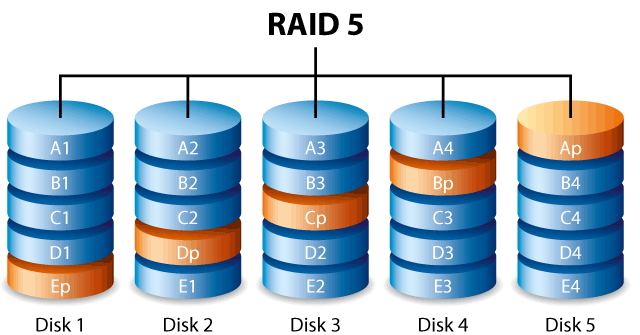
\includegraphics[width=.8\textwidth]{filesystems/images/raid_5.png}
\caption{Raid 5 striping}
\end{figure}

Failure is the common case.
Google reports 2-10\% of disks fail per year.
Multiplying that by 60,000+ disks in a single warehouse.
Services must survive failure of not just a disk, but a rack of servers or even a whole data center.

\subsection{Solutions}
Simple redundancy (2 or 3 copies of each file) e.g., Google GFS (2001).
More efficient redundancy (analogous to RAID 3++) e.g., \href{http://goo.gl/LwFIy}{Google Colossus filesystem} (\textasciitilde{}2010): customizable replication including Reed-Solomon codes with 1.5x redundancy

\section{Simple Filesystem Model}

Software developers need to implement filesystems all the time.
If that is surprising to you, we encourage you to take a look at Hadoop, GlusterFS, Qumulo, etc.
Filesystems are hot areas of research at the time of writing, because people have realized that the software models that we have devised don't take full advantage of our current hardware.
Additionally, the hardware that we use for storing information is getting better all the time.
As such, you may end up designing a filesystem yourself someday.
In this section, we will go over one of our fake filesystems that we talk about in class and ``walk through'' some examples of how things work.

So, what does our hypothetical filesystem look like? 
We will base it off of the \textt{minixfs}, a very simple filesystem that happens to be the first filesystem that Linux ran on.
It is laid out sequentially on disk, and the first section is the superblock.
The superblock stores important metadata about the entire filesystem.
Since we want to be able to read this block before we know anything else about the data on disk, this needs to be in a well-known location so the very start of the disk is a good choice.
After the superblock, we'll keep a map of which inodes are being used.
The nth bit is set if the nth inode -- $0$ being the inode root -- is being used.
Similarly, we store a map recording which data blocks are used.
Finally, we have an array of inodes followed by the rest of the disk - implicitly partitioned into data blocks.
It's important to note that there may not be any real distinction from one data block to the next from the perspective of the hardware components of the disk.
Thinking about the disk as an array of data blocks is simply something we do so that we have a way to describe where files live on disk.

Below, we have an example of how an inode that describes a file may look.
Note that for the sake of simplicity, we have drawn arrows mapping data block numbers in the inode to their locations on disk.
These aren't pointers so much as indices into an array.
\begin{figure}[htbp]
\centering
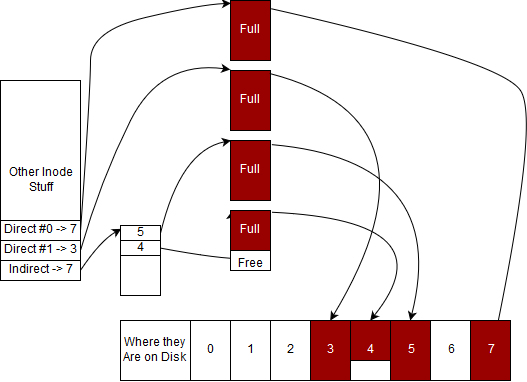
\includegraphics[width=.8\textwidth]{filesystems/images/sample_file.png}
\caption{Sample file filling up}
\end{figure}

We will assume that a data block is 4 KiB.

Note that a file will fill up each of its data blocks completely before requesting an additional data block.
We will refer to this property as as the file being \textit{compact}.
The file presented above is interesting since it uses all of it's direct blocks, one of the entries for it's indirect block and partially uses another indirect block.

The following subsections will all refer to the file presented above.

\subsection{How big is our file?}
The size of a file is not something that we can compute by staring at it's structure.
We need additional information that is typically stored in the inode.
This is because the filesystem isn't aware of the actual contents of what is in a file - that data is considered the user's and should only be manipulated by the user.
However, we can compute an upper and lower bounds on the filesize by only looking at how many blocks the file uses.

There are two full direct blocks, which together store $2*sizeof(data\_block)=2*4KiB=8KiB$.

There are two used blocks referenced by the indirect block, which can store up to $8KiB$ as calculated above.

We can now add these values to get an upper bound on the file size of $16KiB$.

What about a lower bound? We know that we must use the two direct blocks, one block referenced by the indirect block and at least 1 byte of a
second block referenced by the indirect block.
With this information, we can work out the lower bound to be $2*4KiB+4KiB+1=12KiB+1B$.

Note that our calculations so far have been to determine how much data the user is storing on disk.
We have not considered the \textit{overhead} of storing this data incurred while using this filesystem.
You'll notice that we use an indirect block to store the disk block numbers of blocks used beyond the two direct blocks.
While doing our above calculations, we did not take this block into account while computing the file size.
This would instead be counted as the overhead of the file, and thus the total overhead of storing this file on disk is $sizeof(indirect\_block)=4KiB)$.

Now that we're thinking about overhead, a related calculation could be to determine the max/min disk usage per file in this filesystem.

Trivially a file of size $0$ has no associated data blocks and takes up no space on disk (ignoring the space required for the inode since these are located in a fixed size array somewhere on disk).
How about the disk usage of the smallest non-empty file? That is, consider a file of size $1B$.
Note that when a user writes the first byte, a data block will be allocated.
Since each data block is $4KiB$, we find that $4KiB$ is the minimum disk usage for a non-empty file.
Here, we observe that the file size will only be $1B$, despite the fact that $4KiB$ of the disk is used -- there is a distinction between file size and disk usage because of overhead!

Finding maximum is slightly more involved.
As we saw earlier in this chapter, a filesystem with this structure can have $1024$ data block numbers in one indirect block.
This implies that the maximum filesize can be $2*4KiB + 1024*4KiB = 4MiB + 8KiB$ (after accounting for the direct blocks as well).
However, on disk we also store the indirect block itself.
This means that an additional $4KiB$ of overhead will be used to account for the indirect block, so the total disk usage will be $4MiB + 12KiB$.

Note that when only using direct blocks, completely filling up a direct block implies that our filesize and our disk usage are the same thing!
While it would seem like we always want this ideal scenario, it puts a very restrictive limit on the maximum filesize.
Attempting to remedy this by increasing the number of direct blocks seems promising, but note that this requires increasing the size of an inode and reducing the amount of space availible to store user data -- a tradeoff you will have to evaluate for yourself.
Alternatively always trying to split your data up into chunks that never use indirect blocks is also not necessarily wise since it could exhaust the limited pool of availible inodes.


\subsection{Performing Reads}

Performing reads tend to be pretty easy in our filesystem because our files are compact.
Let's say that we want to read the entirety of this particular file.
What we'd start by doing is go to the inode's direct struct and find the first direct data block number.
In our case it is \#7.
Then we find the 7th data block from the \textit{start} of all data blocks.
Then we read all of those bytes.
We do the same thing for all of the direct nodes.
What do we do after? 
We go to the indirect block and read the indirect block.
We know that every 4 bytes of the indirect block are either a sentinel node (-1) or the number of \textit{another} data block.
In our particular example, the first four bytes evaluate to the integer 5, meaning that our data continues on the 5th data block from the beginning.
We do the same for data block \#4 and we stop after because we exceed the size of the inode

Now, let's think about the edge cases.
How would you start the read starting at an arbitrary offset of $n$ bytes given that block sizes are $4 KiBs$.
How many indirect blocks should there be if the filesystem is correct? (Hint: \textit{think about using the size of the inode})

\subsection{Performing Writes}
\subsubsection{Writing to files}
Performing writes fall into two categories, writes to files and writes to directories.
First we'll focus on files and assume that we are writing a byte to the $6$th KiB of our file.
To perform a write on a file at a particular offset, first you must go to the data block would start at that offset.
For this particular example we would have to go to the 2nd or indexed number 1 inode to perform our write.
We would once again fetch this number from the inode, go to the root of the data blocks, go to the $5$th data block and perform our write at the $2$KiB offset from this block because we skipped the first four kibibytes of the file in block 7.
We perform our write and go on our merry way.

Some questions for you:

\begin {itemize}
    \item How would you consider performing a write that would go across data block boundaries?
    \item How would you consider performing a write whose write after adding the offset would extend the length of the file?\item How would you consider performing a write where the offset is greater than the length of the original file?
\end{itemize}

\subsubsection{Writing to directories}
Performing a write to a directory implies that an inode needs to be added to a directory.
If we pretend that the example above is a directory.
We know that we will be adding at most one directory entry at a time.
Meaning that we have to have enough space for one directory entry in our data blocks.
Luckily the last data block that we have has enough free space.
This means we just need to find the number of the last data block as we did above, go to where the data ends, and write one directory entry.
Don't forget to update the size of the directory so that the next creation doesn't overwrite your file!

Some more questions: 

\begin{itemize}
    \item How would you consider performing a write when the last data block is already full?
    \item How about when all the direct blocks have just been filled up and the inode doesn't have an indirect block?
    \item What about when the first indirect entry (\#4) is full?
\end{itemize}

These are edge cases you have to think about for a filesystem that really get you.

\subsection{Adding Deletes}

If you were to ask what happens when a file gets deleted, it is actually quite simple.
If the inode is a file, then remove the directory entry in the parent directory by marking it as invalid (maybe making it point to inode -1) and skip it in your reads.
You need to make sure to decrease the hard link count of the inode and if the count reaches zero, free the inode in the inode map and free all associated data blocks so they are reclaimed by the filesystem.
In many operating systems, several fields in the inode get overwritten.

If the inode is a directory, first you have to recursively remove every directory entry inside
After, you have to mark the directory's inode as free and set the associated data blocks to free as well.
Why don't we have to check hard link counts for directories?
You can't hard link directories! Meaning, we can just easily delete it.

\section{Topics}

\begin{itemize}
\tightlist
\item
  Superblock
\item
  Data Block
\item
  Inode
\item
  Relative Path
\item
  File Metadata
\item
  Hard and Soft Links
\item
  Permission Bits
\item
  Mode bits
\item
  Working with Directories
\item
  Virtual File System
\item
  Reliable File Systems
\item
  RAID
\end{itemize}

\section{Questions}

\begin{itemize}
\tightlist
\item
  How big can files be on a file system with 15 Direct blocks, 2 double, 3 triple indirect, 4kb blocks and 4byte entries? (Assume enough infinite blocks)
\item
  What is a superblock? Inode? Data block?
\item
  How do I simplify \keyword{/./proc/../dev/./random}/
\item
  In ext2, what is stored in an inode, and what is stored in a directory entry?
\item
  What are /sys, /proc, /dev/random, and /dev/urandom?
\item
  What are permission bits?
\item
  How do you use chmod to set user/group/owner read/write/execute permissions?
\item
  What does the ``dd'' command do?
\item
  What is the difference between a hard link and a symbolic link? Does the file need to exist?
\item
  ``ls -l'' shows the size of each file in a directory.
    Is the size stored in the directory or in the file's inode?
\end{itemize}

\bibliographystyle{plainnat}
\bibliography{filesystems/filesystems}

%\chapter{Signals}

\epigraph{What is that? It's ridiculous! [Jerry bobs agreeingly] You don't even know, what hotel she's staying at, you can't call her. That's a signal, Jerry, that's a signal! [snaps his fingers again] Signal!}{George Costanza (Seinfeld)}

Signals have been a unix construct since the beginning. They are a convenient way to deliver low-priority information and for users to interact with their programs when no other form of interaction is available like using standard input. Signals allow a program to cleanup or perform an action in the case of an event. Some time, a program can choose to ignore events and that is completely fine and even supported by the standard. Crafting a program that uses signals well is tricky due ot all the rules with inheritance. As such, signals are usually kept as cleanup or termination measures.

This chapter will go over how to first read information from a process that has either exited or been signaled and then it will deep dive into what are signals, how does the kernel deal with a signal, and the various ways processes can handle signals both in a single and multithreaded way.

\section{Exit statuses}

To find the return value of \keyword{main()} or value included in \keyword{exit()}), Use the \texttt{Wait macros} - typically you will use \keyword{WIFEXITED} and \keyword{WEXITSTATUS} . See \keyword{wait}/\keyword{waitpid} man page for more information.

\begin{code}[language=C]
int status;
pid_t child = fork();
if (child == -1) return 1; //Failed
if (child > 0) { /* I am the parent - wait for the child to finish */
  pid_t pid = waitpid(child, &status, 0);
  if (pid != -1 && WIFEXITED(status)) {
     int low8bits = WEXITSTATUS(status);
     printf("Process %d returned %d" , pid, low8bits);
  }
} else { /* I am the child */
 // do something interesting
  execl("/bin/ls", "/bin/ls", ".", (char *) NULL); // "ls ."
}
\end{code}

A process can only have 256 return values, the rest of the bits are informational, this is done by bit shifting. But, The kernel has an internal way of keeping track of signaled, exited, or stopped. That API is abstracted so that that the kernel developers are free to change at will. Remember that these macros only make sense if the precondition is met. Meaning that a process' exit status won't be defined if the process is signaled. The macros will not do the checking for you, so it's up to the programmer to make sure the logic checks out. As an example above, you should use the \keyword{WIFSTOPPED} to check if a process was stopped and then the \keyword{WSTOPSIG} to find the signal that stopped it. As such there is no need to memorize the following, this is just a high level overview of how information is stored inside the status variables. From \keyword{sys/wait.h} of an old Berkeley kernel\cite{sys/wait.h}:

\begin{code}[language=C]
/* If WIFEXITED(STATUS), the low-order 8 bits of the status. */
#define _WSTATUS(x) (_W_INT(x) & 0177)
#define _WSTOPPED 0177    /* _WSTATUS if process is stopped */
#define WIFSTOPPED(x) (_WSTATUS(x) == _WSTOPPED)
#define WSTOPSIG(x) (_W_INT(x) >> 8)
#define WIFSIGNALED(x)  (_WSTATUS(x) != _WSTOPPED && _WSTATUS(x) != 0)
#define WTERMSIG(x) (_WSTATUS(x))
#define WIFEXITED(x)  (_WSTATUS(x) == 0)
\end{code}

There is an untold convention about exit codes. If the process exited normally and everything was successful, then a zero should be returned. Beyond that, there isn't too many conventions except the ones that you place on yourself. If you know how the program you spawn is going to interact, you may be able to make more sense of the 256 error codes. You could in fact write your program to return \texttt{1} if the program went to stage 1 (like writing to a file) \texttt{2} if it did something else etc... But none of the unix programs are designed to follow that for simplicity sake.


\section{Signals}

A signal is a construct provided to us by the kernel. It allows one process to asynchronously send an event (think a message) to another process. If that process wants to accept the signal, it can, and then, for most signals, can decide what to do with that signal. Here is a short list (non comprehensive) of signals. The overall process for how a kernel sends a signal as well as common use cases are below.

\begin{enumerate}
\item Before any signals are generated, the kernel sets up the default signal handlers for a process.
\item If still no signals have arrived, the process can install its own signal handlers. This is simple telling the kernel that when the process gets signal X it should jump to function Y.
\item Now is the fun part, time to deliver a signal! Signals can come from various places below. The signal is now in what we call the generated state.
\item As soon as the signal starts to get deliverd by the kernel, it is in the pending state.
\item The kernel then checks the signals \keyword{disposition}, which in layperson terms is whether the process is willing to accept that signal at this point. If not, then the signal is currently blocked and nothing happens.
\item If not, and there is no signal handler installed, the kernel executes the default action. Otherwise, the kernel delivers the signal by stopping \textit{whatever} the process is doing at the current point, and jumping that process to the signal handler. If the program is multithreaded, then the process picks on thread with a signal disposition that can accept the signal and freezes the rest. The signal is now in the delivered phase.
\item Finally, we consider a signal caught if the process remains in tact after the signal was delivered.
\end{enumerate}

\begin{tableau}[c]{@{}lll@{}}
\toprule
\begin{minipage}[b]{0.12\columnwidth}\raggedright\strut
Name
\strut\end{minipage} &
\begin{minipage}[b]{0.44\columnwidth}\raggedright\strut
Default Action
\strut\end{minipage} &
\begin{minipage}[b]{0.35\columnwidth}\raggedright\strut
Usual Use Case
\strut\end{minipage}\tabularnewline
\midrule
\endhead
\begin{minipage}[t]{0.12\columnwidth}\raggedright\strut
SIGINT
\strut\end{minipage} &
\begin{minipage}[t]{0.44\columnwidth}\raggedright\strut
Terminate Process (Can be caught)
\strut\end{minipage} &
\begin{minipage}[t]{0.35\columnwidth}\raggedright\strut
Tell the process to stop nicely
\strut\end{minipage}\tabularnewline
\begin{minipage}[t]{0.12\columnwidth}\raggedright\strut
SIGQUIT
\strut\end{minipage} &
\begin{minipage}[t]{0.44\columnwidth}\raggedright\strut
Terminate Process (Can be caught)
\strut\end{minipage} &
\begin{minipage}[t]{0.35\columnwidth}\raggedright\strut
Tells the process to stop harshly
\strut\end{minipage}\tabularnewline
\begin{minipage}[t]{0.12\columnwidth}\raggedright\strut
SIGSTOP
\strut\end{minipage} &
\begin{minipage}[t]{0.44\columnwidth}\raggedright\strut
Stop Process (Cannot be caught)
\strut\end{minipage} &
\begin{minipage}[t]{0.35\columnwidth}\raggedright\strut
Stops the process to be continued
\strut\end{minipage}\tabularnewline
\begin{minipage}[t]{0.12\columnwidth}\raggedright\strut
SIGCONT
\strut\end{minipage} &
\begin{minipage}[t]{0.44\columnwidth}\raggedright\strut
Continues a Process
\strut\end{minipage} &
\begin{minipage}[t]{0.35\columnwidth}\raggedright\strut
Continues to run the process
\strut\end{minipage}\tabularnewline
\begin{minipage}[t]{0.12\columnwidth}\raggedright\strut
SIGKILL
\strut\end{minipage} &
\begin{minipage}[t]{0.44\columnwidth}\raggedright\strut
Terminate Process (Cannot be caught)
\strut\end{minipage} &
\begin{minipage}[t]{0.35\columnwidth}\raggedright\strut
You want your process gone
\strut\end{minipage}\tabularnewline
\bottomrule
\end{tableau}

\section{Sending Signals}

Signals can be genrated multiple ways. The user can send a signal. For example, you are at the terminal, and you send \keyword{CTRL-C} this is rarely the case in operating systems but is included in user programs for convenience. Another way is when a system event happens. For example, if you access a page that you aren't supposed to, the hardware generates a segfault interrupt which gets intercepted by the kernel. The kernel finds the process that caused this and sends a software interrupt signal \keyword{SIGSEGV}. There are softer kernel events like a child being created or sometimes when the kernel wants to like when it is scheduling processes. Finally, another process can send a message when you execute \keyword{kill\ -9\ PID}, it sends \keyword{SIGKILL} to the process. This could be used in low-stakes communication of events between process. If you are relying on signals to be the driver in your program, you should rethink your application design. There are many drawbacks to using signals for asynchronous communication that is avoided by having a dedicated thread and some form of proper Interprocess Communication.

You can temporarily pause a running process by sending it a SIGSTOP signal. If it succeeds it will freeze a process, the process will not be allocated any more CPU time. To allow a process to resume execution send it the SIGCONT signal. For example, Here's program that slowly prints a dot every second, up to 59 dots.

\begin{code}[language=C]
#include <unistd.h>
#include <stdio.h>
int main() {
  printf("My pid is %d\n", getpid() );
  int i = 60;
  while(--i) { 
    write(1, ".",1);
    sleep(1);
  }
  write(1, "Done!",5);
  return 0;
}
\end{code}

We will first start the process in the background (notice the \& at the end). Then send it a signal from the shell process by using the kill command.

\begin{code}[language=C]
>./program &
My pid is 403
...
>kill -SIGSTOP 403
>kill -SIGCONT 403
\end{code}

In C, you can send a signal to the child using \keyword{kill} POSIX call,

\begin{code}[language=C]
kill(child, SIGUSR1); // Send a user-defined signal
kill(child, SIGSTOP); // Stop the child process (the child cannot prevent this)
kill(child, SIGTERM); // Terminate the child process (the child can prevent this)
kill(child, SIGINT); // Equivalent to CTRL-C (by default closes the process)
\end{code}

As we saw above there is also a \keyword{kill} command available in the shell. Another command \keyword{killall} works the exact same way but instead of looking up by PID, it tries to match the name of the process. \keyword{ps} is an important utility that can help you find the pid of a process.

\begin{code}[language=console]
# First let's use ps and grep to find the process we want to send a signal to
$ ps au | grep myprogram
angrave  4409   0.0  0.0  2434892    512 s004  R+    2:42PM   0:00.00 myprogram 1 2 3

#Send SIGINT signal to process 4409 (equivalent of `CTRL-C`)
$ kill -SIGINT 4409

#Send SIGKILL (terminate the process)
$ kill -SIGKILL 4409
$ kill -9 4409
# Use kill all instead
$ killall -l firefox
\end{code}

In order to send a signal to the current, use \keyword{raise} or \keyword{kill} with \keyword{getpid()}

\begin{code}[language=C]
raise(int sig); // Send a signal to myself!
kill(getpid(), int sig); // Same as
\end{code}

For non-root processes, signals can only be sent to processes of the same user. You cant just SIGKILL my processes! \keyword{man -s2 kill} for more details.


\section{Handling Signals}

There are strict limitations on the executable code inside a signal handler. Most library and system calls are not \keyword{async-signal-safe} - they may not be used inside a signal handler because they are not re-entrant safe. Re-entrant safe means that imagine that your function can be frozen at any point and executed again, can you guarentee that your function wouldn't fail? Let's take the following

\begin{code}[language=C]
int func(const char *str) {
  static char buffer[200];
  strncpy(buffer, str, 199); # We finish this line and get recalled
  printf("%s\n", buffer)
}
\end{code}

\begin{enumerate}
\item We execute \keyword(func("Hello"))
\item The string gets copied over to the buffer completely (strcmp(buffer, "Hello") == 0)
\item A signal is deliverd and the function state freezes, we also stop accepting any new signals until after the handler (we do this for convenience)
\item We execute \keyword{func("World")}
\item Now (strcmp(buffer, "World") == 0) and the buffer is printed out "World".
\item We resume the interrupted function and now print out the buffer once again "World" instead of what the function call originally intended "Hello"
\end{enumerate}

Guarenteeing that your functions are signal handler safe are not as simple as not having shared buffers. You must also think about multithreading and synchronization i.e. what happens when I double lock a mutex? You also have to make sure that each subfunction call is re-entrant safe. Suppose your original program was interrupted while executing the library code of \keyword{malloc} ; the memory structures used by malloc will not be in a consistent state. Calling \keyword{printf} (which uses \keyword{malloc}) as part of the signal handler is unsafe and will result in \keyword{undefined behavior} i.e.~it is no longer a useful,predictable program. In practice your program might crash, compute or generate incorrect results or stop functioning (\keyword{deadlock}), depending on exactly what your program was executing when it was interrupted to execute the signal handler code. One common use of signal handlers is to set a boolean flag that is occasionally polled (read) as part of the normal running of the program. For example,

\begin{code}[language=C]
int pleaseStop ; // See notes on why "volatile sig_atomic_t" is better

void handle_sigint(int signal) {
  pleaseStop = 1;
}

int main() {
  signal(SIGINT, handle_sigint);
  pleaseStop = 0;
  while ( ! pleaseStop) { 
     /* application logic here */ 
   }
  /* cleanup code here */
}
\end{code}

The above code might appear to be correct on paper. However, we need to provide a hint to the compiler and to the CPU core that will execute the \keyword{main()} loop. We need to prevent a compiler optimization: The expression \keyword{!\ pleaseStop} appears to be a loop invariant meaning it will be true forever, so can be simplified to \keyword{true}. Secondly, we need to ensure that the value of \keyword{pleaseStop} is not cached using a CPU register and instead always read from and written to main memory. The \keyword{sig\_atomic\_t} type implies that all the bits of the variable can be read or modified as an \keyword{atomic operation} - a single uninterruptable operation. It is impossible to read a value that is composed of some new bit values and old bit values.

By specifying \keyword{pleaseStop} with the correct type \keyword{volatile\ sig\_atomic\_t}, we can write portable code where the main loop will be exited after the signal handler returns. The \keyword{sig\_atomic\_t} type can be as large as an \keyword{int} on most modern platforms but on embedded systems can be as small as a \keyword{char} and only able to represent (-127 to 127) values.

\begin{code}[language=C]
volatile sig_atomic_t pleaseStop;
\end{code}

Two examples of this pattern can be found in \keyword{COMP} a terminal based 1Hz 4bit computer \cite{Sorn_2015}. Two boolean flags are used. One to mark the delivery of \keyword{SIGINT} (CTRL-C), and gracefully shutdown the program, and the other to mark \keyword{SIGWINCH} signal to detect terminal resize and redraw the entire display.

You can also choose a handle pending signals asynchronously or synchronously. Install a signal handler to asynchronously handle signals use \keyword{sigaction} (or, for simple examples, \keyword{signal} ). To synchronously catch a pending signal use \keyword{sigwait} which blocks until a signal is delivered or \keyword{signalfd} which also blocks and provides a file descriptor that can be \keyword{read()} to retrieve pending signals.

\subsection{Sigaction}

You should use \keyword{sigaction} instead of \keyword{signal} because it has better defined semantics. \keyword{signal} on different operating system does different things which is \textbf{bad} \keyword{sigaction} is more portable and is better defined for threads if need be. To change the \keyword{signal disposition} of a process - i.e.~what happens when a signal is delivered to your process - use \keyword{sigaction} You can use system call \keyword{sigaction} to set the current handler for a signal or read the current signal handler for a particular signal.

\begin{code}[language=C]
int sigaction(int signum, const struct sigaction *act, struct sigaction *oldact);
\end{code}

The sigaction struct includes two callback functions (we will only look at the `handler' version), a signal mask and a flags field -

\begin{code}[language=C]
struct sigaction {
               void     (*sa_handler)(int);
               void     (*sa_sigaction)(int, siginfo_t *, void *);
               sigset_t   sa_mask;
               int        sa_flags;
}; 
\end{code}

Suppose you installed a signal handler for the alarm signal,

\begin{code}[language=C]
signal(SIGALRM, myhandler);
\end{code}

The equivalent \keyword{sigaction} code is:

\begin{code}[language=C]
struct sigaction sa; 
sa.sa_handler = myhandler;
sigemptyset(&sa.sa_mask);
sa.sa_flags = 0; 
sigaction(SIGALRM, &sa, NULL)
\end{code}

However, we typically may also set the mask and the flags field. The mask is a temporary signal mask used during the signal handler execution. The \keyword{SA\_RESTART} flag will automatically restart some (but not all) system calls that otherwise would have returned early (with EINTR error). The latter means we can simplify the rest of code somewhat because a restart loop may no longer be required.

\begin{code}[language=C]
sigfillset(&sa.sa_mask);
sa.sa_flags = SA_RESTART; /* Restart functions if  interrupted by handler */     
\end{code}

\subsection{Sigwait}

Sigwait can be used to read one pending signal at a time. \keyword{sigwait} is used to synchronously wait for signals, rather than handle them in a callback. A typical use of sigwait in a multi-threaded program is shown below. Notice that the thread signal mask is set first (and will be inherited by new threads). This prevents signals from being \emph{delivered} so they will remain in a pending state until sigwait is called. Also notice the same set sigset\_t variable is used by sigwait - except rather than setting the set of blocked signals it is being used as the set of signals that sigwait can catch and return.

One advantage of writing a custom signal handling thread (such as the example below) rather than a callback function is that you can now use many more C library and system functions that otherwise could not be safely used in a signal handler because they are not async signal-safe.

Based on Sigmask Code\cite{pthread_sigmask}

\begin{code}[language=C]
static sigset_t   signal_mask;  /* signals to block         */

int main (int argc, char *argv[]) {
    pthread_t sig_thr_id;      /* signal handler thread ID */
    sigemptyset (&signal_mask);
    sigaddset (&signal_mask, SIGINT);
    sigaddset (&signal_mask, SIGTERM);
    pthread_sigmask (SIG_BLOCK, &signal_mask, NULL);

    /* New threads will inherit this thread's mask */
    pthread_create (&sig_thr_id, NULL, signal_thread, NULL);

    /* APPLICATION CODE */
    ...
}

void *signal_thread (void *arg) {
    int       sig_caught;    /* signal caught       */

    /* Use same mask as the set of signals that we'd like to know about! */
    sigwait(&signal_mask, &sig_caught);
    switch (sig_caught)
    {
    case SIGINT:     /* process SIGINT  */
        ...
        break;
    case SIGTERM:    /* process SIGTERM */
        ...
        break;
    default:         /* should normally not happen */
        fprintf (stderr, "\nUnexpected signal %d\n", sig_caught);
        break;
    }
}
\end{code}

\section{Signal Disposition}

For each process, each signal has a disposition which means what action will occur when a signal is delivered to the process. For example, the default disposition SIGINT is to terminate it. The signal disposition can be changed by calling signal() (which is simple but not portable as there are subtle variations in its implementation on different POSIX architectures and also not recommended for multi-threaded programs) or \keyword{sigaction} (discussed later). You can imagine the processes' disposition to all possible signals as a table of function pointers entries (one for each possible signal).

The default disposition for signals can be to ignore the signal, stop the process, continue a stopped process, terminate the process, or terminate the process and also dump a `core' file. Note a core file is a representation of the processes' memory state that can be inspected using a debugger.

Multiple signals connot be queued. However it is possible to have signals that are in a pending state. If a signal is pending, it means it has not yet been delivered to the process. The most common reason for a signal to be pending is that the process (or thread) has currently blocked that particular signal. If a particular signal, e.g.~SIGINT, is pending then it is not possible to queue up the same signal again. It \emph{is} possible to have more than one signal of a different type in a pending state. For example SIGINT and SIGTERM signals may be pending (i.e.~not yet delivered to the target process)

Signals can be blocked (meaning they will stay in the pending state) by setting the process signal mask or, when you are writing a multi-threaded program, the thread signal mask.

\section{Disposition in Child Processes (No Threads)}

After forking, The child process inherits a copy of the parent's signal dispositions and a copy of the parent's signal mask. In other words, if you have installed a SIGINT handler before forking, then the child process will also call the handler if a SIGINT is delivered to the child. Also if \keyword{SIGINT} is blocked in the parent, it will be blocked in the child too. Note pending signals for the child are \emph{not} inherited during forking. But after \keyword{exec}, both the signal mask and the signal disposition carries over to the exec-ed program \cite{execute}. Pending signals are preserved as well. Signal handlers are reset, because the original handler code has disappeared along with the old process.

To block signals use \keyword{sigprocmask}! With sigprocmask you can set the new mask, add new signals to be blocked to the process mask, and unblock currently blocked signals. You can also determine the existing mask (and use it for later) by passing in a non-null value for oldset.

\begin{code}[language=C]
int sigprocmask(int how, const sigset_t *set, sigset_t *oldset);`
\end{code}

From the Linux man page of sigprocmask,

\begin{verbatim}
SIG_BLOCK: The set of blocked signals is the union of the current set and the 
  set argument.
SIG_UNBLOCK: The signals in set are removed from the current set of blocked 
  signals. It is permissible to attempt to unblock a signal which is not blocked.
SIG_SETMASK: The set of blocked signals is set to the argument set.
\end{verbatim}

The sigset type behaves as a bitmap, except functions are used rather than explicitly setting and unsetting bits using \& and \textbar{}. It is a common error to forget to initialize the signal set before modifying one bit. For example,

\begin{code}[language=C]
sigset_t set, oldset;
sigaddset(&set, SIGINT); // Ooops!
sigprocmask(SIG_SETMASK, &set, &oldset)
\end{code}

Correct code initializes the set to be all on or all off. For example,

\begin{code}[language=C]
sigfillset(&set); // all signals
sigprocmask(SIG_SETMASK, &set, NULL); // Block all the signals!
// (Actually SIGKILL or SIGSTOP cannot be blocked...)

sigemptyset(&set); // no signals 
sigprocmask(SIG_SETMASK, &set, NULL); // set the mask to be empty again
\end{code}


\section{Signals in a multithreaded program}

The new thread inherits a copy of the calling thread's mask. On initialization the calling thread's mask is the exact same as the processes mask because threads are essentially processes. After a new thread is created though, the processes signal mask turns into a gray area. Instead, the kernel likes to threat the process as a collection of thread, each of which can institute a signal mask and receive signals. In order to start setting your mask you can use,

\begin{code}[language=C]
pthread_sigmask( ... ); // set my mask to block delivery of some signals
pthread_create( ... ); // new thread will start with a copy of the same mask
\end{code}

Blocking signals is similar in multi-threaded programs to single-threaded programs: 
* Use \keyword{pthread\_sigmask} instead of \keyword{sigprocmask}
* Block a signal in all threads to prevent its asynchronous delivery

The easiest method to ensure a signal is blocked in all threads is to set the signal mask in the main thread before new threads are created

\begin{code}[language=C]
sigemptyset(&set);
sigaddset(&set, SIGQUIT);
sigaddset(&set, SIGINT);
pthread_sigmask(SIG_BLOCK, &set, NULL);

// this thread and the new thread will block SIGQUIT and SIGINT
pthread_create(&thread_id, NULL, myfunc, funcparam);
\end{code}

Just as we saw with \keyword{sigprocmask}, \keyword{pthread\_sigmask} includes a `how' parameter that defines how the signal set is to be used:

\begin{code}[language=C]
pthread_sigmask(SIG_SETMASK, &set, NULL) - replace the thread's mask with given signal set
pthread_sigmask(SIG_BLOCK, &set, NULL) - add the signal set to the thread's mask
pthread_sigmask(SIG_UNBLOCK, &set, NULL) - remove the signal set from the thread's mask
\end{code}

A signal then can delivered to any signal thread that is not blocking that signal. If the two or more threads can receive the signal then which thread will be interrupted is arbitrary! A common practice is to have one thread that can receive all signals or if there is a certain signal that requires special logic, have multiple threads for multiple signals. Even though programs from the outside can't send signals to specific threads (unless a thread is assigned a signal), you can do that in your program with \keyword{pthread\_kill(pthread\_t thread, int sig)}. In the example below, the newly created thread executing \keyword{func} will be interrupted by \keyword{SIGINT}

\begin{code}[language=C]
pthread_create(&tid, NULL, func, args);
pthread_kill(tid, SIGINT);
pthread_kill(pthread_self(), SIGKILL); // send SIGKILL to myself
\end{code}

As a word of warning \keyword{pthread\_kill(threadid, SIGKILL)} will kill the entire process. Though individual threads can set a signal mask, the signal disposition (the table of handlers/action performed for each signal) is \emph{per-proces}s not \emph{per-thread}. This means \keyword{sigaction} can be called from any thread because you will be setting a signal handler for all threads in the process.

The linux man pages discusses signal system calls in section 2. There is also a longer article in section 7 (though not in OSX/BSD):

\begin{code}[language=C]
man -s7 signal
\end{code}

\section{Topics}\label{topics}

\begin{itemize}
\tightlist
\item
  Signals
\item
  Signal Handler Safe
\item
  Signal Disposition
\item
  Signal States
\item
  Pending Signals when Forking/Exec
\item
  Signal Disposition when Forking/Exec
\item
  Raising Signals in C
\item
  Raising Signals in a multithreaded program
\end{itemize}

\section{Questions}\label{questions}

\begin{itemize}
\tightlist
\item
  What is a signal?
\item
  How are signals served under UNIX? (Bonus: How about Windows?)
\item
  What does it mean that a function is signal handler safe
\item
  What is a process Signal Disposition?
\item
  How do I change the signal disposition in a single threaded program?
  How about multithreaded?
\item
  Why sigaction vs signal?
\item
  How do I asynchronously and synchronously catch a signal?
\item
  What happens to pending signals after I fork? Exec?
\item
  What happens to my signal disposition after I fork? Exec?
\end{itemize}

\bibliographystyle{plainnat}
\bibliography{signals/signals}

%\chapter{Review}

A non-comprehensive list of topics is below.

\begin{enumerate}
\item CSP (critical section problems)
\item HTTP
\item SIGINT
\item TCP
\item TLB
\item Virtual Memory
\item arrays
\item barrier
\item c strings
\item chmod
\item client/server
\item coffman conditions
\item condition variables
\item context switch
\item deadlock
\item dining philosophers
\item epoll
\item exit
\item file I/O
\item file system representation
\item fork/exec/wait
\item fprintf
\item free
\item heap allocator
\item heap/stack
\item inode vs name
\item malloc
\item mkfifo
\item mmap
\item mutexes
\item network ports
\item open/close
\item operating system terms
\item page fault
\item page tables
\item pipes
\item pointer arithmetic
\item pointers
\item printing (printf)
\item producer/consumer
\item progress/mutex
\item race conditions
\item read/write
\item reader/writer
\item resource allocation graphs
\item ring buffer
\item scanf 
\item buffering
\item scheduling
\item select
\item semaphores
\item signals
\item sizeof
\item stat
\item stderr/stdout
\item symlinks
\item thread control (pthread\_create, pthread\_join, pthread\_exit)
\item variable initializers
\item variable scope
\item vm thrashing
\item wait macros
\item write/read with errno, EINTR and partial data
\end{enumerate}

\section{C}

\subsection{Memory and Strings}

\begin{enumerate}

\item In the example below, which variables are guaranteed to print the value of zero?

\begin{lstlisting}[language=C]
int a;
static int b;

void func() {
   static int c;
   int d;
   printf("%d %d %d %d\n",a,b,c,d);
}
\end{lstlisting}

\item In the example below, which variables are guaranteed to print the value of zero?

\begin{lstlisting}[language=C]
void func() {
   int* ptr1 = malloc( sizeof(int) );
   int* ptr2 = realloc(NULL, sizeof(int) );
   int* ptr3 = calloc( 1, sizeof(int) );
   int* ptr4 = calloc( sizeof(int) , 1);
   
   printf("%d %d %d %d\n",*ptr1,*ptr2,*ptr3,*ptr4);
}
\end{lstlisting}

\item Explain the error in the following attempt to copy a string.

\begin{lstlisting}[language=C]
char* copy(char*src) {
 char*result = malloc( strlen(src) ); 
 strcpy(result, src); 
 return result;
}
\end{lstlisting}

\item Why does the following attempt to copy a string sometimes work and sometimes fail?

\begin{lstlisting}[language=C]
char* copy(char*src) {
 char*result = malloc( strlen(src) +1 ); 
 strcat(result, src); 
 return result;
}
\end{lstlisting}

\item Explain the two errors in the following code that attempts to copy a string.

\begin{lstlisting}[language=C]
char* copy(char*src) {
 char result[sizeof(src)]; 
 strcpy(result, src); 
 return result;
}
\end{lstlisting}

\item Which of the following is legal?

\begin{lstlisting}[language=C]
char a[] = "Hello"; strcpy(a, "World");
char b[] = "Hello"; strcpy(b, "World12345", b);
char* c = "Hello"; strcpy(c, "World");
\end{lstlisting}

\item Complete the function pointer typedef to declare a pointer to a function that takes a void* argument and returns a void*. Name your type `pthread\_callback'

\begin{lstlisting}[language=C]
typedef ______________________;
\end{lstlisting}

\item In addition to the function arguments what else is stored on a thread's stack?

\item Implement a version of \texttt{char*\ strcat(char*dest,\ const\ char*src)} using only \texttt{strcpy} \texttt{strlen} and pointer arithmetic

\begin{lstlisting}[language=C]
char* mystrcat(char*dest, const char*src) {

  ? Use strcpy strlen here

  return dest;
}
\end{lstlisting}

\item Implement version of size\_t strlen(const char*) using a loop and no function calls.

\begin{lstlisting}[language=C]
size_t mystrlen(const char*s) {

}
\end{lstlisting}

\item Identify the three bugs in the following implementation of \texttt{strcpy}.

\begin{lstlisting}[language=C]
char* strcpy(const char* dest, const char* src) {
  while(*src) { *dest++ = *src++; }
  return dest;
}
\end{lstlisting}

\end{enumerate}

\subsection{Printing}

\begin{enumerate}

\item Spot the two errors!

\begin{lstlisting}[language=C]
fprintf("You scored 100%");
\end{lstlisting}

\item Complete the following code to print to a file. Print the name, a comma and the score to the file `result.txt'

\begin{lstlisting}[language=C]
char* name = .....;
int score = ......
FILE *f = fopen("result.txt",_____);
if(f) {
    _____
}
fclose(f);
\end{lstlisting}

\item How would you print the values of variables a,mesg,val and ptr to a string? Print a as an integer, mesg as C string, val as a double val and ptr as a hexadecimal pointer. You may assume the mesg points to a short C string(\textless{}50 characters). Bonus: How would you make this code more robust or able to cope with?

\begin{lstlisting}[language=C]
char* toString(int a, char*mesg, double val, void* ptr) {
   char* result = malloc( strlen(mesg) + 50);
    _____
   return result;
}
\end{lstlisting}

\end{enumerate}

\subsection{Input parsing}

\begin{enumerate}
\item Why should you check the return value of sscanf and scanf? \#\# Q 5.2 Why is `gets' dangerous?

\item Write a complete program that uses \texttt{getline}. Ensure your program has no memory leaks.

\item When would you use calloc not malloc? When would realloc be useful?

\item What mistake did the programmer make in the following code? Is it possible to fix it 

i) using heap memory?
ii) using global (static) memory?

\begin{lstlisting}[language=C]
static int id;

char* next_ticket() {
  id ++;
  char result[20];
  sprintf(result,"%d",id);
  return result;
}
\end{lstlisting}

\end{enumerate}

\section{Threading}

\begin{enumerate}

\item Is the following code thread-safe? Redesign the following code to be thread-safe. Hint: A mutex is unnecessary if the message memory is unique to each call.

\begin{lstlisting}[language=C]
static char message[20];
pthread_mutex_t mutex = PTHREAD_MUTEX_INITIALIZER;

void *format(int v) {
  pthread_mutex_lock(&mutex);
  sprintf(message, ":%d:" ,v);
  pthread_mutex_unlock(&mutex);
  return message;
}
\end{lstlisting}

\item Which one of the following does not cause a process to exit?

\begin{enumerate}
\item Returning from the pthread's starting function in the last running thread.
\item The original thread returning from main.
\item Any thread causing a segmentation fault.
\item Any thread calling \texttt{exit}.
\item Calling \texttt{pthread\_exit} in the main thread with other threads still running.
\end{enumerate}

\item Write a mathematical expression for the number of ``W'' characters that will be printed by the following program. Assume a,b,c,d are small positive integers. Your answer may use a `min' function that returns its lowest valued argument.

\begin{lstlisting}[language=C]
unsigned int a=...,b=...,c=...,d=...;

void* func(void* ptr) {
  char m = * (char*)ptr;
  if(m == 'P') sem_post(s);
  if(m == 'W') sem_wait(s);
  putchar(m);
  return NULL;
}

int main(int argv, char** argc) {
  sem_init(s,0, a);
  while(b--) pthread_create(&tid, NULL, func, "W"); 
  while(c--) pthread_create(&tid, NULL, func, "P"); 
  while(d--) pthread_create(&tid, NULL, func, "W"); 
  pthread_exit(NULL); 
  /*Process will finish when all threads have exited */
}
\end{lstlisting}

\item Complete the following code. The following code is supposed to print alternating \texttt{A} and \texttt{B}. It represents two threads that take turns to execute. Add condition variable calls to \texttt{func} so that the waiting thread does not need to continually check the \texttt{turn} variable. Q: Is pthread\_cond\_broadcast necessary or is pthread\_cond\_signal sufficient?

\begin{lstlisting}[language=C]
pthread_cond_t cv = PTHREAD_COND_INITIALIZER;
pthread_mutex_t m = PTHREAD_MUTEX_INITIALIZER;

void* turn;

void* func(void* mesg) {
  while(1) {
// Add mutex lock and condition variable calls ...

    while(turn == mesg) { 
        /* poll again ... Change me - This busy loop burns CPU time! */ 
    }

    /* Do stuff on this thread */
    puts( (char*) mesg);
    turn = mesg;
    
  }
  return 0;
}

int main(int argc, char** argv){
  pthread_t tid1;
  pthread_create(&tid1, NULL, func, "A");
  func("B"); // no need to create another thread - just use the main thread
  return 0;
}
\end{lstlisting}

\item Identify the critical sections in the given code. Add mutex locking to make the code thread safe. Add condition variable calls so that \texttt{total} never becomes negative or above 1000. Instead the call should block until it is safe to proceed. Explain why \texttt{pthread\_cond\_broadcast} is necessary.

\begin{lstlisting}[language=C]
int total;
void add(int value) {
 if(value < 1) return;
 total += value;
}
void sub(int value) {
 if(value < 1) return;
 total -= value;
}
\end{lstlisting}

\item A non-threadsafe data structure has \texttt{size()} \texttt{enq} and \texttt{deq} methods. Use condition variable and mutex lock to complete the thread-safe, blocking versions.

\begin{lstlisting}[language=C]
void enqueue(void* data) {
  // should block if the size() would become greater than 256
  enq(data);
}
void* dequeue() {
  // should block if size() is 0
  return deq();
}
\end{lstlisting}

\item Your startup offers path planning using latest traffic information. Your overpaid intern has created a non-threadsafe data structure with two functions: \texttt{shortest} (which uses but does not modify the graph) and \texttt{set\_edge} (which modifies the graph).

\begin{lstlisting}[language=C]
graph_t* create_graph(char* filename); // called once

// returns a new heap object that is the shortest path from vertex i to j
path_t* shortest(graph_t* graph, int i, int j); 

// updates edge from vertex i to j
void set_edge(graph_t* graph, int i, int j, double time); 
  
\end{lstlisting}

For performance, multiple threads must be able to call \texttt{shortest} at the same time but the graph can only be modified by one thread when no threads other are executing inside \texttt{shortest} or \texttt{set\_edge}.

\item Use mutex lock and condition variables to implement a reader-writer solution. An incomplete attempt is shown below. Though this attempt is threadsafe (thus sufficient for demo day!), it does not allow multiple threads to calculate \texttt{shortest} path at the same time and will not have sufficient throughput.

\begin{lstlisting}[language=C]
path_t* shortest_safe(graph_t* graph, int i, int j) {
  pthread_mutex_lock(&m);
  path_t* path = shortest(graph, i, j);
  pthread_mutex_unlock(&m);
  return path;
}
void set_edge_safe(graph_t* graph, int i, int j, double dist) {
  pthread_mutex_lock(&m);
  set_edge(graph, i, j, dist);
  pthread_mutex_unlock(&m);
}
\end{lstlisting}

\end{enumerate}

\section{Deadlock}

\begin{enumerate}

\item What do each of the Coffman conditions mean? Can you provide a definition of each one and an example of breaking them using mutexes?

  \begin{enumerate}
  \item Hold and wait
  \item Circular wait
  \item No pre-emption
  \item Mutual exclusion
  \end{enumerate}

\item Give a real life example of breaking each Coffman condition in turn. A situation to consider: Painters, paint and paint brushes. Hold and wait Circular wait No pre-emption Mutual exclusion

\item Identify when Dining Philosophers code causes a deadlock (or not). For example, if you saw the following code snippet which Coffman condition is not satisfied?

\begin{lstlisting}[language=C]
// Get both locks or none.
pthread_mutex_lock( a );
if( pthread_mutex_trylock( b ) ) { /*failed*/
   pthread_mutex_unlock( a );
   ...
}
\end{lstlisting}

\item How many processes are blocked?

\begin{itemize}
\tightlist
\item
  P1 acquires R1
\item
  P2 acquires R2
\item
  P1 acquires R3
\item
  P2 waits for R3
\item
  P3 acquires R5
\item
  P1 acquires R4
\item
  P3 waits for R1
\item
  P4 waits for R5
\item
  P5 waits for R1
\end{itemize}

\item How many of the following statements are true for the reader-writer problem?

\begin{itemize}
\tightlist
\item
  There can be multiple active readers
\item
  There can be multiple active writers
\item
  When there is an active writer the number of active readers must be zero
\item
  If there is an active reader the number of active writers must be zero
\item
  A writer must wait until the current active readers have finished
\end{itemize}

\end{enumerate}

\section{IPC}

\begin{enumerate}

\item What are the following and what is their purpose?
  \begin{enumerate}
  \item Translation Lookaside Buffer
  \item Physical Address
  \item Memory Management Unit
  \item The dirty bit
  \end{enumerate}

\item How do you determine how many bits are used in the page offset?

\item 20 ms after a context switch the TLB contains all logical addresses used by your numerical code which performs main memory access 100\% of the time. What is the overhead (slowdown) of a two-level page table compared to a single-level page table?

\item Explain why the TLB must be flushed when a context switch occurs (i.e.~the CPU is assigned to work on a different process).

\item Fill in the blanks to make the following program print 123456789. If \texttt{cat} is given no arguments it simply prints its input until EOF. Bonus: Explain why the \texttt{close} call below is necessary.

\begin{lstlisting}[language=C]
int main() {
  int i = 0;
  while(++i < 10) {
    pid_t pid = fork();
    if(pid == 0) { /* child */
      char buffer[16];
      sprintf(buffer, ______,i);
      int fds[ ______];
      pipe( fds);
      write( fds[1], ______,______ ); // Write the buffer into the pipe
      close(  ______ );
      dup2( fds[0],  ______);
      execlp( "cat", "cat",  ______ );
      perror("exec"); exit(1);
    }
    waitpid(pid, NULL, 0);
  }
  return 0;
}
\end{lstlisting}

\item Use POSIX calls \texttt{fork} \texttt{pipe} \texttt{dup2} and \texttt{close} to implement an autograding program. Capture the standard output of a child process into a pipe. The child process should \texttt{exec} the program \texttt{./test} with no additional arguments (other than the process name). In the parent process read from the pipe: Exit the parent process as soon as the captured output contains the ! character. Before exiting the parent process send SIGKILL to the child process. Exit 0 if the output contained a !. Otherwise if the child process exits causing the pipe write end to be closed, then exit with a value of 1. Be sure to close the unused ends of the pipe in the parent and child process

\item This advanced challenge uses pipes to get an ``AI player'' to play itself until the game is complete. The program \texttt{tictactoe} accepts a line of input - the sequence of turns made so far, prints the same sequence followed by another turn, and then exits. A turn is specified using two characters. For example ``A1'' and ``C3'' are two opposite corner positions. The string \texttt{B2A1A3} is a game of 3 turns/plys. A valid response is \texttt{B2A1A3C1} (the C1 response blocks the diagonal B2 A3 threat). The output line may also include a suffix \texttt{-I\ win} \texttt{-You\ win} \texttt{-invalid} or \texttt{-draw} Use pipes to control the input and output of each child process created. When the output contains a \texttt{-}, print the final output line (the entire game sequence and the result) and exit.

\item Write a function that uses fseek and ftell to replace the middle character of a file with an `X'

\begin{lstlisting}[language=C]
void xout(char* filename) {
  FILE *f = fopen(filename, ____ );

  // Your code here ...
}
\end{lstlisting}

\end{enumerate}

\section{Filesystems}

\begin{enumerate}

\item In an \texttt{ext2} filesystem how many inodes are read from disk to access the first byte of the file \texttt{/dir1/subdirA/notes.txt} ? Assume the directory names and inode numbers in the root directory (but not the inodes themselves) are already in memory.

\item In an \texttt{ext2} filesystem what is the minimum number of disk blocks that must be read from disk to access the first byte of the file \texttt{/dir1/subdirA/notes.txt} ? Assume the directory names and inode numbers in the root directory and all inodes are already in memory.

\item In an \texttt{ext2} filesystem with 32 bit addresses and 4KiB disk blocks, an inodes that can store 10 direct disk block numbers. What is the minimum file size required to require an single indirection table? ii) a double direction table?

\item Fix the shell command \texttt{chmod} below to set the permission of a file \texttt{secret.txt} so that the owner can read,write,and execute permissions the group can read and everyone else has no access.

\begin{verbatim}
$ chmod 000 secret.txt
\end{verbatim}

\end{enumerate}

\section{Networking}

\begin{enumerate}

\item What is a socket?

\item What is special about listening on port 1000 vs port 2000?

\begin{itemize}
\tightlist
\item
  Port 2000 is twice as slow as port 1000
\item
  Port 2000 is twice as fast as port 1000
\item
  Port 1000 requires root privileges
\item
  Nothing
\end{itemize}

\item Describe one significant difference between IPv4 and IPv6

\item When and why would you use ntohs?

\item If a host address is 32 bits which IP scheme am I most likely using? 128 bits?

\item Which common network protocol is packet based and may not successfully deliver the data?

\item Which common protocol is stream-based and will resend data if packets are lost?

\item What is the SYN ACK ACK-SYN handshake?

\item Which one of the following is NOT a feature of TCP?
  \begin{enumerate}
  \item Packet re-ordering
  \item Flow control
  \item Packet re-tranmission
  \item Simple error detection
  \item Encryption
  \end{enumerate}
  
\item What protocol uses sequence numbers? What is their initial value? And why?

\item What are the minimum network calls are required to build a TCP server? What is their correct order?

\item What are the minimum network calls are required to build a TCP client? What is their correct order?

\item When would you call bind on a TCP client?

\item What is the purpose of socket bind listen accept ?

\item Which of the above calls can block, waiting for a new client to connect?

\item What is DNS? What does it do for you? Which of the CS241 network calls will use it for you?

\item For getaddrinfo, how do you specify a server socket?

\item Why may getaddrinfo generate network packets?

\item Which network call specifies the size of the allowed backlog?

\item Which network call returns a new file descriptor?

\item When are passive sockets used?

\item When is epoll a better choice than select? When is select a better choice than epoll?

\item Will \texttt{write(fd,\ data,\ 5000)} always send 5000 bytes of data? When can it fail?

\item How does Network Address Translation (NAT) work?

\item Assuming a network has a 20ms One Way Transit Time between Client and Server, how much time would it take to establish a TCP Connection?
  \begin{enumerate}
  \item 20ms
  \item 40ms
  \item 100ms
  \item 60ms
  \end{enumerate}

\item What are some of the differences between HTTP 1.0 and HTTP 1.1? How many ms will it take to transmit 3 files from server to client if the network has a 20ms transmit time? How does the time taken differ between HTTP 1.0 and HTTP 1.1?

\item Writing to a network socket may not send all of the bytes and may be interrupted due to a signal. Check the return value of \texttt{write} to implement \texttt{write\_all} that will repeatedly call \texttt{write} with any remaining data. If \texttt{write} returns -1 then immediately return -1 unless the \texttt{errno} is \texttt{EINTR} - in which case repeat the last \texttt{write} attempt. You will need to use pointer arithmetic.

\begin{lstlisting}[language=C]
// Returns -1 if write fails (unless EINTR in which case it recalls write
// Repeated calls write until all of the buffer is written.
ssize_t write_all(int fd, const char *buf, size_t nbyte) {
  ssize_t nb = write(fd, buf, nbyte);
  return nb;
}
\end{lstlisting}

\item Implement a multithreaded TCP server that listens on port 2000. Each thread should read 128 bytes from the client file descriptor and echo it back to the client, before closing the connection and ending the thread.

\item Implement a UDP server that listens on port 2000. Reserve a buffer of 200 bytes. Listen for an arriving packet. Valid packets are 200 bytes or less and start with four bytes 0x65 0x66 0x67 0x68. Ignore invalid packets. For valid packets add the value of the fifth byte as an unsigned value to a running total and print the total so far. If the running total is greater than 255 then exit.

\end{enumerate}

\section{Signals}

\begin{enumerate}
\item Give the names of two signals that are normally generated by the kernel
\item Give the name of a signal that can not be caught by a signal
\item Why is it unsafe to call any function (something that it is not signal handler safe) in a signal handler?
\item Write brief code that uses SIGACTION and a SIGNALSET to create a SIGALRM handler.
\end{enumerate}

\chapter{Appendix}

\section{The Hitchhiker's Guide to Debugging C Programs}

This is going to be a massive guide to helping you debug your C programs. There are different levels that you can check errors and we will be going through most of them. Feel free to add anything that you found helpful in debugging C programs including but not limited to, debugger usage, recognizing common error types, gotchas, and effective googling tips.

\subsection{In-Code Debugging}

\subsubsection{Clean code}

Make your code modular using helper functions. If there is a repeated task (getting the pointers to contiguous blocks in the malloc MP, for example), make them helper functions. And make sure each function does one thing very well, so that you don't have to debug twice.

Let's say that we are doing selection sort by finding the minimum element each iteration like so,

\begin{code}[language=C]
void selection_sort(int *a, long len){
     for(long i = len-1; i > 0; --i){
         long max_index = i;
         for(long j = len-1; j >= 0; --j){
             if(a[max_index] < a[j]){
                  max_index = j;
             }
         }
         int temp = a[i];
         a[i] = a[max_index];
         a[max_index] = temp;
     }

}
\end{code}

Many can see the bug in the code, but it can help to refactor the above
method into

\begin{code}[language=C]
long max_index(int *a, long start, long end);
void swap(int *a, long idx1, long idx2);
void selection_sort(int *a, long len);
\end{code}

And the error is specifically in one function. In the end, we are not a class about refactoring/debugging your code. In fact, most kernel code is so atrocious that you don't want to read it. But for the sake of debugging, it may benefit you in the long run to adopt some of these practices.

\subsubsection{Asserts!}\label{asserts}

Use assertions to make sure your code works up to a certain point -- and importantly, to make sure you don't break it later. For example, if your data structure is a doubly linked list, you can do something like \texttt{assert(node-\textgreater{}size\ ==\ node-\textgreater{}next-\textgreater{}prev-\textgreater{}size)} to assert that the next node has a pointer to the current node. You can also check the pointer is pointing to an expected range of memory address, not null, -\textgreater{}size is reasonable etc. The \texttt{NDEBUG} macro will disable all assertions, so don't forget to set that once you finish debugging. \href{http://www.cplusplus.com/reference/cassert/assert/}{assert link}

Here's a quick example with assert. Let's say that I'm writing code using memcpy

\begin{code}[language=C]
assert(!(src < dest+n && dest < src+n)); //Checks overlap
memcpy(dest, src, n);
\end{code}

This check can be turned off at compile time, but will save you \textbf{tons} of trouble debugging!

\subsubsection{printfs}\label{printfs}

When all else fails, print like crazy! Each of your functions should have an idea of what it is going to do (ie find\_min better find the minimum element). You want to test that each of your functions is doing what it set out to do and see exactly where your code breaks. In the case with race conditions, tsan may be able to help, but having each thread print out data at certain times could help you identify the race condition.

\section{Valgrind}\label{valgrind}

Valgrind is a suite of tools designed to provide debugging and profiling tools to make your programs more correct and detect some runtime issues. The most used of these tools is Memcheck, which can detect many memory-related errors that are common in C and C++ programs and that can lead to crashes and unpredictable behaviour (for example, unfreed memory buffers). To run Valgrind on your program:

\begin{code}[language=C]
valgrind --leak-check=full --show-leak-kinds=all myprogram arg1 arg2
\end{code}

Arguments are optional and the default tool that will run is Memcheck. The output will be presented in form of number of allocations, number of freed allocations, and the number of errors.

Suppose we have a simple program like this:

\begin{code}[language=C]
#include <stdlib.h>

void dummy_function() {
	int* x = malloc(10 * sizeof(int));
	x[10] = 0;        // error 1:as you can see here we write to an out of bound memory address
}                    // error 2: memory leak the allocated x not freed

int main(void) {
	dummy_function();
	return 0;
}
\end{code}

This program compiles and run with no errors. Let's see what Valgrind will output.

\begin{code}[language=C]
==29515== Memcheck, a memory error detector
==29515== Copyright (C) 2002-2015, and GNU GPL'd, by Julian Seward et al.
==29515== Using Valgrind-3.11.0 and LibVEX; rerun with -h for copyright info
==29515== Command: ./a
==29515== 
==29515== Invalid write of size 4
==29515==    at 0x400544: dummy_function (in /home/rafi/projects/exocpp/a)
==29515==    by 0x40055A: main (in /home/rafi/projects/exocpp/a)
==29515==  Address 0x5203068 is 0 bytes after a block of size 40 alloc'd
==29515==    at 0x4C2DB8F: malloc (in /usr/lib/valgrind/vgpreload_memcheck-amd64-linux.so)
==29515==    by 0x400537: dummy_function (in /home/rafi/projects/exocpp/a)
==29515==    by 0x40055A: main (in /home/rafi/projects/exocpp/a)
==29515== 
==29515== 
==29515== HEAP SUMMARY:
==29515==     in use at exit: 40 bytes in 1 blocks
==29515==   total heap usage: 1 allocs, 0 frees, 40 bytes allocated
==29515== 
==29515== LEAK SUMMARY:
==29515==    definitely lost: 40 bytes in 1 blocks
==29515==    indirectly lost: 0 bytes in 0 blocks
==29515==      possibly lost: 0 bytes in 0 blocks
==29515==    still reachable: 0 bytes in 0 blocks
==29515==         suppressed: 0 bytes in 0 blocks
==29515== Rerun with --leak-check=full to see details of leaked memory
==29515== 
==29515== For counts of detected and suppressed errors, rerun with: -v
==29515== ERROR SUMMARY: 1 errors from 1 contexts (suppressed: 0 from 0)
\end{code}

\textbf{Invalid write}: It detected our heap block overrun, writing outside of allocated block.

\textbf{Definitely lost}: Memory leak --- you probably forgot to free a memory block.

Valgrind is a very effective tool to check for errors at runtime. C is very special when it comes to such behavior, so after compiling your program you can use Valgrind to fix errors that your compiler may not catch and that usually happen when your program is running.

For more information, you can refer to the \href{http://valgrind.org/docs/manual/quick-start.html}{valgrind website}.

\subsection{TSAN}

ThreadSanitizer is a tool from Google, built into clang and gcc, to help you detect race conditions in your code. For more information about the tool, see the Github wiki. Note, that running with tsan will slow your code down a bit. Consider the following code.

\begin{code}[language=C]
#include <pthread.h>
#include <stdio.h>

int global;

void *Thread1(void *x) {
    global++;
    return NULL;
}

int main() {
    pthread_t t[2];
    pthread_create(&t[0], NULL, Thread1, NULL);
    global = 100;
    pthread_join(t[0], NULL);
}
// compile with gcc -fsanitize=thread -pie -fPIC -ltsan -g simple_race.c
\end{code}

We can see that there is a race condition on the variable \texttt{global}. Both the main thread and the thread created with \textt{pthread\_create} will try to change the value at the same time. But, does ThreadSantizer catch it?

\begin{code}[language=C]
$ ./a.out
==================
WARNING: ThreadSanitizer: data race (pid=28888)
  Read of size 4 at 0x7f73ed91c078 by thread T1:
    #0 Thread1 /home/zmick2/simple_race.c:7 (exe+0x000000000a50)
    #1  :0 (libtsan.so.0+0x00000001b459)

  Previous write of size 4 at 0x7f73ed91c078 by main thread:
    #0 main /home/zmick2/simple_race.c:14 (exe+0x000000000ac8)

  Thread T1 (tid=28889, running) created by main thread at:
    #0  :0 (libtsan.so.0+0x00000001f6ab)
    #1 main /home/zmick2/simple_race.c:13 (exe+0x000000000ab8)

SUMMARY: ThreadSanitizer: data race /home/zmick2/simple_race.c:7 Thread1
==================
ThreadSanitizer: reported 1 warnings
\end{code}

If we compiled with the debug flag, then it would give us the variable name as well.

\section{GDB}\label{gdb}

\href{http://www.cs.cmu.edu/~gilpin/tutorial/}{Introduction to gdb}

\paragraph{Setting breakpoints programmatically}

A very useful trick when debugging complex C programs with GDB is setting breakpoints in the source code.

\begin{code}[language=C]
int main() {
    int val = 1;
    val = 42;
    asm("int $3"); // set a breakpoint here
    val = 7;
}
\end{code}

\begin{code}[language=C]
$ gcc main.c -g -o main && ./main
(gdb) r
[...]
Program received signal SIGTRAP, Trace/breakpoint trap.
main () at main.c:6
6     val = 7;
(gdb) p val
$1 = 42
\end{code}

\paragraph{Checking memory content}\label{checking-memory-content}

\href{http://www.delorie.com/gnu/docs/gdb/gdb\_56.html}{Memory Content}

For example,

\begin{code}[language=C]
int main() {
    char bad_string[3] = {'C', 'a', 't'};
    printf("%s", bad_string);
}
\end{code}

\begin{code}
$ gcc main.c -g -o main && ./main
$ Cat ZVQ� $
\end{code}

\begin{code}
(gdb) l
1 #include <stdio.h>
2 int main() {
3     char bad_string[3] = {'C', 'a', 't'};
4     printf("%s", bad_string);
5 }
(gdb) b 4
Breakpoint 1 at 0x100000f57: file main.c, line 4.
(gdb) r
[...]
Breakpoint 1, main () at main.c:4
4     printf("%s", bad_string);
(gdb) x/16xb bad_string
0x7fff5fbff9cd: 0x63  0x61  0x74  0xe0  0xf9  0xbf  0x5f  0xff
0x7fff5fbff9d5: 0x7f  0x00  0x00  0xfd  0xb5  0x23  0x89  0xff

(gdb)
\end{code}

Here, by using the \texttt{x} command with parameters \texttt{16xb}, we can see that starting at memory address \texttt{0x7fff5fbff9c} (value of \texttt{bad\_string}), \texttt{printf} would actually see the following sequence of bytes as a string because we provided a malformed string without a null terminator.

\section{Life in the terminal}

\todo

\texttt{0x43\ 0x61\ 0x74\ 0xe0\ 0xf9\ 0xbf\ 0x5f\ 0xff\ 0x7f\ 0x00}

\section{System Programming Jokes}

Warning: Authors are not responsible for any neuro-apoptosis caused by these ``jokes.'' - Groaners are allowed.

\subsection{Light bulb jokes}

Q. How many system programmers does it take to change a lightbulb?

A. Just one but they keep changing it until it returns zero.

A. None they prefer an empty socket.

A. Well you start with one but actually it waits for a child to do all of the work.

\subsection{Groaners}

Why did the baby system programmer like their new colorful blankie? It was multithreaded.

Why are your programs so fine and soft? I only use 400-thread-count or higher programs.

Where do bad student shell processes go when they die? Forking Hell.

Why are C programmers so messy? They store everything in one big heap.

\subsection{System Programmer (Definition)}

A system programmer is\ldots{}

Someone who knows \texttt{sleepsort} is a bad idea but still dreams of an excuse to use it.

Someone who never lets their code deadlock\ldots{} but when it does, causes more problems than everyone else combined.

Someone who believes zombies are real.

Someone who doesn't trust their process to run correctly without testing with the same data, kernel, compiler, RAM, filesystem size,file system format, disk brand, core count, CPU load, weather, magnetic flux, orientation, pixie dust, horoscope sign, wall color, wall gloss and reflectance, motherboard, vibration, illumination, backup battery, time of day, temperature, humidity, lunar position, sun-moon, co-position\ldots{}

A system program \ldots{}

Evolves until it can send email.

Evolves until it has the potential to create, connect and kill other programs and consume all possible CPU,memory,network,\ldots{} resources on all possible devices but chooses not to. Today.


\printglossaries

\end{document}